\documentclass[12pt]{book}

\usepackage[utf8]{inputenc}
\usepackage[T1]{fontenc}
\usepackage[portuguese]{babel}
\usepackage{geometry}
\geometry{margin=3cm}
\usepackage{enumitem}
\usepackage{hyperref}
\usepackage{titlesec}
\usepackage{graphicx}
\usepackage{fontspec}
\usepackage{setspace}
\usepackage{tipa}  % for phonetic symbols
\usepackage{fontspec}
\setmainfont{Charis SIL}
\usepackage{booktabs}

\onehalfspacing
\setlength{\parindent}{0pt}
\setlength{\parskip}{6pt}

\titleformat{\chapter}[display]{\bfseries\Huge}{\chaptername\ \thechapter}{20pt}{\Huge}


\title{\textbf{Dicionário Xavante-Português}}
\author{Fabrício Ferraz Gerardi \& Ivan Roksandić \& \\ Lucas Toribio \& Fernando Orphão de Carvalho}
\date{\today}

\begin{document}

\frontmatter
\maketitle

%###################################################################

\chapter*{Introdução}

Este dicionário documenta palavras da língua Xavante com traduções em português. Foi desenvolvido com base em dados de campo e consulta a fontes secundárias. As entradas incluem a forma da palavra, a classe gramatical e a tradução, além de variantes e observações quando disponíveis. Esta é uma versão preliminar.


\begin{figure}
    \centering
    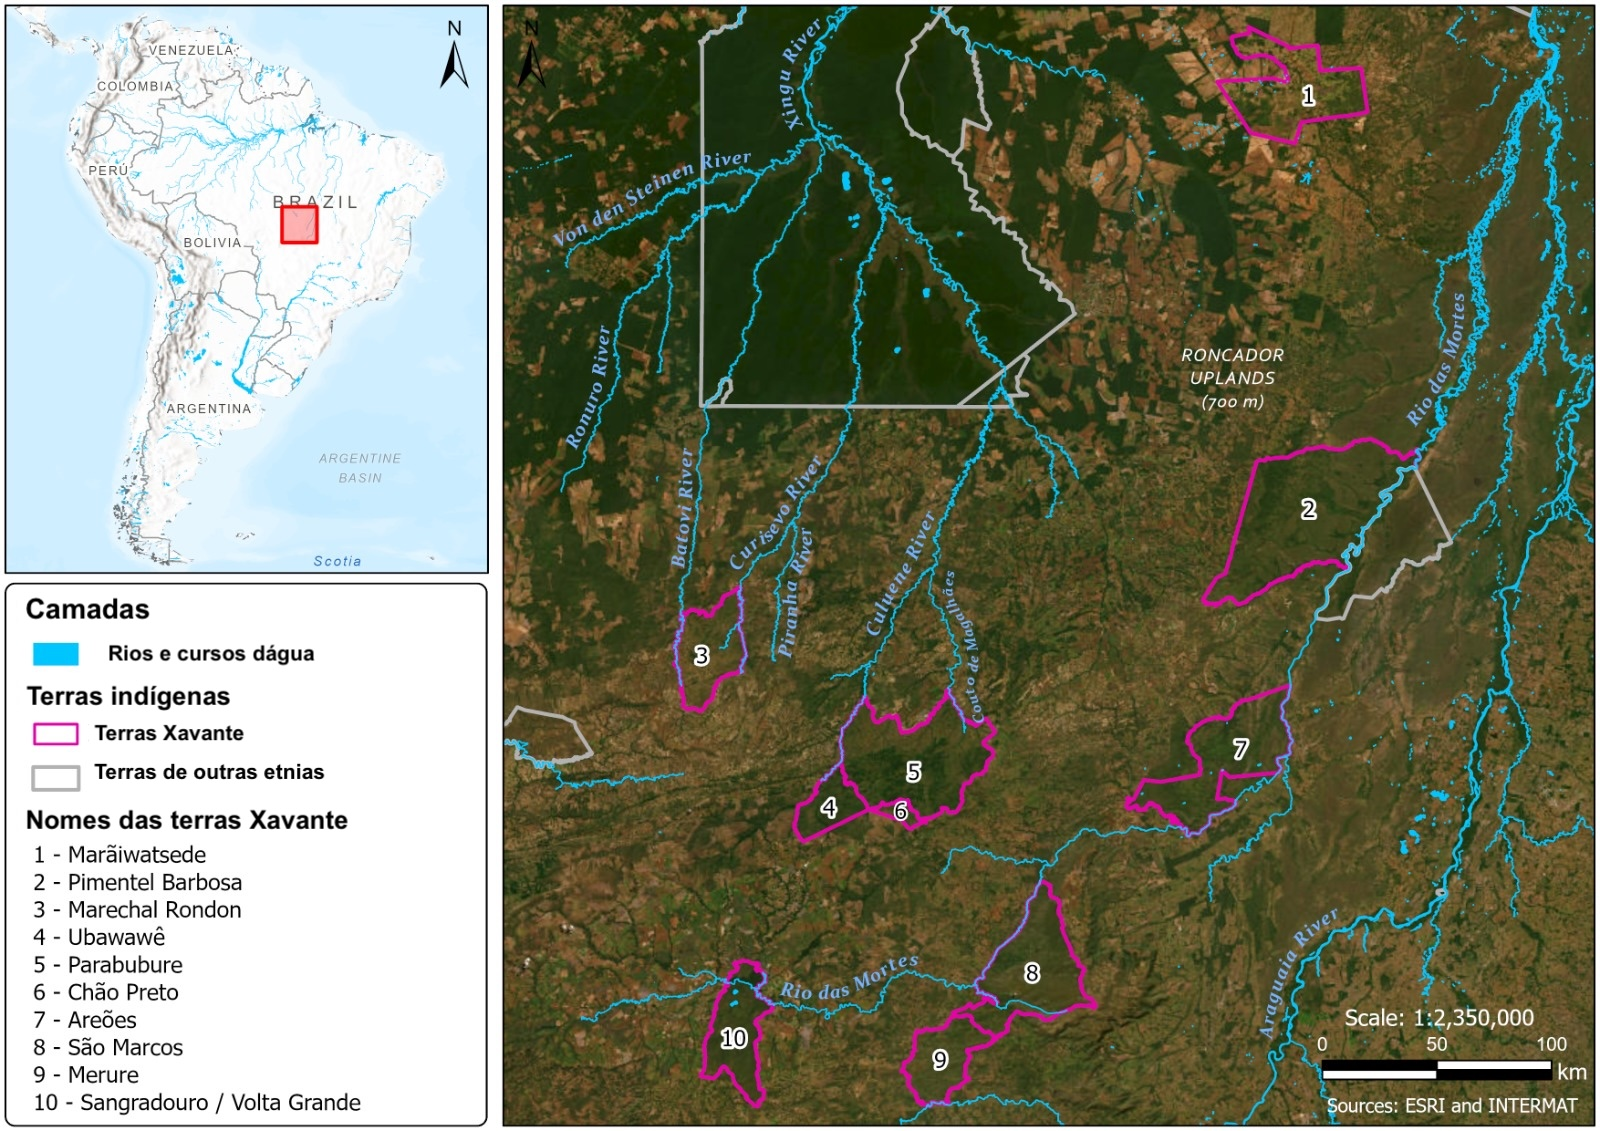
\includegraphics[width=0.7\linewidth]{XavanteTerras.jpeg}
    \caption{Terras indígenas Xavante}
    \label{fig:XavTerras}
\end{figure}

\section*{A língua Xavante}

A língua Xavante é uma das línguas indígenas mais faladas no Brasil. Com base em informações dos serviços de saúde e em nossas visitas a diversas aldeias localizadas em diferentes terras indígenas Xavante (ver Figura~\ref{fig:XavTerras}), estimamos que a população Xavante seja de aproximadamente 27 mil pessoas.

O Xavante pertence à família linguística Jê (Ferraz Gerardi et al. 2025), a qual, por sua vez, integra uma macrofamília proposta, a Macro-Jê — cuja composição ainda não é consensual na literatura (Nikulin 2020). Os Xavante (aʔuwẽ) e os Xerente (akuwẽ) formavam, até cerca de 210 anos atrás, um único povo. A cisão ocorreu a partir de sucessivas migrações do grupo que, segundo a tradição oral, “atravessou o rio” — este veio a constituir o povo Xavante.

Tipologicamente, o Xavante é uma língua quase isolante, porém com uma morfossintaxe relativamente complexa e um tipo raro de alinhamento morfossintático, observado apenas em algumas línguas da família Carib e em certos membros da família Jê.

O Xavante é falado como primeira língua em todas as aldeias, e muitos falantes não dominam o português, seja na sua modalidade oral ou escrita.

Nos últimos anos, observa-se um fenômeno de migração — ainda incipiente — de Xavantes para centros urbanos. Apesar de discreto, esse êxodo tem crescido, o que aponta para a urgência de políticas linguísticas capazes de antecipar desafios no planejamento linguístico da língua Xavante. É com essa preocupação que realizamos nosso trabalho de campo, cujo objetivo é, entre outros, documentar e descrever a língua Xavante, que, em nossa avaliação, ainda carece de uma descrição abrangente,  sistemática, e tipologicamente .


%########################################################################
\chapter*{Como usar o dicionário}

Este dicionário apresenta uma seleção de palavras da língua Xavante com suas respectivas traduções e informações gramaticais em português. Cada entrada foi formatada para facilitar o acesso e a compreensão por parte de falantes, professores, estudantes e pesquisadores.

\section*{Formato das entradas}

As entradas seguem o seguinte modelo:

\begin{quote}
\textbf{wéré} \textit{s.} -- pássaro preto, anu preto
\end{quote}

\begin{itemize}
  \item \textbf{Forma em negrito}: representa a palavra em Xavante.
  \item \textit{Abreviação em itálico}: indica a classe gramatical (por exemplo, \textit{s.} para substantivo, \textit{v.} para verbo).
  \item Após os dois traços (\texttt{--}), encontra-se a tradução ou explicação da palavra em português.
  \item Quando pertinente, formas variantes ou flexionadas são indicadas com exemplos adicionais em negrito.
\end{itemize}

\section*{Prefixo humano \textit{da-}}

Na língua Xavante, o prefixo \textit{da-} indica a categoria semântica de “ser humano” e pode aparecer como parte de muitos substantivos. Neste dicionário, entretanto, optou-se por registrar as palavras sem esse prefixo.

\begin{quote}
\textbf{da’wéra} “pessoa velha” aparece no dicionário como \textbf{’wéra}
\end{quote}

Portanto, ao procurar uma palavra que contenha o prefixo \textit{da-}, recomenda-se buscar a forma sem ele, pois o dicionário organiza as entradas de acordo com a raiz.

\section*{Abreviações utilizadas}

A lista completa de abreviações pode ser consultada na seção \textit{Abreviações}, mas as mais frequentes incluem:

\begin{description}[leftmargin=3cm, style=multiline]
  \item[s.] Substantivo
  \item[v.] Verbo
  \item[adv.] Advérbio
  \item[adj.] Adjetivo
  \item[intj.] Interjeição
  \item[vc.] Verbo com complemento
\end{description}

\section*{Observações adicionais}

\begin{itemize}
  \item Algumas traduções apresentam mais de um termo em português para abranger diferentes usos ou significados da palavra Xavante.
  \item As formas com prefixos como \textbf{ĩ-} indicam flexões pessoais e são incluídas como exemplos quando relevantes.
  \item Entradas compostas ou com significados culturais importantes podem incluir observações adicionais em edições futuras.
\end{itemize}

Esperamos que este dicionário seja útil para a aprendizagem, o ensino e a valorização da língua Xavante.

\chapter*{Abreviações}

\begin{description}[leftmargin=3cm, style=multiline]
  \item[S.] Substantivo
  \item[V.] Verbo
  \item[ADJ.] Adjetivo
  \item[INTJ.] Interjeição
  \item[ADV.] Advérbio
  \item[PRON.] Pronome
  \item[DET.] Determinante
  \item[DU.] Dual
  \item[PL.] Plural
  \item[POSP.] Posposição
  \item[S.] Singular
  \item[]
  \item[]
  
\end{description}

\frontmatter
\renewcommand{\contentsname}{Dicionário Xavante-Português} % Or your preferred title
\tableofcontents

\mainmatter

\chapter*{Dicionário Xavante-Português}

\textbf{a'a} [aʔa] \textit{S.} -- tosse.

\textbf{a'a wai'o} [aʔa waiʔo] \textit{S.} -- catarro, pigarro.

\textbf{a'a'a bö} [aʔaʔa bö] \textit{S.} -- penas de rabo de mutum.

\textbf{a'a'a pré} [aʔaʔa pré] \textit{S.} -- mutum vermelho.

\textbf{a'ama} [ʔaʔama] \textit{S.} -- advogado, defensor.

\textbf{a'amo na mrozé} [aʔamo na mrozé] \textit{S.} -- calendário, elenco dos meseS.}

\textbf{a'amo za'ru} [aʔamo zaʔru] \textit{S.} -- halo da lua.

\textbf{a'amo} [aʔamõ] \textit{S.} -- lua. -- [audio: audio/moon.wav]{\faHeadphones}. -- [image: https://upload.wikimedia.org/wikipedia/commons/thumb/e/e1/FullMoon2010.jpg/960px-FullMoon2010.jpg]

\textbf{a'eta} [aʔeta] \textit{S.} -- primavera.

\textbf{a'ẽta'a wi} [aʔẽtaʔa wi] \textit{S.} -- início de primavera.

\textbf{a'ẽta'a} [aʔẽtaʔa] \textit{S.} -- a'ẽta primavera.

\textbf{a'odo} [ʔaʔo'do] \textit{S.} -- côco, côco de bocaiúva.

\textbf{a'raté} [ʔaʔɾa'tɛ] \textit{S.} -- mãe de primeiro filho.

\textbf{a'rezé} [ʔaʔɾe'zɛ] \textit{S.} -- lumbago.

\textbf{a're} [ʔaʔ'ɾe] \textit{S.} -- anca, lombo.

\textbf{a're} [ʔaʔ'ɾe] \textit{S.} -- semente, planta pequena.

\textbf{a'a' riri} [aʔaʔ riri] \textit{S.} -- bronquite.

\textbf{a're} [aʔre] \textit{V.} -- plantar, semear.

\textbf{a'rã'ru bö} [aʔrãʔru bö] \textit{S.} -- rabo de mutum preto.

\textbf{a'rã'ru} [aʔrãʔru] \textit{S.} -- mutum.

\textbf{a'rã} [ʔaʔ'ɾã] \textit{V.}S.} -- assustar-se, admirar-se, comover-se, vencer, dominar.

\textbf{a'rãmi} [ʔaʔɾa'mĩ] \textit{V.}DU. assustar-se, admirar-se, comover-se, vencer, dominar.

\textbf{a'ré} [ʔaʔɾɛ] \textit{ADV.} -- quase, já.

\textbf{a'u'ö} [ʔaʔu'ʔə] \textit{V.} -- secar, enxugar

\textbf{dasi'u'ö} [dasiʔu'ʔə] \textit{V.}RFX. enxugar-se.

\textbf{a'ubuni} [ʔaʔubu'nĩ] \textit{S.} -- arbusto, matagal, mato denso, privada.

\textbf{a'urĩrĩ} [ʔaʔuɾĩ'ɾĩ] \textit{V.} -- limpar, encerar, acercar, dar volta.

\textbf{a'uréiwi} [aʔuréiwi] \textit{ADV.} -- nu, exposto, descoberto.

\textbf{itsito} [itsito] \textit{ADJ.} -- coberto, fechado.

\textbf{ai'utepré} [ʔaʔutepɾɛ] \textit{S.} -- bebê, criança recém-nascida.

\textbf{a'uwẽ nhib'ri} [ʔaʔuwẽɲĩbʔɾi] \textit{S.} -- casa do índio, cabana.} [image: https://www.aldeiamultietnica.com.br/img/casas/casa-xavante-sq.jpg]

\textbf{a'uwẽ nhibro} [ʔaʔuwẽɲĩbʔɾo] \textit{S.} -- lugar do índio, colônia indígena, terra de índioS.}

\textbf{a'uwẽ nhimirob'ru} [aʔuwẽ nhimirobʔru] \textit{S.} -- democracia.

\textbf{a'uwẽ pisudu} [aʔuwẽ pisudu] \textit{S.} -- cabeça.

\textbf{a'uwẽ siwazari} [aʔuwẽ siwazari] \textit{S.} -- mestiço.

\textbf{a'uwẽ ubumro} [aʔuwẽ ubumro] \textit{S.} -- reunião dos homens, comunidade, povo.

\textbf{a'uwẽ wa're zapu} [aʔuwẽ waʔre zapu] \textit{S.} -- furo da orelha.

\textbf{a'uwẽ zéré} [aʔuwẽ zéré] \textit{S.} -- cabelo de índio.

\textbf{a'uwẽ} [ʔaʔuwẽ] \textit{S.} -- pessoa, gente, xavante.

\textbf{a'ãma sipi'ö} [aʔãma sipiʔö] \textit{S.} -- advogada, defensora.

\textbf{a'é} [ʔa'ʔɛ] \textit{S.} -- semente de capim navalha, colar de semente de capim navalha, pedra.

\textbf{a'öiwãtizu} [ʔaʔəiwãti'zu] \textit{S.} -- incenso, resina.

\textbf{a'öpé} [ʔaʔə'pɛ] \textit{INTJ. atenção! espere!

\textbf{a'öza} [ʔaʔəza] \textit{INTJ. espera! deixa assim!.

\textbf{a'ö} [ʔa'ʔə] \textit{INTJ. espera! ainda, por enquanto.

\textbf{a'õ} [ʔa'ʔə] \textit{S.} -- jatobá. ([link: https://pt.wikipedia.org/wiki/Jatobá]Hymenaea courbaril)} [image: https://upload.wikimedia.org/wikipedia/commons/thumb/5/5c/Hymenaea_courbaril_1.jpg/960px-Hymenaea_courbaril_1.jpg]

\textbf{a'ö} [ʔa'ʔə] \textit{V.} -- tãma a'ö mono dar água.

\textbf{a'ö} [ʔa'ʔə] \textit{V.} -- pegar água.

\textbf{a-} [a-] \textit{ip. 2ª pessoa. ana 'tua mãe'.

\textbf{ab're} [ʔab'ʔɾe] \textit{S.} -- buraco, cova, cavidade.

\textbf{ab're} [ʔab'ʔɾe] \textit{V.} -- cavar, fazer buraco, enterrar.

\textbf{ab'ruti'i} [ʔabʔɾuti'ʔi] \textit{V.} -- enfurecer, zangar.

\textbf{ab'ru} [ʔab'ʔɾu] \textit{ADJ.} -- zangado, irado

\textbf{ab'rã} [ʔab'ʔɾã] \textit{S.} -- última casa da aldeia.

\textbf{ab'é'rã} [ʔabʔɛ'ʔɾã] \textit{S.} -- mussurana.

\textbf{aba'ẽ} [ʔaba'ʔẽ] \textit{V.} -- convencer da'ãma -- aba'ẽ convencer alguém.

\textbf{aba'wa} [ʔaba'ʔwa] \textit{S.} -- caçador.

\textbf{abada} [ʔaba'da] \textit{S.} -- esposa sem filhoS.}

\textbf{abahi 'rãi pré} [abahi ʔrãi pré] \textit{S.} -- fruta vermelha do mato.

\textbf{abahi 'ãiprére} [abahi ʔãiprére] \textit{S.} -- cereja.} [image: https://upload.wikimedia.org/wikipedia/commons/thumb/9/94/Black_Che.jpg/500px-Black_Che.jpg]

\textbf{abahi wede ro} [abahi wede ro] \textit{S.} -- pomar (lugar de árvore de fruta).

\textbf{abahi} [ʔaba'hi] \textit{S.} -- fruta (termo geral).

\textbf{abamere} [ʔabamẽɾe] \textit{S.} -- cestinho redondo.

\textbf{abame} [ʔabamẽ] \textit{S.} -- cesto redondo.

\textbf{abanhinheme ubumro} [abanhinheme ubumro] \textit{S.} -- bagagem.

\textbf{abanhinhemere} [abanhinhemere] \textit{S.} -- cestinho com tampa.

\textbf{abare'u} [ʔabaɾe'ʔu] \textit{S.} -- piqui.

\textbf{abare'u} [ʔabaɾe'ʔu] \textit{S.} -- nome de grupo etário.

\textbf{abanhizé} [ʔabaɲĩ'zɛ] \textit{S.} -- baquité (cesto) com tampa, mala.

\textbf{abare} [ʔaba'ɾe] \textit{S.} -- bucho de animal ruminante.

\textbf{abare} [ʔaba'ɾe] \textit{S.} -- piqui.

\textbf{abarudu} [ʔabaɾu'du] \textit{S.} -- árvore de embira (gênero} [link: https://pt.wikipedia.org/wiki/Daphnopsis]Daphnopsis)} [image: https://upload.wikimedia.org/wikipedia/commons/8/86/Daphnopsis_hellerana.jpg]abawazi} [ʔabawa'zi] \textit{S.} -- timbó.

\textbf{abaze zahi} [abaze zahi] \textit{S.} -- animal ferroz, fera.

\textbf{abazei hö} [aba'zei'hə] \textit{S.} -- couro, pele de animal.

\textbf{abaze} [aba'ze] \textit{S.} -- caça, animal de caça.} [audio: audio/animal.wav]

\textbf{abazi dumnarĩ} [abazi dumnarĩ] \textit{S.} -- algodão sem caroço.

\textbf{abazi zanhamri} [abazi zanhamri] \textit{S.} -- tecido tecido de algodão.

\textbf{abazinheme} [abazinheme] \textit{S.} -- = abazizé -- cesto con tampa, baquité com tampa. abaziparazu} [abazinheme] \textit{S.} -- rede.

\textbf{abazipara} [ʔabazipaɾa] \textit{S.} -- rede.

\textbf{abazizé = abanhizé} [abazizé = abanhizé] \textit{S.} -- cesto com tampa, baquité com tampa.

\textbf{abazi} [ʔabazi] \textit{S.} -- algodão, fio de algodão, linha.

\textbf{aba} [ʔaba] \textit{S.} -- caça.

\textbf{abzaihö} [ʔabzai'hə] \textit{V.} -- espirrar terra.

\textbf{abzuma} [ʔabzu'mã] \textit{ADV.} -- ao meio dia, de meio dia.

\textbf{abzuma} [ʔabzu'mã] \textit{S.} -- meio dia.

\textbf{abzé} [ʔab'zɛ] \textit{S.} -- veneno de feitiço, pó de casca para feitiço, doença.

\textbf{abzö} [ʔab'zə] \textit{S.} -- tipo de marimbondo.

\textbf{ĩwasede} [ĩwasede] \textit{ADJ.} -- feio, selvagem.} [audio: audio/ugly.wav]

\textbf{adabasa} [ʔabada'sa] \textit{S.} -- comida de jovem casada, casamento.

\textbf{adumhöprã} [adumhöprã] \textit{S.} -- mulher recém-grávida.

\textbf{adu} [ʔa'du] \textit{S.} -- barriga, estômago, abdômen.

\textbf{adö'ö 'rai hi} [adöʔö ʔrai hi] \textit{S.} -- caveira, crânio (osso da cabeça do defunto).

\textbf{adö'ö'ru} [adöʔöʔru] \textit{S.} -- cemitério, sepultura.

\textbf{adö'ö'ru} [ʔadəʔə'ʔɾu] \textit{S.} -- lugar dos falecidoS.}

\textbf{adö} [ʔa'də] \textit{S.} -- defunto, falecido, cadáver, morte.

\textbf{ahu na} [ahu na] \textit{?. pegue água.

\textbf{ahu'rã} [ʔahu'ʔɾã] \textit{S.} -- pintura de carvão.

\textbf{ahupré} [ʔahu'pɾɛ] \textit{S.} -- encerramento do ritual.

\textbf{ahömhö amoi wa} [ahömhö amoi wa] \textit{ADV.} -- ante ontem.

\textbf{ahömhö} [ahömhö] \textit{ADV.} -- ontem.

\textbf{ahö} [ʔahə] \textit{ADJ.} -- ĩ'ahö bastante, muito, maiS.}

\textbf{ahö} [ʔahə] \textit{V.} -- aumentar, aumentar gente, acrescentar.

\textbf{ahöri} [ʔahəɾi] \textit{V.} -- bater, surrar, castigar batendo.

\textbf{ai'a're} [aiʔaʔre] \textit{S.} -- lado do tórax de uma pessoa.

\textbf{ai'aba'ré} [aiʔabaʔré] \textit{V.}PL. ir, andar, caminhar.

\textbf{ai'are} [aiʔare] \textit{S.} -- dente.

\textbf{ai'ratare} [ʔaiʔɾataɾɛ] \textit{S.} -- velho, idoso.

\textbf{ai'raté} [ʔaiʔɾatɛ] \textit{S.} -- mulher de um filho.

\textbf{ai'rere} [ʔaiʔɾe'ɾe] \textit{S.} -- arbusto de côco, grupo etário.

\textbf{ai'ro} [ʔai'ʔɾo] \textit{S.} -- fezeS.}

\textbf{ai'ré} [ʔai'ʔɾɛ] \textit{V.} -- ir, afastar-se, separar, progredir, crescer, avançar.

\textbf{ai'ubuni} [ʔaiʔubu'nĩ] \textit{V.} -- contestar, retrucar, mentir.

\textbf{ai'udö} [ʔaiʔu'də] \textit{V.} -- enganar, mentir.

\textbf{ai'uirĩ} [ʔaiʔui'ɾĩ] \textit{V.} -- rodar.

\textbf{ai'uiréiwa} [aiʔuiréiwa] \textit{ADV.} -- abertamente, claramente.

\textbf{ai'uréwi} [ʔaiʔuɾɛwi] \textit{ADJ.} -- claro, aberto.

\textbf{ai'uté mreme tétére} [aiʔuté mreme tétére] \textit{S.} -- balbuciar.

\textbf{ai'uté nhanapré} [aiʔuté nhanapré] \textit{S.} -- verme de criança.

\textbf{ai'uté podo} [aiʔuté podo] \textit{S.} -- convívio matrimonial, coito, relacionamento sexual.

\textbf{ai'uté potore} [aiʔuté potore] \textit{S.} -- boneca.

\textbf{ai'uté wa} [aiʔuté wa] \textit{S.} -- vencedor, campeão =

\textbf{ai'uté} [ʔaiʔu'tɛ] \textit{S.} -- criança.

\textbf{ai'uté} [aiʔuté] \textit{V.} -- alcançar, conseguir, vencer. -- wa ãma ai'uté. nós o alcançamos, nós o conseguimos, nós o vencemoS.}

\textbf{ai'utörĩ} [aiʔutörĩ] \textit{V.} -- terminar, acabar, definhar, morrer.

\textbf{ai'utö} [ʔaiʔu'tə] \textit{V.}SG. terminar, definhar, morrer, acabar.

\textbf{ai'wapé} [ʔaiʔwa'pɛ] \textit{V.}DU. combater, lutar, guerrear, concorrer.

\textbf{a(i)-} [ai] \textit{IP. índice preso de 2ª pessoa.

\textbf{aiba} [aiba] \textit{V.} -- compadecer-se, ter amor, ter pena, ter paciência.

\textbf{aibö nhimihöze} [aibö nhimihöze] \textit{S.} -- homem que gosta de briga, homem briguento.

\textbf{aibö toire} [aibö toire] \textit{S.} -- palhaço, homem que gosta de brincadeira.

\textbf{aibötoire} [aibötoire] \textit{S.} -- palhaço, brincalhão.

\textbf{aibö} [ʔai'bə] \textit{S.} -- homem, macho.} [audio: audio/man.wav]

\textbf{aihini} [ʔaihi'nĩ] \textit{PRON. todoS.}

\textbf{aihutu} [ʔaihu'tu] \textit{V.}PL. chegar, alcançar.

\textbf{aihu} [ʔai'hu] \textit{S.} -- brinco.

\textbf{aihö hö} [ʔai'hə'hə] \textit{S.} -- couro de veado.

\textbf{aihö nhimi'wa} [aihö nhimiʔwa] \textit{S.} -- unha de veado.

\textbf{aihö'ubuni} [aihöʔubuni] \textit{S.} -- wapté de orelha furada, wapté que é chefe do grupo.

\textbf{aihöi'ré} [ʔaihəiʔɾɛ] \textit{S.} -- jacaré.} [image: https://upload.wikimedia.org/wikipedia/commons/thumb/d/df/Caiman_crocodilus_llanoS.}JPG/500px-Caiman_crocodilus_llanoS.}JPG]} [audio: ]

\textbf{aihö} [ʔaihə] \textit{S.} -- veado-campeiro ([https://pt.wikipedia.org/wiki/Veado-campeiro]Blastocerus campestris).} [image: https://upload.wikimedia.org/wikipedia/commons/thumb/b/b8/O._bezoarticus_buck.jpg/960px-O._bezoarticus_buck.jpg]

\textbf{aihö} [ʔaihə] \textit{V.} -- rir, sorrir.

\textbf{aima'uri} [ʔaimãʔuɾi] \textit{V.} -- esconder, esconder-se.

\textbf{aima'wara} [ʔaimãʔwaɾa] \textit{V.}DU. fazer subir, empoleirar, ficar de pé.

\textbf{aima'wa} [aimaʔwa] \textit{V.}SG./du. = aima'wara = dasima'wara -- fazer subir, empoleirar, ficar de pé. aimani} [aimaʔwa] \textit{V.} -- fugir, perder-se.

\textbf{aimasa} [aimasa] \textit{V.}PL.} [aimasa] \textit{dasimasa = dasima'wara} [aimasa] \textit{V.}DU. ficar de pé, encontrar-se.

\textbf{aimasisi} [ʔaimãsisi] \textit{V.}DU. estar, ficar, chegar, ser, estar, comparecer, apresentar-se.

\textbf{aimawi a'uwẽ} [ʔaimawiʔaʔuwẽ] \textit{ADJ.} -- índio não xavante.

\textbf{aimawi} [ʔaimawi] \textit{ADJ.} -- diferente, outro.

\textbf{aimawi} [aimawi] \textit{S.} -- cláusula.

\textbf{aime} [aimẽ] \textit{V.}SG.} [dasimẽ] \textit{dasime = dasiwabzuri} [dasiwabzuɾi] \textit{V.}DU. deitar-se, jogar-se, meter-se

\textbf{da'ãma dasiwãri} [daʔãma dasiwãri] \textit{V.} -- ajudar aime na ajude-me! aiparapisudu} [daʔãma dasiwãri] \textit{S.} -- cavalo.

\textbf{aipi'ra} [aipiʔra] \textit{V.}SG.} [aipiʔra] \textit{dasipi'ra = dasipizari} [aipiʔra] \textit{V.}DU./pl. virar-se, voltar-se.

\textbf{aipo'o} [aipoʔo] \textit{V.} -- = po'o -- quebrar, partir, rachar, romper-se. aipuru} [aipoʔo] \textit{V.} -- ĩpru quebrar-se, romper.

\textbf{aipé} [ʔaipɛ] \textit{V.} -- dividir, cortar em pedaços, espalhar, dissipar.

\textbf{aire} [aire] \textit{V.} -- aire na -- dê! entregue!

\textbf{airãzapotore} [aire] \textit{S.} -- ?.

\textbf{aiwa ĩnomri} [aiwa ĩnomri] \textit{S.} -- compensação.

\textbf{aiwa'aba -- no meio de dois S.} -- aiwa'aba} [aiwaʔaba]

\textbf{?} [?] \textit{V.} -- condenar, executar.

\textbf{aiwa'ro} [ʔaiwaʔɾo] \textit{S.} -- sol.

\textbf{aiwa'u} [ʔaiwa'ʔu] \textit{S.} -- água.

\textbf{aiwa'õ} [ʔaiwaʔõ] \textit{S.} -- choro.

\textbf{aiwa'öno} [aiwaʔöno] \textit{S.} -- separação.

\textbf{aiwa'õ} [aiwaʔõ] \textit{V.} -- chorar.

\textbf{aiwa'ötöre} [aiwaʔötöre] \textit{S.} -- olho.

\textbf{aiwa'ö} [aiwa'ʔə] \textit{LEX. choro, chorar.

\textbf{aiwahi'ãsi} [aiwahiʔãsi] \textit{S.} -- cerimônia para curar doença.

\textbf{aiwahudu} [aiwahudu] \textit{V.} -- levantar-se, erguer-se.

\textbf{aiwamri} [aiwamri] \textit{V.} --  dawamri sossegar, acalmar-se, ter calma. aiwanarĩwarĩrĩzé} [aiwamri] \textit{S.} -- sal.

\textbf{aiwanarĩzeire} [aiwanarĩzeire] \textit{S.} -- biscoito, bolacha.

\textbf{aiwanhizari} [aiwanhizari] \textit{V.} -- separar, afastar, apartar.

\textbf{aiwanhiza} [aiwanhiza] \textit{V.}SG.  aiwanhi zari -- separar, afastar, apartar. aiwapsari} [aiwanhiza] \textit{V.} -- resmungar, murmurar, criticar, queixar-se.

\textbf{aiwapsisi} [aiwapsisi] \textit{V.}DU.PL. dançar.

\textbf{aiwapsi = aiwa} [aiwapsi = aiwa] \textit{ADV.} -- igualmente, semelhante, assim.

\textbf{aiwazure} [aiwazure] \textit{S.} -- cabelo.

\textbf{aiwa} [aiwa] \textit{ADV.} -- igual, semelhante, assim.

\textbf{aiwapsi} [aiwapsi] \textit{ADV.} -- igual, semelhante, assim.

\textbf{aiwẽ'ẽ} [aiwẽʔẽ] \textit{V.} -- inclinar-se, sair às pressas, disparar em corrida.

\textbf{ai'are} [aiʔa'ɾe] \textit{S.} -- dente.

\textbf{a ĩ'ai mo} [a ĩʔai mo] \textit{S.} -- dar comida, alimentar.

\textbf{ai'rowi} [aiʔɾowi] \textit{S.} -- capivara.

\textbf{ai'rãjhõrõ} [aiʔrãjhõrõ] \textit{S.} -- urubu.

\textbf{ai'rãzapotore} [aiʔrãzapotore] \textit{S.} -- macaco.

\textbf{ai'uza} [ai'ʔuza] \textit{S.} -- homem branco.

\textbf{ai'wapesere} [aiʔwapesere] \textit{S: rato.

\textbf{ai'waza'é} [aiʔwaza'ʔɛ] \textit{S.} -- cachorro.

\textbf{ai'wanhirã} [aiʔwañirã] \textit{S.} -- tamanduá-bandeira. ([link: https://pt.wikipedia.org/wiki/Tamanduá-bandeira]Myrmecophaga tridactyla)} [image: https://upload.wikimedia.org/wikipedia/commons/thumb/3/3b/Myresluger2.jpg/560px-Myresluger2.jpg]} [audio: ]

\textbf{ai'ãpu} [aiʔãpu] \textit{V.} -- falar.

\textbf{ai'ãpu} [aiʔãpu] \textit{V.} -- falar.

\textbf{aiböihöbö} [aiböihöbö] \textit{S.} -- quati. ([link: ])} [image: ]} [audio: ]

\textbf{aiparapisudu} [aiparapisudu] \textit{S cavalo. ([link: ])} [image: ]} [audio: ]

\textbf{aiparapo} [aiparapo] \textit{S.} -- pato. ([link: ])} [image: ]} [audio: ]

\textbf{aipesere} [aipesere] \textit{S.} -- queixada. ([link: ])} [image: ]} [audio: ]

\textbf{aipe} [aipe] \textit{S.} -- porco-do-mato. ([link: ])} [image: ]} [audio: ]

\textbf{aipi} [aipi] \textit{S.} -- chuva.

\textbf{aiwa'õtõre} [aiwaʔõtõre] \textit{S.} -- olho.

\textbf{ame!} [ame!] \textit{excl. infa}. mãe! amere} [ame!] \textit{excl. infa. maezinha!

\textbf{amhuri} [amhuri] \textit{S.} -- lepra.

\textbf{amhözépa sina marĩ 'ru} [amhözépa sina marĩ ʔru] \textit{S.} -- chantagem. amhözépa} [amhözépa sina marĩ ʔru] \textit{S.} -- ameaça, tribulação.

\textbf{amiro} [amiro] \textit{S.} -- centopéia.

\textbf{amiruru'wa} [amiruruʔwa] \textit{S.} -- lagarta de fogo.

\textbf{amnhana} [amnhana] \textit{V.}PL} [amnhana] \textit{danhimnhana = daza'o} [amnhana] \textit{V.}DU. pender, pendurar.

\textbf{amnhasi} [amnhasi] \textit{V.} -- pedir a quem tem, desconfiar.

\textbf{amnhatã} [amnhatã] \textit{V.}PL. c.} [amnhatã] \textit{danhimnhana = daza'o} [amnhatã] \textit{V.}DU. pender, pendurar.

\textbf{amnho za'warizé} [amnho zaʔwarizé] \textit{S.} -- armazém.

\textbf{amnho'a} [amnhoʔa] \textit{S.} -- trigo.

\textbf{amnho'rã} [amnhoʔrã] \textit{S.} -- centeio.

\textbf{amnho'rézé} [amnhoʔrézé] \textit{S.} -- secador de cereaiS.}

\textbf{amnho'ubumrozé} [amnhoʔubumrozé] \textit{S.} -- lugar de reunir os cereais, silo, celeiro.

\textbf{amnhonhimnhorö} [amnhonhimnhorö] \textit{S.} -- cevada.

\textbf{amnhotehöri} [amnhotehöri] \textit{V.} -- ceifar, colher.

\textbf{amnhotepezé} [amnhotepezé] \textit{S.} -- março.

\textbf{amnho} [amnho] \textit{S.} -- cereal.

\textbf{amo'wa} [amoʔwa] \textit{S.} -- outro, companheiro falecido.

\textbf{amo} [amo] \textit{ADJ.} -- ĩ'amo outro.

\textbf{amo} [amo] \textit{S.} -- companheiro, colega, camarada.

\textbf{anarowa} [anarowa] \textit{S.} -- grupo etário.

\textbf{ana} [ana] \textit{prep. pessoa/ S.} -- tua mãe, sua mãe (de você).

\textbf{ana} [ana] \textit{V.}} [ana] \textit{da'ãma ana = da'ãma dasina -- ajudar, servir. ane} [ana] \textit{S.} -- veado, cervo.

\textbf{anhana'rãtömri} [anhanaʔrãtömri] \textit{S.} -- lagarta preta.

\textbf{anhana'upi} [anhanaʔupi] \textit{S.} -- besouro.

\textbf{anhana} [anhana] \textit{S.} -- esterco, estrume.

\textbf{anhidazari} [anhidazari] \textit{V.} -- matar, acabar com.

\textbf{anhisisi} [anhisisi] \textit{V.} -- afastar, livrar.

\textbf{anhiza} [anhiza] \textit{V.} -- chegar ao grupo, alcançar alguém.

\textbf{anhomri} [anhomri] \textit{V.} -- sömri engolir, dar muito.

\textbf{anhoré = danhoré} [anhoré = danhoré] \textit{V.} -- enfileirar

\textbf{romnhoré} [romnhoré] \textit{V.} -- estudar. anhĩsu = sisu -- colocar penas em flecha. anomri} [romnhoré] \textit{V.} -- ir.

\textbf{apa} [apa] \textit{S.} -- lagartixa.

\textbf{apapa} [apapa] \textit{S.} -- ([link: https://pt.wikipedia.org/wiki/Scolopendridae]lacraia).} [image: https://upload.wikimedia.org/wikipedia/commons/thumb/1/15/Scolopendra_polymorpha_1.jpg/560px-Scolopendra_polymorpha_1.jpg]

\textbf{apapa wanhiodo} [IPA] \textit{S.} -- ([link: https://pt.wikipedia.org/wiki/Escorpião]escorpião)} [image: https://upload.wikimedia.org/wikipedia/commons/thumb/8/8d/Asian_forest_scorpion_in_Khao_Yai_National_Park.JPG/960px-Asian_forest_scorpion_in_Khao_Yai_National_Park.JPG]

\textbf{api'ra} [apiʔra] \textit{V.}SG. = dasipiza} [apiʔra] \textit{V.}DU. tombar, virar-se.

\textbf{api} [api] \textit{V.} -- cozinhar.

\textbf{apsaihuri} [apsaihuri] \textit{V.} -- roubar.

\textbf{apsi nhoro} [apsi nhoro] \textit{S.} -- fibra de broto de gravatá.

\textbf{apsi} [apsi] \textit{S.} -- gravatá, abacaxi.

\textbf{apto'oré} [aptoʔoré] \textit{ADV.} -- mais tarde.

\textbf{aptorore} [aptorore] \textit{S.} -- nhambu.

\textbf{aptoro} [aptoro] \textit{V.} -- fazer flechas para caça.

\textbf{aptö'özé} [aptöʔözé] \textit{S.} -- cansaço, sono.

\textbf{aptö'ö} [aptöʔö] \textit{ADJ.} -- cansado, com sono, exausto.

\textbf{aptömri'a} [aptömriʔa] \textit{S.} -- cera branca.

\textbf{aptömriro'o zabzé} [aptömriroʔo zabzé] \textit{S.} -- lugar de pör a luz de cera, castiçal.

\textbf{aptömriro} [aptömriro] \textit{S.} -- luz de cera, vela.

\textbf{aptömri} [aptömri] \textit{S.} -- cera preta.

\textbf{aptö} [aptö] \textit{S.} -- sono, cansaço.

\textbf{apö sihöiba} [apö sihöiba] \textit{adV.}/ V.} -- apö dasihöiba ressuscitar, voltar à vida.

\textbf{apöre} [apöre] \textit{ADV.} -- outra vez.

\textbf{apösi} [apösi] \textit{ADV.} -- depois, mais tarde, só na volta.

\textbf{apö} [apö] \textit{ADV.} -- outra vez, de volta, depoiS.}

\textbf{ari'iwi} [ariʔiwi] \textit{ADV.} -- quieto, silencioso.

\textbf{arãrã nhi'u} [arãrã nhiʔu] \textit{S.} -- suco que o beija-flor tira, néctar, suco de flor.

\textbf{arãrã'rã} [arãrãʔrã] \textit{S.} -- beija-flor preto.

\textbf{arãrãre} [arãrãre] \textit{S.} -- colibri.

\textbf{arãrã} [arãrã] \textit{S.} -- beija-flor.

\textbf{asa'ẽtẽ nhi} [asaʔẽtẽ nhi] \textit{S.} -- carne de anta.

\textbf{asabutéi'wa} [asabutéiʔwa] \textit{S.} -- moço iniciado.

\textbf{asabu} [asabu] \textit{S.} -- casa.

\textbf{asada'a tei hi} [asadaʔa tei hi] \textit{S.} -- osso de canela de onça parda.

\textbf{asada'a} [asadaʔa] \textit{S.} -- asada puma, onça parda.

\textbf{asada'rã} [asadaʔrã] \textit{S.} -- lobo guará.

\textbf{asada} [asada] \textit{S.} -- puma, onça parda.

\textbf{asadö} [asadö] \textit{S.} -- camaleão, tiú.

\textbf{asahöpöre} [asahöpöre] \textit{S.} -- unha.

\textbf{asamrohöbö} [asamrohöbö] \textit{S.} -- ouriço chato.

\textbf{asamro} [asamro] \textit{S.} -- ouriço, ouriço cacheiro.

\textbf{asamro} [asamro] \textit{V.}DU. correr.

\textbf{asanaze} [asanaze] \textit{S.} -- preã.

\textbf{asarob'rãihörizé} [asarobʔrãihörizé] \textit{S.} -- coiS.}om que S.}orta a cacho do cereal, colheitadeira.

\textbf{asaro} [asaro] \textit{S.} -- arroz.

\textbf{asarébé'a} [asarébéʔa] \textit{S.} -- tipo de peixe.

\textbf{asaröno} [asaröno] \textit{V.} -- pular muito.

\textbf{asarötöpe} [asarötöpe] \textit{S.} -- bola.

\textbf{asimro} [asimro] \textit{V.}PL.} [asimro] \textit{da'ubumro = dasimasisi} [asimro] \textit{V.}DU. unir-se, ficar, sentar-se.

\textbf{asisi} [asisi] \textit{V.}PL.} [asisi] \textit{danhisisi = dazsi} [asisi] \textit{V.}DU. entrar, seguir.

\textbf{asã'ẽne} [asãʔẽne] \textit{S.} -- anta.

\textbf{asérére umo} [asérére umo] \textit{S.} -- pauzinho de buritirana.

\textbf{asérére} [asérére] \textit{S.} -- buritirana.

\textbf{ati} [ati] \textit{V.}} [ati] \textit{ĩti = dati -- escolher. ato} [ati] \textit{S.} -- corcunda.

\textbf{atébré} [atébré] \textit{V.} -- proliferar, ter filhoS.}

\textbf{atébré} [atébré] \textit{S.} -- orvalho.

\textbf{atéma} [atɛma] \textit{ADV.} -- devagar.} [audio: audio/slowly.wav]

\textbf{awa'öbö} [awaʔöbö] \textit{V.} -- pagar, recompensar.

\textbf{awaibu} [awaibu] \textit{V.}PL. = mrami} [awaibu] \textit{V.}DU. pegar muito.

\textbf{awaru 'mapraba'wa ubumro} [awaru ʔmaprabaʔwa ubumro] \textit{S.} -- cavalaria.

\textbf{awaru 'mapraba'wa} [awaru ʔmaprabaʔwa] \textit{S.} -- cavaleiro.

\textbf{awaru 'mapraba} [awaru ʔmapraba] \textit{V.} -- cavalgar, montar cavalo.

\textbf{awaru ba'ömore} [awaru baʔömore] \textit{S.} -- jumentinho.

\textbf{awaru butu zéré} [awaru butu zéré] \textit{S.} -- cabelo do pescoço do cavalo, crina.

\textbf{awaru po're pa} [awaru poʔre pa] \textit{S.} -- cavalo de orelha comprida.

\textbf{awarubati} [awarubati] \textit{S.} -- camelo.

\textbf{awarupo'repa} [awarupoʔrepa] \textit{S.} -- burro.

\textbf{awarupo'repore} [awarupoʔrepore] \textit{S.} -- jumentinho.

\textbf{awarupo'repo} [awarupoʔrepo] \textit{S.} -- jumento, burro.

\textbf{awaru} [awaru] \textit{S.} -- neo. cavalo.

\textbf{awatis} [awatis] \textit{V.} -- amarrar.

\textbf{awati} [awati] \textit{V.} -- prensar, endireitar, subjugar, vencer.

\textbf{awa} [awa] \textit{S.} -- nome de árvore.

\textbf{awa} [awa] \textit{S.} -- sombra, assombração.

\textbf{awẽ} [awẽ] \textit{ADV.} -- amanhã.

\textbf{awẽ} [awẽ] \textit{V.} -- amanhecer

\textbf{ma tö ti'awẽ amanheceu. awã'awi} [ma tö tiʔawẽ amanheceu. awãʔawi] \textit{ADV.} -- já, logo, agora.

\textbf{awãrã} [awãrã] \textit{S.} -- mato, nome de árvore, arbusto reto.

\textbf{awã} [awã] \textit{S.} -- arbusto que faz sombra.

\textbf{awẽmhã} [awẽmhã] \textit{adv {amanhã}

\textbf{aza'ra} [azaʔra] \textit{V.} -- ĩsa'ra amontoar, arrumar, deixar, ficar, colocar, botar, pôr, agir.

\textbf{aza'ré} [azaʔré] \textit{V.} -- ĩsa're dar prazo, dar tempo.

\textbf{aza'ré} [azaʔré] \textit{V.} -- entregar, trair, ceder, afaster.

\textbf{azahu pisudu} [azahu pisudu] \textit{S.} -- penacho de arara com pouca pena.

\textbf{azahu} [azahu] \textit{S.} -- penacho de arara e outroS.}

\textbf{azani} [azani] \textit{V.} -- ĩsani tirar, afastar, livrar, afugentar.

\textbf{azarudu} [azarudu] \textit{S.} -- moça.

\textbf{azarutu} [azarutu] \textit{S.} -- moça.

\textbf{aze} [aze] \textit{S.} -- açúcar.

\textbf{azidi} [azidi] \textit{V.} -- fiar.

\textbf{azo} [azo] \textit{S.} -- anzol (empréstimo do português).

\textbf{azöri V.} -- bater, surrar, castigar batendo.

\textbf{a1} [a] \textit{ADJ.} -- branco. -- wede a = madeira branca.

\textbf{a2} [a] \textit{PRON. marca de 2a pessoa.

\textbf{a3} [a] \textit{S.} -- tosse.

\textbf{a4} [a] \textit{V.} -- da'a tossir, pingar, cair pingando ö ha, te ti'a'a ele tosse, ele pinga.

\textbf{a5} [a] \textit{V.} -- dar ö hã, ma tãma ti'a ele lhe deu ima a na dê-me, ajude-me.

\textbf{ãhã na} [ãhã na] \textit{ADV.} -- por aqui, seguindo por aqui.

\textbf{ãhã ta, wa ĩhöiba -- eu estou aqui, eu estou presente, presente! ãhã ta -- aqui!está aqui! ãhãna} [ãhã ta, wa ĩhöiba -- eu estou aqui, eu estou presente, presente! ãhã ta -- aqui!está aqui! ãhãna] \textit{ADV.} -- hoje, agora.

\textbf{awa'awi} [awaʔawi] \textit{ADV.} -- hoje, agora.} [audio: audio/today.wav]

\textbf{ãhã} [ãhã] \textit{PRON. este, esta.

\textbf{ãma ĩmro} [ãma ĩmro] \textit{V.} -- calcular.

\textbf{ãma} [ãma] \textit{INTJ. afasta um pouco, aproximar de!

\textbf{ãma} [ãma] \textit{POSP.} -- de, em, a, afastado de, para.

\textbf{ãme} [ãme] \textit{ADV.} -- aqui, cá.

\textbf{ãna} [ãna] \textit{POSP.} -- sem.

\textbf{ãne u'ö} [ãne uʔö] \textit{ADV.} -- sempre assim, constância.

\textbf{ãne wa -- por isso. ãnere} [ãne wa -- por isso. ãnere] \textit{conj. então.

\textbf{ãne} [ãne] \textit{ADV.} -- assim (aqui).

\textbf{ãpu} [ãpu] \textit{V.} -- cansar-se

\textbf{ãma ĩ'ãpu}. ãrewa} [ãma ĩʔãpu. ãrewa] \textit{S.} -- cunhado que é irmão da esposa.

\textbf{ãté} [ãté] \textit{ADV.} -- talvez.

\textbf{ãwa} [ãwa] \textit{ADV.} -- aqui, este lugar aqui, cá, para cá.

\textbf{ãwẽ amo na} [ãwẽ amo na] \textit{ADV.} -- depois de amanhã.

\textbf{ãwẽ u -- de madrugada. ãwẽ wi -- de madrugada. ãwẽ'ö} [ãwẽ u -- de madrugada. ãwẽ wi -- de madrugada. ãwẽʔö] \textit{V.} -- recusar, renunciar, não gostar, desprezar.

\textbf{ãwẽpsi} [ãwẽpsi] \textit{ADV.} -- amanhã somente.

\textbf{ãwẽ} [ãwẽ] \textit{V.} -- anunciar, falar, apresentar por palavraS.}

\textbf{ãwisi} [ãwisi] \textit{V.}SG. trazer, comunicar.

\textbf{ãzé} [ãzé] \textit{V.}SG. = dazasi} [ãzé] \textit{S.} -- du. entrar =

\textbf{'mazasi introduzir wa ãma ãzé eu entro para junto de você. ã} [ʔmazasi introduzir wa ãma ãzé eu entro para junto de você. ã] \textit{INTJ. Eis! Eis aí! Tome!

\textbf{ba'are} [baʔare] \textit{S.} -- partezinha

\textbf{dapara'uza ba'are chinelo. ba'a} [daparaʔuza baʔare chinelo. baʔa] \textit{V.} -- repartir, tirar parte, cortar, diminuir.

\textbf{ba'u} [baʔu] \textit{S.} -- que tem costas com chifre.

\textbf{ba'ömore} [baʔömore] \textit{S.} -- as costas que tem chifre

\textbf{awaru ba'ömore} [awaru baʔömore] \textit{S.} -- jumentinho. ba'ömo} [awaru baʔömore] \textit{S.} -- = ba'u -- as costas que tem chifre awaru ba'ömo} [awaru baʔömore] \textit{S.} -- jumento. ba'öno} [baˡʔʌ̃ːnʌ] \textit{S.} -- menina, moça.

\textbf{ba'önö} [baʔönö] \textit{S.} -- menina} [audio: audio/girl.wav]

\textbf{babarã} [babarã] \textit{POSP.} -- atrás de.

\textbf{babati} [babati] \textit{S.} -- caçula masculino.

\textbf{baba} [baba] \textit{POSP.} -- por, em

\textbf{'rinho'rei baba pelas casas, pela fileira das casas, nas casa S.} -- baihö} [ʔrinhoʔrei baba pelas casas, pela fileira das casas, nas casa S.} -- baihö] \textit{ADJ.} -- raso, fino, brando.

\textbf{baihö} [baihö] \textit{S.} -- rolo de papel, escrita, escritura, tabuleta.

\textbf{barahö} [barahö] \textit{S.} -- cicatriz.

\textbf{baraire} [baraire] \textit{S.} -- baratinha.

\textbf{barana dasa} [barana dasa] \textit{ADV.} -- ceia.

\textbf{barana} [baɾana] \textit{ADV.} -- (de) noite.

\textbf{bara} [bara] \textit{S.} -- barata.

\textbf{batiwaru} [batiwaru] \textit{S.} -- camelo.

\textbf{bati} [bati] \textit{S.} -- corcunda.

\textbf{bato} [bato] \textit{S.} -- ĩbato corcunda.

\textbf{bazadözé} [bazadözé] \textit{S.} -- cobertura das costas do animal.

\textbf{bazadö} [bazadö] \textit{S.} -- que fica nas costas do animal, arreio.

\textbf{bazadö} [bazadö] \textit{V.} -- arrear.

\textbf{ba} [ba] \textit{S.} -- costaS.}

\textbf{ba} [ba] \textit{POSP.} -- para, rumo a; öi ba para o rio.

\textbf{ba} [ba] \textit{S.} -- parte, corte.

\textbf{ba} [ba] \textit{V.} -- repartir, tirar parte, cortar, diminuir.

\textbf{biriwawẽ} [biriwawẽ] \textit{S.} -- bigorna, bilhão.

\textbf{brudu} [brudu] \textit{S.} -- borduna de aroeira.

\textbf{brutu'amo} [brutuʔamo] \textit{S.} -- outra aroeira, carvalho.

\textbf{brutu} [brutu] \textit{S.} -- brudu borduna de aroeira.

\textbf{bu're} [buʔre] \textit{S.} -- cano.

\textbf{budu} [budu] \textit{S.} -- pescoço.

\textbf{buro a'ötöre} [buro aʔötöre] \textit{S.} -- flecha sem ponta.

\textbf{buru'öno} [buruʔöno] \textit{S.} -- andorinha.

\textbf{buru'ötöre} [buruʔötöre] \textit{S.} -- andorinha, andorinha pequena.

\textbf{buru'ötöwawẽ} [buruʔötöwawẽ] \textit{S.} -- andorinha grande.

\textbf{buruteihi} [buruteihi] \textit{S.} -- cana, erva especial, capim.

\textbf{buru} [ˈbuɾu] \textit{S.} -- roça.

\textbf{butu nihöri} [butu nihöri] \textit{S.} -- cortar pescoço, degolar.

\textbf{butu'ré} [butuʔré] \textit{ADJ.} -- estarrecido, pescoço longo.

\textbf{butu'ré} [butuʔré] \textit{S.} -- pescoço duro, torcicolo.

\textbf{butu'ré} [butuʔré] \textit{V.} -- fazer pescoço comprido, por a cabeça para fora, espiar.

\textbf{butupawaru} [butupawaru] \textit{S.} -- ([link: https://pt.wikipedia.org/wiki/Girafa]girafa)} [image: https://upload.wikimedia.org/wikipedia/commons/thumb/9/9e/Giraffe_Mikumi_National_Park.jpg/960px-Giraffe_Mikumi_National_Park.jpg]} [audio: ]

\textbf{butupo} [butupo] \textit{S.} -- gravata do wai'a.

\textbf{butuzé} [butuzé] \textit{S.} -- dor no pescoço.

\textbf{butu} [butu] \textit{S.} -- pescoço.

\textbf{butömore} [butömore] \textit{S.} -- ([link: https://pt.wikipedia.org/wiki/Vaga-lume]vagalume)} [image: https://upload.wikimedia.org/wikipedia/commons/2/2b/Lampyris_noctiluca.jpg]} [audio: ]

\textbf{butömo} [butömo] \textit{S.} -- botão.

\textbf{buze} [buze] \textit{S.} -- cana, caniço, cana de açúcar.

\textbf{bu} [bu] \textit{S.} -- taquara oca, cano.

\textbf{bété} [bété] \textit{INTJ. então, mesmo, será!

\textbf{bö ĩza} [bö ĩza] \textit{ADJ.}/ V.}DU. bem ajustado, caber.

\textbf{bödi} [bödi] \textit{S.} -- filho, neto.

\textbf{bödö ma dörö} [bödö ma dörö] \textit{S.} -- eclipse solar.

\textbf{bödödi nhitobzé} [bödödi nhitobzé] \textit{S.} -- porteira, cancela.} [image: https://upload.wikimedia.org/wikipedia/commons/thumb/8/81/Porteira.JPG/500px-Porteira.JPG]

\textbf{bödödi su'u'wa} [bödödi suʔuʔwa] \textit{S.} -- alisador de estrada, patrola.

\textbf{bödödinho'u} [bödödinhoʔu] \textit{S.} -- avenida, rodovia.

\textbf{bödödire} [bödödire] \textit{S.} -- trilho.

\textbf{bödödisipa} [bödödisipa] \textit{S.} -- bifurcação.

\textbf{bödödi} [bödödi] \textit{S.} -- caminho, estrada.

\textbf{bödödĩ'rã} [bödödĩʔrã] \textit{S.} -- asfalto.

\textbf{bödöra} [bödöra] \textit{S.} -- seio endurecido, abcesso mamário.

\textbf{bödö} [ˈbɜdɜ] \textit{S.} -- ([link: https://pt.wikipedia.org/wiki/Sol]sol, dia) -- e niha bödö? que horas são? (quanto está o sol)

\textbf{böi hö} [böi hö] \textit{S.} -- casca de urucum.

\textbf{böi waihi} [böi waihi] \textit{S.} -- galho de urucum.

\textbf{böre} [böre] \textit{ADJ.} -- ĩböre conveniente, certo, apto, exato, certinho, coerente

\textbf{tô ĩböre conformar éré ĩböre convir, convém, quase. bösi} [tô ĩböre conformar éré ĩböre convir, convém, quase. bösi] \textit{S.} -- crítica, calúnia, potoca, mentira.

\textbf{bösi} [bösi] \textit{V.} -- criticar, caluniar, falar mal.

\textbf{bötö nhimi'ahöri} [bötö nhimiʔahöri] \textit{S.} -- insolação.

\textbf{bötö pusizé} [bötö pusizé] \textit{S.} -- leste, oriente (sair do sol).

\textbf{bötö warö} [bötö warö] \textit{S.} -- eclipse solar.} [image: https://upload.wikimedia.org/wikipedia/commons/thumb/c/cd/Total_Solar_Eclipse_8-21-17.jpg/500px-Total_Solar_Eclipse_8-21-17.jpg]

\textbf{bötö za'ru} [bötö zaʔru] \textit{S.} -- ([link: https://pt.wikipedia.org/wiki/Halo_(fenómeno_óptico)]halo do sol)} [image: https://upload.wikimedia.org/wikipedia/commons/thumb/b/bc/Na_manhã_de_hoje_dia_20_setembro_2023_em_Teresina_-_PI_tivemos_um_Halo_solar_Fenómeno_óptico.jpg/500px-Na_manhã_de_hoje_dia_20_setembro_2023_em_Teresina_-_PI_tivemos_um_Halo_solar_Fenómeno_óptico.jpg].

\textbf{bötö zasizé} [bötö zasizé] \textit{S.} -- oeste, ocidente (entrada pôr do sol).

\textbf{bötödö} [bötödö] \textit{S.} -- eclipse solar.

\textbf{bötöwawire} [bötöwawire] \textit{S.} -- dim segundo.

\textbf{bötöwawi} [bötöwawi] \textit{S.} -- minuto.

\textbf{bötöza'ẽtẽwẽ! -- boas festas! bötö} [bötözaʔẽtẽwẽ! -- boas festas! bötö] \textit{S.} -- böbö sol, dia, hora.

\textbf{bö} [bö] \textit{ADJ.} -- certo, apto, exato, coerente, assim.

\textbf{bö} [bö] \textit{POSP.} -- todo, repetidamente

\textbf{bötö bö todos os dias, diariamente da bö então. bö} [bötö bö todos os dias, diariamente da bö então. bö] \textit{POSP.} -- por acaso e niha bö por acaso? por que?. bö} [bötö bö todos os dias, diariamente da bö então. bö] \textit{S.} -- rabo, cauda.

\textbf{bö} [bö] \textit{S.} -- pênis} [audio: audio/penis01.wav]

\textbf{brudu} [IPA] \textit{S.} -- Aroeira. Usada para fazer borduna. A folha serve para fazer chá para curar a tosse. ([link: https://pt.wikipedia.org/wiki/Astronium_fraxinifolium]Astronium fraxinifolium)} [image: https://upload.wikimedia.org/wikipedia/commons/thumb/a/a7/Astronium_balansae.jpg/960px-Astronium_balansae.jpg]} [audio: ]

\textbf{samo} [samo] \textit{S.} -- rabo.} [audio: audio/tail.wav]

\textbf{bö} [bö] \textit{S.} -- urucum.

\textbf{da bö -- então, em seguida. da'o} [da bö -- então, em seguida. daʔo] \textit{V.}SG. pender, suspender, suspender a tampa, elevar. Ver: sa'o}.

\textbf{da-} [da-] \textit{pref. pessoa indicador humano.

\textbf{daba'wara V.}PL. = daza'wari} [dabaʔwara V.}PL. = dazaʔwari] \textit{V.}DU. deitar-se.

\textbf{dabasa} [dabasa] \textit{S.} -- = adabasa -- caça de casamento. dabaʔwara} [dabasa] \textit{V.} -- deitar.

\textbf{daza} [daza] \textit{V.} -- sg. estar em pé.

\textbf{dazaʔo} [dazaʔo] \textit{V.}DU. pendurar.

\textbf{dasi'upte} [dasiʔupte] \textit{V.} -- banhar-se.} [audio: audio/bathe.wav]

\textbf{dazaʔwari} [dazaʔwari] \textit{V.} -- deitar.

\textbf{dazebre} [dadzebre] \textit{V.}SG. entrar.

\textbf{dahu nho'u} [dahu nhoʔu] \textit{S.} -- muita gente, povoado.

\textbf{dahu} [dahu] \textit{ADJ.} -- amontoado.

\textbf{damorĩ} [damorĩ] \textit{V.}SG. ir, caminhar.

\textbf{dane} [dane] \textit{V.}DU. ir, caminhar.

\textbf{dasi aba're} [] \textit{V.}PL. ir, caminhar.

\textbf{danhamra} [danhamra] \textit{V.} -- sg. sentar-se, ficar.

\textbf{danhimbö} [danhimbö] \textit{S.} -- caminho, trilho.

\textbf{danhimite} [danhimite] \textit{S.} -- bom espírito que é portador de vida, mensageiro, anjo.

\textbf{danhimnhatã} [danhimnhatã] \textit{V.}PL. pendurar.

\textbf{danhipai'wa nhimbödö} [danhipaiʔwa nhimbödö] \textit{S.} -- dia do Senhor, domingo.

\textbf{danhipai'wa} [danhipaiʔwa] \textit{S.} -- chefe, senhor, Deus, superior.

\textbf{danhitsitsi} [danhitsitsi] \textit{V.}PL. entrar.

\textbf{danho'rehipãrĩro} [danhoʔrehipãrĩro] \textit{S.} -- lugar de sangrar pescoço de gente Aldeia Sangradouro.

\textbf{danomro} [danomro] \textit{V.} -- sg. deitar.

\textbf{daputsi} [daputsi] \textit{V.}DU. sair, emergir.

\textbf{daro mono bö} [daro mono bö] \textit{ADV.} -- em todo o lugar, por toda a parte.

\textbf{darẽ} [darẽ] \textit{V.} -- ganhar jogo

\textbf{rẽme abandonar, largar, deixar. dasina damrozé} [rẽme abandonar, largar, deixar. dasina damrozé] \textit{S.} -- casamento.

\textbf{dasiré romhurizé} [dasiré romhurizé] \textit{S.} -- cooperativa. dasiré romhuri -- V.} -- cooperar. dati'ö'u} [dasiré romhurizé] \textit{S.} -- jaó.

\textbf{dati'ö} [datiʔö] \textit{S.} -- ad. mãe, tia (ao chamar).

\textbf{datsihutu} [datsihutu] \textit{V.}PL. chegar.

\textbf{datsimatsa} [datsimatsa] \textit{V.}PL. estar em pé.

\textbf{datsimatsitsi} [datsimatsitsi] \textit{V.}DU chegar.

\textbf{datsimatsitsi} [datsimatsitsi] \textit{V.} -- sentar-se, ficar.

\textbf{datsimaʔwara} [datsimaʔwara] \textit{V.}DU. estar em pé.

\textbf{datsimro} [datsimro] \textit{V.}SG. sentar-se, ficar.

\textbf{datsitsamro} [datsitsamro] \textit{V.}DU. correr.

\textbf{datsitsaʔre} [datsitsaʔre] \textit{V.}PL. correr.

\textbf{datsiʔabaʔre} [datsiʔabaʔre] \textit{V.}PL. ir, caminhar.

\textbf{dawairebe} [dawairebe] \textit{V.}PL. sair, emergir.

\textbf{dawaptãrã} [dawaptãrã] \textit{V.} -- sg. cair; nascer.

\textbf{dawaptã} [dawaptã] \textit{V.}DU. cair; nascer.

\textbf{dawara} [dawara] \textit{V.}SG. correr.} [audio: audio/run.wav]

\textbf{dawatobro} [dawatobro] \textit{V.}SG. sair, emergir.

\textbf{dawawa} [dawawa] \textit{V.}DU. chorar.

\textbf{dawawa} [dawawa] \textit{V.}PL. chorar.

\textbf{dawa} [dawa] \textit{S.} -- abertura, entrada

\textbf{ö dawa beira do mar, praia 'ri dawa abertura da casa, janela da casa, entrada da casa 'ridawa porta dazadawa boca. dawitsi} [ö dawa beira do mar, praia ʔri dawa abertura da casa, janela da casa, entrada da casa ʔridawa porta dazadawa boca. dawitsi] \textit{V.} -- sg chegar.

\textbf{dazatsi} [dazatsi] \textit{V.}DU. entrar.

\textbf{da} [da] \textit{CONJ. para, para que, afim de que.

\textbf{da} [da] \textit{POSP.} -- para.

\textbf{daʔo} [daʔo] \textit{V.}SG. pendurar.

\textbf{daʔriri} [daʔriri] \textit{V.}SG. chorar.

\textbf{daʔubumro} [daʔubumro] \textit{V.} -- sentar-se, ficar.

\textbf{daʔwa} [daʔwa] \textit{V.} -- deitar.

\textbf{darere} [derere] \textit{V.}PL. cair.

\textbf{dapodo} [dapodo] \textit{V.} -- nascer.

\textbf{di'iwa'u} [diʔiwaʔu] \textit{S.} -- diarréia, disenteria.

\textbf{di'iwai'u} [diʔiwaiʔu] \textit{S.} -- vermes intestinaiS.}

\textbf{dia're'} [diaʔreʔ] \textit{S.} -- testículo.} [audio: audio/testicle.wav]

\textbf{di'izé} [diʔizé] \textit{S.} -- dor de barriga

\textbf{di'ize pire} [diʔize pire] \textit{S.} -- útero, ventre, entranhas, seio (palavra genérica para não usar nome próprio).

\textbf{di'i.} [diʔi.] \textit{S.} -- barriga, ventre.

\textbf{di} [di] \textit{V.} -- = robdi -- molhar, aguar, borrifar. du nho'u} [di] \textit{S.} -- chá.

\textbf{di.} [di.] \textit{COP. ser, estar, ter, haver. wẽ di 'é bom'.

\textbf{du zõ} [du zõ] \textit{S.} -- para o capim, para a caça, para a queimada.

\textbf{du'a} [duʔa] \textit{S.} -- capim gordura.

\textbf{du'wa} [duʔwa] \textit{S.} -- palha para a casa, capim alto, sapé.

\textbf{dub'rada} [dubʔrada] \textit{S.} -- irmão mais velho.

\textbf{duma} [duma] \textit{S.} -- cobra.

\textbf{dumnarĩ} [dumnarĩ] \textit{ADJ.} -- sem caroço

\textbf{abazi dumnarĩ algodão sem caroço. duptede} [abazi dumnarĩ algodão sem caroço. duptede] \textit{S.} -- prisão de ventre.

\textbf{dupto} [dupto] \textit{S.} -- inchaço, inflamação.

\textbf{dupto} [dupto] \textit{V.} -- inchar.

\textbf{dupurewawẽ} [dupurewawẽ] \textit{S.} -- ĩdupurewawẽ balão.

\textbf{dupu} [dupu] \textit{ADJ.} -- ĩdupu gordo, inchado, corpulento.

\textbf{dupu} [dupu] \textit{S.} -- inchaço, gordura, flato.

\textbf{duri} [duri] \textit{V.}SG. carregar, levar.

\textbf{duréi hã} [duréi hã] \textit{ADV.} -- antigamente.

\textbf{duréi hé} [duréi hé] \textit{ADV.} -- hoje.

\textbf{duréi pese} [duréi pese] \textit{ADV.} -- muito tempo atráS.}

\textbf{duré} [duré] \textit{conj. e, maiS.}

\textbf{dusuzé} [dusuzé] \textit{S.} -- julho.

\textbf{dusu} [dusu] \textit{S.} -- queimada.

\textbf{duzapari'wa} [duzapariʔwa] \textit{S.} -- caçador que fica na espera.

\textbf{du} [du] \textit{S.} -- ĩdu bolsa, saco.

\textbf{du} [du] \textit{S.} -- barriga, estômago, abdômen.

\textbf{du} [du] \textit{S.} -- capim, grama, erva, fogo de caça.

\textbf{dö'ö'õ} [döʔöʔõ] \textit{ADJ.} -- ĩdö'öõ imortal.

\textbf{dö'ösina} [döʔösina] \textit{conj. justamente por, por causa de.

\textbf{dö'özé} [döʔözé] \textit{S.} -- morte.

\textbf{dö'ö} [döʔö] \textit{V.}DU./pl. morrer.

\textbf{dörö} [dörö] \textit{V.}SG. V.}DU. -- morrer.

\textbf{dö udazö} [dö udazö] \textit{S.} -- calça

\textbf{bazadö} [bazadö] \textit{S.} -- cobertura das costas de animal.

\textbf{dö} [dö] \textit{S.} -- morte.

\textbf{tsimiʔwara} [tsimiʔwara] \textit{V.}PL. deitar.

\textbf{e -- interrogativo introduz toda a interrogação e wa há Quem?. ẽ} [e -- interrogativo introduz toda a interrogação e wa há Quem?. ẽ] \textit{V.}DU. quebrar, romper

\textbf{õ hã}, e na ti'ẽ ele quebrou. ẽzé -- . . . sib'ẽzé faca si'aböri'ẽzé espada sitob'ẽzé -- chave. é'é} [õ hã}, e na tiʔẽ ele quebrou. ẽzé -- . . . sibʔẽzé faca siʔaböriʔẽzé espada sitobʔẽzé -- chave. éʔé] \textit{S.} -- ĩ'é'é zumbido.

\textbf{ẽne} [ẽne] \textit{S.} -- pedra, mineral.

\textbf{éré} [éré] \textit{ADV.} -- quase.

\textbf{ẽtẽ} [ẽtẽ] \textit{S.} -- pedra, mineral.

\textbf{ẽtẽ} [ẽtẽ] \textit{S.} -- pedra branca.

\textbf{ẽtẽ'awaipo} [ẽtẽʔawaipo] \textit{S.} -- pedra branca que brilha, prata.

\textbf{ẽtẽ zazu} [ẽtẽ zazu] \textit{S.} -- pedra cinzenta.

\textbf{ẽtẽzazuptire} [ẽtẽzazuptire] \textit{S.} -- pedra cinzenta pesada, chumbo.

\textbf{ẽtẽzahöpö'ri} [ẽtẽzahöpöʔri] \textit{S.} -- caS.}ercada pelos morros Aldeia São José (R. I. São Marcos).

\textbf{ẽtẽzub'a} [ẽtẽzubʔa] \textit{S.} -- pó branco de pedra, cal.

\textbf{ẽtẽzubtede} [ẽtẽzubtede] \textit{S.} -- pó duro de pedra, cimento.

\textbf{ẽtẽzuhiptede} [ẽtẽzuhiptede] \textit{S.} -- pó de pedra que se torna duro, cimento, concreto.

\textbf{ẽtẽnho'repré} [ẽtẽnhoʔrepré] \textit{S.} -- morro de garganta vermelha (Aldeia São Marcos).

\textbf{ẽtẽna'rada} [ẽtẽnaʔrada] \textit{S.} -- bigorna.

\textbf{ẽtẽ pa} [ẽtẽ pa] \textit{S.} -- pedra comprida.

\textbf{ẽtẽpa} [ẽtẽpa] \textit{S.} -- grupo etário.

\textbf{ẽtẽ po} [ẽtẽ po] \textit{S.} -- pedra estensa, pedra larga.

\textbf{ẽtẽpo} [ẽtẽpo] \textit{S.} -- laje, alicerce.

\textbf{ẽtẽprétede} [ẽtẽprétede] \textit{S.} -- pedra vermelha dura, cobre.

\textbf{ẽtẽprétete wazari} [ẽtẽprétete wazari] \textit{S.} -- bronze.

\textbf{ẽtẽpréwaipo} [ẽtẽpréwaipo] \textit{S.} -- pedra vermelha brilhante, ouro.

\textbf{ẽtẽpro} [ẽtẽpro] \textit{S.} -- carvão de pedra.

\textbf{ẽtẽ'rãihö} [ẽtẽʔrãihö] \textit{S.} -- pedra alta, monte, montanha.

\textbf{ẽtẽ'ãirã} [ẽtẽʔãirã] \textit{S.} -- pedra branca.

\textbf{ẽtẽ'ãire} [ẽtẽʔãire] \textit{S.} -- pedrinha, cascalho.

\textbf{ẽtẽ're} [ẽtẽʔre] \textit{S.} -- buraco na pedra, gruta, caverna.

\textbf{ẽtẽtede} [ẽtẽtede] \textit{S.} -- pedra dura, ferro.

\textbf{ẽtẽtedehöbö} [ẽtẽtedehöbö] \textit{S.} -- chapa de ferro.

\textbf{ẽtẽtete wa'õno} [ẽtẽtete waʔõno] \textit{S.} -- metade, pedaço de ferro, barra.

\textbf{ẽtẽ si'ubuzi} [ẽtẽ siʔubuzi] \textit{S.} -- pedra que brilha, pedra preciosa.

\textbf{ẽtẽsi'ubuzi- S.} -- -- diamante. ẽtẽsiwasi} [ẽtẽsiʔubuzi- S.} -- -- diamante. ẽtẽsiwasi] \textit{S.} -- diamante.

\textbf{ẽtẽwaipo} [ẽtẽwaipo] \textit{S.} -- cristal.

\textbf{ẽtẽwano} [ẽtẽwano] \textit{S.} -- pedra que faz ruído, urânio.

\textbf{ẽtewa'õtõ na bödödi} [ẽtewaʔõtõ na bödödi] \textit{S.} -- calçada.

\textbf{ẽtẽwapu} [ẽtẽwapu] \textit{S.} -- alumínio.

\textbf{ẽtẽwari} [ẽtẽwari] \textit{S.} -- aço.

\textbf{ha} [ha] \textit{INTJ. de espanto.

\textbf{hã} [hã] \textit{palavra enfática}. hã} [hã] \textit{S.} -- ĩhã cheiro.

\textbf{hadu} [hadu] \textit{ADJ.} -- ainda.

\textbf{hãihã} [hãihã] \textit{V.} -- ĩhãihã chiar.

\textbf{ha'ö} [haʔö] \textit{V.}SG. = po'reha'öri = dapo'rehaimrami} [haʔö] \textit{V.}DU. esquecer.

\textbf{hapa} [hapa] \textit{V.} -- enganar, mentir, fazer constrangido.

\textbf{hape} [hape] \textit{V.} -- enganar, mentir.

\textbf{hapese} [hapese] \textit{V.} -- hape enganar, mentir

\textbf{sadawa hape}. haré} [sadawa hape}. haré] \textit{ADV.} -- assim, isso aí.

\textbf{haré} [haré] \textit{ADV.} -- unicamente

\textbf{õne haré -- diretamente. hato} [õne haré -- diretamente. hato] \textit{V.} -- enfraquecer a vista, não ver bem, fechar os olhos

\textbf{ma tõ tomo hato -- ele não viu bem, ele está com vista fraca. hãsi} [ma tõ tomo hato -- ele não viu bem, ele está com vista fraca. hãsi] \textit{V.}PL. =

\textbf{dahörö} [dahörö] \textit{V.}DU. chamar, clamar, gritar, convidar (uma pessoa). hãsi} [dahörö] \textit{S.} -- pl. -- grito de chamar, chamada, convite, clamor.

\textbf{hawi} [hawi] \textit{POSP.} -- de, de onde (lugar).

\textbf{hepãrĩ} [hepãrĩ] \textit{INTJ. excl. de elogio, obrigado!

\textbf{hi} [hi] \textit{S.} -- perna, osso.

\textbf{hi} [hi] \textit{S.} -- ĩhi velho, antigo, ancião.

\textbf{hidiba} [hidiba] \textit{S.} -- irmã do homem.

\textbf{hizé} [hizé] \textit{S.} -- dor de perna (osso).

\textbf{hi'ẽ} [hiʔẽ] \textit{V.} -- quebrar osso.

\textbf{hipãrĩ} [hipãrĩ] \textit{V.} -- sangrar para matar

\textbf{ĩsõ're hipãrĩ -- sangrar no pescoço. hipopo} [ĩsõʔre hipãrĩ -- sangrar no pescoço. hipopo] \textit{S.} -- dança noturna.

\textbf{hipu} [hipu] \textit{S.} -- lesão de perna.

\textbf{hi'rada} [hiʔrada] \textit{S.} -- antepassados, antepassados falecidoS.}

\textbf{hi'rata} [hiʔrata] \textit{S.} -- antepassados, antepassados falecidoS.}

\textbf{hi'rãti} [hiʔrãti] \textit{S.} -- joelho.

\textbf{hi'rãtitõ} [hiʔrãtitõ] \textit{ADJ.} -- de joelhos, ajoelhado.

\textbf{hire} [hire] \textit{S.} -- ĩhire velhinho.

\textbf{hi'ré} [hiʔré] \textit{S.} -- osso seco, paralítico.

\textbf{hiri} [hiri] \textit{V.}SG. = noarĩ} [hiri] \textit{V.}DU. colocar, pôr, botar, deixar.

\textbf{hitébré} [hitébré] \textit{S.} -- irmão da mulher.

\textbf{hisihöri} [hisihöri] \textit{S.} -- fratura.

\textbf{hisiwairĩ} [hisiwairĩ] \textit{S.} -- distorção.

\textbf{hiwĩrĩ} [hiwĩrĩ] \textit{S.} -- sing. hipãrĩ} [hiwĩrĩ] \textit{V.}DU. sangrar para matar.

\textbf{hö} [hö] \textit{S.} -- casa do wapté.

\textbf{hö} [hö] \textit{S.} -- ĩhö casca.

\textbf{hö} [hö] \textit{S.} -- pele.

\textbf{hö} [ĩhɜ] \textit{S.} -- ĩhö frio.

\textbf{hö} [hö] \textit{ADJ.} -- frio

\textbf{hö di -- está frio. hö} [hö di -- está frio. hö] \textit{ADJ.} -- mal-humorado, zangado

\textbf{hö'ö di -- está zangado, está mal-humorado. hö} [höʔö di -- está zangado, está mal-humorado. hö] \textit{V.}PL. = da'ahöri} [höʔö di -- está zangado, está mal-humorado. hö] \textit{V.}DU. bater

\textbf{hö za'ra na batam!sina hö aumentar, produzir. hö} [hö zaʔra na batam!sina hö aumentar, produzir. hö] \textit{S.} -- capricho, pirraça.

\textbf{hö} [hö] \textit{V.} -- = romhõ criar, renovar. hö'a} [hɜˈʔa] \textit{S.} -- coruja.

\textbf{hö'a} [höʔa] \textit{S.} -- ĩhö'a chefe, dirigente, cacique.

\textbf{hö'aprã} [höʔaprã] \textit{S.} -- ĩhö'aprã clérigo, quase-chefe.

\textbf{hö'are} [hɜˈʔaɾe] \textit{S.} -- coruja.

\textbf{höbö} [höbö] \textit{ADJ.} -- ĩhöbö chato, plano, baixo.

\textbf{höbö} [höbö] \textit{V.} -- achatar, aplainar, baixar, abaixar, rebaixar.

\textbf{hödö} [hödö] \textit{S.} -- machado de pedra, basalto, granito.

\textbf{hözahutu} [hözahutu] \textit{S.} -- fim do frio, fim da friagem.

\textbf{hözano} [hözano] \textit{V.} -- beliscar.

\textbf{höza'õno} [hözaʔõno] \textit{ADJ.} -- grosso, pele grossa.

\textbf{hözapré} [hözapré] \textit{V.} -- avermelhar.

\textbf{hözé} [hözé] \textit{S.} -- doença, dor, febre.

\textbf{hözu} [hözu] \textit{V.}PL. = wa'ré} [hözu] \textit{V.}SG. du. ferir com projéteis, flechas, dar injeção.

\textbf{höiba S.} -- -- vida, existência, corpo pessoa, corpo vivo. höiba} [höiba S.} -- -- vida, existência, corpo pessoa, corpo vivo. höiba] \textit{V.} -- viver.

\textbf{höiba V.} -- -- ĩhöiba existir, ter, haver. höiba'ahö} [höiba V.} -- -- ĩhöiba existir, ter, haver. höibaʔahö] \textit{S.} -- plural (gramatical).

\textbf{höiba amo} [höiba amo] \textit{S.} -- ĩhöiba amo outro, outra pessoa.

\textbf{höibabarĩ} [höibabarĩ] \textit{S.} -- ĩhöibabarĩ costura, remendo de roupa.

\textbf{höibabarĩ} [höibabarĩ] \textit{V.} -- ĩhöibabarĩ costurar, consertar roupa.

\textbf{höibabarĩ} [höibabarĩ] \textit{V.} -- costurar pele humana, fazer sutura, suturar.

\textbf{höibabarĩ'wa} [höibabarĩʔwa] \textit{S.} -- ĩhöibabarĩ'wa costureiro, costureira, alfaiate.

\textbf{höibabarĩ'wa} [höibabarĩʔwa] \textit{S.} -- -- cirurgião.

\textbf{höiba bö} [höiba bö] \textit{S.}/ADV.} -- ĩhöiba bö cada, todo, para todoS.}

\textbf{höibazahu} [höibazahu] \textit{S.} -- dual (gramatical).

\textbf{höibazé poré} [höibazé poré] \textit{S.} -- dor geral.

\textbf{höiba'é} [höibaʔé] \textit{S.} -- cirurgia.

\textbf{höiba'é'wa} [höibaʔéʔwa] \textit{S.} -- cirurgião.

\textbf{höibamisi} [höibamisi] \textit{S.} -- singular (gramatical).

\textbf{höibane} [höibane] \textit{ADJ.} -- comp. semelhante.

\textbf{höibanhomrĩ} [höibanhomrĩ] \textit{S.} -- comunhão.

\textbf{höiba pibuzé} [höiba pibuzé] \textit{S.} -- consulta.

\textbf{höibaprozé} [höibaprozé] \textit{S.} -- crematório.

\textbf{höiba'ré} [höibaʔré] \textit{S.} -- paralisia.

\textbf{höibarezu} [höibarezu] \textit{S.} -- comp. micróbio.

\textbf{höiba'rénhipãrĩ} [höibaʔrénhipãrĩ] \textit{S.} -- tétano.

\textbf{höibarére} [höibarére] \textit{S.} -- célula.

\textbf{höibaresimapa'wa} [höibaresimapaʔwa] \textit{S.} -- ĩhöibaresimapa'wa anticorpo.

\textbf{höibaresimapa'wadö} [höibaresimapaʔwadö] \textit{S.} -- ĩhöibasimapa'wadö AIDS.}

\textbf{höibarĩ} [höibarĩ] \textit{S.} -- imagem, pintura, fotografia.

\textbf{höibarĩzaro} [höibarĩzaro] \textit{S.} -- slide.

\textbf{höibarĩzé} [höibarĩzé] \textit{S.} -- máquina fotográfica.

\textbf{höibasi'rãmi} [höibasiʔrãmi] \textit{S.} -- ataque (doença), falha.

\textbf{höiba'uptabi} [höibaʔuptabi] \textit{S.} -- espírito.

\textbf{höiba'uptabi ĩpe} [höibaʔuptabi ĩpe] \textit{S.} -- Ĩhöiba'uptabi Ĩpe Espírito Santo.

\textbf{höiba'uptabire} [höibaʔuptabire] \textit{S.} -- alma.

\textbf{höiba warõ} [höiba warõ] \textit{S.} -- corpo inanimado, corpo sem vida, cadáver.

\textbf{höibödö} [höibödö] \textit{S.} -- pele riscada, pele aranhada.

\textbf{höimana} [höimana] \textit{S.} -- vida, existência, cultura, conduta

\textbf{ĩ'reb höimana conteúdo, conter da- de gente ĩ outros).höimanazahi waima} [ĩʔreb höimana conteúdo, conter da- de gente ĩ outros).höimanazahi waima] \textit{S.} -- barbaridade.

\textbf{höimana} [höimana] \textit{V.} -- viver, existir, estar presente.

\textbf{höimanazé} [höimanazé] \textit{S.} -- vida, vivência, cultura, comodidade.

\textbf{höimanazé ĩpisudu} [höimanazé ĩpisudu] \textit{S.} -- caráter.

\textbf{höimanazé pipa} [höimanazé pipa] \textit{S.} -- brutal.

\textbf{höimanazé pipa} [höimanazé pipa] \textit{S.} -- tragédia.

\textbf{höimanazé pire} [höimanazé pire] \textit{S.} -- drama.

\textbf{höimana'madö'özé} [höimanaʔmadöʔözé] \textit{S.} -- televisor, TV.}

\textbf{höimananhizu} [höimananhizu] \textit{S.} -- teatro.

\textbf{höimananhizusizé} [höimananhizusizé] \textit{S.} -- imitação.

\textbf{höimanaprédu} [höimanaprédu] \textit{S.} -- comportamento, boa educação, respeito.

\textbf{höimanarĩ} [höimanarĩ] \textit{S.} -- filme.

\textbf{höimanarĩzé} [höimanarĩzé] \textit{S.} -- filmadora.

\textbf{höimana'ruzahi} [höimanaʔruzahi] \textit{S.} -- legislação, carta magna, constituição.

\textbf{höimana'ruzahi 'manharĩ} [höimanaʔruzahi ʔmanharĩ] \textit{S.} -- a constituinte.

\textbf{höimana'ruzahi 'manharĩ'wa} [höimanaʔruzahi ʔmanharĩʔwa] \textit{S.} -- o constituinte.

\textbf{höimana'rupisudu} [höimanaʔrupisudu] \textit{S.} -- comunismo.

\textbf{höimana'rupisutu'wa} [höimanaʔrupisutuʔwa] \textit{S.} -- comunista.

\textbf{höimana'ubuni} [höimanaʔubuni] \textit{S.} -- castidade.

\textbf{Höimana'u'ö} [Höimanaʔuʔö] \textit{S.} -- Deus (o que existe sempre).

\textbf{Höimana'u'öhö} [Höimanaʔuʔöhö] \textit{S.} -- Höimana'u'ö DeuS.}

\textbf{höimana'uptabi nhomrizé} [höimanaʔuptabi nhomrizé] \textit{S.} -- sacramento.

\textbf{höimana wasu'uzé} [höimana wasuʔuzé] \textit{S.} -- biografia.

\textbf{höimana wasu'u nhihödö} [höimana wasuʔu nhihödö] \textit{S.} -- certificado, certidão.

\textbf{höimanawẽ} [höimanawẽ] \textit{S.} -- bondade.

\textbf{höimo} [höimo] \textit{ADV.} -- para cima, cima.

\textbf{höipe} [höipe] \textit{ADJ.} -- ĩhöipe gordo.

\textbf{höirã} [höirã] \textit{S.} -- roupa branca, pele branca.

\textbf{höi'ré} [höiʔré] \textit{V.} -- aparecer, nascer.

\textbf{höi'ré} [höiʔré] \textit{V.} -- ĩhöi'ré mostrar, revelar.

\textbf{höi'ro} [höiʔro] \textit{V.} -- aquecer

\textbf{ma tihöi'ro esquentou. höiwa} [ma tihöiʔro esquentou. höiwa] \textit{S.} -- céu.

\textbf{höiwaza} [höiwaza] \textit{S.} -- crepúsculo.

\textbf{höiwa za'uri} [höiwa zaʔuri] \textit{S.} -- cerimônia no fim da caça, cerimônia contra a chuva.

\textbf{höiwazu} [höiwazu] \textit{V.} -- ĩhöiwazu rasgar, descascar, esfolar.

\textbf{höiwahö} [höiwahö] \textit{S.} -- tarde.

\textbf{höiwahö za'rã} [höiwahö zaʔrã] \textit{S.} -- véspera da tarde.

\textbf{höiwa na} [höiwa na] \textit{S.} -- celeste.

\textbf{höiwa na'rada} [höiwa naʔrada] \textit{S.} -- horizonte.

\textbf{höiwane'uzé} [höiwaneʔuzé] \textit{ADJ.} -- azul.

\textbf{höiwa nhirõno} [höiwa nhirõno] \textit{S.} -- nuvem.

\textbf{höiwa nhirõtõ} [höiwa nhirõtõ] \textit{S.} -- höiwa nhirõno nuvem.

\textbf{höiwapré} [höiwapré] \textit{V.} -- amanhecer, madrugar

\textbf{ma tihöiwapré amanheceu. höiwara} [ma tihöiwapré amanheceu. höiwara] \textit{S.} -- correia.

\textbf{höiwaratede} [höiwaratede] \textit{S.} -- ĩhöiwaratede estilingue.

\textbf{höiwari} [höiwari] \textit{S.} -- ĩhöiwari borracha.

\textbf{höiwarobo} [höiwarobo] \textit{S.} -- ĩhöiwarobo papel, livro, folha.

\textbf{höiwarobore} [höiwarobore] \textit{S.} -- ĩhöiwarobore caixa de papelão.

\textbf{höiwa u} [höiwa u] \textit{S.} -- para o céu.

\textbf{höiwa'u} [höiwaʔu] \textit{S.} -- leite (de gente).

\textbf{höiwa'u} [höiwaʔu] \textit{S.} -- ĩhöiwa'u leite de animal.

\textbf{höiwa'udu} [höiwaʔudu] \textit{V.} -- ressuscitar, ressurgir, renovar.

\textbf{höiwa'utuzé} [höiwaʔutuzé] \textit{S.} -- ressureição, renovação.

\textbf{höiwi} [höiwi] \textit{ADV.} -- em cima, de pé, para cima.

\textbf{höiwi} [höiwi] \textit{V.} -- levantar-se

\textbf{te oto höiwi ele levantou-se então. höiwi} [te oto höiwi ele levantou-se então. höiwi] \textit{S.} -- avião.

\textbf{höiwibduri} [höiwibduri] \textit{S.} -- avião de carga.

\textbf{höiwiza'o} [höiwizaʔo] \textit{S.} -- helicóptero.

\textbf{höiwi za'ru} [höiwi zaʔru] \textit{S.} -- campo de aviação.

\textbf{höiwizé} [höiwizé] \textit{S.} -- combustível de avião.

\textbf{homo} [homo] \textit{V.} -- ĩhomo chamuscar, queimar de leve, sapecar.

\textbf{hönhibudu} [hönhibudu] \textit{S.} -- bico do mamilo.

\textbf{hönhihöri} [hönhihöri] \textit{V.}DU. pl. rasgar.

\textbf{hönhimi'rãmi} [hönhimiʔrãmi] \textit{S.} -- arrepioS.}alafrios, alergia.

\textbf{hönhimnhirobo} [hönhimnhirobo] \textit{S.} -- vento do sul, vento frio.

\textbf{hö'ö} [höʔö] \textit{V.} -- aumentar, produzir.

\textbf{hö'ö} [höʔö] \textit{S.} -- raiva, pirraça, mal-humorado.

\textbf{ho'orã} [hoʔorã] \textit{S.} -- espécie de macaco.

\textbf{höpa} [höpa] \textit{ADJ.} -- comp. ĩhöpa comprido, comprido no corpo (roupa).

\textbf{höpãrĩ} [höpãrĩ] \textit{V.} -- comer

\textbf{'mahöpãri} [ʔmahöpãri] \textit{V.} -- comer em excesso.

\textbf{hopo} [IPA] \textit{ADJ.} -- grosso.

\textbf{höpö} [höpö] \textit{V.} -- aplainar, achatar, abaixar, abaixar a cabeça.

\textbf{höpö'õno} [höpöʔõno] \textit{S.} -- bolo grande

\textbf{nonhama höpö'õno bolo grande de milho. höpö'ré} [nonhama höpöʔõno bolo grande de milho. höpöʔré] \textit{S.} -- omoplata.

\textbf{höpöré} [höpöré] \textit{S.} -- omoplata.

\textbf{höpösapodo} [höpösapodo] \textit{S.} -- disco.

\textbf{höpré} [höpré] \textit{ADJ.} -- comp. ĩhöpré vermelho, púrpura.

\textbf{hö'rã} [höʔrã] \textit{V.} -- beliscar.

\textbf{hö'rada} [höʔrada] \textit{S.} -- roupa velha, pele enrugada, enrugado.

\textbf{hö'ratare} [höʔratare] \textit{ADJ.} -- comp. ĩhö'ratare velho, usado, passado.

\textbf{höre} [höre] \textit{S.} -- resfriado, calafrio.

\textbf{hö're} [höʔre] \textit{S.} -- bolso, bolsa.

\textbf{hö'rẽne} [höʔrẽne] \textit{V.}SG. = hösi} [höʔrẽne] \textit{V.}DU. beber.

\textbf{höri} [höri] \textit{V.} -- = romhöri acalmar, pacificar, fazer as pazes, defender, interromper, parar. hõrõ} [höri] \textit{V.} -- assobiar, apitar.

\textbf{hörö} [hörö] \textit{V.}DU. chamar, gritar, buzinar, bradar, berrar, chiar

\textbf{dazö dahörö convidar, chamar alguém. hörö} [dazö dahörö convidar, chamar alguém. hörö] \textit{S.} -- grito, chamada, apitada, assobiada, brado, berro.

\textbf{hörözé} [hörözé] \textit{S.} -- ĩhörözé buzina.

\textbf{höröre} [höröre] \textit{S.} -- ĩhöröre apito.

\textbf{hörö'wa} [höröʔwa] \textit{S.} -- ĩhörö'wa juiz de jogo.

\textbf{höröwawã} [höröwawã] \textit{S.} -- eco.

\textbf{höta} [höta] \textit{V.}SG. hotari =

\textbf{dahösirĩ} [dahösirĩ] \textit{V.}DU. rasgar, esfolar ma höta ele rasgou. hötari} [dahösirĩ] \textit{V.}SG. V.}DU. -- rasgar, esfolar.

\textbf{höté} [höté] \textit{ADJ.} -- comp. novo, jovem, recém-.

\textbf{hötede} [hötede] \textit{S.} -- besouro.

\textbf{höti} [höti] \textit{V.} -- convalescer.

\textbf{höti} [höti] \textit{S.} -- convalescência (saliencia na pele).

\textbf{hõti} [hõti] \textit{V.} -- jogar-se, lançar-se.

\textbf{höto} [höto] \textit{S.} -- calo, tipo de sarampo, varíola, varicela velha.

\textbf{hötö} [hötö] \textit{ADJ.} -- hötö'ö di receioso, preocupado.

\textbf{hötoire} [hötoire] \textit{S.} -- eczema.

\textbf{hötoiwawẽ} [hötoiwawẽ] \textit{S.} -- catapora.

\textbf{hötö'ö} [hötöʔö] \textit{ADJ.} -- c. ĩhötö receioso, preocupado.

\textbf{hötöra} [hötöra] \textit{S.} -- machado.} [audio: audio/axe.wav]

\textbf{hötörã} [hötörã] \textit{S.} -- peixe, peixe riscado grupo etário.

\textbf{höto'rã} [hötoʔrã] \textit{S.} -- cólera.

\textbf{hötörãmreme} [hötörãmreme] \textit{S.} -- toca-fita.

\textbf{hötöra'rãpo} [hötöraʔrãpo] \textit{S.} -- enxada.

\textbf{hötöra'rãpo pisudu} [hötöraʔrãpo pisudu] \textit{S.} -- enxadão.

\textbf{hötöratama'a} [hötöratamaʔa] \textit{S.} -- formão, espátula.

\textbf{hõsi} [hõsi] \textit{V.} -- hõ =

\textbf{romhõ renovar, criar. hösi} [romhõ renovar, criar. hösi] \textit{V.}DU. beber.

\textbf{hösi} [hösi] \textit{S.} -- bebida, sede.

\textbf{hösizé} [hösizé] \textit{S.} -- objeto para beber, copo.

\textbf{hösizé baihö} [hösizé baihö] \textit{S.} -- caneca.

\textbf{hösizé da'udö na} [hösizé daʔudö na] \textit{S.}/V.}/POSP.} -- bebedouro.

\textbf{hösinarĩ} [hösinarĩ] \textit{V.}PL. = dahösirĩ} [hösinarĩ] \textit{V.}DU. rasgar pele, rasgar camisa, despedaçar.

\textbf{hösirĩ} [hösirĩ] \textit{V.}DU. rasgar, esfolar.

\textbf{hösi wasédé} [hösi wasédé] \textit{S.} -- bebedeira.

\textbf{hösu'u} [hösuʔu] \textit{V.} -- alisar, aplainar.

\textbf{hösu'u} [hösuʔu] \textit{V.} -- passar roupa.

\textbf{hö'uwa} [höʔuwa] \textit{S.} -- chorão.

\textbf{hu} [hu] \textit{S.} -- onça.

\textbf{hu} [hu] \textit{V.}SG. = huri -- praticar ato sexual. hunhi'a} [hu] \textit{S.} -- mosquito.

\textbf{hunhizeé} [hunhizeé] \textit{S.} -- bruma, neblina.

\textbf{hu'õ -- (animal) não cortar, não partir. huri} [huʔõ -- (animal) não cortar, não partir. huri] \textit{S.} -- pl. comer.

\textbf{huri} [huri] \textit{S.} -- ato sexual.

\textbf{hutu} [hutu] \textit{V.}PL. c. dasimasisi} [hutu] \textit{V.}DU. -- vir, chegar.

\textbf{hutu} [hutu] \textit{V.} -- = tãma hutu -- bater um pouco e parar logo. hu'uzérépa} [hutu] \textit{S.} -- onça de cabelo comprido, leão.

\textbf{hu'u tede'wa} [huʔu tedeʔwa] \textit{S.} -- dono da onça.

\textbf{hu'usiwa'rã} [huʔusiwaʔrã] \textit{S.} -- pantera negra, onça preta.

\textbf{hu'u'upto} [huʔuʔupto] \textit{S.} -- onça pintada, jaguar, leopardo.

\textbf{hu'uwaratede} [huʔuwaratede] \textit{S.} -- leopardo.

\textbf{hu'uwaw̃i} [huʔuwaw̃i] \textit{S.} -- tigre.

\textbf{i} [i] \textit{S.} -- cupim.

\textbf{ĩ- (longo) pref. pessoa -- 1ª pessoa sing. . ĩ- (breve) pref. pessoa -- 3ª pessoa sing. . ĩda} [ĩ- (longo) pref. pessoa -- 1ª pessoa sing. . ĩ- (breve) pref. pessoa -- 3ª pessoa sing. . ĩda] \textit{abr. = ĩ'rada -- tio!avô! ĩhe} [ĩ- (longo) pref. pessoa -- 1ª pessoa sing. . ĩ- (breve) pref. pessoa -- 3ª pessoa sing. . ĩda] \textit{INTJ. sim.

\textbf{ĩhöiba'uptabi} [ĩhöibaʔuptabi] \textit{S.} -- espírito.

\textbf{ĩhöiba'uptabi Ĩpe} [ĩhöibaʔuptabi Ĩpe] \textit{S.} -- Espírito Santo.

\textbf{ihu nho'u} [ihu nhoʔu] \textit{S.} -- muito cupinzeiro.

\textbf{ĩmaprabra’wa} [ĩmaprabra’wa] \textit{S.} -- piloto.

\textbf{ĩmropö} [ĩmropö] \textit{num. seiS.}

\textbf{ĩmrotõ} [ĩmrotõ] \textit{num. cinco.

\textbf{ĩpe} [ĩpe] \textit{S.} -- pessoa boa = õ hõ ĩpe -- ele é boa pessoa. õ hõ ĩpese õ di -- ele não é boa pessoa.

\textbf{ĩtehutunhisip'ri} [ĩtehutunhisipʔri] \textit{S.} -- casas no campo Aldeia Pizzato.

\textbf{Ĩ'ubumro Ĩpe} [Ĩʔubumro Ĩpe] \textit{S.} -- Igreja, Povo de DeuS.}

\textbf{ĩwẽnhomri} [ĩwẽnhomri] \textit{S.} -- sacramento.

\textbf{ĩza} [ĩza] \textit{V.}DU. meter, colocar. Ver: sẽme.

\textbf{ma} [ma] \textit{POSP.} -- para, a.

\textbf{ma} [ma] \textit{PRON. rel. você que, ele que

\textbf{õ hã, ma tirẽ ele que abandonou, a hã, ma aiwĩ você que vem. mã} [õ hã, ma tirẽ ele que abandonou, a hã, ma aiwĩ você que vem. mã] \textit{S.} -- ema (Rhea americana).

\textbf{'ma-} [ʔma-] \textit{pref. a ação do verbo se realiza só uma vez

\textbf{'mahörö} [ʔmahörö] \textit{V.} -- chamar uma só vez. ma'ãpé -- vamos!então!avante! 'madö'ö} [ʔmahörö] \textit{V.} -- ver, olhar, observar.

\textbf{'madö'öze} [ʔmadöʔöze] \textit{ADJ.} -- comp. ĩ'madö'özé bonito, belo, agradável (para ver), vistoso.

\textbf{'madö'özé} [ʔmadöʔözé] \textit{S.} -- ĩ'madö'özé visão, aspecto, observação.

\textbf{'madö'ö'wa} [ʔmadöʔöʔwa] \textit{S.} -- ĩ'madö'ö'wa fiscal, zelador, guarda, observador.

\textbf{'maza} [ʔmaza] \textit{V.}DU. firmar, colocar dentro

\textbf{tame, te maza -- ele firma. mazazöri} [tame, te maza -- ele firma. mazazöri] \textit{V.}SG. parar.

\textbf{mazahöri} [mazahöri] \textit{V.}DU./pl. parar.

\textbf{'mazapo} [ʔmazapo] \textit{V.} -- abaixar-se, agachar-se.

\textbf{'mazasi} [ʔmazasi] \textit{V.}DU. entrar por dentro, colocar dentro.

\textbf{mazasizé} [mazasizé] \textit{S.} -- lugar por dentro.

\textbf{mazasu} [mazasu] \textit{S.} -- pena de ema.

\textbf{maze} [maze] \textit{fem. maze di não tem, não.

\textbf{mahã} [mahã] \textit{PRON. ind. algo, alguém

\textbf{e mahã ta onde está ele?. maha wi} [e mahã ta onde está ele?. maha wi] \textit{PRON. ind./POSP.} -- de onde

\textbf{e maha wi de onde?. 'mahöpãri} [e maha wi de onde?. ʔmahöpãri] \textit{V.}DU. fartar-se.

\textbf{'mahörö} [ʔmahörö] \textit{V.}DU. chamar uma vez, chamar atenção.

\textbf{'mahörözé} [ʔmahörözé] \textit{S.} -- telefone.

\textbf{'mahörö'ru} [ʔmahöröʔru] \textit{S.} -- imperativo (modo gramatical).

\textbf{'mairéme} [ʔmairéme] \textit{V.} -- omitir, abandonar, largar uma coisa.

\textbf{'mairẽme'õ'wa} [ʔmairẽmeʔõʔwa] \textit{S.} -- que não abandona uma S.}oisa.

\textbf{'mai'rẽne} [ʔmaiʔrẽne] \textit{V.} -- comer uma S.}oisa.

\textbf{'mai'u'a} [ʔmaiʔuʔa] \textit{V.} -- machucar, ferir uma só vez.

\textbf{'mai'utõrĩ} [ʔmaiʔutõrĩ] \textit{V.} -- passar uma S.}oisa.

\textbf{'maiwẽ} [ʔmaiwẽ] \textit{V.} -- oferecer, dar, gostar uma coisa.

\textbf{mama} [mama] \textit{S.} -- pai, tio, padrinho.

\textbf{mama amo} [mama amo] \textit{S.} -- tio paterno.

\textbf{mama'ẽ} [mamaʔẽ] \textit{V.}PL. = ẽ} [mamaʔẽ] \textit{V.}DU. quebrar, romper.

\textbf{mama wapté} [mama wapté] \textit{S.} -- tio materno.

\textbf{mame} [mame] \textit{PRON. onde

\textbf{e mame onde?. mameni} [e mame onde?. mameni] \textit{V.}SG. = dawabzuri} [e mame onde?. mameni] \textit{V.}DU. jogar.

\textbf{manahö} [manahö] \textit{S.} -- prepúcio.

\textbf{manahöire} [manahöire] \textit{S.} -- prepúcio.

\textbf{mana'rada} [manaʔrada] \textit{S.} -- pintura de riscoS.}

\textbf{manawa} [manawa] \textit{POSP.} -- em cima de

\textbf{manharĩ} [manharĩ] \textit{V.} -- = ro'manharĩ -- fazer, realizar, cometer marĩ 'manharĩ -- construir. 'manharĩzé} [manharĩ] \textit{S.} -- ação, realização, fato.

\textbf{'manharĩ'wa} [ʔmanharĩʔwa] \textit{S.} -- que realiza, que faz, realizador.

\textbf{'manharĩ'wa -- pi'uruwi rob'uipra 'manhari'wa contrabandista. 'manharĩ'wa} [ʔmanharĩʔwa -- piʔuruwi robʔuipra ʔmanhariʔwa contrabandista. ʔmanharĩʔwa] \textit{S.} -- marĩ 'manharĩ'wa construtor, trabalhador.

\textbf{'manherẽ} [ʔmanherẽ] \textit{V.}SG. = ĩza} [ʔmanherẽ] \textit{V.}DU. enfiar, meter uma só vez.

\textbf{'manhi'ãsi} [ʔmanhiʔãsi] \textit{V.} -- fazer coroa, coroar.

\textbf{mapa} [mapa] \textit{V.}SG. mapari = danhimipari esperar.

\textbf{maparane} [maparane] \textit{num. dois, biS.}

\textbf{maparanesi'uiwana} [maparanesiʔuiwana] \textit{num. comp. quatro.

\textbf{mapari} [mapari] \textit{V.} -- danhimipari esperar.

\textbf{'mapãrĩ} [ʔmapãrĩ] \textit{V.}DU. matar.

\textbf{'mapra} [ʔmapra] \textit{V.}SG. 'mapraba guiar, correr, carregar.

\textbf{'mapraba} [ʔmapraba] \textit{V.} -- guiar, correr, carregar.

\textbf{'maprabazé} [ʔmaprabazé] \textit{S.} -- da'maprabazé ônibuS.}

\textbf{'mapraba'wa} [ʔmaprabaʔwa] \textit{S.} -- ĩ'mapraba'wa motorista, guia.

\textbf{maprewa} [maprewa] \textit{S.} -- damaprewa sogro, sogra, sogroS.}

\textbf{'mapru} [ʔmapru] \textit{V.} -- ĩpru destruir, quebrar.

\textbf{mapu} [mapu] \textit{S.} -- esponja, espuma ĩwa'ré̃mapu esponja mapuza'éré esponja.

\textbf{mara} [mara] \textit{S.} -- noite.

\textbf{mara} [mara] \textit{V.} -- anoitecer ma tõ timara anoiteceu.

\textbf{marã} [marã] \textit{S.} -- mata, floresta.} [audio: audio/forest.wav]

\textbf{marãire} [marãire] \textit{S.} -- bosque.

\textbf{mararé} [mararé] \textit{ADV.} -- cedo, de manhã.

\textbf{mara wa'wa} [mara waʔwa] \textit{S.} -- meia-noite, à meia-noite.

\textbf{marawẽ! -- boa noite! mare} [marawẽ! -- boa noite! mare] \textit{masc. mare di não tem, não.

\textbf{marĩ} [mɐ̃ˈɾĩ] \textit{S.} -- coisa, causa.

\textbf{marĩ} [mɐ̃ˈɾĩ] \textit{PRON. ind. que, o que, que coisa

\textbf{marĩbu} [IPA] \textit{S.} -- pindaíba.

\textbf{e marĩ como? que? o que?. marĩ'ahö} [e marĩ como? que? o que?. marĩʔahö] \textit{ADJ.} -- comp. tãma ĩmarĩ'ahö rico.

\textbf{marĩ ãna} [marĩ ãna] \textit{PRON. ind./POSP.} -- porque, sem maiS.}

\textbf{marĩ bö -- causa. marĩ da} [marĩ bö -- causa. marĩ da] \textit{PRON. ind./POSP.} -- para que

\textbf{marĩ da ĩwẽ útil e marĩ da para que. marĩ za'ra -- carga. marĩ höimana -- existe, vive algo, tem, há, é, está algo, caso. marĩ höimana pisudu -- concluir, conclusão, marcação, indicação, existência fixa. marĩ ĩzazé -- computador. marĩ ĩhöimana'õ -- não ter nada, carecer. marĩ 'manharĩ} [marĩ da ĩwẽ útil e marĩ da para que. marĩ zaʔra -- carga. marĩ höimana -- existe, vive algo, tem, há, é, está algo, caso. marĩ höimana pisudu -- concluir, conclusão, marcação, indicação, existência fixa. marĩ ĩzazé -- computador. marĩ ĩhöimanaʔõ -- não ter nada, carecer. marĩ ʔmanharĩ] \textit{PRON./ V.} -- construir, fazer algo.

\textbf{mari na -- causa. marĩ na dapo'repu'u -- comemorar. marĩ na dapo'repu'uzé -- comemoração. marĩ na saprĩ -- comércio. marĩ'õ} [mari na -- causa. marĩ na dapoʔrepuʔu -- comemorar. marĩ na dapoʔrepuʔuzé -- comemoração. marĩ na saprĩ -- comércio. marĩʔõ] \textit{ADJ.} -- comp. tãma ĩmarĩ'õ não tem nada, pobre.

\textbf{marĩ parizé} [marĩ parizé] \textit{PRON. ind./ S.} -- batedeira.

\textbf{marĩ pu -- circunstância, caso, acontecimento. marĩ 'rare -- alguma coisa pequena, bagatela. marĩ résizé -- máquina. marĩ tobozé} [marĩ pu -- circunstância, caso, acontecimento. marĩ ʔrare -- alguma coisa pequena, bagatela. marĩ résizé -- máquina. marĩ tobozé] \textit{PRON./ S.} -- cola.

\textbf{marĩ waihu'u pe -- capaz, competência, capacidade. marĩ wasu'uzé nhoré -- catálogo. marĩ wẽ -- bem. marĩ wi ĩsito -- certo. 'maropãrĩ} [marĩ waihuʔu pe -- capaz, competência, capacidade. marĩ wasuʔuzé nhoré -- catálogo. marĩ wẽ -- bem. marĩ wi ĩsito -- certo. ʔmaropãrĩ] \textit{V.}DU. vencer, derrubar, espatifar, matar jogando.

\textbf{'marosimro} [ʔmarosimro] \textit{V.}PL. = 'maropãrĩ} [ʔmarosimro] \textit{V.}DU. vencer, derrubar, espatifar, matar jogando.

\textbf{'marowĩ} [ʔmarowĩ] \textit{V.}SG. derrubar, vencer, espatifar.

\textbf{'marowĩrĩ} [ʔmarowĩrĩ] \textit{V.}SG. = 'maropãrĩ} [ʔmarowĩrĩ] \textit{V.}DU. vencer, derrubar, espatifar, matar jogando.

\textbf{'mata} [ʔmata] \textit{V.}SG.} [ʔmata] \textit{'matarĩ = 'mairĩ} [ʔmata] \textit{V.}DU. pegar, tirar folha, fruta, galho

\textbf{ma 'mata -- ele pega, tira. 'matari} [ma ʔmata -- ele pega, tira. ʔmatari] \textit{V.}SG. = 'mairĩ} [ma ʔmata -- ele pega, tira. ʔmatari] \textit{V.}DU. tirar, quebrar, pegar uma só vez.

\textbf{masa} [masa] \textit{S.} -- içá, fêmea de formiga içá (cortadeira).

\textbf{'masãmri} [ʔmasãmri] \textit{V.} -- encontrar algo.

\textbf{masa nhimhi} [masa nhimhi] \textit{S.} -- símbolo da formiga.

\textbf{'masi} [ʔmasi] \textit{V.}SG. masisi encher, completar.

\textbf{'masi} [ʔmasi] \textit{V.}DU. si} [ʔmasi] \textit{V.}DU. comer.

\textbf{'masisi} [ʔmasisi] \textit{V.}DU./pl. encher, completar.

\textbf{ma'u} [maʔu] \textit{S.} -- pato.

\textbf{ma'utubupa} [maʔutubupa] \textit{S.} -- cisne.

\textbf{ma'uzahi} [maʔuzahi] \textit{S.} -- ganso.

\textbf{'ma'wamarĩ} [ʔmaʔwamarĩ] \textit{V.} -- limpar, arrumar algo, pintar algo.

\textbf{me!} [me!] \textit{INTJ. não sei!talvez!

\textbf{me} [me] \textit{V.}SG. = wabzuri} [me] \textit{V.}DU. jogar, meter, lançar, afastar.

\textbf{me} [me] \textit{POSP.} -- com

\textbf{ĩme comigo, aime contigo, wame conosco. mi} [ĩme comigo, aime contigo, wame conosco. mi] \textit{S.} -- lenha.

\textbf{mimi} [mimi] \textit{S.} -- = mi -- lenha. misi} [mimi] \textit{num. um.

\textbf{misi-zahu} [misi-zahu] \textit{num. cem, cento.

\textbf{misi-zahu na ãma ĩsahu -- cêntuplo. misi-zahu wahu -- cem anoS.}entenário, século. misi haré -- uma só vez, único. misi si -- somente um, um por um, um por vez. mo} [misi-zahu na ãma ĩsahu -- cêntuplo. misi-zahu wahu -- cem anoS.}entenário, século. misi haré -- uma só vez, único. misi si -- somente um, um por um, um por vez. mo] \textit{V.}SG. morĩ =

\textbf{dane} [dane] \textit{V.}DU. ir, andar. mo} [dane] \textit{ADV.} -- = mono -- em toda a parte 're . . . mono sempre . . . em toda a parte. mohõni} [dane] \textit{S.} -- abelha preta.

\textbf{momo} [momo] \textit{PRON. onde, para onde

\textbf{e momo -- onde? para onde?. mono} [e momo -- onde? para onde?. mono] \textit{ADV.} -- em todo o lugar, em toda a parte

\textbf{'re . . . mono -- sempre . . . em toda a parte. mo'õni} [ʔre . . . mono -- sempre . . . em toda a parte. moʔõni] \textit{S.} -- cara.

\textbf{mo'õni'a} [moʔõniʔa] \textit{S.} -- batata branca.

\textbf{mo'õniwapru} [moʔõniwapru] \textit{S.} -- batata vermelha.

\textbf{morĩ} [morĩ] \textit{S.} -- sing. = dane} [morĩ] \textit{V.}DU. ir, andar, caminhar

\textbf{we morĩ vir dawi morĩ = dawi dane ir-se, afastar-se dele. morĩzé} [we morĩ vir dawi morĩ = dawi dane ir-se, afastar-se dele. morĩzé] \textit{S.} -- caminhada, ida

\textbf{we morĩzé vinda. morĩ'rada} [we morĩzé vinda. morĩʔrada] \textit{ADJ.} -- comp. primeiro.

\textbf{mra} [mra] \textit{S.} -- comida, fome.

\textbf{mrabre} [mrabre] \textit{S.} -- borrachudo (mosquito).

\textbf{mrami} [mrami] \textit{V.}DU. carregar, pegar, tomar. Ver: a'öri}.

\textbf{mrami'wa} [mramiʔwa] \textit{S.} -- polícia, quem pega.

\textbf{mramre} [mramre] \textit{S.} -- mosquito miúdo.

\textbf{mre} [mre] \textit{V.} -- ĩmre contrair.

\textbf{mre} [mre] \textit{S.} -- ĩmre contração, ruga.

\textbf{mre} [mre] \textit{V.}SG. = mreme -- falar. mreme} [mre] \textit{V.}SG. falar.

\textbf{mreme} [mreme] \textit{S.} -- fala, língua.

\textbf{mremezahu} [mremezahu] \textit{ADJ.} -- comp. bilíngue.

\textbf{mreme zahu} [mreme zahu] \textit{S.}/ V.} -- repetir.

\textbf{mremezé} [mremezé] \textit{S.} -- língua, linguagem.

\textbf{mremezu} [mremezu] \textit{V.}PL. comp. falar conversando, orar, rezar, louvar.

\textbf{mremezusi} [mremezusi] \textit{V.}PL. c. falar conversando, orar, rezar, louvar.

\textbf{mreme'rãihözé} [mremeʔrãihözé] \textit{S.} -- microfone.

\textbf{mremeta'azé} [mremetaʔazé] \textit{S.} -- rádio transmissor.

\textbf{mro} [mro] \textit{S.} -- esposo, esposa, marido, cônjuge.

\textbf{mro} [mro] \textit{V.} -- reunir, juntar

\textbf{ãma ĩmro contar dasi na damro unir. mrozahu} [ãma ĩmro contar dasi na damro unir. mrozahu] \textit{S.} -- casamento repetido, bigamia, concubinato.

\textbf{mrozé} [mrozé] \textit{S.} -- reunião, união, coleção

\textbf{ãma ĩmrozé contabilidade dasina damrozé casamento. mro'õ} [ãma ĩmrozé contabilidade dasina damrozé casamento. mroʔõ] \textit{ADJ.} -- comp. ĩmro'õ não-unido, não casado, celibatário.

\textbf{mrotõ} [mrotõ] \textit{ADJ.} -- comp. ĩmrotõ sem par, sem esposo, sem esposa =

\textbf{ĩmro'õ}. mrotõ} [ĩmroʔõ}. mrotõ] \textit{num. ĩmrotõ cinco.

\textbf{mrotõ} [mrotõ] \textit{S.} -- ĩmrotõ viúvo, viúva, desquitado, divorciado.

\textbf{mro'wa} [mroʔwa] \textit{S.} -- ãma ĩmro'õ ĩmro'wa contador.

\textbf{mro waihu'uzé} [mro waihuʔuzé] \textit{S.} -- censo.

\textbf{na} [na] \textit{POSP.} -- em, de, dentro de.

\textbf{na} [na] \textit{S.} -- mãe, tia, madrinha.

\textbf{na} [na] \textit{S.} -- rola.

\textbf{naire} [naire] \textit{S.} -- rolinha.

\textbf{napa} [napa] \textit{S.} -- braços da mãe, colo da mãe, seio.

\textbf{napré} [napré] \textit{S.} -- juriti.

\textbf{na'rada} [naʔrada] \textit{S.} -- ĩna'rada começo, início, base.

\textbf{na'ratasito} [naʔratasito] \textit{V.} -- ĩna'ratasito confluir.

\textbf{na'rata'wa} [naʔrataʔwa] \textit{S.} -- ĩna'rata'wa iniciador, pioneiro.

\textbf{na'rata wasi} [naʔrata wasi] \textit{S.}/ V.} -- ĩna'rata wasi amarrar uma ponta.

\textbf{nare} [nare] \textit{ADV.} -- realmente, de verdade.

\textbf{na're} [naʔre] \textit{S.} -- nádegas, traseiro.

\textbf{nasi} [nasi] \textit{ADV.} -- sempre, costuma.

\textbf{na wapté} [na wapté] \textit{S.} -- tia materna.

\textbf{ne} [ne] \textit{ADJ.} -- semelhante, parecido, como.

\textbf{ne} [ne] \textit{V.}DU. ir, andar, caminhar

\textbf{wa wanem ni nós dois vamo S.} -- nebzé si'uhi} [wa wanem ni nós dois vamo S.} -- nebzé siʔuhi] \textit{S.} -- corredor.

\textbf{neb ré} [neb ré] \textit{V.} -- andando, indo, caminhando.

\textbf{neme} [neme] \textit{ADV.} -- neste lugar.

\textbf{nemo} [nemo] \textit{ADV.} -- muito.

\textbf{newa} [newa] \textit{ADV.} -- eventualidade.

\textbf{nhada'öbö} [nhadaʔöbö] \textit{V.} -- sada'öbö responder, retrucar.

\textbf{nhama} [nhama] \textit{S.} -- ĩnhama =

\textbf{ĩzö grão, semente. nhamare} [ĩzö grão, semente. nhamare] \textit{S.} -- esperma, sêmen.

\textbf{nhamare} [nhamare] \textit{S.} -- ĩnhamare sementinha.

\textbf{nhamnha} [nhamnha] \textit{S.} -- guacho.

\textbf{nhamra} [nhamra] \textit{V.}SG.

\textbf{te nhamra ele está sentado, deitado. nhamra} [te nhamra ele está sentado, deitado. nhamra] \textit{V.}PL. = sãmra = wabzuri} [te nhamra ele está sentado, deitado. nhamra] \textit{V.}DU. jogar fora, despejar, lançar, destruir.

\textbf{nhamrazé} [nhamrazé] \textit{S.} -- lugar de permanecer, banco, cadeira, visita.

\textbf{nhamri} [nhamri] \textit{V.} -- trançar.

\textbf{nhana} [nhana] \textit{S.} -- fezes, intestino, intestino grosso.

\textbf{nhana za'ẽne} [nhana zaʔẽne] \textit{S.} -- intestino grosso.

\textbf{nhanahi} [nhanahi] \textit{S.} -- umbigo.

\textbf{nhanahözé} [nhanahözé] \textit{S.} -- indigestão.

\textbf{nhanahöri'wa} [nhanahöriʔwa] \textit{S.} -- mulher que corta cordão umbilical.

\textbf{nhananhihörizé} [nhananhihörizé] \textit{S.} -- taquara para cortar cordão umbilical.

\textbf{nhanapré} [nhanapré] \textit{S.} -- barriga vermelha

\textbf{ai'uté nhanapré verme de criança. nhanarãpré} [aiʔuté nhanapré verme de criança. nhanarãpré] \textit{S.} -- verme.

\textbf{nhana'rãsuture} [nhanaʔrãsuture] \textit{S.} -- apêndice (intestino).

\textbf{nhana're} [nhanaʔre] \textit{num. segundo (2º).

\textbf{nhana'rézé} [nhanaʔrézé] \textit{S.} -- dificuldade de defecar, parar disenteria, dispepsia.

\textbf{nhana'remhã} [nhanaʔremhã] \textit{num. estando em segundo lugar.

\textbf{nhana syry} [nhana syry] \textit{S.} -- intestino delgado.

\textbf{nhana'u} [nhanaʔu] \textit{S.} -- diarréia.

\textbf{nhanawai'u} [nhanawaiʔu] \textit{S.} -- vermeS.}

\textbf{nharĩ} [ɲɐ̃ɾĩ] \textit{V.} -- falar, dizer, contar.

\textbf{nharĩzé} [nharĩzé] \textit{S.} -- fala, conversa, conto.

\textbf{nheme} [nheme] \textit{V.}PL. c. sẽme =

\textbf{ĩza} [ĩza] \textit{V.}DU. meter, colocar. nheme'wa} [ĩza] \textit{S.} -- =

\textbf{dazai'wa} [dazaiʔwa] \textit{S.} -- du. metedor, colocador.

\textbf{nherẽ} [nherẽ] \textit{conj. apesar de, mesmo que, poiS.}

\textbf{nherẽ} [nherẽ] \textit{V.}SG. = sẽrẽ = daza} [nherẽ] \textit{V.}DU. meter, colocar.

\textbf{nherẽzé} [nherẽzé] \textit{S.} -- pl. =

\textbf{dazazé} [dazazé] \textit{S.} -- du. pousada, túmulo. nhi} [dazazé] \textit{S.} -- carne, músculo.

\textbf{nhi'ã} [nhiʔã] \textit{V.} -- -- coroar.

\textbf{nhi'ãsi} [nhiʔãsi] \textit{V.} -- = si'ãsi -- coroar. nhi'a'wa} [nhiʔãsi] \textit{S.} -- -- chuva.

\textbf{nhi'a'waire} [nhiʔaʔwaire] \textit{S.} -- -- chuvisco.

\textbf{nhibzari} [nhibzari] \textit{S.} -- oferta, bondade, presente, dom.

\textbf{nhibzu} [nhibzu] \textit{S.} -- poeira da gente.

\textbf{nhib'ö} [nhibʔö] \textit{S.} -- água pertencente à pessoa.

\textbf{nhib'rã} [nhibʔrã] \textit{S.} -- cordão umbilical.

\textbf{nhib'rada} [nhibʔrada] \textit{S.} -- mão.

\textbf{nhib'ratabto} [nhibʔratabto] \textit{V.} -- bater palmaS.}

\textbf{nhib'ratahi} [nhibʔratahi] \textit{S.} -- dedo.

\textbf{nhib'ratapo} [nhibʔratapo] \textit{S.} -- palma da mão.

\textbf{nhib'rata prabazé} [nhibʔrata prabazé] \textit{S.} -- corrimão.

\textbf{nhib'ri} [nhibʔri] \textit{S.} -- casa que ele fez

\textbf{a'uwẽ nhib'ri casa xavante. nhibro S.} -- -- lugar dele, pertenceS.}olônia, propriedade dele, ben S.} -- nhibro 'manharĩ} [aʔuwẽ nhibʔri casa xavante. nhibro S.} -- -- lugar dele, pertenceS.}olônia, propriedade dele, ben S.} -- nhibro ʔmanharĩ] \textit{S.}/ V.} -- colonizar, instalar-se.

\textbf{nhibrobuduri} [nhibrobuduri] \textit{S.} -- carona.

\textbf{nhibrob'o} [nhibrobʔo] \textit{ADJ.} -- comp. pobre, pobre sem nada, vagabundo, cigano.

\textbf{nhib'ru} [nhibʔru] \textit{S.} -- ira, raiva, coragem, braveza.

\textbf{nhib'ru} [nhibʔru] \textit{ADJ.} -- corajoso, irado, raivoso.

\textbf{nhib'uwa} [nhibʔuwa] \textit{ADJ.} -- fraco, delicado.

\textbf{nhib'uwa} [nhibʔuwa] \textit{S.} -- fraqueza, delicadeza.

\textbf{nhib'uware} [nhibʔuware] \textit{ADJ.} -- fraco, delicado.

\textbf{nhidöpösi} [nhidöpösi] \textit{ADJ.} -- = sidöpösi tudo, sempre, toda vez que bötö nhidöpösi todos os dia S.} -- nhize} [nhidöpösi] \textit{S.} -- ĩnhize carne não gostosa.

\textbf{nhizé} [nhizé] \textit{S.} -- fumaça, neblina

\textbf{unhama nhizé fumaça. nhize'õ} [unhama nhizé fumaça. nhizeʔõ] \textit{S.} -- ĩnhize'õ carne não gostosa, não comestível.

\textbf{nhizöri} [nhizöri] \textit{V.}SG. sizöri =

\textbf{sihöri V.}DU. cortar ti'a nhizöri região limitada. nhihöbö} [sihöri V.}DU. cortar tiʔa nhizöri região limitada. nhihöbö] \textit{V.} -- encurvar-se.

\textbf{nhihödö} [nhihödö] \textit{S.} -- riscado, escrito, carta, livro.

\textbf{nhihözé} [nhihözé] \textit{S.} -- = dawa're nhihözé -- remédio. nhihöiwada} [nhihözé] \textit{S.} -- prepúcio.

\textbf{nhihöri} [nhihöri] \textit{V.}DU./pl. sihöri cortar.

\textbf{nhihöri'wa} [nhihöriʔwa] \textit{S.} -- = sihöri'wa -- cortador. nhihötö} [nhihöriʔwa] \textit{V.} -- escrever.

\textbf{nhihötö'wa} [nhihötöʔwa] \textit{S.} -- ĩsihötö'wa escritor, escrivão

\textbf{rowasu' nhihötö'wa escritor. nhihudu} [rowasuʔ nhihötöʔwa escritor. nhihudu] \textit{S.} -- neto, descendente.

\textbf{nhihutu} [nhihutu] \textit{S.} -- neto, descendente.

\textbf{da'wa} [daʔwa] \textit{S.} -- dente.} [audio: audio/tooth.wav]

\textbf{nhimhmatã} [nhimhmatã] \textit{S.} -- padrinho do sobrinho.

\textbf{nhim'apito} [nhimʔapito] \textit{S.} -- neo. cacique, chefe.

\textbf{nhimhi} [nhimhi] \textit{S.} -- simhi formiga.

\textbf{nhimizadaihu} [nhimizadaihu] \textit{V.} -- entender, atender por palavraS.}

\textbf{nhimizadaihu'u} [nhimizadaihuʔu] \textit{V.} -- entender, atender por palavraS.}

\textbf{nhimizaze} [nhimizaze] \textit{S.} -- fé, crença, confiança, convicção.

\textbf{nhimizazezé} [nhimizazezé] \textit{S.} -- fé, credo.

\textbf{nhimizaze nhiptetezé} [nhimizaze nhiptetezé] \textit{S.} -- confirmação.

\textbf{nhimizazöri} [nhimizazöri] \textit{V.}SG. V.}DU. parar.

\textbf{nhimizahöri} [nhimizahöri] \textit{V.}DU./pl. parar.

\textbf{nhimizahörizé} [nhimizahörizé] \textit{S.} -- lugar de pousada, parada.

\textbf{nhimizama} [nhimizama] \textit{S.} -- animal doméstico, escravo, submisso.

\textbf{nhimiza'õno} [nhimizaʔõno] \textit{S.} -- cotovelo.

\textbf{nhimiza're} [nhimizaʔre] \textit{ADJ.} -- esperto, perito.

\textbf{nhimiza're} [nhimizaʔre] \textit{S.} -- razão, sabedoria, cautela.

\textbf{nhimiza're} [nhimizaʔre] \textit{ADV.} -- juntamente, prontamente, imediatamente.

\textbf{nhimiza're} [nhimizaʔre] \textit{S.} -- caução.

\textbf{nhimiza'rese} [nhimizaʔrese] \textit{S.} -- razão, sabedoria, cautela.

\textbf{nhimizawi} [nhimizawi] \textit{S.} -- caridade, amor, benevolência.

\textbf{nhimizawipe} [nhimizawipe] \textit{ADJ.} -- comp. manso, benigno, cordial, clemente.

\textbf{nhimizu} [nhimizu] \textit{S.} -- pulso da mão.

\textbf{nhimizutoto} [nhimizutoto] \textit{S.} -- pulso (batida).

\textbf{nhimizusi} [nhimizusi] \textit{V.} -- colocar de pé.

\textbf{nhimi'e} [nhimiʔe] \textit{ADJ.} -- esquerda, a mão esquerda.

\textbf{nhimi'ẽ} [nhimiʔẽ] \textit{ADJ.} -- aplicado, dedicado, diligente, trabalhador.

\textbf{nhimihö} [nhimihö] \textit{S.} -- briga, rixa, discórdia.

\textbf{nhimimnha} [nhimimnha] \textit{S.} -- perigo, perigoso.

\textbf{nhiminho're} [nhiminhoʔre] \textit{S.} -- glândula.

\textbf{nhimnhasi} [nhimnhasi] \textit{S.} -- perigo, perigoso.

\textbf{nhim'ĩhö'a} [nhimʔĩhöʔa] \textit{S.} -- chefe, cacique, liderança, dirigente.

\textbf{nhim'ĩhö'a nhimhu} [nhimʔĩhöʔa nhimhu] \textit{S.} -- cetro.

\textbf{nhimihöze} [nhimihöze] \textit{S.} -- briga, rixa, discórdia.

\textbf{nhimihöze} [nhimihöze] \textit{ADJ.} -- comp. briguento.

\textbf{nhiminho'ru} [nhiminhoʔru] \textit{S.} -- inveja, ciúme.

\textbf{nhimini} [nhimini] \textit{V.} -- perder-se, desviar, omitir, desrespeitar.

\textbf{nhimipari} [nhimipari] \textit{V.} -- esperar.

\textbf{nhimiparizé} [nhimiparizé] \textit{S.} -- esperança, lugar de esperar.

\textbf{nhimi'rãmi} [nhimiʔrãmi] \textit{V.} -- enrugar

\textbf{dahö nhimi'rãmi alergia, arrepio. nhimire} [dahö nhimiʔrãmi alergia, arrepio. nhimire] \textit{ADJ.} -- a direita.

\textbf{nhimirowa'a} [nhimirowaʔa] \textit{S.} -- luz da pessoa.

\textbf{nhimi'ru} [nhimiʔru] \textit{S.} -- ordem.

\textbf{nhimi'ru} [nhimiʔru] \textit{V.} -- instar, insistir, mandar.

\textbf{nhimisõ} [nhimisõ] \textit{S.} -- lavação, ablução das mãoS.}

\textbf{nhimi'ubumro} [nhimiʔubumro] \textit{S.} -- discípulo.

\textbf{nhimi'uri} [nhimiʔuri] \textit{V.} -- camuflar, esconder, extraviar.

\textbf{nhimi'wa} [nhimiʔwa] \textit{S.} -- ĩsimi'wa unha do animal, casco.

\textbf{nhimiwazé} [nhimiwazé] \textit{S.} -- respeito.

\textbf{nhimiwanho} [nhimiwanho] \textit{S.} -- padrinho, afilhado.

\textbf{nhimiwãrã} [nhimiwãrã] \textit{S.} -- sangue do parto, dores de parto.

\textbf{nhimi'wara} [nhimiʔwara] \textit{V.} -- parar, pousar, estar de pé.

\textbf{nhimiwẽ} [nhimiwẽ] \textit{S.} -- benevolência.

\textbf{nhimnhana} [nhimnhana] \textit{V.}PL. =

\textbf{daza'o} [dazaʔo] \textit{V.}DU. pendurar. nhimnhatã} [dazaʔo] \textit{V.}PL. c. =

\textbf{daza'o} [dazaʔo] \textit{V.}DU. pendurar. nhimnhasi} [dazaʔo] \textit{S.} -- confiança, desconfiança.

\textbf{nhimnhi'ã} [nhimnhiʔã] \textit{S.} -- arma, arco.

\textbf{nhimnhihörö} [nhimnhihörö] \textit{S.} -- concerto, melodia.

\textbf{nhimnhohu} [nhimnhohu] \textit{S.} -- padrinho, madrinha.

\textbf{nhimnho'rebzu} [nhimnhoʔrebzu] \textit{S.} -- afilhado.

\textbf{nhimro} [nhimro] \textit{V.}PL. asimro} [nhimro]

\textbf{ubumro = dasimasisi} [ubumro = dasimasisi] \textit{V.}DU. reunir, unir, sentar-se, ficar. nhimro} [ubumro = dasimasisi] \textit{V.}PL. =

\textbf{dapãri} [dapãri] \textit{V.}sg. matar} [audio: audio/kill.wav]

\textbf{hönhinha dobrar roupa, pano. nhinihã} [hönhinha dobrar roupa, pano. nhinihã] \textit{S.} -- cedro

\textbf{wede nhinihã cedro. nhi'odo} [wede nhinihã cedro. nhiʔodo] \textit{V.} -- mandar de volta, voltar.

\textbf{nhi'oto} [nhiʔoto] \textit{V.} -- mandar de volta, voltar.

\textbf{nhi'oto} [nhiʔoto] \textit{ADJ.} -- c. torto, defeituoso.

\textbf{nhi'õtõ} [nhiʔõtõ] \textit{S.} -- = nhi'u -- . . . bödödi nhi'u rodovia, avenida. nhipa} [nhiʔõtõ] \textit{ADJ.} -- nhi'u acima de, superior, por cima de.

\textbf{nhipai u} [nhipai u] \textit{ADJ.}/POSP.} -- acima de, por cima de, além de.

\textbf{nhipai'u} [nhipaiʔu] \textit{ADV.} -- sobretudo.

\textbf{nhipai'wa} [nhipaiʔwa] \textit{S.} -- chefe, senhor.

\textbf{nhipe} [nhipe] \textit{ADJ.} -- engenhoso.

\textbf{nhipi} [ɲiʔpi] \textit{V.} -- = -- cozinhar Ver: sipi}. nhipisu} [nhipi} [ɲiʔpi] \textit{V.} -- = -- cozinhar Ver: sipi}. nhipisu] \textit{S.} -- que faz as coisas depressa.

\textbf{nhipo} [nhipo] \textit{S.} -- = sipo -- unha, unha da gente. nhipta höto} [nhipo] \textit{S.} -- calo.

\textbf{nhiptede} [nhiptede] \textit{S.} -- força.

\textbf{nhiptetezé} [nhiptetezé] \textit{S.} -- força, fortificante.

\textbf{nhiptete'wa} [nhipteteʔwa] \textit{S.} -- que dá força, que dá apoio.

\textbf{nhipti} [nhipti] \textit{S.} -- ĩsipti -- ramal, galho, ramo, corrego, cabeceira

\textbf{wedepa nhipti galho. nhipti} [wedepa nhipti galho. nhipti] \textit{ADJ.} -- ĩsipti acrescentado, amais, ramificação.

\textbf{nhipto} [nhipto] \textit{S.} -- dedo.

\textbf{nhiptõmo} [nhiptõmo] \textit{S.} -- dedo.

\textbf{danhiptõmohi} [danhiptõmohi] \textit{S.} -- osso do dedo} [audio: audio/finger.wav]

\textbf{danhiptõmohi wasisizé anel do dedo. nhiptoro} [danhiptõmohi wasisizé anel do dedo. nhiptoro] \textit{S.} -- flecha.

\textbf{nhiptoro} [nhiptoro] \textit{V.} -- fazer flechaS.}

\textbf{nhipsaihuri} [nhipsaihuri] \textit{V.} -- roubar, furtar.

\textbf{nhipsi} [nhipsi] \textit{S.} -- pulseira de corda.

\textbf{nhipsisizé} [nhipsisizé] \textit{S.} -- braçalete, amarras do pulso.

\textbf{nhirã} [nhirã] \textit{S.} -- rasto, pegada.

\textbf{nhirã} [nhirã] \textit{S.} -- gengiva, céu da boca.

\textbf{nhir'a} [nhirʔa] \textit{V.} -- = ĩsi'ra -- descer, baixar, abaixar. nhirãrã} [nhirʔa] \textit{S.} -- ĩsirãrã flor

\textbf{romnhirãrã flor. nhirẽ} [romnhirãrã flor. nhirẽ] \textit{S.} -- coroa dos cabelos, tonsura.

\textbf{nhi'riti} [nhiʔriti] \textit{V.} -- andar desviando, driblar.

\textbf{nhirobo} [nhirobo] \textit{S.} -- espuma, mofo.

\textbf{si nhi'robo penugem. nhirobo} [si nhiʔrobo penugem. nhirobo] \textit{S.} -- resfriado, constipação, catarro.

\textbf{nhiromduri} [nhiromduri] \textit{S.} -- carona.

\textbf{nhi'udu} [IPA] \textit{ADJ.} -- fundo.

\textbf{nhirobo'u'õzé} [nhiroboʔuʔõzé] \textit{S.} -- lenço (coisa com que se enxuga o catarro).

\textbf{nhirõno . . . höiwa nhirõno nuvem. nhirõtõ} [nhirõno . . . höiwa nhirõno nuvem. nhirõtõ] \textit{S.} -- . . . höiwa nhirõno nuvem. nhiti} [nhirõno . . . höiwa nhirõno nuvem. nhirõtõ] \textit{POSP.} -- longe de, fora de, afastado de.

\textbf{nhiti'ru} [nhitiʔru] \textit{S.} -- raiva, ira.

\textbf{nhiti'ru} [nhitiʔru] \textit{ADJ.} -- zangado, mal-humorado.

\textbf{nhito} [nhito] \textit{ADJ.} -- =

\textbf{ĩsito fechado. nhitobzé} [ĩsito fechado. nhitobzé] \textit{S.} -- cárcere, cadeia, prisão.

\textbf{nhitobzé} [nhitobzé] \textit{S.} -- ĩsitobzé fechadura, lugar fechado.

\textbf{nhitobzébré} [nhitobzébré] \textit{S.} -- cadeia, prisão, cárcere.

\textbf{nhitob'ru} [nhitobʔru] \textit{S.} -- inimigo.

\textbf{nhitõ'wa} [nhitõʔwa] \textit{ADJ.} -- último grupo etário.

\textbf{nhitowa} [nhitowa] \textit{ADJ.} -- ĩsitowa aberto.

\textbf{nhisé} [nhisé] \textit{S.} -- pudor, vergonha, respeito.

\textbf{nhisé} [ɲise] \textit{S.} -- ombro.

\textbf{nhiséb'õ} [nhisébʔõ] \textit{ADJ.} -- comp. desrespeitoso, sem vergonha.

\textbf{nhisi} [nhisi] \textit{POSP.} -- em cima de, por cima de

\textbf{nhisi u} [nhisi u] \textit{POSP.}/POSP.} -- ao topo de. nhisi} [nhisi u] \textit{S.} -- nome.

\textbf{nhisi'ã} [nhisiʔã] \textit{S.} -- ĩsisi'ã curva, coroa, colar de algodão.

\textbf{nhisi'ãsi} [nhisiʔãsi] \textit{S.} -- ĩsisi'ã curva, coroa, colar de algodão.

\textbf{nhisi're} [nhisiʔre] \textit{S.} -- nariz.

\textbf{nhisi're wapru} [nhisiʔre wapru] \textit{S.} -- sangramento do nariz.

\textbf{nhisiri} [nhisiri] \textit{V.} -- espirrar.

\textbf{nhisisi} [nhisisi] \textit{V.}PL. =

\textbf{dazasi} [dazasi] \textit{V.}DU. entrar.

\textbf{nhisisizé} [nhisisizé] \textit{S.} -- porta, entrada.

\textbf{nhisi nhipti} [nhisi nhipti] \textit{S.} -- sobrenome.

\textbf{nhisiwi} [nhisiwi] \textit{POSP.} -- em cima de, por cima de.

\textbf{nhisu} [nhisu] \textit{S.} -- = sisu folha de buriti. nhi'u} [nhisu] \textit{S.} -- esperma, sêmen.

\textbf{nhi'u} [nhiʔu] \textit{S.} -- ĩsi'u suco, caldo

\textbf{arãrã nhi'u suco de beija-flor, néctar. nhi'umadtõ} [arãrã nhiʔu suco de beija-flor, néctar. nhiʔumadtõ] \textit{num. c. três

\textbf{mara nhi'umadtõ três noite S.} -- nhi'uwa} [mara nhiʔumadtõ três noite S.} -- nhiʔuwa] \textit{ADJ.} -- leve, tenro, suave (pele, corpo, carne).

\textbf{nhiwã} [nhiwã] \textit{S.} -- capacete.

\textbf{nhi'wa} [nhiʔwa] \textit{S.} -- ferramenta de corte e ponta.

\textbf{nhiwairĩ} [nhiwairĩ] \textit{S.} -- distorção.

\textbf{nhiwari} [nhiwari] \textit{V.} -- pedir coisaS.}

\textbf{nhiwasari} [nhiwasari] \textit{S.} -- reumatismo.

\textbf{nho} [nho] \textit{S.} -- mantimento, comida de gente, fruto, colheita, cereal.

\textbf{nho'a} [nhoʔa] \textit{POSP.} -- na presença de.

\textbf{nhozahö} [nhozahö] \textit{S.} -- náusea.

\textbf{nhozaré} [nhozaré] \textit{S.} -- caçula.

\textbf{nhozarési} [nhozarési] \textit{S.} -- caçula.

\textbf{nhohu} [nhohu] \textit{V.} -- ser padrinho.

\textbf{nhohui'wa} [nhohuiʔwa] \textit{S.} -- padrinho.

\textbf{nhomo'a} [nhomoʔa] \textit{ADJ.} -- ĩsõmo'a aberto, afunilado.

\textbf{sõmri} [sõmri] \textit{V.} -- dar.

\textbf{nhomrizé} [nhomrizé] \textit{S.} -- dom, dádiva.

\textbf{nhomri'wa} [nhomriʔwa] \textit{S.} -- ĩsõmri'wa doador.

\textbf{nhonhi'ã} [nhonhiʔã] \textit{S.} -- clavícula.

\textbf{nhonhihöbö} [nhonhihöbö] \textit{S.} -- lado do peito.

\textbf{nhono} [nhono] \textit{V.} -- dormir.

\textbf{nhono} [nhono] \textit{S.} -- sono, festa, festa de furar orelha, iniciação para a vida adulta.

\textbf{nho'o} [nhoʔo] \textit{S.} -- vômito.

\textbf{nho'o} [nhoʔo] \textit{V.} -- vomitar.

\textbf{nho'õmo} [nhoʔõmo] \textit{POSP.} -- ĩsõ'õmo em direção de, rumo a.

\textbf{nho'õmo} [nhoʔõmo] \textit{S.} -- ĩsõ'õmo =

\textbf{nho'u esteio ri nho'õmo esteio da casa. nho'õmo} [nhoʔu esteio ri nhoʔõmo esteio da casa. nhoʔõmo] \textit{ADJ.} -- c. nho'u =

\textbf{danho'u todo S.} -- nhopo} [danhoʔu todo S.} -- nhopo] \textit{S.} -- . . .

\textbf{tonhopa carnaval. nhopẽtẽ} [tonhopa carnaval. nhopẽtẽ] \textit{V.} -- sõpẽne encontrar.

\textbf{nhopré} [nhopré] \textit{V.} -- procurar, refletir, olhar, ver.

\textbf{nhopre} [nhopre] \textit{S.} -- . . . .

\textbf{nhopre wairĩ} [nhopre wairĩ] \textit{S.} -- corda na cabeça.

\textbf{nhopru} [nhopru] \textit{ADJ.} -- generoso.

\textbf{nhoprubzé} [nhoprubzé] \textit{S.} -- generosidade.

\textbf{nho'rã} [nhoʔrã] \textit{S.} -- risco preto na barriga.

\textbf{nho'rada} [nhoʔrada] \textit{S.} -- sobra da comida, resto da comida, migalha.

\textbf{nho're} [nhoʔre] \textit{S.} -- oração, reza, canto.

\textbf{nho're} [nhoʔre] \textit{V.} -- orar, rezar, celebrar, ler, enumerar.

\textbf{nho're} [nhoʔre] \textit{POSP.} -- em frente de

\textbf{nho'remhã estando em frente de. nho'ré} [nhoʔremhã estando em frente de. nhoʔré] \textit{S.} -- fila, leitura.

\textbf{nho're'a} [nhoʔreʔa] \textit{S.} -- rouquidão.

\textbf{nho'rebzö} [nhoʔrebzö] \textit{V.} -- arrasar, extinguir, matar a todoS.}

\textbf{nho'rebzu} [nhoʔrebzu] \textit{S.} -- colar.

\textbf{nho'rebzu'a} [nhoʔrebzuʔa] \textit{S.} -- colar de algodão.

\textbf{nho'rebzuzé} [nhoʔrebzuzé] \textit{S.} -- medalha.

\textbf{nho'rebzu'wa} [nhoʔrebzuʔwa] \textit{S.} -- irmão da mãe com função de padrinho.

\textbf{nhorezé} [nhorezé] \textit{S.} -- proclamação, fila de gente.

\textbf{nho'reptu} [nhoʔreptu] \textit{V.} -- salvar, resgatar.

\textbf{nho'reptuzé} [nhoʔreptuzé] \textit{S.} -- salvação.

\textbf{nho'reptu'wa} [nhoʔreptuʔwa] \textit{S.} -- salvador.

\textbf{nho're'ré} [nhoʔreʔré] \textit{S.} -- gola, garganta.

\textbf{nho're'rézé} [nhoʔreʔrézé] \textit{S.} -- dor de garganta.

\textbf{nho'reti} [nhoʔreti] \textit{S.} -- estrangulamento.

\textbf{nho'reti} [nhoʔreti] \textit{V.} -- estrangular, enforcar.

\textbf{nho're'wa} [nhoʔreʔwa] \textit{S.} -- puxador de canto.

\textbf{nho'rewazari} [nhoʔrewazari] \textit{S.} -- coro.

\textbf{nhorõ} [j̃ʌɾʌ̃] \textit{S.} -- veia, corda.

\textbf{nhorõ} [j̃ʌɾ] \textit{V.} -- torcer corda, trançar corda.

\textbf{nho'rõni} [nhoʔrõni] \textit{S.} -- jaguatirica.

\textbf{nho'rõnire} [nhoʔrõnire] \textit{S.} -- gato.

\textbf{nhorõtede} [nhorõtede] \textit{S.} -- tendão.

\textbf{nhorõwa} [nhorõwa] \textit{S.} -- casa.

\textbf{nho'ru} [nhoʔru] \textit{S.} -- inveja, ciúme, ira.

\textbf{nhoti} [nhoti] \textit{ADJ.} -- avarento, mesquinho.

\textbf{nhoti} [nhoti] \textit{S.} -- avareza.

\textbf{nhoto} [nhoto] \textit{S.} -- língua.

\textbf{nhotõ} [nhotõ] \textit{S.} -- ( V.} -- ) c. sono, dormir.

\textbf{nhotõzé} [nhotõzé] \textit{S.} -- cobertor, dormitório, cama, lugar de dormir.

\textbf{nhotõ'uza} [nhotõʔuza] \textit{S.} -- pijama, camisola.

\textbf{nhosi} [nhosi] \textit{S.} -- irmão segundo-nascido.

\textbf{nho'u} [nhoʔu] \textit{S.} -- esteio

\textbf{ri nho'u esteio da casa, coluna central, lugar de morada. nho'u} [ri nhoʔu esteio da casa, coluna central, lugar de morada. nhoʔu] \textit{ADJ.} -- nho'uma} [ri nhoʔu esteio da casa, coluna central, lugar de morada. nhoʔu] \textit{ADJ.} -- c. todos, muitos

\textbf{ri nho'uma} [ri nhoʔuma] \textit{S.} -- metrópole. nho'udu} [ri nhoʔuma] \textit{S.} -- peito.

\textbf{nho'uma} [nhoʔuma] \textit{S.} -- toda a gente, todos os povos, todoS.}

\textbf{nho'utu} [nhoʔutu] \textit{S.} -- peito, coração.

\textbf{nho'utu'ru} [nhoʔutuʔru] \textit{S.} -- coração.

\textbf{nhowa} [nhowa] \textit{POSP.} -- diante de, em frente de.

\textbf{nhowamhã} [nhowamhã] \textit{POSP.} -- estando na frente, primeiro da fila.

\textbf{nhowi} [nhowi] \textit{S.} -- cigarra.

\textbf{nhowire} [nhowire] \textit{S.} -- cigarrinha.

\textbf{ni!} [ni!] \textit{INTJ. excl. cuidado!

\textbf{ni'ã!} [niʔã!] \textit{INTJ. cuidado!aí!é isso aí!

\textbf{niha} [niha] \textit{PRON. ind. quanto, como

\textbf{e niha quanto? como?. nihane} [e niha quanto? como?. nihane] \textit{S.} -- objeto, coisa, algo, como assim.

\textbf{nima} [nima] \textit{PRON. ind. para qualquer, para quem, alguém

\textbf{e nima ha ma para alguém nima me com alguém. nimomo -- para onde, algum lugar. nimosi -- agorinha, novo, recém-. ni'wa} [e nima ha ma para alguém nima me com alguém. nimomo -- para onde, algum lugar. nimosi -- agorinha, novo, recém-. niʔwa] \textit{PRON. ind. alguém.

\textbf{niwa} [niwa] \textit{PRON. quando, casualmente, certa vez.

\textbf{niwi} [niwi] \textit{POSP.} -- de lado de

\textbf{danhimire niwi à direita. no} [nʌ̃] \textit{S.} -- irmão mais novo.

\textbf{nozö} [ˈnʌ̃zʌ] \textit{S.} -- milho.

\textbf{nozö'a'upé} [nozöʔaʔupé] \textit{S.} -- antigo canto.

\textbf{nozöb'a} [nozöbʔa] \textit{S.} -- milho xavante branco.

\textbf{nozöb'awawi} [nozöbʔawawi] \textit{S.} -- milho rajado.

\textbf{nozöb'rã} [nozöbʔrã] \textit{S.} -- milho xavante preto.

\textbf{nozöbraretopré} [nozöbraretopré] \textit{S.} -- milho vermelho.

\textbf{nozö'u} [nozöʔu] \textit{S.} -- milho xavante preto, grupo etário.

\textbf{noire} [noire] \textit{S.} -- ĩnoire irmãozinho.

\textbf{nomo} [nomo] \textit{S.} -- dadu = barriga, estômago.

\textbf{nomowa're} [nomowaʔre] \textit{S.} -- úlcera de estômago.

\textbf{nomri} [nomri] \textit{V.}DU. colocar, botar, deixar, conceber

\textbf{romharé nomri conciliar, fazer as paze S.} -- nomrisiséré -- composição, compor. nomro} [romharé nomri conciliar, fazer as paze S.} -- nomrisiséré -- composição, compor. nomro] \textit{V.}SG. = ĩsa'warĩ V.}DU. -- estar, deitar, permanecer, parar ficar, colocar. nonhama} [romharé nomri conciliar, fazer as paze S.} -- nomrisiséré -- composição, compor. nomro] \textit{S.} -- = nozö milho xavante. nonhama höpö'õno} [romharé nomri conciliar, fazer as paze S.} -- nomrisiséré -- composição, compor. nomro] \textit{S.} -- bolo de milho.

\textbf{nonhama'ubuté} [nonhamaʔubuté] \textit{S.} -- milho amarelo.

\textbf{nonhamawa'ãzé} [nonhamawaʔãzé] \textit{S.} -- fevereiro.

\textbf{noni} [noni] \textit{S.} -- feixe de buriti.

\textbf{ĩwasédé} [ĩwasédé] \textit{S.} -- feio.} [audio: audio/ugly.wav]

\textbf{norĩ} [norĩ] \textit{de S.} -- pronominal e substantiva do dual e plural. norõ} [norĩ] \textit{S.} -- coco de indaiá.

\textbf{norõzö} [norõzö] \textit{S.} -- coco da babaçu.

\textbf{norõzu} [norõzu] \textit{S.} -- castanha de babaçu.

\textbf{norõzupeetépe} [norõzupeetépe] \textit{S.} -- castanha dura mesmo Aldeia N. S.} -- Auxiliadora.

\textbf{norõihö nhorõ} [norõihö nhorõ] \textit{S.} -- corda para arco.

\textbf{norõipo} [norõipo] \textit{S.} -- palmito de babaçu.

\textbf{norõ'rã} [norõʔrã] \textit{S.} -- coco.

\textbf{norõre} [norõre] \textit{S.} -- coco de indaiá.

\textbf{norõre waipo} [norõre waipo] \textit{S.} -- broto de palmeira indaiá.

\textbf{norõsu'rã} [norõsuʔrã] \textit{S.} -- babaçu de folha preta Aldeia Couto MagalhãeS.}

\textbf{norõwada} [norõwada] \textit{S.} -- tucano (Ramphastos toco).

\textbf{norõwede} [norõwede] \textit{S.} -- babaçu.

\textbf{norõwedezahö} [norõwedezahö] \textit{S.} -- estojo peniano.

\textbf{õ} [õ] \textit{ADV.} -- não.

\textbf{õ} [õ] \textit{V.} -- dar;

\textbf{ö ĩma õ na dẽ-me água; õ da para dar. õ} [ö ĩma õ na dẽ-me água; õ da para dar. õ] \textit{PRON. pessoa = õ hã -- ele, ela, õ norĩ hã -- eles, ela S.} -- ö} [ö ĩma õ na dẽ-me água; õ da para dar. õ] \textit{S.} -- água (que corre).

\textbf{ö'a} [öʔa] \textit{S.} -- cachoeira, cascata.

\textbf{ö'a'a} [öʔaʔa] \textit{S.} -- õ'a cachoeira, cascata.

\textbf{ö'a rãihö -- catarata. ö'amramizé} [öʔa rãihö -- catarata. öʔamramizé] \textit{S.} -- balde.

\textbf{öbduri} [öbduri] \textit{S.} -- navio.

\textbf{öduri nhimizahörizé} [öduri nhimizahörizé] \textit{S.} -- lugar de parada de navio, caiS.}

\textbf{odo} [odo] \textit{S.} -- cigarra.

\textbf{öri} [öri] \textit{V.}sg. carregar, pegar, tomar. Ver: mrami}.

\textbf{öza} [öza] \textit{antj. a'öza recusa de pedido.

\textbf{özada'ré} [özadaʔré] \textit{S.} -- limite da água, praia, costas do mar, barranco.

\textbf{özaihö} [özaihö] \textit{S.} -- beira-d'água.

\textbf{özaipro} [özaipro] \textit{S.} -- cerveja, chope.

\textbf{özaipro 'manharĩzé} [özaipro ʔmanharĩzé] \textit{S.} -- cervejaria.

\textbf{öze} [öze] \textit{S.} -- refresco (água gostosa).

\textbf{özé} [özé] \textit{S.} -- bebida alcoólica (água doída).

\textbf{özéze} [özéze] \textit{S.} -- vinho.

\textbf{özéze'rãire} [özézeʔrãire] \textit{S.} -- uva.

\textbf{õ hã} [õ hã] \textit{PRON. pessoa/enf. ele, ela,

\textbf{õ norĩ hã -- eles, ela S.} -- õhõ} [õ norĩ hã -- eles, ela S.} -- õhõ] \textit{PRON. dem. aquele, aquela.

\textbf{õhõ ta -- ele está lá. öhuri} [õhõ ta -- ele está lá. öhuri] \textit{V.}PL. beber.

\textbf{oi'o} [oiʔo] \textit{S.} -- luta de meninos batendo-S.}om raíz.

\textbf{öna'awaru} [önaʔawaru] \textit{S.} -- hipopótamo.

\textbf{ĩ'u.} [ĩʔu.] \textit{S.} -- chifre.} [audio: audio/horn.wav]

\textbf{önadasa} [önadasa] \textit{S.} -- soro.

\textbf{õne -- semelhante àquele, daquele jeito, assi (lá). õne -- öne di não achar bom, não gostar. õne haré -- todos juntos, unidos, logo, direto. õne u'ö} [õne -- semelhante àquele, daquele jeito, assi (lá). õne -- öne di não achar bom, não gostar. õne haré -- todos juntos, unidos, logo, direto. õne uʔö] \textit{ADV.} -- sempre.

\textbf{õne u'ösi} [õne uʔösi] \textit{adv = õne u'ö -- sempre. önhana'rada} [õne uʔösi] \textit{S.} -- cabeceira.

\textbf{önhidototzé} [önhidototzé] \textit{S.} -- chaleira.

\textbf{önhizé} [önhizé] \textit{S.} -- vapor.

\textbf{önhimiruru} [önhimiruru] \textit{S.} -- usina hidroelétrica.

\textbf{önhi'ré pibuzé} [önhiʔré pibuzé] \textit{S.} -- bóia.

\textbf{önhi'rudu} [önhiʔrudu] \textit{S.} -- nome de aldeia.

\textbf{önhitobzé} [önhitobzé] \textit{S.} -- comporta.

\textbf{õniwi -- daquele lado. öporé} [õniwi -- daquele lado. öporé] \textit{S.} -- mar, oceano.

\textbf{öporé zaihö} [öporé zaihö] \textit{S.} -- beira-mar, costas, praia.

\textbf{öpraba} [öpraba] \textit{S.} -- cascata.

\textbf{öpraba 'manharĩ -- canal. ö pré} [öpraba ʔmanharĩ -- canal. ö pré] \textit{S.} -- água vermelha.

\textbf{öpré} [öpré] \textit{S.} -- enchente.

\textbf{ö'rada} [öʔrada] \textit{S.} -- urina.

\textbf{ö're} [öʔre] \textit{S.} -- Aldeia Dom Bosco.

\textbf{ö'rehö -- água profunda, profundidade, baía. ö'rẽne} [öʔrehö -- água profunda, profundidade, baía. öʔrẽne] \textit{V.}SG. = ösi} [öʔrehö -- água profunda, profundidade, baía. öʔrẽne] \textit{V.}DU. beber.

\textbf{öri} [öri] \textit{V.}SG. = mrami} [öri] \textit{V.}DU. pegar, apanhar.

\textbf{oro} [oro] \textit{INTJ. exclamação: por acaso!Puxa!

\textbf{öro'ozé} [öroʔozé] \textit{S.} -- querosene.

\textbf{öro'ope} [öroʔope] \textit{S.} -- álcool.

\textbf{ö tede'wa} [ö tedeʔwa] \textit{S.} -- dono das águaS.}

\textbf{oti} [oti] \textit{S.} -- adu. filha, neta.

\textbf{oto} [oto] \textit{INTJ. vamos!

\textbf{oto} [oto] \textit{ADV.} -- então.

\textbf{otõmõrã} [IPA] \textit{S.} -- água. ([link: https://pt.wikipedia.org/wiki/Água])

\textbf{ötõmoza'rob'a} [ötõmozaʔrobʔa] \textit{S.} -- Aldeia São LuíS.}

\textbf{ösi} [ösi] \textit{V.}DU. beber.

\textbf{ösipe} [ösipe] \textit{S.} -- ilha.

\textbf{ösisasi} [ösisasi] \textit{S.} -- ondas do mar.

\textbf{õ'umnhasite} [õʔumnhasite] \textit{S.} -- possibilidade.

\textbf{õwa} [õwa] \textit{ADV.} -- lá.

\textbf{öwazarize} [öwazarize] \textit{S.} -- refrigerante.

\textbf{öwahö'u'ẽne} [öwahöʔuʔẽne] \textit{S.} -- gelo.

\textbf{öwapso} [öwapso] \textit{V.} -- chapinhar, lavar com a mão, borbulhar.

\textbf{öwapso} [öwapso] \textit{S.} -- borbulho, agitação da água.

\textbf{ö wapu} [ö wapu] \textit{S.} -- água leve, água morna.

\textbf{öwapu} [öwapu] \textit{S.} -- água quente, fonte térmica; Aldeia N. S.} -- Aparecida (R. I. São Marcos).

\textbf{öwara} [öwara] \textit{S.} -- córrego, água corrente.

\textbf{öwa'roze} [öwaʔroze] \textit{S.} -- chá.

\textbf{öwawẽ} [öwawẽ] \textit{S.} -- rio grande, Rio das MorteS.}lã.

\textbf{ö wi} [ö wi] \textit{S.} -- afastado da água, longe da água.

\textbf{öwi} [öwi] \textit{S.} -- rego d'água.  %############################################## \section*{P}

\textbf{pa} [pa] \textit{S.} -- fígado.

\textbf{pa} [pa] \textit{S.} -- ĩpa galho, raiz, espuma, verdura, fígado de animal.

\textbf{pa} [pa] \textit{ADJ.} -- ĩpa comprido.

\textbf{pa} [pa] \textit{S.} -- córrego, riacho;

\textbf{pa 'rata perto do córrego, ao lado do córrego. pã} [pa ʔrata perto do córrego, ao lado do córrego. pã] \textit{S.} -- alegria, satisfação pela boa caçada, sucesso, melodia monótona.

\textbf{padi} [padi] \textit{S.} -- tamanduá bandeira.

\textbf{padi} [padi] \textit{S.} -- (i longo) nome dele.

\textbf{pa zababa} [pa zababa] \textit{S.} -- beirando o córrego.

\textbf{pa zaihö} [pa zaihö] \textit{S.} -- beira do córrego.

\textbf{pazamarĩpese'wa} [pazamarĩpeseʔwa] \textit{S.} -- computador.

\textbf{pazatobro} [pazatobro] \textit{S.} -- ĩpazatobro raiz para remédio.

\textbf{pazé} [pazé] \textit{S.} -- bilis, fel.

\textbf{pazépu} [pazépu] \textit{S.} -- iterícia.

\textbf{pahi} [pahi] \textit{S.} -- medo, temor.

\textbf{pahi} [pahi] \textit{ADJ.} -- pahi di está com medo, medroso.

\textbf{pahi} [pahi] \textit{V.} -- ficar com medo, temer.

\textbf{pahi'õ} [pahiʔõ] \textit{ADJ.} -- comp. ĩpahi'õ corajoso.

\textbf{pahiwasa} [pahiwasa] \textit{S.} -- urubu caçador.

\textbf{pahiwasédé} [pahiwasédé] \textit{S.} -- covarde.

\textbf{pahõ} [pahõ] \textit{S.} -- neo. pão.

\textbf{pahö} [pahö] \textit{V.} -- andar longe, prolongar, atirar longe;

\textbf{wapahö za'ra nii nós vamos longe. pahö} [wapahö zaʔra nii nós vamos longe. pahö] \textit{V.}SG. cortar galho.

\textbf{pahöri} [pahöri] \textit{V.}DU./pl. cortar galho.

\textbf{pahöri'wa} [pahöriʔwa] \textit{S.} -- adorador do sol.

\textbf{paihidi} [paihidi] \textit{S.} -- sabiá (Turdus leucomelas).

\textbf{pa'madö'ö} [paʔmadöʔö] \textit{V.} -- olhar, ver o trabalho das mãos de alguém.

\textbf{pamrami} [pamrami] \textit{V.}DU. pegar no braço, na mão.

\textbf{panhihö} [panhihö] \textit{S.} -- baço.

\textbf{panhihödö} [panhihödö] \textit{S.} -- risco preto na braço.

\textbf{panhihöne} [panhihöne] \textit{S.} -- tipo de arbusto.

\textbf{panhipti} [panhipti] \textit{S.} -- ĩpanhipti ramo, lateral, ramal.

\textbf{panhisihu} [panhisihu] \textit{S.} -- capim para brincadeira.

\textbf{panho'õmo} [panhoʔõmo] \textit{S.} -- panho'u córrego.

\textbf{panho'u} [panhoʔu] \textit{S.} -- córrego.

\textbf{pano} [pano] \textit{S.} -- braço.

\textbf{pano pa} [pano pa] \textit{S.} -- ĩpano pa braço comprido.

\textbf{pamrami} [pamrami] \textit{V.}DU. pegar no braço, na mão, conduzir.

\textbf{pa'o} [ˈpaʔo] \textit{S.} -- banana. pa'o wa ti'rẽ eu como banana.

\textbf{pa'ö} [paʔö] \textit{V.}SG. pa'öri} [paʔö] \textit{V.}SG. =

\textbf{pamrami} [pamrami] \textit{V.}DU. pegar na mão, no braço, conduzir. pa'öri} [pamrami] \textit{V.}SG. pamrami} [pamrami] \textit{S.} -- du. pegar na mão, no braço, conduzir.

\textbf{papara} [papara] \textit{ADJ.} -- ĩpapara aos pés de, do.

\textbf{papo} [papo] \textit{ADJ.} -- ĩpapo braço aberto, braço estendido.

\textbf{papré} [papré] \textit{S.} -- ĩpapré raiz vermelha, cenoura.

\textbf{para} [para] \textit{S.} -- pé, roda.} [audio: audio/foot.wav]

\textbf{para} [para] \textit{POSP.} -- dentro de;

\textbf{ri para dentro de casa. para} [ri para dentro de casa. para] \textit{POSP.} -- de acordo com, segundo.

\textbf{parabubu} [parabubu] \textit{S.} -- raiz para comer, batata azeda; Aldeia Parabubu.

\textbf{paraza} [paraza] \textit{S.} -- padrinho no wai'a.

\textbf{parazahu} [parazahu] \textit{S.} -- ĩparazahu bípede.

\textbf{parazu} [parazu] \textit{S.} -- ĩparazu ponta, extremidade;

\textbf{abazi parazu ponta do algodão. parahi} [abazi parazu ponta do algodão. parahi] \textit{S.} -- dedo do pé.

\textbf{parahö} [parahö] \textit{S.} -- video-fita, videotape.

\textbf{parahö na ĩpodo} [parahö na ĩpodo] \textit{S.} -- filme de videocassete.

\textbf{parahö podo} [parahö podo] \textit{S.} -- filme de videocassete.

\textbf{para'idi'idi} [paraʔidiʔidi] \textit{S.} -- formigamento do pé.

\textbf{paranhipo} [paranhipo] \textit{S.} -- dedo do pé.

\textbf{paranhipo'ore} [paranhipoʔore] \textit{S.} -- ĩparanhipo'ore garfo.

\textbf{paranhito} [paranhito] \textit{S.} -- tornozelo.

\textbf{para'õno} [paraʔõno] \textit{S.} -- calcanhar.

\textbf{para'õtõwe} [paraʔõtõwe] \textit{num. nove.

\textbf{parapo} [parapo] \textit{S.} -- sola.

\textbf{para'ra} [paraʔra] \textit{S.} -- ĩpara'ra ruído dos pés, sapatear.

\textbf{para'rasi} [paraʔrasi] \textit{V.} -- ĩpara'ra sapatear.

\textbf{pararĩrĩ -- capinar, carpir roça, acerar. paratehö} [pararĩrĩ -- capinar, carpir roça, acerar. paratehö] \textit{S.} -- fita de som.

\textbf{para sipo} [para sipo] \textit{S.} -- rachadura do pé, pé rachado.

\textbf{para'ubuzé} [paraʔubuzé] \textit{S.} -- meia.

\textbf{para'uza} [paraʔuza] \textit{S.} -- sapato, calçado.

\textbf{para'uzaba'are} [paraʔuzabaʔare] \textit{S.} -- chinelo.

\textbf{para'uza za} [paraʔuza za] \textit{S.} -- calçar.

\textbf{para'uzazé} [paraʔuzazé] \textit{S.} -- calçado, sapato.

\textbf{para'uzazadazöri} [paraʔuzazadazöri] \textit{S.} -- botina.

\textbf{para'uzahötede} [paraʔuzahötede] \textit{S.} -- calçado de lona.

\textbf{para'uzanhi'õmore} [paraʔuzanhiʔõmore] \textit{S.} -- chinelo.

\textbf{para'uzapa} [paraʔuzapa] \textit{S.} -- bota, botina.

\textbf{para'uzatepa} [paraʔuzatepa] \textit{S.} -- bota.

\textbf{para'upti} [paraʔupti] \textit{S.} -- bicho do pé.

\textbf{para'wa} [paraʔwa] \textit{S.} -- lutadoreS.}

\textbf{parawã} [parawã] \textit{S.} -- tição, pedaço de lenha.

\textbf{parawãza'razé} [parawãzaʔrazé] \textit{S.} -- ajuntamento de lenha; Aldeia Santa Maria.

\textbf{parawaihi} [parawaihi] \textit{V.} -- molhar o pé.

\textbf{parawihõ} [parawihõ] \textit{S.} -- ĩparawaihõ câmera de ar.

\textbf{pare} [pare] \textit{S.} -- córrego.

\textbf{pari} [pari] \textit{V.} -- apagar, limpar.

\textbf{pari} [pari] \textit{POSP.} -- depois;

\textbf{romhuri pari depois do trabalho. pãrĩ} [romhuri pari depois do trabalho. pãrĩ] \textit{V.}DU. matar.

\textbf{Parinai'a} [parinaiʔa] \textit{S.} -- menino milagroso (figura mitológica).

\textbf{paripsi} [paripsi] \textit{ADV.} -- depois somente.

\textbf{pãrĩ'wa} [pãrĩʔwa] \textit{S.} -- matador, assassino, carrasco.

\textbf{pãrĩ wasédé} [pãrĩ wasédé] \textit{S.} -- chacina.

\textbf{patede} [patede] \textit{S.} -- raízes comestíveiS.}

\textbf{parizané} [IPA] \textit{S.} -- que foi apagado.

\textbf{pati} [pati] \textit{S.} -- padi tamanduá.

\textbf{patire} [patire] \textit{S.} -- tamanduá-mirim, mixila.

\textbf{patiwa} [patiwa] \textit{S.} -- gordura de tamanduá.

\textbf{pa'ubumro} [paʔubumro] \textit{V.} -- amarrar, ajuntar braçoS.}

\textbf{pa'uwati} [paʔuwati] \textit{V.} -- dissuadir (de brigar, de beber), desaconselhar.

\textbf{pawaibu} [pawaibu] \textit{V.}PL. S.} -- du. pegar nos braçoS.}onduzir.

\textbf{pawa'ö} [pawaʔö] \textit{S.} -- ĩpawa'ö pagamento, salário.

\textbf{pawa'ö} [pawaʔö] \textit{V.}SG. ĩpawa'ö pagar serviço, recompensar.

\textbf{pawa'öbö} [pawaʔöbö] \textit{V.} -- ĩpawa'öbö pagar serviço, recompensar.

\textbf{pawapto} [pawapto] \textit{V.} -- servir, fazer o bem, ajudar.

\textbf{pawapto'wa} [pawaptoʔwa] \textit{S.} -- ajudante, servidor, servo.

\textbf{pawapu} [paːˈwaː.pu] \textit{S.} -- pulmão.

\textbf{pawapuhö're} [pawapuhöʔre] \textit{S.} -- tuberculose.

\textbf{pawasi} [pawasi] \textit{V.}SG. amarrar, amarrar o pulso, prender.

\textbf{pawasi} [pawasi] \textit{ADJ.} -- amarrado, preso.

\textbf{pawasi} [pawasi] \textit{S.} -- cativeiro.

\textbf{pawasisi} [pawasisi] \textit{V.}DU./pl. amarrar, prender, amarrar os pulsoS.}

\textbf{pawasisizé} [pawasisizé] \textit{S.} -- amarraS.}

\textbf{pawi} [pawi] \textit{S.} -- guatambu, cachimbo.

\textbf{pé!} [pé!] \textit{INTJ. vamos!então!

\textbf{pe!} [pe!] \textit{INTJ. fem. excl. de admiração.

\textbf{pe} [pe] \textit{ADJ.} -- ĩpe perfeito, correto, santo.

\textbf{pe} [pe] \textit{V.} -- corrigir, consertar;

\textbf{marĩ pe corrigir, correção. pẽ} [marĩ pe corrigir, correção. pẽ] \textit{S.} -- abdômen, entranhas, saudade, pensamento.

\textbf{pe'a} [pe'ʔa] \textit{S.} -- peixe.

\textbf{pezai'y} [pezaiʔy] \textit{S.} -- boto.

\textbf{peza'i'y} [pezaʔiʔy] \textit{S.} -- boto.

\textbf{peza'ywawẽ} [pezaʔywawẽ] \textit{S.} -- aum. baleia.

\textbf{pezapodo} [pezapodo] \textit{S.} -- pacu.

\textbf{pẽ'ẽ} [pẽʔẽ] \textit{S.} -- pensamento, saudade.

\textbf{pẽ'ẽ} [pẽʔẽ] \textit{ADJ.} -- c. ĩpẽ saudoso, triste.

\textbf{pẽ'ẽzanĩ} [pẽʔẽzanĩ] \textit{S.} -- respiro, respiração, bafo, fôlego, aspiração, cheiro, espírito, Espírito Santo, consolador.

\textbf{dapẽ'ẽnhanĩ} [dapẽʔẽnhanĩ] \textit{V.} -- respirar, aspirar.} [audio: audio/breathe.wav]

\textbf{pẽ'ẽzé} [pẽʔẽzé] \textit{S.} -- saudade, tristeza, nostalgia.

\textbf{pẽ'ẽzé} [pẽʔẽzé] \textit{ADJ.} -- ĩpẽ'ẽdée triste, saudoso.

\textbf{pẽ'ẽzépu} [pẽʔẽzépu] \textit{S.} -- dor de estômago.

\textbf{pẽ'ẽnomri} [pẽʔẽnomri] \textit{S.} -- vantagem.

\textbf{pẽ'ẽwara} [pẽʔẽwara] \textit{V.}SG. = pẽ'ẽsisamro} [pẽʔẽwara] \textit{V.}DU. assustar-se, entristecer-se.

\textbf{pehö} [pe'hə] \textit{S.} -- couro de peixe.

\textbf{pehöire} [pehöire] \textit{S.} -- matrinxão.

\textbf{pẽne} [pẽne] \textit{V.} -- = pẽtẽ -- procurar. pepa} [pẽne] \textit{S.} -- peixe bicudo.

\textbf{pẽtẽ} [pẽtẽ] \textit{V.} -- = pẽne -- procurar. petob'rã} [pẽtẽ] \textit{S.} -- peixe papatene.

\textbf{pese} [pese] \textit{V.} -- ĩpe curar, aperfeiçoar, consertar, arrumar.

\textbf{pese} [pese] \textit{ADV.} -- mesmo;

\textbf{uburé pese tudo mesmo. pese'wa} [uburé pese tudo mesmo. peseʔwa] \textit{S.} -- curador, mestre, quem conserta.

\textbf{pe'wanhipti} [peʔwanhipti] \textit{S.} -- peixe cachorro.

\textbf{pe'watõ} [peʔwatõ] \textit{S.} -- pacu.

\textbf{pĩ} [pĩ] \textit{S.} -- ĩpĩ mel.

\textbf{pi'ã} [piʔã] \textit{S.} -- anu vermelho.

\textbf{pibu} [pibu] \textit{S.} -- tomar conta de, provar, experimentar;

\textbf{marĩ pibui wẽ conservar. pibui'wa} [marĩ pibui wẽ conservar. pibuiʔwa] \textit{S.} -- protetor, guarda, anjo, polícia.

\textbf{pidu} [pi'du] \textit{S.} -- mutuca.

\textbf{piza} [pi'za] \textit{S.} -- cerâmica, panela, vasilha.

\textbf{piza'a zadazöri} [pizaʔa zadazöri] \textit{S.} -- pote.

\textbf{piza'a höpöre} [pizaʔa höpöre] \textit{S.} -- bandeja.

\textbf{piza'a} [piza'ʔa] \textit{S.} -- piza cerâmica, panela, vasilha.

\textbf{piza'a nhomo'a} [pizaʔa nhomoʔa] \textit{S.} -- vasilha afunilada, aberta.

\textbf{piza'anhomo'a -- bacia, copo, cálice. piza'apo} [pizaʔanhomoʔa -- bacia, copo, cálice. pizaʔapo] \textit{S.} -- caco.

\textbf{piza'apru} [pizaʔapru] \textit{S.} -- caco.

\textbf{piza'a waipo} [pizaʔa waipo] \textit{S.} -- copa, cálice.

\textbf{pizaiba} [pizaiba] \textit{S.} -- cerâmica.

\textbf{pizari} [pizaɾi] \textit{V.}DU. virar-se, voltar-se.

\textbf{pizawatapa} [pizawatapa] \textit{S.} -- bule.

\textbf{pizo'omanane} [pizoʔomanane] \textit{S.} -- serrote de mão.

\textbf{pizuré} [pizuˈɾɛ] \textit{S.} -- tesoura.

\textbf{pineiré} [pineiré] \textit{S.} -- abanador de arroz, peneira.

\textbf{pineiré ĩsi'uwazi na -- batedeira. pĩni} [pineiré ĩsiʔuwazi na -- batedeira. pĩni] \textit{S.} -- pĩ mel.

\textbf{pi'õ} [piˈʔʌ̃] \textit{S.} -- mulher, fêmea.

\textbf{pi'õihu} [piʔʌ̃jhu] \textit{ADJ.} -- seio} [audio: audio/breast.wav]

\textbf{pi'õihu ] \textit{S.} -- seio. pi'õiwapru a'amo bö -- menstruação. pi'õ si'ĩhö'a -- dama. pipa} [piʔõihu ] \textit{S.} -- seio. piʔõiwapru aʔamo bö -- menstruação. piʔõ siʔĩhöʔa -- dama. pipa] \textit{S.} -- = ropipa -- perigo. pipa} [piʔʌ̃jhu] \textit{ADJ.} -- seioĩpipa perigoso, chocante.

\textbf{pi'ra} [piʔra] \textit{V.}SG. = pizari} [piʔra] \textit{V.}DU. virar, voltar-se.

\textbf{pire} [pire] \textit{ADJ.} -- ĩpire pesado, complicado, importante.} [audio: audio/heavy.wav]

\textbf{pi'reba} [piʔreba] \textit{ADV.} -- embaixo.

\textbf{pire pibuzé} [pire pibuzé] \textit{ADJ.}/ S.} -- ĩpire pibuzé balança.

\textbf{piro} [piro] \textit{S.} -- borboleta.

\textbf{piro'o} [piroʔo] \textit{S.} -- piro borboleta.

\textbf{pisudu} [pisudu] \textit{S.} -- ´único.

\textbf{dazawi pisudu aliança, romhuri si'uiwa pisudu convênio. pisudu} [dazawi pisudu aliança, romhuri siʔuiwa pisudu convênio. pisudu] \textit{V.} -- indicar, determinar, escolher, marcar, tratar de, combinar;

\textbf{dazawi pisudu fazer aliança; marĩ pisudu concluir, conclusão. pisudu} [dazawi pisudu fazer aliança; marĩ pisudu concluir, conclusão. pisudu] \textit{S.} -- cabeça;

\textbf{pi'uri ... pi'uriwi} [piʔuri ... piʔuriwi] \textit{ADV.} -- escondido.

\textbf{pi'uriwi rob'uipra 'manharĩ'wa -- contrabandista. po} [piʔuriwi robʔuipra ʔmanharĩʔwa -- contrabandista. po] \textit{S.} -- taquara fendida ou rachada, flecha de ponta larga;

\textbf{wedepo tábua. po} [wedepo tábua. po] \textit{ADJ.} -- comprido;

\textbf{po'repo burro, jumento. pö} [poʔrepo burro, jumento. pö] \textit{c. bö por acaso.

\textbf{po -- . . . ; powawẽ gado, vaca. po} [po -- . . . ; powawẽ gado, vaca. po] \textit{V.} -- dividir, quebrar.

\textbf{podo} [podo] \textit{V.} -- criar, procriar, desenhar, fazer projetoS.}

\textbf{podo} [podo] \textit{V.} -- criatura, criação, imagem, fotografia, desenho.

\textbf{pozahi} [pozahi] \textit{S.} -- búfalo americano.

\textbf{pozasu} [pozasu] \textit{S.} -- llama.

\textbf{pozé} [pozé] \textit{S.} -- cervo.

\textbf{pozé nhimi'wa} [pozé nhimiʔwa] \textit{S.} -- casco de cervo.

\textbf{pozé'õmopo} [pozéʔõmopo] \textit{S.} -- folga.

\textbf{pozé'u} [pozéʔu] \textit{S.} -- ?

\textbf{pozéwasédé} [pozéwasédé] \textit{S.} -- gado, boi, vaca, touro.

\textbf{pozéwasété zapu} [pozéwasété zapu] \textit{S.} -- bezerro, bezerra.

\textbf{pozéwasété nhimiwa'ra} [pozéwasété nhimiwaʔra] \textit{S.} -- curral.

\textbf{pone} [pone] \textit{S.} -- veado mateiro.

\textbf{pone'ẽbö} [poneʔẽbö] \textit{S.} -- cabra, bode, cabrito.

\textbf{pone'ẽböire aibö} [poneʔẽböire aibö] \textit{S.} -- bode.

\textbf{pone'ẽböire pi'õ} [poneʔẽböire piʔõ] \textit{S.} -- cabra.

\textbf{pone'ẽböre} [poneʔẽböre] \textit{S.} -- bode, cabra.

\textbf{pone'ẽnhimizawi} [poneʔẽnhimizawi] \textit{S.} -- ovelha.

\textbf{pone'ẽre} [poneʔẽre] \textit{S.} -- veadinho, cabrito.

\textbf{po'o} [poʔo] \textit{V.} -- po dividir, quebrar.

\textbf{po'o} [poʔo] \textit{S.} -- po taquara.

\textbf{po'ore} [poʔore] \textit{S.} -- flecha de ponta larga.

\textbf{popaihö} [popaihö] \textit{S.} -- nome de árvore.

\textbf{popanone} [popanone] \textit{S.} -- foice.

\textbf{popara} [popara] \textit{S.} -- enfeite da perna.

\textbf{popo} [popo] \textit{V.} -- tremer.

\textbf{popo} [popo] \textit{S.} -- tremor;

\textbf{ti'ai popo tremor de terra, terremoto. po're} [pʌˈɾe] \textit{S.} -- orelha, ouvido.

\textbf{poré} [poré] \textit{ADV.} -- em todo o lugar, geral.

\textbf{po'reza'õno} [poʔrezaʔõno] \textit{S.} -- girino; clã.

\textbf{po're zapu} [poʔre zapu] \textit{S.} -- -- furo da orelha.

\textbf{po're za'ru} [poʔre zaʔru] \textit{S.} -- brinco.

\textbf{po'rezé} [poʔrezé] \textit{S.} -- otite, dor de ouvido.

\textbf{po'rehaimrami} [poʔrehaimrami] \textit{V.}DU. pl. esquecer.

\textbf{po'reha'ö} [poʔrehaʔö] \textit{S.} -- sing. =

\textbf{dapo'risimrami} [dapoʔrisimrami] \textit{V.} -- sg. esquecer, esquecer-se} [audio: audio/forget.wav]

\textbf{po're'õ} [poʔreʔõ] \textit{ADJ.} -- comp. desobediente.

\textbf{po'repe} [poʔrepe] \textit{ADJ.} -- comp. obediente.

\textbf{po're po} [poʔre po] \textit{S.} -- orelha comprida;

\textbf{awaru po'repo burro. po'repo} [awaru poʔrepo burro. poʔrepo] \textit{S.} -- burro, jumento.

\textbf{po'reptõ} [poʔreptõ] \textit{ADJ.} -- comp. ĩpo'reptõ surdo.

\textbf{po'repu} [poʔrepu] \textit{V.} -- avisar, recordar.

\textbf{po'repuru} [poʔrepuru] \textit{V.}SG. lembrar de pessoa.

\textbf{po'repu'u} [poʔrepuʔu] \textit{V.} -- du. pl. avisar, recordar.

\textbf{po'resimrami} [poʔresimrami] \textit{V.}DU. esquecer.

\textbf{po'resi'öri} [poʔresiʔöri] \textit{V.}SG. V.}DU./pl. -- esquecer.

\textbf{po'rewaza} [poʔrewaza] \textit{V.} -- convidar.

\textbf{po're wairĩ} [poʔre wairĩ] \textit{-- torcer as orelha S.} -- po'rewa'u} [poʔre wairĩ] \textit{S.} -- brinco, palito da orelha.

\textbf{põrĩ} [põrĩ] \textit{V.} -- ventilar, soprar do vento.

\textbf{poto} [poto] \textit{V.} -- podo criar, procriar, desenhar, fazer projetoS.}

\textbf{potozé} [potozé] \textit{S.} -- criação, sexo.

\textbf{poto hawi} [poto hawi] \textit{S.} -- ĩpoto hawĩ congênito.

\textbf{poto na'rada} [poto naʔrada] \textit{S.} -- conceber, engravidar.

\textbf{poto na'rada} [poto naʔrada] \textit{S.} -- concepção, gravidez.

\textbf{poto'wa} [potoʔwa] \textit{S.} -- criador, DeuS.}

\textbf{powawẽ} [powawẽ] \textit{S.} -- gado, boi, vaca.

\textbf{powawẽ aibö} [powawẽ aibö] \textit{S.} -- boi, touro.

\textbf{powawẽ pi'õ} [powawẽ piʔõ] \textit{S.} -- vaca.

\textbf{powawẽ zapu} [powawẽ zapu] \textit{S.} -- bezerro, vitelo.

\textbf{powawẽ dezérépa} [powawẽ dezérépa] \textit{S.} -- búfalo.

\textbf{powawẽ höiwa'u} [powawẽ höiwaʔu] \textit{S.} -- leite de vaca.

\textbf{powawẽ ma wa'ra} [powawẽ ma waʔra] \textit{S.} -- curral.

\textbf{powawẽ umhöbö} [powawẽ umhöbö] \textit{S.} -- búfalo.

\textbf{pra!} [pra!] \textit{INTJ. masc. exclamação de surpresa.

\textbf{prã} [prã] \textit{ADV.} -- menos, quase.

\textbf{pra} [pra] \textit{V.}SG. = praba -- correr, avançar; du, te pra o fogo avança. praba} [pra] \textit{V.} -- correr, avançar.

\textbf{praba} [praba] \textit{V.} -- dança de passo.

\textbf{prabare} [prabare] \textit{S.} -- ĩprabare zipper.

\textbf{prã ti} [prã ti] \textit{ADJ.} -- mais ou menoS.}

\textbf{ĩprã} [ĩprã] \textit{ADJ.} -- mais ou menoS.}

\textbf{ĩpré} [ĩpré] \textit{ADJ.} -- vermelho.} [audio: audio/red.wav]

\textbf{pré'a} [préʔa] \textit{ADJ.} -- comp. amarelo.

\textbf{pré'a} [préʔa] \textit{S.} -- brasa.

\textbf{pré'a} [préʔa] \textit{S.} -- brasileiro.

\textbf{pré'a nhib'a'uwẽ} [préʔa nhibʔaʔuwẽ] \textit{-- cidadão, brasileiro. pré'anhib'ri} [préʔa nhibʔaʔuwẽ] \textit{-- Brasília. pré'anhib'ri'ahö} [préʔa nhibʔaʔuwẽ] \textit{-- Brasília. pré'anhibro} [préʔa nhibʔaʔuwẽ] \textit{-- Brasil. pré'are} [préʔa nhibʔaʔuwẽ] \textit{S.} -- centelha, faísca.

\textbf{prédu} [prédu] \textit{S.} -- adulto.

\textbf{prédu} [prédu] \textit{V.} -- crescer, tornar-se adulto, amadurecer;

\textbf{ma tõ tiprédu ficou adulto. prẽdubzé} [ma tõ tiprédu ficou adulto. prẽdubzé] \textit{S.} -- amadurecimento, madureza.

\textbf{pré'é} [préʔé] \textit{V.} -- bater, surrar, chicotear.

\textbf{prẽ ro'o -- vermelho forte, rubro. pré'ubumro} [prẽ roʔo -- vermelho forte, rubro. préʔubumro] \textit{S.} -- ĩpré'ubumro reunião dos vermelhoS.}omunismo.

\textbf{pré'uzé} [préʔuzé] \textit{ADJ.} -- comp. iprẽ'uzé colorido.

\textbf{pro} [pro] \textit{ADJ.} -- derivado de, caldo de, saĩado de, pó de;

\textbf{wede pro serragem}; dazadaipro saliva, cuspe, escarro. pro} [wede pro serragem}; dazadaipro saliva, cuspe, escarro. pro] \textit{S.} -- pó queimado, fuligem.

\textbf{prore} [prore] \textit{S.} -- ĩprore lápiS.}

\textbf{prorodo} [prorodo] \textit{S.} -- coruja.

\textbf{prorotore} [prorotore] \textit{S.} -- coruja pequena.

\textbf{pru} [pru] \textit{V.} -- ĩpru quebrar.

\textbf{pu} [pu] \textit{V.}SG. = pusi} [pu] \textit{V.}DU. sair;

\textbf{sena ĩpu concretizar; ĩsarina pu consequência; si'uihöna ĩpu tirar a sorte. pu} [sena ĩpu concretizar; ĩsarina pu consequência; siʔuihöna ĩpu tirar a sorte. pu] \textit{S.} -- lesão;

\textbf{hĩpu} [hĩpu] \textit{S.} -- lesão da perna.

\textbf{pu} [pu] \textit{S.} -- lago, mar.

\textbf{pupu} [pupu] \textit{S.} -- barulho da água, ruído do terremoto, barulho.

\textbf{pupu'u} [pupuʔu] \textit{S.} -- = pupu -- barulho, ruído. puru} [pupuʔu] \textit{V.}SG. derramar, jorrar, furar.

\textbf{pusi} [pusi] \textit{V.}DU. sair.

\textbf{pusizé} [pusizé] \textit{S.} -- saída.

\textbf{pu'u} [puʔu] \textit{S.} -- = pu -- lago, mar. pu'u} [puʔu] \textit{V.}DU./pl. riscar as pernaS.}

\textbf{pu'u} [puʔu] \textit{V.}DU./pl. = puru -- furar, derramar, jorrar. pu'ure} [puʔu] \textit{S.} -- lagoa pequena.

\textbf{pu'uwawẽ} [puʔuwawẽ] \textit{S.} -- mar limitado, lago grande. %################################################### \section*{R}

\textbf{ra} [ra] \textit{S.} -- lixeira.

\textbf{'ra} [ʔra] \textit{V.} -- ĩ'ra fazer ruído, fazer barulho;

\textbf{para'ra ruído dos pé S.} -- 'ra} [paraʔra ruído dos pé S.} -- ʔra] \textit{S.} -- filho, filha;

\textbf{da'rawapté} [daʔrawapté] \textit{S.} -- sobrinho, sobrinha. 'ra} [daʔrawapté] \textit{V.} -- criar filhos, procriar.

\textbf{rã} [rã] \textit{ADJ.} -- ĩrã} [rã]

\textbf{darã branco, claro, limpo. rã} [darã branco, claro, limpo. rã] \textit{V.} -- tornar branco, caiar;

\textbf{rã da caiar. 'rã} [rã da caiar. ʔrã] \textit{S.} -- cabeça.

\textbf{da'rã} [daʔrã] \textit{S.} -- cabeça} [audio: audio/head.wav]

\textbf{rob'rã fruto, fruta, cacho; ĩ'rãi'ré fruto seco, fruto maduro. 'rã} [robʔrã fruto, fruta, cacho; ĩʔrãiʔré fruto seco, fruto maduro. ʔrã] \textit{V.} -- dar fruto; ma ti'rã za'ra eles deram fruto.

\textbf{ĩ'rã} [ĩʔrã] \textit{ADJ.} -- 'preto;

\textbf{bödödi'rã} [bödödiʔrã] \textit{S.} -- asfalto.

\textbf{'rada uzé} [ʔrada uzé] \textit{S.} -- arara vermelha (Ara chloroptera).

\textbf{'rada} [ʔrada] \textit{S.} -- antepassados, velho, virilha;

\textbf{da'rada aĩbö avô; da'rada pii'õ avó. 'rada} [daʔrada aĩbö avô; daʔrada piiʔõ avó. ʔrada] \textit{ADJ.} -- ĩ'rada primeiro, antigo, velho.

\textbf{'rada} [ʔrada] \textit{POSP.} -- ĩ'rada antes, primeiro.

\textbf{'ra dadub 're} [ʔra dadub ʔre] \textit{S.} -- feto.

\textbf{ĩ'rãdö} [ĩʔrãdö] \textit{ADJ.} -- preto, escuro.} [audio: audio/black.wav]

\textbf{rãdö'ö} [rãdöʔö] \textit{ADJ.} -- c. ĩ'rãdö'ö preto escuro.

\textbf{'rãzaza} [ʔrãzaza] \textit{S.} -- chapéu, chapéu com aba larga.

\textbf{'rãzazazamo} [ʔrãzazazamo] \textit{S.} -- boné.

\textbf{'rãzazatede} [ʔrãzazatede] \textit{S.} -- capacete.

\textbf{'rãza'idi} [ʔrãzaʔidi] \textit{V.} -- cortar cabelo no meio, fazer tonsura.

\textbf{'rãza'iti} [ʔrãzaʔiti] \textit{V.} -- c. cortar cabelo no meio, fazer tonsura.

\textbf{'ra za'õno} [ʔra zaʔõno] \textit{S.} -- parte traseira da cabeça.

\textbf{'rãza'õno} [ʔrãzaʔõno] \textit{S.} -- recordar.

\textbf{'razarõno} [ʔrazarõno] \textit{V.} -- levantar a cabeça, soberba.

\textbf{'razé} [ʔrazé] \textit{S.} -- útero.

\textbf{'rãzé pire} [ʔrãzé pire] \textit{S.} -- dor de cabeça, cefaléia.

\textbf{'rãzö'rã} [ʔrãzöʔrã] \textit{S.} -- marimbondo preto.

\textbf{'razöri} [ʔrazöri] \textit{V.}SG. ro'razöri =

\textbf{ro'rahöri} [roʔrahöri] \textit{V.}DU. passar por, atravessar. 'rãzöri} [roʔrahöri] \textit{V.}SG. = 'rãhöri} [roʔrahöri] \textit{V.}DU. colher. 'rãhiwanhana} [roʔrahöri] \textit{S.} -- cérebro.

\textbf{'rãhiwanhanazapré} [ʔrãhiwanhanazapré] \textit{S.} -- derrame cerebral.

\textbf{'rahöri} [ʔrahöri] \textit{V.}DU./pl. = ro'rahöri passar por, atravessar. 'rahöri} [ʔrahöri] \textit{V.}DU. colher.

\textbf{'rãihi} [ʔrãihi] \textit{S.} -- crânio, caveira.

\textbf{'rãihiwanhana} [ʔrãihiwanhana] \textit{S.} -- cérebro.

\textbf{'rãihö} [ʔrãihö] \textit{ADJ.} -- comp. ĩ'rãihö alto, elevado, grande.

\textbf{'rãihö zahu} [ʔrãihö zahu] \textit{S.} -- ĩ'raĩhözahu corda de reserva no arco.

\textbf{'rãime} [ʔrãime] \textit{S.} -- canto antes da caça.

\textbf{'rãime} [ʔrãime] \textit{V.}SG. =

\textbf{da'rãiwabzuri} [daʔrãiwabzuri] \textit{V.}DU. bater na cabeça, esbofetear. 'rãi'ré} [daʔrãiwabzuri] \textit{S.} -- ĩ'rãi'ré fruto seco, fruto maduro.

\textbf{'rãi'wa'rudu} [ʔrãiʔwaʔrudu] \textit{S.} -- preocupação.

\textbf{'rãi'wa'rutu} [ʔrãiʔwaʔrutu] \textit{V.} -- c. = da'rãi'wa'rudu preocupar-se. 'rãiwi'a} [ʔrãiʔwaʔrutu] \textit{S.} -- careca, calvo.

\textbf{rairãté} [IPA] \textit{S.} -- fruta não madura.

\textbf{'rame} [ʔrame] \textit{S.} -- mãe! (vocativo). Somente usado até o período da adolescência.

\textbf{'rami} [ʔrami] \textit{V.} -- queimar, cremar.

\textbf{'rãmi} [ʔrãmi] \textit{V.} -- =

\textbf{ĩwa'rãmi assustar gente, discutir, disputar, responder, retrucar, brigar, contrariar, contestar. 'ra nhimiza'rese'õre} [ĩwaʔrãmi assustar gente, discutir, disputar, responder, retrucar, brigar, contrariar, contestar. ʔra nhimizaʔreseʔõre] \textit{V.} -- caducar, bobinho.

\textbf{'rãnhipai'wa} [ʔrãnhipaiʔwa] \textit{S.} -- ĩ'rãnhipai'wa superior.

\textbf{'rã'õno} [ʔrãʔõno] \textit{V.} -- unir-se, invocar, colher, dar nó, recolher.

\textbf{'rã'õno} [ʔrãʔõno] \textit{S.} -- invocação, reunião, assembléia.

\textbf{'rãpari} [ʔrãpari] \textit{V.} -- rapar a cabeça.

\textbf{'rãpari} [ʔrãpari] \textit{ADJ.} -- comp. ĩ'rãpari calvo, cabeça rapada.

\textbf{'rãpo} [ʔrãpo] \textit{ADJ.} -- comp. cabeça inclinada, cabisbaixo.

\textbf{'rãpo} [ʔrãpo] \textit{V.} -- inclinar-se, abaixar a cabeça.

\textbf{'rãpré} [ʔrãpré] \textit{ADJ.} -- comp. cabeça vermelha.

\textbf{'rãrã} [ʔrãrã] \textit{V.} -- fazer barulho, trovoar.

\textbf{'rãra} [ʔrãra] \textit{S.} -- barulho; =

\textbf{tãirãrã trovão. 'rãrã} [tãirãrã trovão. ʔrãrã] \textit{V.} -- ĩrãrã =

\textbf{robrãrã fazer barulho. 'rãrã'ã} [robrãrã fazer barulho. ʔrãrãʔã] \textit{V.} -- ĩrãrã fazer barulho.

\textbf{'rare} [ʔrare] \textit{S.} -- lixeira.

\textbf{'rare} [ʔrare] \textit{ADJ.} -- ĩ'rare magro, pequeno.

\textbf{'rarepa} [ʔrarepa] \textit{S.} -- raiz de lixeira.

\textbf{'rã'ru} [ʔrãʔru] \textit{ADJ.} -- comp. ĩ'rã'ru cabelo ondulado, cabelo crespo, pixaim.

\textbf{'rata} [ʔrata] \textit{POSP.} -- ĩ'rata perto de, antes de.

\textbf{'ratamama} [ʔratamama] \textit{S.} -- bisavô, bisavó.

\textbf{'ratare} [ʔratare] \textit{S.} -- ĩ'ratare coisas velhas, antiguidadeS.}

\textbf{'rãtẽ} [ʔrãtẽ] \textit{ADJ.} -- comp. coxo, manco, paralítico.

\textbf{'rãtẽ} [ʔrãtẽ] \textit{V.} -- mancar.

\textbf{'rãtede} [ʔrãtede] \textit{ADJ.} -- comp. cabeçudo, cabeça dura.

\textbf{'rãti} [ʔrãti] \textit{S.} -- cabeça molhada, batismo.

\textbf{'rãti} [ʔrãti] \textit{V.} -- molhar a cabeça, batizar.

\textbf{'rãti} [rɐ̃ti] \textit{S.} -- formiga.

\textbf{'rãti'i'õ} [ʔrãtiʔiʔõ] \textit{ADJ.} -- comp. não batizado, pagão.

\textbf{'rãti'i ré} [ʔrãtiʔi ré] \textit{ADJ.}/POSP.} -- batizado, cristão.

\textbf{'rãti nhimhi} [ʔrãti nhimhi] \textit{S.} -- casulo da formiga, mistério da formiga.

\textbf{'rãto} [ʔrãto] \textit{S.} -- ĩ'rãto morrinho no varjão, feitiço.

\textbf{'rãtõ} [ʔrãtõ] \textit{V.} -- ĩ'rãtõ cessar, concluir.

\textbf{'rasi} [ʔrasi] \textit{S.} -- ĩ'ra barulho dos pés, barulho do andar.

\textbf{'rasi} [ʔrasi] \textit{V.} -- ĩ'ra fazer barulho com os pés, fazer ruído.

\textbf{'rãsitõ} [ʔrãsitõ] \textit{S.} -- feixe de folhaS.}

\textbf{'rasudu} [ʔrasudu] \textit{S.} -- saracura.

\textbf{'rãsudu} [ʔrãsudu] \textit{S.} -- ĩ'rãsudu fim, término, ponta.

\textbf{'rãsatu} [ʔrãsatu] \textit{V.} -- 'rãsudu terminar, findar, encerrar.

\textbf{'rãsutuzé} [ʔrãsutuzé] \textit{S.} -- ĩ'rãsutuzé fim, término.

\textbf{'rã'upari'wa} [ʔrãʔupariʔwa] \textit{S.} -- padrinho, madrinha.

\textbf{'rawa} [ʔrawa] \textit{S.} -- paca.

\textbf{'ra'wa} [ʔraʔwa] \textit{S.} -- pai, genitor.

\textbf{'rawapté} [ʔrawapté] \textit{S.} -- sobrinho.

\textbf{ré} [ré] \textit{S.} -- resina.

\textbf{ré} [ré] \textit{V.} -- tremer, mexer-se, chocalhar.

\textbf{ré} [ré] \textit{POSP.} -- cheio de, com, contendo.

\textbf{rẽ} [rẽ] \textit{V.}SG. = rẽme -- deixar, abandonar, ceder; õ hã, ma tirẽ -- ele deixou, abandonou, cedeu. -re} [rẽ] \textit{suf. sufixo diminutivo.

\textbf{'rẽ} [ʔrẽ] \textit{V.}SG. = 'rẽne -- comer; õ hã, ma ti'rẽ -- ele comeu. 'rẽ} [ʔrẽ] \textit{S.} -- periquito (genérico);

\textbf{'rẽre} [ʔrẽre] \textit{S.} -- periquito.

\textbf{'re} [ʔre] \textit{S.} -- sanguessuga.

\textbf{'re} [ʔre] \textit{S.} -- -- testículo, vagina, vulva.

\textbf{'re} [ʔre] \textit{S.} -- ĩ're lugar, cavidade, planta, buraco, furo, carroceria, espaço, interior, conteúdo, gruta, ovo, cova.

\textbf{'re} [ʔre] \textit{POSP.} -- ĩ're em, dentro de.

\textbf{'re} [ʔre] \textit{ADV.} -- sempre;

\textbf{'re . . . mono sempre . . . em todo o lugar. 'ré} [ʔre . . . mono sempre . . . em todo o lugar. ʔré] \textit{ADJ.} -- ĩ'ré seco.

\textbf{'rébé} [ʔrébé] \textit{S.} -- pauzinho para acender fogo.

\textbf{'rébéme} [ʔrébéme] \textit{V.} -- acender, fogo com pauzinho.

\textbf{'reb ĩhöimana} [ʔreb ĩhöimana] \textit{ADJ.}/ S.} -- ĩ'reb ĩhöimana conteúdo.

\textbf{'reb'ré'é'u} [ʔrebʔréʔéʔu] \textit{S.} -- urubu-rei.

\textbf{'redumhö} [ʔredumhö] \textit{S.} -- escroto.

\textbf{'rezani} [ʔrezani] \textit{V.} -- ĩ'rezani castrar, capar.

\textbf{'rézé} [ʔrézé] \textit{S.} -- = rob'rézé -- lugar seco, secador. 'rehi} [ʔrézé] \textit{S.} -- ĩ'rehi -- espião.

\textbf{'rehö} [ʔrehö] \textit{S.} -- ĩ'rehö côncavo, profundo;

\textbf{ö 'rehö -- baía. 'Re Ĩ'höimana U'ösi Mono} [ö ʔrehö -- baía. ʔRe Ĩʔhöimana Uʔösi Mono] \textit{adV.}/V.}/adV.}/ADV.} -- que vive sempre, DeuS.}

\textbf{rẽme} [rẽme] \textit{V.} -- deixar, abandonar, ceder.

\textbf{rẽmezé} [rẽmezé] \textit{S.} -- abandono.

\textbf{rẽme'õ} [rẽmeʔõ] \textit{S.} -- ĩ'rẽme'õ que não abandona, constância.

\textbf{'remhã} [ʔremhã] \textit{POSP.} -- ĩ'remhã -- estando dentro, contendo.

\textbf{'rẽne} [ʔrẽne] \textit{V.}SG. = si} [ʔrẽne] \textit{V.}DU. comer.

\textbf{'renhamri} [ʔrenhamri] \textit{S.} -- pequena esteira.

\textbf{'renhipré} [ʔrenhipré] \textit{S.} -- periquito vermelho.

\textbf{'rẽnhö} [ʔrẽnhö] \textit{S.} -- fruta do mato.

\textbf{repé'é} [repéʔé] \textit{ADJ.} -- ansioso.

\textbf{'repu'u} [ʔrepuʔu] \textit{V.} -- furar.

\textbf{rẽrẽ} [rẽrẽ] \textit{V.} -- tremer.

\textbf{rẽrẽ} [rẽrẽ] \textit{S.} -- choque.

\textbf{'rẽre} [ʔrẽre] \textit{S.} -- periquito;

\textbf{'rẽ -- periquito (genérico). 'rẽrezareba} [ʔrẽ -- periquito (genérico). ʔrẽrezareba] \textit{S.} -- penas amarelas de periquito.

\textbf{rere'e} [rereʔe] \textit{V.}PL. = dawaptã} [rereʔe] \textit{V.}DU. cair, nascer.

\textbf{rési} [rési] \textit{V.} -- ré tremer, mexer-se, chocalhar.

\textbf{rési} [rési] \textit{ADJ.} -- ĩré agitado.

\textbf{rési'õ} [résiʔõ] \textit{ADJ.} -- comp. ĩrési'õ -- imóvel, parado.

\textbf{'resito} [ʔresito] \textit{S.} -- ĩ'resito -- ônibuS.}

\textbf{rési'wa} [résiʔwa] \textit{S.} -- motor.

\textbf{rési'wa upsibizé} [résiʔwa upsibizé] \textit{S.} -- capota, capu.

\textbf{'resu} [ʔresu] \textit{S.} -- palha de coqueiro, taquara de bambu.

\textbf{'resui'ré} [ʔresuiʔré] \textit{S.} -- palha seca.

\textbf{'rẽwawẽ} [ʔrẽwawẽ] \textit{S.} -- aum. periquito grande, periquitão (Psittacara leucophthalmus).

\textbf{'ri} [ʔri] \textit{S.} -- casa.} [audio: audio/house.wav]

\textbf{'ri} [ʔri] \textit{V.} -- construir casa.

\textbf{'rĩ} [ʔrĩ] \textit{V.} -- arrancar, cortar;

\textbf{õ hã, ma ti'rĩ ele corta, arranca. 'ri ahö} [õ hã, ma tiʔrĩ ele corta, arranca. ʔri ahö] \textit{S.} -- muitas casaS.}

\textbf{'ri'ahö} [ʔriʔahö] \textit{S.} -- povoado, cidade.

\textbf{'ri'ahö morĩ'rada} [ʔriʔahö morĩʔrada] \textit{S.} -- primeira cidade, capital.

\textbf{'ri'ahötede'wa} [ʔriʔahötedeʔwa] \textit{S.} -- dono da cidade, prefeito.

\textbf{'ribi} [ʔribi] \textit{V.} -- nadar.

\textbf{'ridawa} [ʔridawa] \textit{S.} -- porta.

\textbf{'ridawa nhitobzé} [ʔridawa nhitobzé] \textit{S.} -- chave.

\textbf{'ridi} [ʔridi] \textit{S.} -- . . .

\textbf{robhni'ridi brecha. 'ridi} [robhniʔridi brecha. ʔridi] \textit{S.} -- gafanhoto.

\textbf{'rizadazöri} [ʔrizadazöri] \textit{S.} -- janela.

\textbf{'rizahöbö} [ʔrizahöbö] \textit{S.} -- varanda.

\textbf{'rizapu} [ʔrizapu] \textit{S.} -- buraco da casa, janela.

\textbf{'ri'manharĩ'rada} [ʔriʔmanharĩʔrada] \textit{S.} -- castelo.

\textbf{'rina'rada} [ʔrinaʔrada] \textit{S.} -- início da casa, muro, muralha, parede.

\textbf{'rinhito} [ʔrinhito] \textit{S.} -- casa fechada, claustro.

\textbf{'ri nhitowa} [ʔri nhitowa] \textit{S.} -- casa aberta, porta, portão.

\textbf{'ri nho'õmo} [ʔri nhoʔõmo] \textit{S.} -- = 'ri nho'u -- esteio do meio da casa. 'rinho'õmo} [ʔri nhoʔõmo] \textit{S.} -- 'rinho'u muitas casas, metrópole;

\textbf{'ri nho'õmore} [ʔri nhoʔõmore] \textit{S.} -- povoado. 'ri nho'u} [ʔri nhoʔõmore] \textit{S.} -- esteio do meio da casa.

\textbf{'rinho'u} [ʔrinhoʔu] \textit{S.} -- muitas casaS.}idade grande, metrópole.

\textbf{'rinho're} [ʔrinhoʔre] \textit{S.} -- páteo.

\textbf{rĩni} [rĩni] \textit{V.} -- procurar.

\textbf{rĩni} [rĩni] \textit{ADJ.} -- acordado.

\textbf{'ri'raĩhö} [ʔriʔraĩhö] \textit{S.} -- casa alta, prédio.

\textbf{'ri'rewa'õno} [ʔriʔrewaʔõno] \textit{S.} -- parte dentro da casa, quarto, compartimento.

\textbf{'ri'ribi} [ʔriʔribi] \textit{S.} -- grilo.

\textbf{'ri romnhorézé} [ʔri romnhorézé] \textit{S.} -- classe.

\textbf{'ritede} [ʔritede] \textit{S.} -- fortificação, o forte.

\textbf{'ritéi'wa} [ʔritéiʔwa] \textit{S.} -- dono de casa nova, moço inciado à vida adulta.

\textbf{'riti} [ʔriti] \textit{S.} -- = 'ridi -- gafanhoto. 'rĩtĩ} [ʔriti] \textit{V.} -- -- procurar.

\textbf{'rĩtĩ pe} [ʔrĩtĩ pe] \textit{ADJ.} -- olhar fixo, curioso.

\textbf{'ritiré} [ʔritiré] \textit{S.} -- gafanhoto pequeno.

\textbf{'rito} [ʔrito] \textit{S.} -- mangaba.

\textbf{'ritu} [ʔritu] \textit{S.} -- casa abandonada, tapera.

\textbf{'rituwawẽ} [ʔrituwawẽ] \textit{S.} -- aum. casas maiores; Aldeiona.

\textbf{'ri uparizé} [ʔri uparizé] \textit{S.} -- apoio da casa, coluna.

\textbf{'ri upsibizé} [ʔri upsibizé] \textit{S.} -- coberta da casa, telhado.

\textbf{'ri'wa} [ʔriʔwa] \textit{S.} -- construtor da casa.

\textbf{'ri wa'õtõre} [ʔri waʔõtõre] \textit{S.} -- partezinha da casa, cela.

\textbf{'ri'waré} [ʔriʔwaré] \textit{S.} -- torre.

\textbf{ro} [ro] \textit{S.} -- ĩro luz, energia elétrica.

\textbf{ro} [ro] \textit{S.} -- lugar, lugar de moradia, lugar de nascimento, terra nativa, meio-ambiente.

\textbf{ro-} [ro-] \textit{pref. = rob-}, = rom- -- sentido amplo, intensificado, indefinido. 'ro} [ro-] \textit{S.} -- irmão.

\textbf{'ro} [ʔro] \textit{S.} -- mau cheiro.

\textbf{'ro} [ʔro] \textit{ADJ.} -- ĩ'ro mal cheiroso.

\textbf{ro} [ro] \textit{ADJ.} -- áspero, peludo;

\textbf{ĩhöiba roi wawẽ di -- corpo muito peludo. rõ} [ĩhöiba roi wawẽ di -- corpo muito peludo. rõ] \textit{S.} -- estojo peniano.

\textbf{rob-} [rob-] \textit{pref. = ro-} [rob-] \textit{rom- -- sentido amplo, intensificado, indefinido. robaba} [rob-] \textit{ADJ.} -- ĩrobaba vazio, baldio.

\textbf{robdi} [robdi] \textit{V.} -- molhar, borrifar, aspergir.

\textbf{robdi'i} [robdiʔi] \textit{V.} -- robdi molhar, borrifar, aspergir.

\textbf{robduri} [robduri] \textit{S.} -- veículo.

\textbf{robduriza'éré} [robdurizaʔéré] \textit{S.} -- bicicleta.

\textbf{robduriza'éré 'mapraba'wa} [robdurizaʔéré ʔmaprabaʔwa] \textit{S.} -- ciclista.

\textbf{robduriza'éré na dasi'wapé} [robdurizaʔéré na dasiʔwapé] \textit{S.} -- ciclismo.

\textbf{robduir zapo} [robduir zapo] \textit{S.} -- camioneta.

\textbf{robdurizé} [robdurizé] \textit{S.} -- combustível.

\textbf{robdurihöiba} [robdurihöiba] \textit{S.} -- chassi.

\textbf{robduri nhimizasizé} [robduri nhimizasizé] \textit{S.} -- garagem.

\textbf{robduri para} [robduri para] \textit{S.} -- pneu.

\textbf{robduripré} [robduripré] \textit{S.} -- trator.

\textbf{robduri'rãihö} [robduriʔrãihö] \textit{S.} -- caminhão.

\textbf{robduri're} [robduriʔre] \textit{S.} -- carroceria.

\textbf{robduri'una} [robduriʔuna] \textit{S.} -- carreta.

\textbf{robduri wa'õtõ ahö} [robduri waʔõtõ ahö] \textit{S.} -- trem de ferro.

\textbf{robduri wẽtẽnhamri} [robduri wẽtẽnhamri] \textit{S.} -- trator de esteira.

\textbf{robzabu} [robzabu] \textit{V.} -- ver, meditar, espiar.

\textbf{robzadaze} [robzadaze] \textit{S.} -- odor, cheiro do lugar.

\textbf{robzadamrimi} [robzadamrimi] \textit{S.} -- cheirar.

\textbf{robzada'ré pibuzé} [robzadaʔré pibuzé] \textit{S.} -- baliza.

\textbf{robzahi} [robzahi] \textit{S.} -- região selvagem.

\textbf{robzanhamri} [robzanhamri] \textit{S.} -- conversa, colóquio, bate-papo.

\textbf{robzanhamri} [robzanhamri] \textit{V.} -- conversar, falar.

\textbf{robzanhamrize} [robzanhamrize] \textit{ADJ.} -- comp. comunicativo, conversador.

\textbf{robzapodo} [robzapodo] \textit{S.} -- círculo, circo.

\textbf{robzapoto na dato} [robzapoto na dato] \textit{S.} -- circo.

\textbf{robzapru} [robzapru] \textit{S.} -- poeira.

\textbf{robza'ra} [robzaʔra] \textit{V.}PL. = robnomri} [robzaʔra] \textit{V.}DU. amontoar, arrumar.

\textbf{robza'rã} [robzaʔrã] \textit{S.} -- escuridão, madrugada.

\textbf{robza'rã} [robzaʔrã] \textit{V.} -- escurecer, madrugar.

\textbf{robza'rãzé} [robzaʔrãzé] \textit{S.} -- prateleira.

\textbf{robza'rata nhipese'wa} [robzaʔrata nhipeseʔwa] \textit{S.} -- computador.

\textbf{robza'rata nhipese'wa} [robzaʔrata nhipeseʔwa] \textit{-- inventor, gênio. roza'ra wẽ} [robzaʔrata nhipeseʔwa] \textit{V.}/ADV.} -- coordenar.

\textbf{roza'ra wẽ} [rozaʔra wẽ] \textit{S.}/ADV.} -- coordenação.

\textbf{rozari} [rozari] \textit{S.} -- animal doméstico.

\textbf{robza'ru bö} [robzaʔru bö] \textit{S.} -- lugar vazio, lugar desocupado.

\textbf{rob'ri} [ɾɔʔbɾi] \textit{V.}PLantar, semear.} [audio: audio/plant_verb.wav]

\textbf{robzasõmrizé} [robzasõmrizé] \textit{S.} -- cabide.

\textbf{robze S.} -- -- alegria, felicidade, contentamento, agrado. robze} [robze S.} -- -- alegria, felicidade, contentamento, agrado. robze] \textit{ADJ.} -- alegre, contente, feliz, agradável.

\textbf{robze} [robze] \textit{V.} -- agradar, consolar.

\textbf{robzé} [robzé] \textit{S.} -- comoção.

\textbf{robzeire} [robzeire] \textit{S.} -- caramelo, bala.

\textbf{robzei'õ} [robzeiʔõ] \textit{ADJ.} -- comp. triste, infeliz.

\textbf{robzépada} [robzépada] \textit{V.} -- sofrer.

\textbf{robzépada} [robzépada] \textit{S.} -- paixão.

\textbf{robzépatazé} [robzépatazé] \textit{S.} -- paixão, sofrimento.

\textbf{robzö} [robzö] \textit{S.} -- semente, bicho dentro da água, bicho dentro da terra.

\textbf{robzöri} [robzöri] \textit{V.}SG. = romhöri} [robzöri] \textit{V.}DU. defender.

\textbf{robzuri} [robzuri] \textit{V.} -- semear, plantar.

\textbf{robzuri'wa} [robzuriʔwa] \textit{S.} -- semeador.

\textbf{robna'rada} [robnaʔrada] \textit{S.} -- começo de tudo, começo da criação.

\textbf{robnharĩ} [robnharĩ] \textit{V.} -- afirmar.

\textbf{robnhemezé} [robnhemezé] \textit{S.} -- armário.

\textbf{robnhi'ridi} [robnhiʔridi] \textit{S.} -- brecha.

\textbf{rob nhisi} [rob nhisi] \textit{S.} -- nome do lugar.

\textbf{rob nho'u} [rob nhoʔu] \textit{S.} -- multidão de lugareS.}

\textbf{ro bö} [ro bö] \textit{S.} -- em toda a parte.

\textbf{robödö} [robödö] \textit{V.} -- caminhar arrastando os pés, rastejar.

\textbf{robösi} [robösi] \textit{S.} -- = dabõsi -- mentira, calúnia, potoca. robösire} [robösi] \textit{S.} -- boato, falar do outro.

\textbf{rob'ra} [robʔra] \textit{S.} -- barulho.

\textbf{robra} [robra] \textit{ADJ.} -- escuro.} [audio: audio/dark.wav]

\textbf{robra} [robra] \textit{V.} -- escurecer;

\textbf{ma tirobra escureceu; ma tiwi tirobra ele desmaiou. rob'rã} [ma tirobra escureceu; ma tiwi tirobra ele desmaiou. robʔrã] \textit{S.} -- cacho, fruto, fruta.

\textbf{rob'rãza'õno} [robʔrãzaʔõno] \textit{V.} -- . . . .

\textbf{rob'rãza'õtõ 'ratare} [robʔrãzaʔõtõ ʔratare] \textit{S.} -- fábula.

\textbf{rob'rãzé} [robʔrãzé] \textit{S.} -- novembro.

\textbf{rob'rãizöri} [robʔrãizöri] \textit{V.}SG. rob'rãihöri} [robʔrãizöri] \textit{V.}DU. -- ceifar, colher.

\textbf{rob'rãihö} [robʔrãihö] \textit{S.} -- casca de fruta.

\textbf{rob'rãihö} [robʔrãihö] \textit{S.} -- lugar elevado.

\textbf{rob'rãihöri} [robʔrãihöri] \textit{V.}DU./pl. ceifar, colher.

\textbf{rob'rãihöri'wa} [robʔrãihöriʔwa] \textit{S.} -- ceifador, colhedor.

\textbf{rob'rãiwa'u} [robʔrãiwaʔu] \textit{S.} -- vinho de frutaS.}

\textbf{rob'rãiwiwede} [robʔrãiwiwede] \textit{S.} -- coqueiro.

\textbf{rob'rãpreçé} [robʔrãpreçé] \textit{S.} -- maçã.

\textbf{robrãrã} [robrãrã] \textit{S.} -- barulho.

\textbf{robrã'ãze} [robrãʔãze] \textit{S.} -- uva.

\textbf{rob'rã 'rãdö} [robʔrã ʔrãdö] \textit{S.} -- beringela.

\textbf{rob'rãsudu} [robʔrãsudu] \textit{S.} -- fim de tudo, fim do mundo.

\textbf{rob'rãsutu} [robʔrãsutu] \textit{V.} -- rob'rãsudu terminar, acabar.

\textbf{rob're} [robʔre] \textit{V.} -- semear.

\textbf{rob're} [robʔre] \textit{S.} -- lugar espaçoso, mansão.

\textbf{rob'ré} [robʔré] \textit{S.} -- terra seca, lugar seco, seca, ilha, continente.

\textbf{rob'réza'idi} [robʔrézaʔidi] \textit{S.} -- ilha.

\textbf{rob'rezé} [robʔrezé] \textit{S.} -- semeadeira.

\textbf{rob'rézé} [robʔrézé] \textit{-- lugar seco, secador. rob'rehö} [robʔrézé] \textit{S.} -- buraco profundo, abismo.

\textbf{robrésizé} [robrésizé] \textit{S.} -- política.

\textbf{robrési'õ} [robrésiʔõ] \textit{S.} -- calma.

\textbf{robrési'wa} [robrésiʔwa] \textit{S.} -- político.

\textbf{rob're'wa} [robʔreʔwa] \textit{S.} -- semeador.

\textbf{rob'ro} [robʔro] \textit{S.} -- fedor, mau cheiro, carniça, lugar de mau cheiro.

\textbf{robro'o} [robroʔo] \textit{S.} -- tempo de seca, agosto.

\textbf{rob'ru} [robʔru] \textit{V.} -- mandar, chutar; dama ĩrob'ru -- banir.

\textbf{rob'rui'wa} [robʔruiʔwa] \textit{S.} -- dono, senhor, comandante, governador.

\textbf{rob'ruiwapari} [robʔruiwapari] \textit{V.} -- querer algo.

\textbf{rob'ruiwapari} [robʔruiwapari] \textit{S.} -- desgosto, raiva de tudo.

\textbf{robrudu} [robrudu] \textit{S.} -- zoada.

\textbf{rob'ruru} [robʔruru] \textit{S.} -- barulho.

\textbf{robta} [robta] \textit{S.} -- baque, choque.

\textbf{robta'a} [robtaʔa] \textit{S.} -- robta baque, choque.

\textbf{robtede} [robtede] \textit{V.} -- firmar, fixar.

\textbf{robtédé} [robtédé] \textit{V.} -- agarrar.

\textbf{robti} [robti] \textit{V.} -- fixar, apertar, pressionar.

\textbf{robtö} [robtö] \textit{S.} -- colina, monte, morro.

\textbf{robsãmri} [robsãmri] \textit{V.} -- perceber, constatar.

\textbf{robsãmrinhorõ} [robsãmrinhorõ] \textit{S.} -- nervo.

\textbf{robsipra} [robsipra] \textit{S.} -- descida.

\textbf{robsi'utõrĩ} [robsiʔutõrĩ] \textit{V.} -- acabar, terminar.

\textbf{rob u} [rob u] \textit{S.} -- para o lugar.

\textbf{rob'u} [robʔu] \textit{ADV.} -- fora.

\textbf{rob'uze} [robʔuze] \textit{V.} -- alegrar, louvar.

\textbf{rob'uzéizé} [robʔuzéizé] \textit{S.} -- gozo, alegria.

\textbf{rob'ui'éré} [robʔuiʔéré] \textit{V.} -- escrever, carta.

\textbf{rob'uipra} [robʔuipra] \textit{S.} -- compra, comércio.

\textbf{rob'uipra} [robʔuipra] \textit{V.} -- comprar, comercializar; pi'uriwi rob'uipra 'manharĩ fazer contrabando.

\textbf{rob'uiprazé} [robʔuiprazé] \textit{S.} -- dinheiro.

\textbf{rob'uipira na romhuri'wa} [robʔuipira na romhuriʔwa] \textit{S.} -- comerciante.

\textbf{rob'uiprarésĩ'wa} [robʔuiprarésĩʔwa] \textit{S.} -- mercador, comerciante.

\textbf{rob'uipra'ubumro} [robʔuipraʔubumro] \textit{S.} -- comércio.

\textbf{rob'uipra'wa} [robʔuipraʔwa] \textit{S.} -- comprador.

\textbf{rob'uiwẽ} [robʔuiwẽ] \textit{V.} -- brilhar, clarear, iluminar.

\textbf{rob'uiwẽ'wa} [robʔuiwẽʔwa] \textit{S.} -- quem faz luz, luzeiro.

\textbf{rob'umnhasi} [robʔumnhasi] \textit{V.} -- confiar.

\textbf{rob'upa} [robʔupa] \textit{V.} -- afastar-se, errar.

\textbf{rob'upsõzé} [robʔupsõzé] \textit{S.} -- sabão.

\textbf{rob'upsõzé zadaze} [robʔupsõzé zadaze] \textit{S.} -- sabonete.

\textbf{rob'utãtã} [robʔutãtã] \textit{S.} -- trovoada.

\textbf{rob'uwaimramizé} [robʔuwaimramizé] \textit{S.} -- bússola.

\textbf{rob'uwe} [robʔuwe] \textit{V.} -- encontrar, aproximar.

\textbf{rob'wasari} [robʔwasari] \textit{V.} -- carregar.

\textbf{rom-} [rom-] \textit{pref. = ro- = rob- -- sentido amplo, intensificado, indefinido. ro'madö'ö} [rom-] \textit{V.} -- ver, mostrar.

\textbf{ro'mahörö} [roʔmahörö] \textit{-- chamar, avisar, comunicar. ro'manharĩ} [roʔmahörö] \textit{V.} -- fazer, agir, cometer, amaldiçoar, arrancar, estragar, condenar.

\textbf{ro'manharĩzé} [roʔmanharĩzé] \textit{S.} -- = dama ro'manharĩzé -- condenação. ro'manharĩ 'ru} [roʔmanharĩzé] \textit{-- concretizar. ro'manharĩ'wa} [roʔmanharĩzé] \textit{S.} -- = daro ro'manharĩ'wa -- colono. ro'manharĩ waihu'uzé} [roʔmanharĩzé] \textit{V.}/ S.} -- ciência.

\textbf{ro'manharĩ wẽ} [roʔmanharĩ wẽ] \textit{V.}/ADV.} -- beneficiar.

\textbf{ro'manharĩwẽ'wa} [roʔmanharĩwẽʔwa] \textit{S.} -- benfeitor.

\textbf{romduri} [romduri] \textit{S.} -- = robduri -- carro, veículo. romhai'utõ} [romduri] \textit{S.} -- fim (lugar ou tempo).

\textbf{romha'ö} [romhaʔö] \textit{V.} -- avançar, conquistar.

\textbf{romharé} [romharé] \textit{S.} -- paz, calma, tranqüilidade.

\textbf{romharé romri} [romharé romri] \textit{S.}/ V.} -- fazer as pazeS.}onciliar.

\textbf{romhö} [romhö] \textit{S.} -- couro.

\textbf{romhö} [romhö] \textit{V.} -- lançar.

\textbf{romhö} [romhö] \textit{ADJ.} -- longe.

\textbf{romhõ} [romhõ] \textit{V.} -- criar, renovar.

\textbf{romhöbö} [romhöbö] \textit{S.} -- terra plana, planície, bacia.

\textbf{romhöiba} [romhöiba] \textit{V.} -- existir, viver.

\textbf{romhöibazé} [romhöibazé] \textit{S.} -- molécula.

\textbf{romhõibarĩ} [romhõibarĩ] \textit{S.} -- imagem.

\textbf{romhöimana} [romhöimana] \textit{V.} -- viver, existir.

\textbf{romhöimo} [romhöimu] \textit{S.} -- norte (ambiente acima).

\textbf{romhöiwa'u} [romhöiwaʔu] \textit{S.} -- leite.

\textbf{romhöiwa'u'ẽne} [romhöiwaʔuʔẽne] \textit{S.} -- queijo.

\textbf{romhöiwa'u'uwa} [romhöiwaʔuʔuwa] \textit{S.} -- manteiga.

\textbf{romhö'madö} [romhöʔmadö] \textit{S.} -- abr. TV.}

\textbf{romhö'madö'özé} [romhöʔmadöʔözé] \textit{S.} -- televisor.

\textbf{romhö'madö'özuri} [romhöʔmadöʔözuri] \textit{S.} -- televisão (emissora).

\textbf{romhö'madö'öpodo} [romhöʔmadöʔöpodo] \textit{S.} -- filme de TV.}

\textbf{romhõ na dapré} [romhõ na dapré] \textit{ADJ.}/POSP.}/ V.} -- chicotear.

\textbf{romhõ na dapré} [romhõ na dapré] \textit{ADJ.}/POSP.} -- chicotada.

\textbf{romhõ na ro'madö'özé} [romhõ na roʔmadöʔözé] \textit{ADJ.}/POSP.} -- binóculo.

\textbf{romhöbö} [romhöbö] \textit{V.} -- = romhöbö -- aplainar terra. romhöpöwawẽ} [romhöbö] \textit{S.} -- aum. chapadão.

\textbf{romhöri} [romhöri] \textit{V.}DU./pl. defender, aplacar, pacificar, fazer as pazeS.}

\textbf{romhöri'wa} [romhöriʔwa] \textit{S.} -- defensor, pacificador.

\textbf{romhörö} [romhörö] \textit{S.} -- barulho, som.

\textbf{romhörözazé} [romhörözazé] \textit{S.} -- gravador.

\textbf{romhöröze} [romhöröze] \textit{S.} -- música.

\textbf{romhörö mramizé} [romhörö mramizé] \textit{S.} -- antena de rádio.

\textbf{romhörö'rãihözé} [romhöröʔrãihözé] \textit{S.} -- alto-falante.

\textbf{romhõsi} [romhõsi] \textit{V.} -- romhõ renovar.

\textbf{romhõsi'wa} [romhõsiʔwa] \textit{S.} -- renovador das coisaS.}riador.

\textbf{romhu} [romhu] \textit{S.} -- alegria.

\textbf{romhuri} [ˈɾʌmhuɾi] \textit{V.} -- trabalhar.} [audio: audio/work.wav]

\textbf{romhudu} [romhudu] \textit{ADJ.} -- perto.

\textbf{romhuri} [romhuri] \textit{S.} -- trabalho;

\textbf{dasiré romhuri cooperação. romhuri} [dasiré romhuri cooperação. romhuri] \textit{V.} -- trabalhar.

\textbf{romhuri amo} [romhuri amo] \textit{S.} -- outra semana.

\textbf{romhuri na dasi'wapé} [romhuri na dasiʔwapé] \textit{S.} -- concorrência. romhurizé} [romhuri na dasiʔwapé] \textit{S.} -- lugar de trabalho, oficina, ferramenta;

\textbf{romhurimreme} [romhurimreme] \textit{S.} -- rádio.

\textbf{romhuri na dasi'wapé} [romhuri na dasiʔwapé] \textit{S.} -- concorrência.

\textbf{romhurina'rada} [romhurinaʔrada] \textit{S.} -- segunda-feira.

\textbf{romhurina'ratanhana'remhã} [romhurinaʔratanhanaʔremhã] \textit{S.} -- terça-feira.

\textbf{romhurinhihödö} [romhurinhihödö] \textit{S.} -- carta, escrito, escritura.

\textbf{romhurinhihödö} [romhurinhihödö] \textit{V.} -- escrever.

\textbf{romhurinhihötö 'maprabazé} [romhurinhihötö ʔmaprabazé] \textit{S.} -- correio.

\textbf{romhurinhihötöre} [romhurinhihötöre] \textit{S.} -- bilhete.

\textbf{romhurinhihötö'wa} [romhurinhihötöʔwa] \textit{S.} -- alumno, discípulo.

\textbf{romhurinhihötö 'wamarĩ} [romhurinhihötö ʔwamarĩ] \textit{S.} -- burocracia.

\textbf{romhurinhipesezé} [romhurinhipesezé] \textit{S.} -- computador.

\textbf{romhurinhipese'wa} [romhurinhipeseʔwa] \textit{S.} -- engenheiro.

\textbf{romhuripisutu'wa} [romhuripisutuʔwa] \textit{S.} -- ministro.

\textbf{romhuri'rãsudu} [romhuriʔrãsudu] \textit{S.} -- sábado.

\textbf{romhuri'rãsutuprã} [romhuriʔrãsutuprã] \textit{S.} -- sexta-feira.

\textbf{romhuri 'ruzahi} [romhuri ʔruzahi] \textit{S.} -- compromisso.

\textbf{romhuri 'ruzahi} [romhuri ʔruzahi] \textit{S.}/ V.} -- comprometer.

\textbf{romhuri si'uiwa ropisudu} [romhuri siʔuiwa ropisudu] \textit{S.} -- convênio.

\textbf{romhurisiwapto} [romhurisiwapto] \textit{S.} -- semana.

\textbf{romhuri ubumrozé} [romhuri ubumrozé] \textit{S.} -- companhia.

\textbf{romhuri'upa} [romhuriʔupa] \textit{S.} -- trabalho falho, trabalho malfeito.

\textbf{romhuri'upai'õzé} [romhuriʔupaiʔõzé] \textit{S.} -- aparelho de precisão.

\textbf{romhuri'wa} [romhuriʔwa] \textit{S.} -- trabalhador, criado, servo;

\textbf{dasiré romhuri'wa cooperador. romhuri wa'ö} [dasiré romhuriʔwa cooperador. romhuri waʔö] \textit{S.} -- valor do trabalho, salário, ordenado.

\textbf{romhuri'wapesere} [romhuriʔwapesere] \textit{S.} -- gilette.

\textbf{romhuriwa'wa} [romhuriwaʔwa] \textit{S.} -- quarta-feira.

\textbf{romhuriduri} [romhuriduri] \textit{S.} -- quinta-feira.

\textbf{romhutu} [romhutu] \textit{ADJ.} -- c. romhudu perto.

\textbf{romhuture} [romhuture] \textit{ADJ.} -- pertinho.

\textbf{romhu'u} [romhuʔu] \textit{V.} -- romhu alegrar-se.

\textbf{romhu'uto} [romhuʔuto] \textit{S.} -- carnaval.

\textbf{romnare} [romnare] \textit{S.} -- caboclo.

\textbf{rom na rob'rui'wa} [rom na robʔruiʔwa] \textit{S.} -- chanceler.

\textbf{romnhama} [romnhama] \textit{S.} -- robzö semente.

\textbf{romnhamare} [romnhamare] \textit{S.} -- semente pequena; sementinha.

\textbf{romnhi} [romnhi] \textit{S.} -- carne.} [audio: audio/meat.wav]

\textbf{romnhi zadaze} [romnhi zadaze] \textit{S.} -- cheiro de carne.

\textbf{romnhizaro} [romnhizaro] \textit{S.} -- churrasco.

\textbf{romnhihöpöre} [romnhihöpöre] \textit{S.} -- bife.

\textbf{romnhirarã} [romnhirarã] \textit{S.} -- = ĩsirãrã -- flor. romnhirãrãzé} [romnhirarã] \textit{S.} -- maio.

\textbf{romnhitobzé} [romnhitobzé] \textit{S.} -- barreira.

\textbf{romnhisi} [romnhisi] \textit{S.} -- palavra, termo, vocábulo, nome, conceito.

\textbf{romnhisi'ubumro} [romnhisiʔubumro] \textit{S.} -- dicionário, vocábulo.

\textbf{romnhoré} [romnhoré] \textit{V.} -- ensinar, estudar.

\textbf{romnhoré} [romnhoré] \textit{S.} -- estudo, ensino, aula, ciência.

\textbf{romnhorézé} [romnhorézé] \textit{S.} -- escola.

\textbf{romnhoré höimana} [romnhoré höimana] \textit{S.} -- currículo.

\textbf{romnhoré na dasi'wapé} [romnhoré na dasiʔwapé] \textit{S.} -- concurso.

\textbf{romnhoré nhib'ri} [romnhoré nhibʔri] \textit{S.} -- colégio, escola.

\textbf{romnhoré nhihödö} [romnhoré nhihödö] \textit{S.} -- livro, caderno.

\textbf{romnhoré nhihödö ĩpe} [romnhoré nhihödö ĩpe] \textit{S.} -- bíblia.

\textbf{romnhorénhipese'wa} [romnhorénhipeseʔwa] \textit{S.} -- cientista.

\textbf{romnhoré nhihötö ubumrozé} [romnhoré nhihötö ubumrozé] \textit{S.} -- biblioteca.

\textbf{romnhorési'rẽ} [romnhorésiʔrẽ] \textit{ADJ.} -- científico.

\textbf{romnhoré'wa} [romnhoréʔwa] \textit{S.} -- professor.

\textbf{romnhoré wa'ö} [romnhoré waʔö] \textit{S.} -- nota de escola.

\textbf{romnhoré wa'öbözẽ} [romnhoré waʔöbözẽ] \textit{S.} -- boletim.

\textbf{romnhoré wa'õno} [romnhoré waʔõno] \textit{S.} -- classe, aula, série.

\textbf{romnomri} [romnomri] \textit{V.} -- adivinhar.

\textbf{ronhimihöze} [ronhimihöze] \textit{S.} -- far-oeste.

\textbf{ronhimimnha} [ronhimimnha] \textit{S.} -- perigo.

\textbf{rõno} [rõno] \textit{V.} -- subir, pular.

\textbf{ronomro} [ronomro] \textit{V.} -- conjecturar.

\textbf{ronomro} [ronomro] \textit{S.} -- demora.

\textbf{ron'runho'uma} [ronʔrunhoʔuma] \textit{S.} -- governo.

\textbf{ro'o} [roʔo] \textit{V.} -- ĩro acender luz, acender fogo, iluminar, esquentar, aquecer.

\textbf{ro'o} [roʔo] \textit{S.} -- ĩro luz, fogo;

\textbf{ĩro'o da si'uwazi -- fio elétrico. ro'o} [ĩroʔo da siʔuwazi -- fio elétrico. roʔo] \textit{S.} -- macaco.

\textbf{ro'o'ahö} [roʔoʔahö] \textit{S.} -- volt.

\textbf{ro'oza'ẽne} [roʔozaʔẽne] \textit{S.} -- clarão.

\textbf{ro'ozaparizé} [roʔozaparizé] \textit{S.} -- ĩro'ozaparizé transformador.

\textbf{ro'ozé} [roʔozé] \textit{S.} -- material para fogo, lenha, fogão.

\textbf{ro'o'manharĩzé} [roʔoʔmanharĩzé] \textit{S.} -- ĩro'o 'manharĩzé gerador.

\textbf{ro'o na robduri} [roʔo na robduri] \textit{S.} -- bonde.

\textbf{ro'o nhiptede} [roʔo nhiptede] \textit{S.} -- ĩro'o nhiptede energia elétrica, amperagem.

\textbf{ro'o nhotopa} [roʔo nhotopa] \textit{S.} -- ĩro'o nhotopa incêndio.

\textbf{ro'opibuzé} [roʔopibuzé] \textit{S.} -- ĩro'opibuzé medidor de eletricidade.

\textbf{ro'opodo} [roʔopodo] \textit{S.} -- ĩro'opodo projetor, cinema.

\textbf{ro'opotozandizé} [roʔopotozandizé] \textit{S.} -- ĩro'opotozandizé projetor.

\textbf{'ro'ora} [ʔroʔora] \textit{S.} -- bugio.

\textbf{'ro'orawa'a} [ʔroʔorawaʔa] \textit{S.} -- preguiça (animal).

\textbf{'ro'orawawẽ} [ʔroʔorawawẽ] \textit{S.} -- aum. gorila.

\textbf{'ro'ore} [ʔroʔore] \textit{S.} -- macaco.

\textbf{ro'ore} [roʔore] \textit{S.} -- ĩro'ore chama, luz lâmpada, fogo.

\textbf{ro'oreza'ozé} [roʔorezaʔozé] \textit{S.} -- ĩro'oreza'ozé soquete, candelabro.

\textbf{ro'ore pãrĩzé} [roʔore pãrĩzé] \textit{S.} -- interruptor.

\textbf{ro'osipãrĩ} [roʔosipãrĩ] \textit{S.} -- macaco perigoso, macaco assassino.

\textbf{ro'o'uprosizé} [roʔoʔuprosizé] \textit{S.} -- ĩro'o uprosizé watt.

\textbf{ro'o uwaimramizé} [roʔo uwaimramizé] \textit{S.} -- ĩro'o uwaimramizé regulador de voltagem.

\textbf{ropãrĩ} [ropãrĩ] \textit{V.}DU. desmaiar.

\textbf{rope} [rope] \textit{S.} -- lugar limpo, lugar preparado.

\textbf{rope} [rope] \textit{V.} -- limpar, preparar;

\textbf{dasima rope confessar-se. ropé} [dasima rope confessar-se. ropé] \textit{V.} -- espalhar, andar em todo o lugar.

\textbf{ropese} [ropese] \textit{V.} -- rope limpar, preparar.

\textbf{ropese'wa} [ropeseʔwa] \textit{S.} -- preparador.

\textbf{ropĩ} [ˈɾʌpĩ] \textit{S.} -- mel.

\textbf{ropibu} [ropibu] \textit{V.} -- zelar, guardar, cuidar;

\textbf{ãma ropibu conduzir. ropizari} [ãma ropibu conduzir. ropizari] \textit{V.}DU. voltar, retomar.

\textbf{ropĩni} [ropĩni] \textit{S.} -- ropĩ mel.

\textbf{ropipa} [ropipa] \textit{S.} -- perigo.

\textbf{ropipa pu} [ropipa pu] \textit{S.} -- catástrofe.

\textbf{ropire} [ropire] \textit{S.} -- dificuldade.

\textbf{ropi'reba} [ropiʔreba] \textit{S.} -- sul (por baixo do cerrado).

\textbf{ropisudu} [ropisudu] \textit{S.} -- promessa, compromisso.

\textbf{asa ropisudu condição. ropisudu} [asa ropisudu condição. ropisudu] \textit{V.} -- prometer, comprometer.

\textbf{ropisutu zahi} [ropisutu zahi] \textit{S.} -- contrato.

\textbf{ropisutuzé} [ropisutuzé] \textit{S.} -- promessa, promessa bilateral escrita.

\textbf{ropisutu'ru} [ropisutuʔru] \textit{S.} -- tratado, voto.

\textbf{ropisutu si'uiwa nhihödö} [ropisutu siʔuiwa nhihödö] \textit{S.} -- convênio, contrato.

\textbf{ropö} [ropö] \textit{ADV.} -- em todo o lugar.

\textbf{ropo} [ropo] \textit{V.} -- espalhar, difundir.

\textbf{ropö dasisamro} [ropö dasisamro] \textit{S.} -- circulação.

\textbf{ropodo} [ropodo] \textit{S.} -- criatura.

\textbf{ropo'o} [ropoʔo] \textit{V.} -- ropo espalhar, difundir.

\textbf{ropöré} [ropöré] \textit{ADV.} -- em todo o lugar.

\textbf{ropöre} [ropöre] \textit{ADV.} -- comum.

\textbf{ropotonebre} [ropotonebre] \textit{S.} -- bicho, animal, animal que anda.

\textbf{ropoto'wa} [ropotoʔwa] \textit{S.} -- criador.

\textbf{ropru} [ropru] \textit{S.} -- lixo.

\textbf{ropta} [ropta] \textit{V.} -- bater, martelar.

\textbf{ropta'a} [roptaʔa] \textit{V.} -- bater, martelar.

\textbf{roptata} [roptata] \textit{V.} -- dançar, bater palmas, batida frequente.

\textbf{roptata'a} [roptataʔa] \textit{V.} -- roptata dançar, bater palmas, batida frequente.

\textbf{ropté} [ropté] \textit{S.} -- terra nova, lugar novo.

\textbf{roptede'wa} [roptedeʔwa] \textit{S.} -- governo.

\textbf{ropti} [ropti] \textit{V.} -- recomendar, insistir, pedir;

\textbf{ãma ropti comprimir. roptö} [ãma ropti comprimir. roptö] \textit{V.} -- aproximar-se.

\textbf{ropotonebre} [IPA] \textit{S.} -- figurinha.

\textbf{roptö} [roptö] \textit{S.} -- lama no chão.

\textbf{ropsãmri} [ropsãmri] \textit{V.} -- ver.

\textbf{ropsãmri} [ropsãmri] \textit{V.} -- acertar com bola, pedra, flecha.

\textbf{ropupu} [ropupu] \textit{S.} -- barulho forte, estrondo.

\textbf{ropupuzé} [ropupuzé] \textit{S.} -- bateria (banda).

\textbf{ro'razöri} [roʔrazöri] \textit{V.}SG. = ro'rahöri} [roʔrazöri] \textit{V.}DU. passar por, atravessar. ro'rahöri} [roʔrazöri] \textit{V.}DU./pl. passar por, atravessar.

\textbf{ro'ro} [roʔro] \textit{V.} -- ĩro'ro chiar, crepitar.

\textbf{rotédé} [rotédé] \textit{V.} -- aproximar.

\textbf{rotété} [rotété] \textit{V.} -- rotédé aproximar.

\textbf{roti} [roti] \textit{V.} -- ensinar, dar conselho.

\textbf{rotizé} [rotizé] \textit{S.} -- lugar do conselho, conselho.

\textbf{rotinhipai'wa} [rotinhipaiʔwa] \textit{S.} -- bispo.

\textbf{rotinhipai'wa ĩ'uzapré} [rotinhipaiʔwa ĩʔuzapré] \textit{S.}omp. cardeal.

\textbf{roti'upai'õ'wa} [rotiʔupaiʔõʔwa] \textit{S.} -- papa.

\textbf{roti'uwaimrami'wa} [rotiʔuwaimramiʔwa] \textit{S.} -- juiz.

\textbf{roti'wa -- conselheiro, chefe; dama roti'wa conselheiro. roti'wa ĩhi} [rotiʔwa -- conselheiro, chefe; dama rotiʔwa conselheiro. rotiʔwa ĩhi] \textit{S.} -- senador.

\textbf{rotiwẽza'u'wa} [rotiwẽzaʔuʔwa] \textit{S.} -- discípulo, apóstolo.

\textbf{rõtõ} [rõtõ] \textit{V.} -- rõno subir, pular.

\textbf{rosahudu} [rosahudu] \textit{V.} -- aproximar.

\textbf{rosahutu} [rosahutu] \textit{V.} -- rosahudu aproximar.

\textbf{rosa'rada} [rosaʔrada] \textit{V.} -- pensar, cogitar, contemplar.

\textbf{rosa'rada} [rosaʔrada] \textit{S.} -- pensamento, cogitação, contemplação.

\textbf{rosa'rata} [rosaʔrata] \textit{V.} -- pensar, cogitar, contemplar.

\textbf{rosa'tatazé} [rosaʔtatazé] \textit{S.} -- cérebro.

\textbf{rosa'rata pisudu} [rosaʔrata pisudu] \textit{S.} -- capricho.

\textbf{rosa're} [rosaʔre] \textit{V.} -- saber, conhecer.

\textbf{rosa'rese} [rosaʔrese] \textit{V.} -- rosa're saber, conhecer.

\textbf{rosawẽrẽ} [rosawẽrẽ] \textit{V.} -- sonhar.

\textbf{rosawẽrẽ} [rosawẽrẽ] \textit{S.} -- sonho, visão.

\textbf{rosawẽrẽ'wa} [rosawẽrẽʔwa] \textit{S.} -- sonhador.

\textbf{rosawi} [rosawi] \textit{V.} -- proibir, afastar, negar, rejeitar;

\textbf{dawi rosawi proibir a alguém. rosõ'õ} [dawi rosawi proibir a alguém. rosõʔõ] \textit{ADJ.} -- primogênito, geral.

\textbf{rosõwada} [rosõwada] \textit{V.} -- gerar.

\textbf{rosõwada'rada} [rosõwadaʔrada] \textit{S.} -- primogênito.

\textbf{rowa} [rowa] \textit{S.} -- gordura, banha.

\textbf{ro'wa} [roʔwa] \textit{S.} -- espinho.

\textbf{rowa'a} [rowaʔa] \textit{S.} -- dia, clareza, clarão, claridade.

\textbf{rowa'a} [rowaʔa] \textit{V.} -- clarear, amanhecer;

\textbf{ma tô tirowa'a amanheceu, clareou. rowazé} [ma tô tirowaʔa amanheceu, clareou. rowazé] \textit{S.} -- respeito, vergonha.

\textbf{rowazé} [rowazé] \textit{ADJ.} -- respeitoso, vergonhoso;

\textbf{rowazéb di é respeitoso. rowahö} [ɾowa:hɜ] \textit{S.} -- tempo frio, friagem.

\textbf{rowahudu} [rowahudu] \textit{V.} -- ensinar, conduzir, cultuar.

\textbf{rowahudu} [rowahudu] \textit{S.} -- ensino, culto.

\textbf{rowahutu} [rowahutu] \textit{V.} -- rowahudu ensinar, conduzir, cultuar.

\textbf{rowahutuzé} [rowahutuzé] \textit{S.} -- aula, culto, igreja, centro da aldeia.

\textbf{rowahutu'wa} [rowahutuʔwa] \textit{S.} -- professor, ministro do culto.

\textbf{rowaihu} [rowaihu] \textit{V.} -- aprender, compreender.

\textbf{rowaihu'u} [rowaihuʔu] \textit{V.} -- rowaihu aprender, compreender.

\textbf{rowaihu'u na dasi'wapé} [rowaihuʔu na dasiʔwapé] \textit{S.} -- certame.

\textbf{rowaihu'upe} [rowaihuʔupe] \textit{S.} -- conhecimento.

\textbf{rowaihu'upe} [rowaihuʔupe] \textit{S.} -- conhecer a fundo.

\textbf{rowaihu'upese'wa} [rowaihuʔupeseʔwa] \textit{S.} -- conhecedor, doutor.

\textbf{rowaihu'u'wa} [rowaihuʔuʔwa] \textit{S.} -- discípulo.

\textbf{rowaihu'u wa'ö} [rowaihuʔu waʔö] \textit{S.} -- nota escolar.

\textbf{rowai'o} [rowaiʔo] \textit{S.} -- lama, barro mole.

\textbf{ro'wa ĩ'ré} [roʔwa ĩʔré] \textit{S.} -- espinho seco.

\textbf{rowairébé} [rowairébé] \textit{V.}PL. coordenar, pensar, cogitar, combinar.

\textbf{rowairébé} [rowairébé] \textit{S.} -- coordenação, pensamento, cogitação, combinação.

\textbf{rowãi wa} [rowãi wa] \textit{V.} -- no meio, no centro, em.

\textbf{ro'wamarĩ 'madö'öze} [roʔwamarĩ ʔmadöʔöze] \textit{S.} -- belas arteS.}

\textbf{rowamirĩzé} [rowamirĩzé] \textit{S.} -- peneira.

\textbf{rowamnarĩ} [rowamnarĩ] \textit{-- destruir, estragar. rowamnarĩzei'wa} [rowamnarĩ] \textit{S.} -- bandido.

\textbf{rowamreme} [rowamreme] \textit{S.} -- barulho, vozerio.

\textbf{rowamri} [rowamri] \textit{S.} -- nome do lugar.

\textbf{ro'wanhipré} [roʔwanhipré] \textit{S.} -- broto, planta, árvore.

\textbf{rowanhirĩtĩ} [rowanhirĩtĩ] \textit{S.} -- vão, brecha, picada.

\textbf{rowanhirĩtĩ} [rowanhirĩtĩ] \textit{V.} -- abrir caminho.

\textbf{ro'wapé} [roʔwapé] \textit{V.}DU. carregar.

\textbf{ro'wapézé} [roʔwapézé] \textit{S.} -- bolsa, veículo.

\textbf{ro'wapéi'wa} [roʔwapéiʔwa] \textit{S.} -- carregador da tora de buriti, carregador.

\textbf{rowapõrĩ} [rowapõrĩ] \textit{V.} -- soprar forte.

\textbf{rowaptẽrẽ} [rowaptẽrẽ] \textit{V.} -- pedir, exigir.

\textbf{rowaptẽrẽzé} [rowaptẽrẽzé] \textit{S.} -- pedido, exigência.

\textbf{rowaptö} [rowaptö] \textit{V.} -- demorar, não sair briga, não cumprir promessa.

\textbf{rowaptö'ö} [rowaptöʔö] \textit{V.} -- rowaptö demorar, não sair briga, não cumprir promessa.

\textbf{rowa'ré} [rowaʔré] \textit{V.} -- atrapalhar, descontentar, complicar.

\textbf{rowa'ré} [rowaʔré] \textit{-- desordem, complicação, controvérsia. ro'wa'ré} [rowaʔré] \textit{S.} -- espinho seco.

\textbf{ro'wa'ri} [roʔwaʔri] \textit{V.} -- suspirar.

\textbf{rowarĩrĩ} [rowarĩrĩ] \textit{S.} -- clareira.

\textbf{rowa'ro} [rowaʔro] \textit{S.} -- calor.

\textbf{rowa'rudu} [rowaʔrudu] \textit{V.} -- incomodar, bagunçar, atrapalhar.

\textbf{rowa'rudu} [rowaʔrudu] \textit{S.} -- incômodo, bagunça.

\textbf{rowa'rutu} [rowaʔrutu] \textit{V.} -- rowa'rudu incomodar, bagunçar, atrapalhar.

\textbf{ro'wasa} [roʔwasa] \textit{V.}SG. carregar.

\textbf{ro'wasari} [roʔwasari] \textit{V.}PL. carregar, levar, transportar.

\textbf{rowasédé} [rowasédé] \textit{S.} -- briga, mal, ruimdade, violência, confusão;

\textbf{dasi'ãma rowasédé conflito. rowasétézépa} [dasiʔãma rowasédé conflito. rowasétézépa] \textit{S.} -- longa violência; Aldeia N. S.} -- Aparecida (R. I. Couto Magalhães).

\textbf{rowasu} [rowasu] \textit{S.} -- comunicação.

\textbf{rowasudu} [rowasudu] \textit{V.} -- molestar, bagunçar, perseguir.

\textbf{rowasudu} [rowasudu] \textit{S.} -- bagunça, amolação, perseguição.

\textbf{rowasutu} [rowasutu] \textit{V.} -- rowasudu molestar, bagunçar, perseguir.

\textbf{rowasu'u} [rowasuʔu] \textit{V.} -- contar, conversar;

\textbf{dasima rowasu'u conversar. rowasu'u} [dasima rowasuʔu conversar. rowasuʔu] \textit{S.} -- conversa, conto, história, bate-papo;

\textbf{dasima rowasu'u conversa. rowasu'u ĩsihötö na} [dasima rowasuʔu conversa. rowasuʔu ĩsihötö na] \textit{S.} -- correspondência, carta.

\textbf{rowasu'u nhihödö} [rowasuʔu nhihödö] \textit{S.} -- jornal, revista, boletim.

\textbf{rowasu'u nhihötö'wa} [rowasuʔu nhihötöʔwa] \textit{S.} -- escritor.

\textbf{rowasu'u nhoré} [rowasuʔu nhoré] \textit{S.} -- revista.

\textbf{rowasu'u'wa} [rowasuʔuʔwa] \textit{S.} -- pessoa que conta, profeta, fuxiqueiro, chateador.

\textbf{rowasu'u'wai'rada} [rowasuʔuʔwaiʔrada] \textit{S.} -- profeta.

\textbf{rowa'u} [rowaʔu] \textit{S.} -- vento, sopro.} [audio: audio/wind.wav]

\textbf{rowa'u'uhöire} [rowaʔuʔuhöire] \textit{S.} -- brisa.

\textbf{rowa'u'u pibuzé} [rowaʔuʔu pibuzé] \textit{S.} -- catavento.

\textbf{rowa'u'u pire pibuzé} [rowaʔuʔu pire pibuzé] \textit{S.} -- barômetro.

\textbf{rowa'u'u wahö} [rowaʔuʔu wahö] \textit{S.} -- vento frio.

\textbf{rowa'u'uwawẽ} [rowaʔuʔuwawẽ] \textit{S.} -- aum. temporal, tempestade.

\textbf{rowẽ} [rowẽ] \textit{S.} -- paz, bonança, alegria, lugar bom, céu;

\textbf{apö rowẽ convalescer, convalescência. rowẽ} [apö rowẽ convalescer, convalescência. rowẽ] \textit{ADJ.} -- bom.

\textbf{rowẽ} [rowẽ] \textit{V.} -- = sima rowẽ -- alegrar-se, gostar. rowede} [rowẽ] \textit{S.} -- comércio.

\textbf{rowede} [rowede] \textit{S.} -- adubo, fertilizante.

\textbf{rowede'wa} [rowedeʔwa] \textit{S.} -- vendedor, comerciante, mercador.

\textbf{rowede'wa} [rowedeʔwa] \textit{S.} -- aplicador de adubo.

\textbf{rowẽ za'ẽne} [rowẽ zaʔẽne] \textit{ADJ.} -- grande paz, grande felicidade, grande alegria.

\textbf{rowẽza'ẽne} [rowẽzaʔẽne] \textit{S.} -- muito bom, felicidade, glória.

\textbf{rowẽzé} [rowẽzé] \textit{S.} -- bondade.

\textbf{rowẽ na aimorĩ} [rowẽ na aimorĩ] \textit{ADJ.}/POSP.}/ V.} -- vai em paz.

\textbf{rowi} [rowi] \textit{ADV.} -- fora.

\textbf{'rowi} [ʔrowi] \textit{POSP.} -- debaixo de;

\textbf{'ri'rowi.} [ʔriʔrowi.] \textit{ADV.} -- debaixo da casa.

\textbf{'röwi} [ʔröwi] \textit{ADV.} -- por sua vez, perto de.

\textbf{'ru} [ʔru] \textit{S.} -- rato.

\textbf{'ru} [ʔru] \textit{S.} -- ĩ'ru raiva, ordem, mando, ódio, desprezo.

\textbf{'ru} [ʔru] \textit{ADJ.} -- ĩ'ru zangado, irado.

\textbf{'ru} [ʔru] \textit{S.} -- lugar, túmulo;

\textbf{adö'ö'ru cemitério. 'ru} [adöʔöʔru cemitério. ʔru] \textit{V.} -- irar-se, zangar-se, desprezar, mandar;

\textbf{õ hã, ma ti'ru ele mandou; dama ĩ'ru obrigação. 'ru'a} [ʔɾuʔa] \textit{S.} -- cinza.

\textbf{'rubö} [ʔrubö] \textit{S.} -- rato.

\textbf{'rubu} [ʔrubu] \textit{S.} -- ĩ'rubu sede.

\textbf{'rubu} [ʔrubu] \textit{ADJ.} -- ĩ'rubu sedento, com sede.

\textbf{rudu} [rudu] \textit{ADJ.} -- ĩrudu crespo, áspero, irregular.

\textbf{'rudu} [ʔrudu] \textit{ADJ.} -- ĩ'rudu curto, breve.

\textbf{'ru zahi} [ʔru zahi] \textit{S.} -- ĩ'ru zahi ordem severa, dever, obrigação.

\textbf{'ruzahi} [ʔruzahi] \textit{S.} -- ĩ'ruzahi mandamento, lei, constituição.

\textbf{'ruzé} [ʔruzé] \textit{S.} -- ĩ'ruzé ordem doída.

\textbf{'rui'manharĩ} [ʔruiʔmanharĩ] \textit{V.} -- odiar.

\textbf{'ruiwa'öbö} [ʔruiwaʔöbö] \textit{V.} -- exigir algo por ordem, prestar contaS.}obrar.

\textbf{'ruiwapari} [ʔruiwapari] \textit{V.} -- odiar, hostilizar;

\textbf{'awa'awi} [ʔawaʔawi] \textit{ADV.} -- hoje, agora} [audio: audio/today.wav]

\textbf{'ãhãna} [ʔãhãna] \textit{ADV.} -- hoje;

\textbf{dasi'ruiwapari arrepender-se. 'runomri'wa} [dasiʔruiwapari arrepender-se. ʔrunomriʔwa] \textit{S.} -- ĩ'runomri'wa deputado.

\textbf{'ru'õ} [ʔruʔõ] \textit{ADJ.} -- comp. ĩ'ru'õ sem obrigação.

\textbf{'rupo're} [ʔrupoʔre] \textit{S.} -- lebre.

\textbf{'rupo'rere} [ʔrupoʔrere] \textit{S.} -- coelho.

\textbf{'rupré} [ʔrupré] \textit{S.} -- camundongo.

\textbf{'ru'rã} [ʔruʔrã] \textit{S.} -- uva.

\textbf{'ru'raĩre ro} [ʔruʔraĩre ro] \textit{S.} -- vinha.

\textbf{'ru'rãire ro 'madö'ö'wa} [ʔruʔrãire ro ʔmadöʔöʔwa] \textit{S.} -- vinhateiro.

\textbf{'rure} [ʔrure] \textit{S.} -- rato.

\textbf{ruru} [ruru] \textit{S.} -- ruído do motor, partida do motor.

\textbf{ruru'u} [ruruʔu] \textit{V.} -- ruru dar partida no motor.

\textbf{'ru-te} [ʔru-te] \textit{POSP.} -- por causa de (algo negativo);

\textbf{taha 'ru-te por isso. 'rutõ} [taha ʔru-te por isso. ʔrutõ] \textit{ADV.} -- não obrigado.

\textbf{'rutömhö'ã} [ʔrutömhöʔã] \textit{S.} -- pequeno roedor.

\textbf{'rutu} [ʔrutu] \textit{ADJ.} -- c. ĩ'rudu curto.

\textbf{'rutu} [ʔrutu] \textit{V.} -- ĩ'rudu encurtar.

\textbf{'ruture} [ʔruture] \textit{ADJ.} -- ĩ'ruture curtinho, pertinho.

\textbf{'ru'wa} [ʔruʔwa] \textit{S.} -- flecheiro, inimigo do bicho.

\textbf{'ry'ry} [ʔryʔry] \textit{V.}PL. chorar;

\textbf{õ hã, te 'ry'ry ele chora. \n%####################################################\n\section*{S sa} [õ hã, te ʔryʔry ele chora. \n%####################################################\n\section*{S sa] \textit{V.}SG. ĩza =

\textbf{dasima'wara} [dasimaʔwara] \textit{V.}DU. ficar de pé; asa na fique de pé. sa} [dasimaʔwara] \textit{V.}SG. = sari -- morder, picar; ma tisa ele mordeu. sa} [dasimaʔwara] \textit{V.} -- comer.

\textbf{sa} [sa] \textit{S.} -- comida.

\textbf{sa'a} [saʔa] \textit{S.} -- morro, colina.

\textbf{sa'a} [saʔa] \textit{V.}SG. ficar de pé, elevar, suspender, erguer, permanecer.

\textbf{sa'ã} [saʔã] \textit{V.} -- levantar, carregar (terra, areia).

\textbf{sababa} [sababa] \textit{POSP.} -- ao lado de.

\textbf{sababa} [sababa] \textit{S.} -- ĩsababa banda, lado.

\textbf{sabzé} [sabzé] \textit{S.} -- lugar de ficar de pé.

\textbf{sabödö} [sabödö] \textit{S.} -- ĩsabödö vizinho, junto, debaixo.

\textbf{sabödö} [sabödö] \textit{V.} -- estar perto, compadecer-se, acompanhar, fazer por gosto.

\textbf{sabu} [sabu] \textit{V.} -- ver.

\textbf{sada} [sada] \textit{POSP.} -- ĩsada para, contra (finalidade).

\textbf{sada} [sada] \textit{S.} -- queimada, sapecada.

\textbf{sada} [sada] \textit{V.} -- cremar, queimar, sapecar.

\textbf{sadab're} [sadabʔre] \textit{S.} -- covinha na face, rugas de tristeza, desprezo.

\textbf{sadaze} [sadaze] \textit{S.} -- cheiro.

\textbf{sadaze} [sadaze] \textit{V.} -- ĩsadaze cheiroso.

\textbf{sadazöri} [sadazöri] \textit{S.} -- wede sadazöri caixa, cofre, baú.

\textbf{sadazu} [sadazu] \textit{S.} -- . . . .

\textbf{sadazute} [sadazute] \textit{S.} -- parte superior da perna, coxa.

\textbf{sadazutenhi} [sadazutenhi] \textit{S.} -- músculo da parte superior da perna, da coxa.

\textbf{sada'é} [sadaʔé] \textit{V.} -- cumprir palavra.

\textbf{sadahi'rãpo} [sadahiʔrãpo] \textit{S.} -- jaú.

\textbf{sadaihu} [sadaihu] \textit{V.} -- compreender, conversar, combinar, entender-se.

\textbf{sadaihu'u} [sadaihuʔu] \textit{V.} -- entender, compreender, conversar, combinar.

\textbf{sadaipro} [sadaipro] \textit{S.} -- saliva, escarro, cuspe.

\textbf{sadai'ré} [sadaiʔré] \textit{S.} -- garganta, boca (interior).

\textbf{sadai'ré} [sadaiʔré] \textit{V.} -- falar.

\textbf{sadamnhasi} [sadamnhasi] \textit{S.} -- medo de palavra pesada.

\textbf{sadamri} [sadamri] \textit{V.}SG. V.}DU./pl. cheirar.

\textbf{sadamrimi} [sadamrimi] \textit{S.} -- du. pl. cheirar.

\textbf{sadanha} [sadanha] \textit{V.}SG. perguntar, pedir.

\textbf{sadanharĩ} [sadanharĩ] \textit{V.} -- perguntar, pedir.

\textbf{sada'ö} [sadaʔö] \textit{V.}SG. = dazada'ö -- responder. sada'öbö} [sadaʔö] \textit{S.} -- du. pl. responder, retrucar, atender.

\textbf{sada'õno} [sadaʔõno] \textit{S.} -- coxa.

\textbf{sadapada} [sadapada] \textit{S.} -- costas, omoplata.

\textbf{sadapada} [sadapada] \textit{S.} -- rosto, bochechaS.}

\textbf{sadapada wairĩ} [sadapada wairĩ] \textit{S.} -- torcer as bochechas para castigo.

\textbf{sadapri'ri} [sadapriʔri] \textit{S.} -- . . .

\textbf{dazadapri'ri . . . . sadapri'rine} [dazadapriʔri . . . . sadapriʔrine] \textit{S.} -- arbusto de que se tira fibras para fazer cordas para o pescoço.

\textbf{sadapsy} [sadapsy] \textit{S.} -- estalo da língua como sinal de admiração ou aprovação.

\textbf{sadarã} [sadarã] \textit{S.} -- brejo, pântano, vargem.

\textbf{sada'rã} [sadaʔrã] \textit{S.} -- pintura preto dos lábioS.}

\textbf{sadarada} [sadarada] \textit{S.} -- lado debaixo dos braços, banda, quadrado, tórax.

\textbf{sada'ratare} [sadaʔratare] \textit{S.} -- xadrez.

\textbf{sada'ré} [sadaʔré] \textit{S.} -- bolo de milho.

\textbf{sada'ré} [sadaʔré] \textit{S.} -- ĩsada'ré beira, limite, beirada;

\textbf{ö zada'ré beira-d'água. sada'réze} [ö zadaʔré beira-dʔágua. sadaʔréze] \textit{S.} -- bolo doce.

\textbf{sadari} [sadari] \textit{V.} -- gritar, clamar, proclamar, bradar, louvar.

\textbf{sadari} [sadari] \textit{S.} -- grito, clamor, brado, louvor.

\textbf{sada'ro} [sadaʔro] \textit{S.} -- sol; grupo etário.

\textbf{sada'ro} [sadaʔro] \textit{S.} -- hálito.

\textbf{sada'ro} [sadaʔro] \textit{S.} -- mutum (forma arcaica). Ver

\textbf{a'a). sada'rohidi} [aʔa). sadaʔrohidi] \textit{S.} -- abelha.

\textbf{sada'u} [sadaʔu] \textit{S.} -- saliva.

\textbf{sadawa} [sadawa] \textit{S.} -- boca, palavra.

\textbf{sadawa'a'a} [sadawaʔaʔa] \textit{S.} -- gritaria, aplauso, louvor.

\textbf{sadawa'a'a} [sadawaʔaʔa] \textit{V.} -- gritar, aplaudir, louvar, cantar.

\textbf{sadawaza'a} [sadawazaʔa] \textit{V.} -- bocejar.

\textbf{sadawa zaro} [sadawa zaro] \textit{S.}/ V.}SG. levantar a voz, contestar, reagir, não obedecer.

\textbf{sadawa zarono} [sadawa zarono] \textit{S.}/ V.}DU./pl. levantar a voz, contestar, reagir, não obedecer.

\textbf{sadawahatu} [sadawahatu] \textit{V.} -- conversar barulhentamente.

\textbf{sadawanhipe} [sadawanhipe] \textit{S.} -- mentira, mentiroso.

\textbf{sadawanhipe} [sadawanhipe] \textit{V.} -- mentir.

\textbf{sadawapara} [sadawapara] \textit{S.} -- representante, em nome de, delegado, autoridade, substituto.

\textbf{sadawa situri} [sadawa situri] \textit{S.} -- alegria, louvor.

\textbf{sadawa situri} [sadawa situri] \textit{S.}/ V.} -- conversar barulhentamente, vociferar.

\textbf{sadö} [sadö] \textit{S.} -- coberta; cobrir;

\textbf{bazadö cobertor das costas do animal. sadutudu} [bazadö cobertor das costas do animal. sadutudu] \textit{S.} -- amarração dos cabelos como rabo de galo.

\textbf{saze} [saze] \textit{V.} -- crer, acreditar, concordar, consentir.

\textbf{sazé} [sazé] \textit{S.} -- cadeia, prisão.

\textbf{sazé} [sazé] \textit{S.} -- comida.

\textbf{sazéb 'madö'ö'wa} [sazéb ʔmadöʔöʔwa] \textit{S.} -- carcereiro.

\textbf{sazezé} [sazezé] \textit{S.} -- consentimento, fé.

\textbf{sazei'wa} [sazeiʔwa] \textit{S.} -- crente, fiel, confiante.

\textbf{sazöri} [sazöri] \textit{V.}SG. V.}DU./pl. parar, interromper, terminar, partir para.

\textbf{sazu} [sazu] \textit{ADJ.} -- ĩsazu cinzento.

\textbf{sazu} [sazu] \textit{S.} -- comida torrada.

\textbf{sazuzu} [sazuzu] \textit{S.} -- farinha torrada, farinha de milho.

\textbf{sa'é} [saʔé] \textit{-- . . . . sa'ézé} [saʔé] \textit{S.} -- . . . .

\textbf{sa'ẽne} [saʔẽne] \textit{ADJ.} -- isa'ẽne grande, bastante.

\textbf{sa'ẽtẽ} [saʔẽtẽ] \textit{ADV.} -- depressa, rapidamente, bruscamente, em voz alta.

\textbf{sa'ẽtẽ} [saʔẽtẽ] \textit{ADJ.} -- c. ĩsa'ẽnẽ grande, bastante.

\textbf{sahi} [sahi] \textit{ADJ.} -- ĩsahi valente, corajoso, bravio, bravo, selvagem.

\textbf{sahi} [sahi] \textit{V.} -- zangar-se, ficar valente, corajoso, criar coragem;

\textbf{õ hã, ma tizahi ele ficou zangado. sahi'ö} [õ hã, ma tizahi ele ficou zangado. sahiʔö] \textit{ADJ.} -- comp. ĩsahi'õ calmo, manso, tranquilo, covarde.

\textbf{sahö} [sahö] \textit{V.}SG. sahöri} [sahö] \textit{V.}DU. parar, cessar, cortar, interromper, partir para.

\textbf{sahödö} [sahödö] \textit{V.} -- ĩsabödö amontoar, ajuntar.

\textbf{sahöpö} [sahöpö] \textit{POSP.} -- ĩsahöpö embaixo de, debaixo de.

\textbf{sahöri} [sahöri] \textit{V.}DU./pl. ĩsahöri parar, cessar.

\textbf{sahörizé} [sahörizé] \textit{S.} -- ĩsahörizé parada, pausa.

\textbf{sahöri'wa si'rézé} [sahöriʔwa siʔrézé] \textit{S.} -- campanha.

\textbf{sahu} [sahu] \textit{V.} -- repetir, renovar, atacar, agredir.

\textbf{sahu} [sahu] \textit{ADJ.} -- ĩsahu outra vez, repetindo, biS.}

\textbf{sahui'wa} [sahuiʔwa] \textit{S.} -- agressor, atacante.

\textbf{sahuré -- dois, ambo S.} -- sai'a'a} [sahuré -- dois, ambo S.} -- saiʔaʔa] \textit{S.} -- resto de comida, migalhaS.}

\textbf{sa'idi} [saʔidi] \textit{S.} -- capoeira, matinha no campo.

\textbf{sa'idi} [saʔidi] \textit{POSP.} -- no meio de.

\textbf{saizu} [saizu] \textit{S.} -- digestão.

\textbf{saizupe} [saizupe] \textit{S.} -- digestão boa.

\textbf{saizuzépu} [saizuzépu] \textit{S.} -- congestão.

\textbf{saihö} [saihö] \textit{S.} -- boca, lábio, beirada.

\textbf{saihö} [saihö] \textit{S.} -- que come sem parar, que é demorado em comer.

\textbf{saihö 'rudu} [saihö ʔrudu] \textit{S.} -- lábio curto.

\textbf{saihösu} [saihösu] \textit{S.} -- bigode.

\textbf{saihuri} [saihuri] \textit{V.} -- = si} [saihuri] \textit{V.}DU. comp. pl. comer.

\textbf{saipãrĩ} [saipãrĩ] \textit{S.} -- casamento.

\textbf{saipãrĩzé} [saipãrĩzé] \textit{-- caça de casamento. saiprã} [saipãrĩzé] \textit{S.} -- ĩsaiprã que come qualquer coisa.

\textbf{sai'rada} [saiʔrada] \textit{S.} -- estrume, esterco, fezeS.}

\textbf{sai'rata 'warizé} [saiʔrata ʔwarizé] \textit{S.} -- ânuS.}

\textbf{sa'idi} [saʔidi] \textit{POSP.} -- ĩsa'idi no meio de.

\textbf{sa'idi} [saʔidi] \textit{S.} -- matinha no campo, capoeira.

\textbf{sa'iti prédu} [saʔiti prédu] \textit{-- tempo, hora certa. sai'u} [saʔiti prédu] \textit{V.}SG. subir, sobressair.

\textbf{sai'uzé} [saiʔuzé] \textit{S.} -- verdura.

\textbf{sai'uri} [saiʔuri] \textit{S.} -- du. pl. subir, sobressair.

\textbf{sai'urizé} [saiʔurizé] \textit{S.} -- escada, escada de madeira, escadaria.

\textbf{saiwaihãzé} [saiwaihãzé] \textit{S.} -- cebola.

\textbf{saiwai'o} [saiwaiʔo] \textit{S.} -- caldo, sopa.

\textbf{saiwapu} [saiwapu] \textit{S.} -- biscoito.

\textbf{saiwarĩrĩzé} [saiwarĩrĩzé] \textit{S.} -- sal.

\textbf{sa'mahöpãrĩ} [saʔmahöpãrĩ] \textit{S.} -- gula.

\textbf{samarĩ} [samarĩ] \textit{V.} -- seguir atrás, imitar, acompanhar;

\textbf{ĩsihötö zamarĩ cópia. samarĩ'wa} [ĩsihötö zamarĩ cópia. samarĩʔwa] \textit{S.} -- seguidor, discípulo, companheiro.

\textbf{samini} [samini] \textit{V.} -- enfeitar com penas brancaS.}

\textbf{samo} [samo] \textit{S.} -- ĩsamo cauda de palha de buriti.

\textbf{sãmra} [sãmra] \textit{V.}PL. = wabzuri} [sãmra] \textit{V.}DU. jogar fora, despejar, lançar, destruir.

\textbf{sãmri} [sãmri] \textit{V.} -- ver, enxergar.

\textbf{sãna} [sãna] \textit{S.} -- intestino, fezeS.}

\textbf{sãna za'ẽne} [sãna zaʔẽne] \textit{S.} -- intestino grosso.

\textbf{sãnahi} [sãnahi] \textit{S.} -- umbigo.

\textbf{sãnahözé} [sãnahözé] \textit{S.} -- indigesto.

\textbf{sãnahöri'wa} [sãnahöriʔwa] \textit{S.} -- mulher que corta o cordão umbilical.

\textbf{sãnanhihörizé} [sãnanhihörizé] \textit{S.} -- taquara para cortar cordão umbilical.

\textbf{sãnapré} [sãnapré] \textit{S.} -- pintura na barriga.

\textbf{sãna'rada} [sãnaʔrada] \textit{V.} -- começar, iniciar.

\textbf{sãna'rãpré} [sãnaʔrãpré] \textit{S.} -- verme intestinal.

\textbf{sana'rata} [sanaʔrata] \textit{V.} -- sãna'rada começar, iniciar.

\textbf{sãna'rãsuture} [sãnaʔrãsuture] \textit{S.} -- apêndice (do intestino).

\textbf{sãna're} [sãnaʔre] \textit{num. ĩsãna're segundo (2º), em seguida.

\textbf{sãna'ré} [sãnaʔré] \textit{S.} -- prisão de ventre.

\textbf{sãna'rézé} [sãnaʔrézé] \textit{S.} -- dificuldade de defecar, dispepsia.

\textbf{sãna'remhã} [sãnaʔremhã] \textit{num. ĩsãna'remhã segundo (2º), atrás de alguém.

\textbf{sãna'u} [sãnaʔu] \textit{S.} -- diarréia.

\textbf{sãnawai'u} [sãnawaiʔu] \textit{S.} -- verme intestinal.

\textbf{sanhamri} [sanhamri] \textit{V.} -- trançar, tecer.

\textbf{sanho} [sanho] \textit{V.} -- ensinar, ensaiar, dar exemplo.

\textbf{sani} [sani] \textit{V.} -- tirar, livrar, retirar, afastar, afugentar.

\textbf{sani'wa} [saniʔwa] \textit{S.} -- ĩsani'wa cunhada da mulher, nora.

\textbf{sano} [sano] \textit{-- . . . . sanozé} [sano] \textit{S.} -- cinza quente.

\textbf{sa'o} [saʔo] \textit{V.}DU. pender, suspender, destampar, abrir, elevar.

\textbf{sa'odo} [saʔodo] \textit{S.} -- ĩsa'odo contorno.

\textbf{sa'odo} [saʔodo] \textit{V.} -- ĩsa'odo contornar.

\textbf{sa'ozé} [saʔozé] \textit{S.} -- lugar de estar pendurado, lugar de suspender.

\textbf{sa'õmo} [saʔõmo] \textit{S.} -- cunhado, genro.

\textbf{sa'o'o} [saʔoʔo] \textit{V.}DU./PL. = daza'o -- pender. sa'oro} [saʔoʔo] \textit{V.}SG. = daza'o -- pender. sa'oto} [saʔoʔo] \textit{V.} -- dar volta.

\textbf{sapa'a} [sapaʔa] \textit{V.} -- tomar conta, participar, interessar-se, respeitar, cuidar.

\textbf{sapa'abö} [sapaʔabö] \textit{S.} -- ajuda esperada, devia interessar-se.

\textbf{sapa'ahö} [sapaʔahö] \textit{V.} -- tomar conta.

\textbf{sapa'a'õ} [sapaʔaʔõ] \textit{V.} -- desrespeitar, descuidar.

\textbf{sapada} [sapada] \textit{V.} -- sentar de perna cruzada.

\textbf{sapari} [sapari] \textit{V.} -- apoiar, segurar, esperar, vigiar, aguardar.

\textbf{saparizé} [saparizé] \textit{S.} -- apoio, lugar de espera.

\textbf{sapari'wa} [sapariʔwa] \textit{S.} -- apoio, segurança, vigia, guarda, incentivador.

\textbf{sapo} [sapo] \textit{ADJ.} -- baixo, pequeno.

\textbf{sapodo} [sapodo] \textit{ADJ.} -- redondo.

\textbf{sapodo} [sapodo] \textit{S.} -- círculo.

\textbf{sapo'o} [sapoʔo] \textit{V.} -- cavar, fazer buraco.} [audio: audio/dig.wav]

\textbf{sapõri} [sapõri] \textit{V.} -- soprar, aspirar, tirar doença, ventilar.

\textbf{sapoto 'manharĩzé} [sapoto ʔmanharĩzé] \textit{S.} -- compasso.

\textbf{sapotore} [sapotore] \textit{S.} -- pequeno redondo, moeda.

\textbf{sa pre} [sa pre] \textit{INTJ. exclamação de espanto.

\textbf{saprĩ} [saprĩ] \textit{V.} -- trocar, passar para o outro lado, atravessar, traduzir;

\textbf{ãma saprĩ cambiar; dahõimana na ãma ĩsaprĩ converter-se, conversão (da vida). saprõni} [ãma saprĩ cambiar; dahõimana na ãma ĩsaprĩ converter-se, conversão (da vida). saprõni] \textit{V.}DU./pl. levar, carregar, dirigir, conduzir.

\textbf{sapru} [sapru] \textit{S.} -- poeira.

\textbf{sapu} [sapu] \textit{S.} -- cavidade.

\textbf{sapudu} [sapudu] \textit{S.} -- cabeceira.

\textbf{sapu'u} [sapuʔu] \textit{V.} -- furar.

\textbf{sara} [sara] \textit{S.} -- ĩsara colmeia.

\textbf{sa'ra} [saʔra] \textit{V.}PL. = nomri} [saʔra] \textit{V.}DU. pôr, agir, colocar, botar, deixar, estender, ficar, recolher, amontoar, reunir, arrumar;

\textbf{höimo ĩsara levantar, erigir. sa'rã} [höimo ĩsara levantar, erigir. saʔrã] \textit{S.} -- sombra, assombração.

\textbf{sa'rada} [saʔrada] \textit{V.} -- contar, enumerar, coordenar, recordar, lembrar, meditar, celebrar missa.

\textbf{sa'rai'wa} [saʔraiʔwa] \textit{S.} -- quem coloca, suspendedor, guincho.

\textbf{sa'rata} [saʔrata] \textit{V.} -- sa'rada contar, enumerar, celebrar, recordar, lembrar, meditar, pensar em.

\textbf{sa'rata'ri} [saʔrataʔri] \textit{S.} -- ĩsa'rata'ri igreja.

\textbf{sa'rata'ri 'rare} [saʔrataʔri ʔrare] \textit{S.} -- ĩsa'rata'ri 'rare capela.

\textbf{sa'rata'wa} [saʔrataʔwa] \textit{S.} -- ĩsa'rata'wa sacerdote, padre.

\textbf{sa'ra'wa} [saʔraʔwa] \textit{S.} -- juiz, condenador.

\textbf{saré} [saré] \textit{S.} -- fem. caçula.

\textbf{sa're} [saʔre] \textit{V.} -- conhecer, saber, manifestar, dar a conhecer.

\textbf{sa're} [saʔre] \textit{V.} -- passar a frente.

\textbf{sa'ré} [saʔré] \textit{V.} -- ceder, afastar, conceder, trair;

\textbf{dama ĩsa'ré conceder, concessão; dawasété zarina daza'ré -- condenar, executar. sa'reba} [dama ĩsaʔré conceder, concessão; dawasété zarina dazaʔré -- condenar, executar. saʔreba] \textit{S.} -- ĩsa'reba penas pequenas de arara.

\textbf{sarébé} [sarébé] \textit{S.} -- ĩsarébé cauda.

\textbf{sa'réi'õ} [saʔréiʔõ] \textit{S.} -- ĩsaréi'õ que não cede, cabeçudo.

\textbf{sa'rese} [saʔrese] \textit{V.} -- = sa're -- conhecer, saber, manifestar, dar a conhecer. sa'rese'õ} [saʔrese] \textit{ADJ.} -- comp. ĩsa'rese'õ que não dá para conhecer, incognoscível, ignorante.

\textbf{sa'rese'õwẽ} [saʔreseʔõwẽ] \textit{S.} -- ĩsa'rese'õwẽ que não pode ser conhecido, milagre.

\textbf{sa're'wa} [saʔreʔwa] \textit{S.} -- o que passa de alguém, que ultrapassa.

\textbf{sa'ré'wa} [saʔréʔwa] \textit{S.} -- traidor.

\textbf{sari} [sari] \textit{V.} -- arrastar, puxar arrastando, morder, picar.

\textbf{sãrĩ} [sãrĩ] \textit{V.} -- ĩsãrĩ pôr em pé.

\textbf{saribi} [saribi] \textit{S.} -- ĩsaribi penas das asaS.}

\textbf{sarina} [sarina] \textit{POSP.} -- de acordo com, coerente, seguindo atrás de.

\textbf{sari'wa} [sariʔwa] \textit{S.} -- seguidor.

\textbf{saro} [saro] \textit{V.} -- assar.

\textbf{saro} [saro] \textit{V.}SG. sarõno levantar;

\textbf{sadawa zaro desobedecer. sarob'a} [sadawa zaro desobedecer. sarobʔa] \textit{S.} -- ĩsarob'a brilhante, claro, vidro, transparente.

\textbf{sarõno} [sarõno] \textit{V.} -- levantar, elevar, erguer-se, pular.

\textbf{sarõtõ} [sarõtõ] \textit{S.} -- = sarõno -- levantar, elevar. sarõtõpe} [sarõtõ] \textit{S.} -- ĩsarõtõpe bola.

\textbf{sa'ru} [saʔru] \textit{S.} -- ĩsa'ru lugar de origem, terra nativa, pátria, residência, moradia, lugar limitado.

\textbf{sa'ru} [saʔru] \textit{S.} -- ĩsa'ru clarão, brinco.

\textbf{sata} [sata] \textit{V.} -- sada queimar, sapecar, assar, cremar.

\textbf{sate} [sate] \textit{V.} -- expulsar, afastar, convidar.

\textbf{sati} [sati] \textit{S.} -- limite, confim, último.

\textbf{sati} [sati] \textit{V.} -- confinar.

\textbf{satõrĩ} [satõrĩ] \textit{V.} -- mandar embora, dispensar.

\textbf{satõrĩ we} [satõrĩ we] \textit{V.}/ADV.} -- mandar para cá, mandar de volta.

\textbf{sãsã} [sãsã] \textit{V.} -- ĩsãsã chocalhar.

\textbf{sasi} [sasi] \textit{S.} -- ninho.

\textbf{sasi} [sasi] \textit{V.} -- fazer ninho, aninhar.

\textbf{sasi} [sasi] \textit{ADJ.} -- ĩsasi egoísta, orgulhoso.

\textbf{sasi ãna} [sasi ãna] \textit{ADJ.}/POSP.} -- humilde, generoso.

\textbf{sasizé} [sasizé] \textit{S.} -- suporte, altura, lugar para ninho.

\textbf{sasimri} [sasimri] \textit{V.} -- alcançar.

\textbf{sasi'õ} [sasiʔõ] \textit{ADJ.} -- comp. ĩsasi'õ doce, generoso.

\textbf{sasisi} [sasisi] \textit{S.} -- ondas (do mar).

\textbf{sasõ} [sasõ] \textit{V.}SG. = sasõmri -- colocar, pregar, pendurar, ser entregue, levantar, dar fé. sasõmri} [sasõ] \textit{V.}DU./pl. colocar, pregar, pendurar, ser entregue.

\textbf{sasu} [sasu] \textit{S.} -- ĩsasu penas, peloS.}

\textbf{sasu} [sasu] \textit{S.} -- ĩsasu que come depressa.

\textbf{sasuru} [sasuru] \textit{V.}SG. defecar, cagar.} [audio: audio/defecate03.wav]

\textbf{sasu'u} [sasuʔu] \textit{V.}DU./pl. defecar, cagar.

\textbf{sa'u} [saʔu] \textit{S.} -- neo. saco.

\textbf{sa'uri} [saʔu:ɾi] \textit{V.}SG. soprar.} [audio: audio/blow.wav]

\textbf{sa'u} [saʔu] \textit{ADJ.} -- (ADV.} -- ) repetindo, outra vez, atrás de, depois de.

\textbf{sa'u} [saʔu] \textit{POSP.} -- ĩsa'u depois dele.

\textbf{sa'uire} [saʔuire] \textit{S.} -- neo. sacola, embornal.

\textbf{sa'uri} [saʔuri] \textit{V.} -- soprar.

\textbf{sa'uri'wa} [saʔuriʔwa] \textit{S.} -- campeão, vencedor, corrida de iniciação.

\textbf{sa'u'u'a} [saʔuʔuʔa] \textit{S.} -- outono.

\textbf{sa'u'wa} [saʔuʔwa] \textit{S.} -- último.

\textbf{sawazari} [sawazari] \textit{V.} -- contar, enumerar.

\textbf{sa'wari} [saʔwari] \textit{V.} -- jogar fora, derramar, separar, espalhar, despejar.

\textbf{sa'wari} [saʔwari] \textit{V.}DU. deixar-se.

\textbf{sa'wari} [saʔwari] \textit{S.} -- colocação.

\textbf{sa'warizé} [saʔwarizé] \textit{S.} -- cama, maca, objeto para despejar.

\textbf{sa'wari höbö} [saʔwari höbö] \textit{S.} -- camada.

\textbf{sa'wari'wa} [saʔwariʔwa] \textit{S.} -- dispensador, despenseiro.

\textbf{sawẽrẽ} [sawẽrẽ] \textit{V.} -- olhar, meditar, sonhar.

\textbf{sawi} [sawi] \textit{V.} -- amar, gostar;

\textbf{marĩ zawi conter. sawi} [marĩ zawi conter. sawi] \textit{V.} -- = dawi sawi -- recusar, afastar, proibir. sawizé} [marĩ zawi conter. sawi] \textit{S.}} [marĩ zawi conter. sawi] \textit{dazawizé -- amor, amizade. sawire} [marĩ zawi conter. sawi] \textit{S.} -- coitado, carinho.

\textbf{sawi'wa} [sawiʔwa] \textit{S.} -- amigo, camarada.

\textbf{sawörö} [sawörö] \textit{V.} -- explorar.

\textbf{sawörö} [sawörö] \textit{S.} -- canto dos exploradoreS.}

\textbf{sawörö'wa} [sawöröʔwa] \textit{S.} -- explorador.

\textbf{se} [se] \textit{ADJ.} -- ĩse gostoso, agradável, feliz;

\textbf{se ti é gostoso. sẽ} [se ti é gostoso. sẽ] \textit{ADJ.} -- ĩsẽ doído, doloroso;

\textbf{seé di é doído. sẽ} [seé di é doído. sẽ] \textit{V.}SG. sẽme meter, colocar;

\textbf{õ hã, ma tô tisẽ ele o colocou. seé} [õ hã, ma tô tisẽ ele o colocou. seé] \textit{S.} -- urina.

\textbf{sé} [sé] \textit{S.} -- gasolina, diesel;

\textbf{ĩsé uptabi diesel; ĩsé ro'ope gasolina. sé} [ĩsé uptabi diesel; ĩsé roʔope gasolina. sé] \textit{S.} -- macaúba;

\textbf{séwaipo} [séwaipo] \textit{S.} -- broto de macaúba. sebre} [séwaipo] \textit{V.} -- cozinhar, assar.

\textbf{sébré} [sébré] \textit{V.}SG. entrar

\textbf{dazasi} [dazasi] \textit{V.}DU. entrar.

\textbf{sébézé} [sébézé] \textit{S.} -- entrada.

\textbf{séi'rã} [séiʔrã] \textit{S.} -- betume.

\textbf{séiro'ope} [séiroʔope] \textit{S.} -- gasolina.

\textbf{séi'uptabi} [séiʔuptabi] \textit{S.} -- diesel, óleo diesel.

\textbf{sei wapu} [sei wapu] \textit{ADJ.} -- que gostoso!

\textbf{séiwari} [séiwari] \textit{S.} -- graxa.

\textbf{sẽme} [sẽme] \textit{V.}PL. meter, colocar.

\textbf{sẽmere} [sẽmere] \textit{S.} -- cabo (para enxada, martelo, etc. ).

\textbf{sẽme're} [sẽmeʔre] \textit{S.} -- que se mete dentro, bainha.

\textbf{sẽme'wa} [sẽmeʔwa] \textit{S.} -- colocador, metedor.

\textbf{sena} [sena] \textit{S.} -- clareza, verdade.

\textbf{sena ĩpu} [sena ĩpu] \textit{V.}/ADJ.} -- concretizar, acontecer.

\textbf{sena ĩsaze} [sena ĩsaze] \textit{V.} -- comprovar, acreditar mesmo.

\textbf{sena ĩwasu'u} [sena ĩwasuʔu] \textit{V.} -- comprovar.

\textbf{sena'wa} [senaʔwa] \textit{S.} -- vereador.

\textbf{sénho} [sénho] \textit{S.} -- palmito de macaúba.

\textbf{sépada} [sépada] \textit{S.} -- comoção, sofrimento.

\textbf{sépada} [sépada] \textit{V.} -- sofrer, comover-se.

\textbf{sépata da ĩrob'ru} [sépata da ĩrobʔru] \textit{V.} -- condenação.

\textbf{sépatazé} [sépatazé] \textit{S.} -- sofrimento.

\textbf{sépata'wa} [sépataʔwa] \textit{S.} -- sofredor, vítima.

\textbf{séptö} [séptö] \textit{S.} -- curar, convalescer.

\textbf{séptö'ö} [séptöʔö] \textit{V.}DU./pl. curar, sarar.

\textbf{séptö'özé} [séptöʔözé] \textit{S.} -- cura, recuperação.

\textbf{séptörö} [séptörö] \textit{V.}SG. curar, sarar.

\textbf{sépu} [sépu] \textit{S.} -- doente, doença.

\textbf{sépu'u} [sépuʔu] \textit{V.} -- adoecer, ficar doente.

\textbf{sépu'u'wa} [sépuʔuʔwa] \textit{S.} -- causador de doença (vírus, bacteria).

\textbf{sẽrẽ} [sẽrẽ] \textit{V.}SG. =

\textbf{ĩza} [ĩza] \textit{V.}DU. meter, colocar. séré} [ĩza] \textit{S.} -- cabelo.

\textbf{séré} [séré] \textit{S.} -- cabelo.

\textbf{sé're} [séʔre] \textit{S.} -- bexiga.

\textbf{sẽrẽzé} [sẽrẽzé] \textit{S.} -- lugar de repouso, túmulo.

\textbf{sẽrẽ ẽtẽ're} [sẽrẽ ẽtẽʔre] \textit{V.}/ S.} -- colocar no túmulo, sepultar.

\textbf{séré'manharĩ} [séréʔmanharĩ] \textit{S.} -- ĩsé'ré'manharĩ brocha.

\textbf{séré'õ} [séréʔõ] \textit{ADJ.} -- comp. ĩséré'õ calvo, careca.

\textbf{séré 'rã'ru} [séré ʔrãʔru] \textit{S.} -- cabelo ondulado, pixaim.

\textbf{séro'ope nhisédézé} [séroʔope nhisédézé] \textit{S.} -- ĩséro'ope nhisédézé carburador.

\textbf{séto} [séto] \textit{S.} -- ĩséto óleo lubrificante.

\textbf{sé si'uwazi} [sé siʔuwazi] \textit{S.} -- ĩsé si'uwazi cabo de aço.

\textbf{sé'wa} [séʔwa] \textit{ADJ.} -- cruel.

\textbf{séwaipo} [séwaipo] \textit{S.} -- broto de macaúba.

\textbf{séwaipo nhorõ} [séwaipo nhorõ] \textit{S.} -- casa de broto de macaúba.

\textbf{séwawẽ} [séwawẽ] \textit{S.} -- aum. ĩséwaẽ soro.

\textbf{si-} [si-] \textit{inf. reflexivo; -- a si mesmo. si} [si-] \textit{S.} -- ave.

\textbf{si} [si] \textit{ADV.} -- só, somente;

\textbf{misi si apenas um. si} [misi si apenas um. si] \textit{V.}DU. comer;

\textbf{si wa'aba comei vocês dois duas coisa S.} -- si'a} [si waʔaba comei vocês dois duas coisa S.} -- siʔa] \textit{S.} -- galinha.

\textbf{si'ã} [siʔã] \textit{V.} -- = si'ãsi} [siʔã] \textit{V.} -- andar torcendo, andar desviando, driblar.

\textbf{si'aba'ré} [siʔabaʔré] \textit{V.}PL. =

\textbf{dane} [dane] \textit{V.}DU. ir, andar, caminhar. si'azöri} [dane] \textit{V.}SG. = dasi'ahöri} [dane] \textit{V.}DU. lutar, brigar.

\textbf{si'ahöri} [siʔahöri] \textit{S.} -- -- luta, briga, batalha, contenda.

\textbf{si'ahöri} [siʔahöri] \textit{V.}DU./pl. -- lutar, brigar, batalhar.

\textbf{si'ahörizéb da} [siʔahörizéb da] \textit{S.} -- ĩsi'ahörizéb de bélico.

\textbf{si'ahöri'ézé} [siʔahöriʔézé] \textit{S.} -- espada.

\textbf{si'ahöri'wa} [siʔahöriʔwa] \textit{S.} -- soldado, guerreiro, policial, combatente.

\textbf{si'ahöri'wa nhorõwa} [siʔahöriʔwa nhorõwa] \textit{S.} -- caserna, quartel.

\textbf{si'ahöröre} [siʔahöröre] \textit{V.} -- cacarejar.

\textbf{si'a hörö wi} [siʔa hörö wi] \textit{S.} -- ao cantar do galo, ao amanhecer, de madrugada.

\textbf{si'anhi wa'u} [siʔanhi waʔu] \textit{S.} -- caldo de galinha, canja.

\textbf{si'are} [siʔare] \textit{S.} -- ovo de galinha.} [audio: audio/egg.wav]

\textbf{si'atarẽme'õ} [siʔatarẽmeʔõ] \textit{V.} -- não sobrar, caber.

\textbf{si'ãsi} [siʔãsi] \textit{V.} -- = si'ã -- andar em curva, andar desviando, driblar, coroar. si'a'wa} [siʔãsi] \textit{S.} -- que fazem os anciãoS.}

\textbf{si'awawẽ} [siʔawawẽ] \textit{S.} -- aum. peru.

\textbf{sib'a} [sibʔa] \textit{S.} -- ĩsib'a constipação, gripe.

\textbf{siba} [siba] \textit{V.} -- compadecer-se, ter amor.

\textbf{siba} [siba] \textit{S.} -- ãma dasiba -- compaixão.

\textbf{siba S.} -- -- garça. siba'aro} [siba S.} -- -- garça. sibaʔaro] \textit{S.} -- lugar das garças; Aldeia GarçaS.}

\textbf{siba'awawẽ} [sibaʔawawẽ] \textit{S.} -- aum. cegonha.

\textbf{sibabarã} [sibabarã] \textit{POSP.} -- refl. atrás de si.

\textbf{sibaze} [sibaze] \textit{V.} -- ficar com pena, ter piedade.

\textbf{sibaze} [sibaze] \textit{S.} -- piedade, compaixão, dó.

\textbf{sib'apẽ'ẽhö} [sibʔapẽʔẽhö] \textit{S.} -- asma.

\textbf{sib'a'uwẽ} [sibʔaʔuwẽ] \textit{S.} -- homem dele, súbdito, seguidor, discípulo, adepto, povo, clã, grupo.

\textbf{sibzari} [sibzari] \textit{S.} -- oferta, bondade, presente, dom.

\textbf{sibzari wẽ} [sibzari wẽ] \textit{S.} -- bondade para dar.

\textbf{sibzeru} [sibzeru] \textit{S.} -- neo. dinheiro.

\textbf{sibzibi} [sibzibi] \textit{S.} -- gengibre.

\textbf{sib'ézé} [sibʔézé] \textit{S.} -- faca.

\textbf{sib'ézébre} [sibʔézébre] \textit{S.} -- faquinha.

\textbf{sib'ézé 'wapa} [sibʔézé ʔwapa] \textit{S.} -- espada, facão.

\textbf{sib'ĩhö'a} [sibʔĩhöʔa] \textit{S.} -- chefe, cacique, liderança, dirigente.

\textbf{sibi} [sibi] \textit{S.} -- aranha.

\textbf{sibi nhi'manharĩ} [sibi nhiʔmanharĩ] \textit{S.} -- teia de aranha.

\textbf{sibö} [sibö] \textit{S.} -- rabada de pássaro.

\textbf{sib'ö} [sibʔö] \textit{S.} -- água da pessoa.

\textbf{sib'rã} [sibʔrã] \textit{S.} -- cordão umbilical.

\textbf{sib'rada} [sibʔrada] \textit{S.} -- mão.

\textbf{sib'ratahi} [sibʔratahi] \textit{S.} -- osso do dedo.

\textbf{sib'ratapo} [sibʔratapo] \textit{S.} -- palma da mão.

\textbf{sib'rata prabazé} [sibʔrata prabazé] \textit{S.} -- corrimão.

\textbf{sib'ri} [sibʔri] \textit{S.} -- casa própria, casa que ele fez.

\textbf{sibro} [sibro] \textit{S.} -- bens, lugar dele, pertences, propriedade.

\textbf{sibro'ahö} [sibroʔahö] \textit{ADJ.} -- comp. rico.

\textbf{sibrob'õ} [sibrobʔõ] \textit{S.} -- cigano, vagabundo, pobre, pobre sem nada.

\textbf{sibrope} [sibrope] \textit{ADJ.} -- comp. rico.

\textbf{sibroire} [sibroire] \textit{S.} -- bugiganga.

\textbf{sib'ru} [sibʔru] \textit{S.} -- ira, raiva, rancor, coragem.

\textbf{sib'ru} [sibʔru] \textit{ADJ.} -- irado, raivoso, corajoso, colérico.

\textbf{sibu} [sibu] \textit{ADJ.} -- lotado.

\textbf{sib'uwa} [sibʔuwa] \textit{S.} -- fraqueza.

\textbf{sib'uware} [sibʔuware] \textit{ADJ.} -- fraco.

\textbf{sidaimama} [sidaimama] \textit{S.} -- cunhado da mulher.

\textbf{sidana} [sidana] \textit{S.} -- cunhada do homem.

\textbf{sidi} [sidi] \textit{V.} -- fiar, brilhar.

\textbf{sidö} [sidö] \textit{V.} -- fechar, tampar.

\textbf{sidözé} [sidözé] \textit{S.} -- ĩsidözé tampa, fechadura.

\textbf{sidöpösi} [sidöpösi] \textit{ADV.} -- sempre, toda vez.

\textbf{sidotodo} [sidotodo] \textit{V.} -- ĩsidotodo ferver, borbulhar, jorrar.

\textbf{sidototo} [sidototo] \textit{V.} -- ferver, borbulhar, jorrar.} [audio: audio/boil01.wav]

\textbf{sidupu} [sidupu] \textit{V.} -- apito de duas taquaraS.}

\textbf{sidurudu} [sidurudu] \textit{S.} -- ĩsidurudu bolha.

\textbf{sizahi} [sizahi] \textit{S.} -- ave de rapina, pássaro de rapina.

\textbf{sizaribi} [sizaribi] \textit{S.} -- penacho de pássaro.

\textbf{sizé} [sizé] \textit{S.} -- ĩsizé fumaça, neblina;

\textbf{unhama nhizé fumaça. sizö} [unhama nhizé fumaça. sizö] \textit{S.} -- cascavel.

\textbf{sizö} [sizö] \textit{V.}SG. sizöri =

\textbf{sihöri} [sihöri] \textit{V.}DU./pl. cortar. sizöri} [sihöri] \textit{V.}SG. sihöri} [sihöri] \textit{V.}DU./pl. cortar.

\textbf{si'éi'rata'wa} [siʔéiʔrataʔwa] \textit{S.} -- primeiro guia.

\textbf{si'éré} [siʔéré] \textit{S.} -- trançado de flechaS.}

\textbf{sihi} [sihi] \textit{V.} -- cambalear.

\textbf{sihö} [sihö] \textit{V.} -- rir, sorrir.

\textbf{sihöbö} [sihöbö] \textit{V.} -- encurvar-se.

\textbf{sihödö} [sihödö] \textit{S.} -- riscado, escrito, carta, escrita.

\textbf{sihödö} [sihödö] \textit{V.} -- riscar, escrever.

\textbf{sihö za'ra} [sihö zaʔra] \textit{V.}/de S.} -- combater, combate.

\textbf{sihözé} [sihözé] \textit{S.} -- coisa que combate, antídoto;

\textbf{dawa're nhihözé remédio. sihöibato} [dawaʔre nhihözé remédio. sihöibato] \textit{V.} -- juntar em casamento.

\textbf{sihöi'ré} [sihöiʔré] \textit{V.} -- aparecer, comparecer.

\textbf{sihöiwada} [sihöiwada] \textit{S.} -- prepúcio.

\textbf{sihöiwawẽ} [sihöiwawẽ] \textit{S.} -- aum. concha.

\textbf{sihöiwi} [sihöiwi] \textit{S.} -- pinguim.

\textbf{sihöpö} [sihöpö] \textit{V.} -- encurvar-se.

\textbf{sihöri} [sihöri] \textit{V.}DU./pl. cortar.

\textbf{sihörirã} [sihörirã] \textit{S.} -- nome xavante.

\textbf{sihöri'wa} [sihöriʔwa] \textit{S.} -- cortador.

\textbf{sihötö} [sihötö] \textit{V.} -- riscar, escrever.

\textbf{sihötö'ahörizé} [sihötöʔahörizé] \textit{S.} -- máquina de escrever.

\textbf{sihötö zamarĩ} [sihötö zamarĩ] \textit{S.} -- cópia.

\textbf{sihötözamarĩ} [sihötözamarĩ] \textit{S.} -- fotocópia, xerox.

\textbf{sihötözurizé} [sihötözurizé] \textit{S.} -- editora.

\textbf{sihötö'maprabazé} [sihötöʔmaprabazé] \textit{S.} -- correio.

\textbf{sihötönhoré} [sihötönhoré] \textit{S.} -- livro.

\textbf{sihötörobtizé} [sihötörobtizé] \textit{S.} -- carimbo.

\textbf{sihötö'ru} [sihötöʔru] \textit{S.} -- tarefa.

\textbf{sihötö'ru ubumrozé} [sihötöʔru ubumrozé] \textit{S.} -- ĩsihötö'ru ubumrozé cartório.

\textbf{sihötötébrézé} [sihötötébrézé] \textit{S.} -- copiadora.

\textbf{sihötösisamro} [sihötösisamro] \textit{S.} -- telex.

\textbf{sihötö upto} [sihötö upto] \textit{S.} -- borrão.

\textbf{sihötö'wa} [sihötöʔwa] \textit{S.} -- escritor, escrivão.

\textbf{sihötöwa'õno} [sihötöwaʔõno] \textit{S.} -- ĩsihötöwa'õno artigo, capítulo.

\textbf{sihötöwati'izé} [sihötöwatiʔizé] \textit{S.} -- carimbo, tipografia.

\textbf{sihudu} [sihudu] \textit{S.} -- neto.

\textbf{sihutu} [sihutu] \textit{V.}PL. chegar =

\textbf{dasimasisi} [dasimasisi] \textit{V.}DU. alcançar, conseguir, vir. sihutuzé} [dasimasisi] \textit{S.} -- chegada.

\textbf{si'i} [siʔi] \textit{S.} -- ĩsi'i falha de grãos na espiga de milho.

\textbf{si'ĩhi} [siʔĩhi] \textit{V.} -- envelhecer.

\textbf{si'ĩpe} [siʔĩpe] \textit{V.} -- aperfeiçoar-se, tornar-se santo.

\textbf{si'ĩpese} [siʔĩpese] \textit{V.} -- si'ĩpe aperfeiçoar-se.

\textbf{sima -- para si, consigo. si'madö'özé} [sima -- para si, consigo. siʔmadöʔözé] \textit{S.} -- espelho.

\textbf{simahudu} [simahudu] \textit{V.} -- atrasar, demorar.

\textbf{simahudu'õ} [simahuduʔõ] \textit{ADJ.} -- comp. não demorado, não atrasado, pontual.

\textbf{sima ĩ'ru} [sima ĩʔru] \textit{PRON./ S.} -- capricho, empenho.

\textbf{simanapité} [simanapité] \textit{S.} -- Cacique-boliviano ou japu-de-lombo-amarelo (Cacicus chrysonotus).

\textbf{simani} [simani] \textit{V.} -- fugir, perder-se em algum lugar.

\textbf{simanizé} [simanizé] \textit{S.} -- ĩsimanizé fuga.

\textbf{sima rowasu'u} [sima rowasuʔu] \textit{PRON./ S.} -- colóquio, conversa.

\textbf{simasa} [simasa] \textit{V.}PL. ficar de pé, encontrar-se.

\textbf{simasabzé} [simasabzé] \textit{S.} -- ĩsimasabzé estábulo, curral, lugar de reunião, praça, páteo.

\textbf{simasi} [simasi] \textit{V.}SG. V.}DU. ficar, estar, comparecer, chegar, sentar-se.

\textbf{simasisi} [simasisi] \textit{V.}DU. ficar, estar, comparecer, chegar, sentar-se.

\textbf{simasisizé} [simasisizé] \textit{S.} -- cadeira, assento.

\textbf{simasisizé pa} [simasisizé pa] \textit{S.} -- banco (de se sentar).

\textbf{simasisizé waipo} [simasisizé waipo] \textit{S.} -- trono.

\textbf{simasisi u'ösi'wa} [simasisi uʔösiʔwa] \textit{S.} -- cliente.

\textbf{sima'uri} [simaʔuri] \textit{V.} -- esconder-se;

\textbf{dazô dasima'uri cilada, esconder em busca de. sima'uri} [dazô dasimaʔuri cilada, esconder em busca de. simaʔuri] \textit{V.} -- ĩsima'uri esconder algo.

\textbf{danhib'rada} [danhibʔrada] \textit{V.} -- mão.} [audio: audio/hand.wav]

\textbf{sima'uri} [simaʔuri] \textit{ADJ.} -- escondido.

\textbf{simawẽ} [simawẽ] \textit{V.} -- querer, gostar, preferir.} [audio: audio/want.wav]

\textbf{simawẽ upa} [simawẽ upa] \textit{V.}/ S.} -- cobiça.

\textbf{sime} [sime] \textit{V.}SG. =

\textbf{dasiwabzuri} [dasiwabzuri] \textit{V.}DU. jogar-se, meter-se, deitar-se. sime} [dasiwabzuri] \textit{-- -- junto de; aime na ajude! simhi} [dasiwabzuri] \textit{S.} -- garrafa, casulo de inseto.

\textbf{simhörö'é'é} [simhöröʔéʔé] \textit{S.} -- gaita.

\textbf{simhu} [simhu] \textit{S.} -- vara, chicote;

\textbf{ĩhö'a nhimhu cetro. simizadaihu} [ĩhöʔa nhimhu cetro. simizadaihu] \textit{V.} -- entender, atender por palavraS.}

\textbf{simizadaihu'u} [simizadaihuʔu] \textit{V.} -- entender, atender por palavraS.}

\textbf{simizaze} [simizaze] \textit{V.} -- crer, acreditar.

\textbf{simizaze} [simizaze] \textit{S.} -- fé, crença, convicção, confiança.

\textbf{simizazezé} [simizazezé] \textit{S.} -- credo, fé.

\textbf{simizaze'õ} [simizazeʔõ] \textit{ADJ.} -- comp. ĩsimizaze'õ infiel.

\textbf{simizazöri} [simizazöri] \textit{V.}SG. V.}DU. parar, brecar.

\textbf{simizahöri} [simizahöri] \textit{V.}DU./pl. parar, brecar.

\textbf{simizahörizé} [simizahörizé] \textit{S.} -- parada, lugar de pousar.

\textbf{simizama} [simizama] \textit{S.} -- animal doméstico, submisso, escravo.

\textbf{simiza'õno} [simizaʔõno] \textit{S.} -- cotovelo.

\textbf{simiza're} [simizaʔre] \textit{S.} -- razão, sabedoria, cautela.

\textbf{simiza're} [simizaʔre] \textit{ADJ.} -- esperto.

\textbf{simiza'rese} [simizaʔrese] \textit{S.} -- razão, sabedoria.

\textbf{simizawi} [simizawi] \textit{S.} -- benevolência, caridade, amor.

\textbf{simizawipe} [simizawipe] \textit{S.} -- clemência, cordialidade, piedade.

\textbf{simizawipe} [simizawipe] \textit{ADJ.} -- comp. clemente, benigno, manso.

\textbf{simizu} [simizu] \textit{S.} -- pulso da mão.

\textbf{simizu} [simizu] \textit{S.} -- ĩsimizu cacho, penca.

\textbf{simizu 'rare} [simizu ʔrare] \textit{S.} -- cacho pequeno.

\textbf{simizutoto} [simizutoto] \textit{S.} -- pulso (batida).

\textbf{simizusi} [simizusi] \textit{V.}DU. colocar de pé.

\textbf{simizu sihöri} [simizu sihöri] \textit{S.} -- mão destroncada.

\textbf{simi'ẽ} [simiʔẽ] \textit{ADJ.} -- aplicado, diligente.

\textbf{simi'e} [simiʔe] \textit{ADJ.} -- a mão esquerda, a esquerda.

\textbf{simihö} [simihö] \textit{S.} -- discórdia, briga, rixa.

\textbf{simihö} [simihö] \textit{ADJ.} -- ĩsimihö briguendo.

\textbf{simihöze} [simihöze] \textit{S.} -- briga, gosto pela briga.

\textbf{simihöpãrĩ} [simihöpãrĩ] \textit{S.} -- espírito mau.

\textbf{simihö're} [simihöʔre] \textit{S.} -- câncer.

\textbf{simimnha} [simimnha] \textit{ADJ.} -- perigoso.

\textbf{siminhasi} [siminhasi] \textit{ADJ.} -- perigoso.

\textbf{siminhihörö} [siminhihörö] \textit{S.} -- ĩsiminhihörö trombeta.

\textbf{siminho're} [siminhoʔre] \textit{S.} -- glândula.

\textbf{siminho'redupu} [siminhoʔredupu] \textit{S.} -- cachumba.

\textbf{siminho'ru} [siminhoʔru] \textit{S.} -- inveja, ciúme.

\textbf{simi'ö} [siˈmĩʔɜ] \textit{S.}omp veneno, feitiço.

\textbf{simi'ötede'wa} [simiʔötedeʔwa] \textit{S.} -- bruxa, feiticeiro.

\textbf{simipari} [simipari] \textit{V.} -- esperar.

\textbf{simipari} [simipari] \textit{S.} -- esperança.

\textbf{simiparizé} [simiparizé] \textit{S.} -- esperança, lugar de esperar.

\textbf{simi'rãmi} [simiʔrãmi] \textit{S.} -- arrepio, calafrio;

\textbf{dahöinhimi'rãmi} [dahöinhimiʔrãmi] \textit{S.} -- alergia, calafrio. simire} [dahöinhimiʔrãmi] \textit{V.} -- estar disposto, a mão direita, a direita.

\textbf{simiré'é} [simiréʔé] \textit{V.} -- contar exemploS.}ontar históriaS.}

\textbf{simirẽme} [simirẽme] \textit{V.} -- deixar, abandonar.

\textbf{simirẽme'õ} [simirẽmeʔõ] \textit{ADJ.} -- comp. fiel, que não abandona.

\textbf{simirésizé} [simirésizé] \textit{S.} -- máquina.

\textbf{simirowa'a} [simirowaʔa] \textit{S.} -- luz da pessoa.

\textbf{simi'ru} [simiʔru] \textit{V.} -- instar, insistir, mandar.

\textbf{simi'ru} [simiʔru] \textit{S.} -- inimizade, ódio, ordem.

\textbf{simisaré} [simisaré] \textit{ADV.} -- juntamente, prontamente, repentino, imediato.

\textbf{simisõ} [simisõ] \textit{S.} -- lavação, ablução das mãoS.}

\textbf{simisutu} [simisutu] \textit{V.} -- reunir.

\textbf{simisutu} [simisutu] \textit{ADJ.} -- juntos, todoS.}

\textbf{simi'ubumro} [simiʔubumro] \textit{S.} -- discípulo.

\textbf{simi'uri} [simiʔuri] \textit{V.} -- ĩsimi'uri esconder, camuflar, extraviar.

\textbf{simi'wa} [simiʔwa] \textit{S.} -- casco, unha de animal.

\textbf{simiwazé} [simiwazé] \textit{S.} -- respeito.

\textbf{simiwapto} [simiwapto] \textit{S.} -- cama, acampamento.

\textbf{simiwãrã} [simiwãrã] \textit{S.} -- dores de parto.

\textbf{simi'wara} [simiʔwara] \textit{V.} -- parar, pousar, estar de pé.

\textbf{simiwẽ} [simiwẽ] \textit{S.} -- benevolência.

\textbf{simiwẽ} [simiwẽ] \textit{V.} -- gostar com preferência, pedir esmola, otimista.

\textbf{simnhatã} [simnhatã] \textit{V.}PL. pendurar

\textbf{daza'o.} [dazaʔo.] \textit{V.} -- sg. pendurar

\textbf{simnhasi} [simnhasi] \textit{V.} -- pedir a quem tem, querer, confiar, desconfiar.

\textbf{simawẽ} [simawẽ] \textit{V.} -- querer.} [audio: audio/want.wav]

\textbf{simnhi'ã} [simnhiʔã] \textit{S.} -- arco, arma.

\textbf{simnhihörö} [simnhihörö] \textit{S.} -- melodia, concerto.

\textbf{simnhihörözé} [simnhihörözé] \textit{S.} -- instrumento de banda.

\textbf{simnhihörö'ubumro} [simnhihöröʔubumro] \textit{S.} -- banda musical.

\textbf{simnhihörö'wa} [simnhihöröʔwa] \textit{S.} -- músico.

\textbf{simnhihörö wapri} [simnhihörö wapri] \textit{S.} -- corneta.

\textbf{simnhohu} [simnhohu] \textit{S.} -- padrinho, madrinha.

\textbf{si'maropari} [siʔmaropari] \textit{V.} -- tropeçar.

\textbf{simrami} [simrami] \textit{V.}DU. abraçar para a luta;

\textbf{dapo're} [dapoʔre] \textit{V.} -- esquecer

\textbf{simri} [simri] \textit{V.} -- jogar pedra, balear, atirar, flechar.

\textbf{simro} [simro] \textit{V.}PL. levar, guiar, trair, conduzir, matar.

\textbf{simro} [simro] \textit{V.}PL. =

\textbf{ubumro = dasimasisi} [ubumro = dasimasisi] \textit{V.}DU. reunir, sentar, ficar. sina} [ubumro = dasimasisi] \textit{V.} -- continuar, juntar.

\textbf{sina} [sina] \textit{ADV.} -- de gerúndio; fazer continuamente, continuar a fazer, costumar de fazer. si na} [sina] \textit{V.}DU. comam!=

\textbf{si} [si] \textit{V.}DU. comer. sina} [si] \textit{S.} -- promessa;

\textbf{dasina damrozé casamento, bodas; dasina ropisudu promessa pública; dasina damro casamento, boda S.} -- sinari} [dasina damrozé casamento, bodas; dasina ropisudu promessa pública; dasina damro casamento, boda S.} -- sinari] \textit{V.} -- arrancar, rasgar, despedacar, tirar.

\textbf{sine} [sine] \textit{ADJ.} -- semelhante a ele mesmo, parecido, como.

\textbf{sinha} [sinha] \textit{S.} -- lugar a parte.

\textbf{sinhama} [sinhama] \textit{S.} -- = sizö -- cascavel. sinho'ra} [sinhama] \textit{S.} -- grupo etário mais novo.

\textbf{sinho'reza'a} [sinhoʔrezaʔa] \textit{S.} -- raposa, espécie de pássaro.

\textbf{siniwi} [siniwi] \textit{POSP.} -- do lado de.

\textbf{si'odo} [siʔodo] \textit{ADJ.} -- ĩsi'odo encurvado, torto.

\textbf{sinhosé'éré} [sinhoséʔéré] \textit{S.} -- quero-quero.

\textbf{si'õmo} [siʔõmo] \textit{S.} -- = si'u -- gavião. si'õmozé} [siʔõmo] \textit{S.} -- alça.

\textbf{si'õno} [siʔõno] \textit{S.} -- cesto xavante, baquité.

\textbf{si'oto} [siʔoto] \textit{ADJ.} -- c. ĩsi'odo torto, encurvado.

\textbf{si'õtõ} [siʔõtõ] \textit{S.} -- si'õno -- cesto xavante, baquité.

\textbf{si'õtõ höpö} [siʔõtõ höpö] \textit{S.} -- cesto grande, baquité grande.

\textbf{sipa} [sipa] \textit{ADJ.} -- acima de, por cima de, superior, vencedor;

\textbf{ĩsipai u acima de, mais que. sipa} [ĩsipai u acima de, mais que. sipa] \textit{S.} -- =

\textbf{upa erro, engano; ĩsipai ãna sem engano, sem sobressair. sipahudu} [upa erro, engano; ĩsipai ãna sem engano, sem sobressair. sipahudu] \textit{S.} -- urubu (Cathartes melambrotus).

\textbf{sipahuture} [sipahuture] \textit{S.} -- corvo.

\textbf{sipahutuwawẽ} [sipahutuwawẽ] \textit{S.} -- aum. urubu grande.

\textbf{sipapara} [sipapara] \textit{POSP.} -- debaixo de si mesmo.

\textbf{siparabu} [siparabu] \textit{S.} -- bate-pé no wai'a}.

\textbf{sipãrĩze} [sipãrĩze] \textit{S.} -- bandido, assassino.

\textbf{sipa'uwati} [sipaʔuwati] \textit{V.} -- = dapa'uwati dissuadir, desaconselhar. sipe} [sipaʔuwati] \textit{ADJ.} -- engenhoso.

\textbf{sipé} [sipé] \textit{V.} -- dividir, espalhar, dissipar.

\textbf{sipi} [sipi] \textit{V.} -- cozinhar. Ver:

\textbf{nhipi}. sipizari} [nhipi}. sipizari] \textit{V.}DU. virar, girar, rolar.

\textbf{sipi'ra} [sipiʔra] \textit{V.}SG. =

\textbf{dasipizari} [dasipizari] \textit{V.}DU. virar-se, voltar-se.

\textbf{sipisu} [sipisu] \textit{S.} -- que faz coisas depressa.

\textbf{sipo} [sipo] \textit{S.} -- unha.

\textbf{sipo} [sipo] \textit{V.} -- rachar, madurar.

\textbf{sipodo} [sipodo] \textit{S.} -- célula.

\textbf{sipo'o} [sipoʔo] \textit{V.} -- rachar, madurar, dividir.

\textbf{sipra} [sipra] \textit{V.} -- depender, dependurar.

\textbf{sipra} [sipra] \textit{V.} -- ĩsipra aderir, reforçar;

\textbf{bötö sipra wi de tarde. siprã} [bötö sipra wi de tarde. siprã] \textit{S.} -- que sabe fazer pouco.

\textbf{sip'ra} [sipʔra] \textit{V.} -- feito pela própria mãe.

\textbf{sipré} [sipré] \textit{S.} -- pintura nas têmporaS.}

\textbf{siprẽrẽ} [siprẽrẽ] \textit{S.} -- marimbondo amarelo.

\textbf{siptede} [siptede] \textit{ADJ.} -- forte.

\textbf{siptede} [siptede] \textit{S.} -- força.

\textbf{siptete} [siptete] \textit{ADJ.} -- c. forte.

\textbf{siptetezé} [siptetezé] \textit{S.} -- força, fortificante.

\textbf{siptete'wa} [sipteteʔwa] \textit{S.} -- quem apoia, quem dá força.

\textbf{sipti} [sipti] \textit{ADJ.} -- escolha própria, amaiS.}

\textbf{sipti} [sipti] \textit{V.} -- acrescentar.

\textbf{sipti} [sipti] \textit{S.} -- córrego, cabeceira, ramal;

\textbf{wedepanhipti galho. siptire} [wedepanhipti galho. siptire] \textit{S.} -- córrego.

\textbf{sipto} [sipto] \textit{S.} -- dedo.

\textbf{siptõmo} [siptõmo] \textit{S.} -- dedo.

\textbf{siptõmohi} [siptõmohi] \textit{S.} -- osso do dedo;

\textbf{danhiptõ'mohi wasisizé anel. siptoro} [danhiptõʔmohi wasisizé anel. siptoro] \textit{S.} -- flecha.

\textbf{sipsaihuri} [sipsaihuri] \textit{V.} -- roubar.

\textbf{sipsaihuri} [sipsaihuri] \textit{S.} -- objeto roubado, roubo.

\textbf{sipsaihuri} [sipsaihuri] \textit{S.} -- ladrão, assaltante.

\textbf{sipsi} [sipsi] \textit{S.} -- pulseira de cordinha.

\textbf{sipsisizé} [sipsisizé] \textit{S.} -- amarra do pulso, bracelete.

\textbf{sipsisipré} [sipsisipré] \textit{S.} -- bracelete vermelho.

\textbf{sipu'u} [sipuʔu] \textit{S.} -- qualquer um, todo o mundo, variado, misturado.

\textbf{sirã} [sirã] \textit{S.} -- ĩsirã rasto, pegada.

\textbf{sirã} [sirã] \textit{S.} -- céu da boca.

\textbf{si'rã} [siʔrã] \textit{S.} -- cesto para armazenar, pássaro preto.

\textbf{si'ra} [siʔra] \textit{V.} -- ĩsi'ra descer, abaixar.

\textbf{si'rãza'rõno} [siʔrãzaʔrõno] \textit{V.} -- ĩsi'rãza'rõno vingar-se.

\textbf{si'razöri} [siʔrazöri] \textit{V.}SG. ĩsi'rahöri} [siʔrazöri] \textit{V.}DU./pl. cruzar.

\textbf{si'rahöri} [siʔrahöri] \textit{V.}DU./pl. ĩsi'rahöri cruzar.

\textbf{si'rãi'ré} [siʔrãiʔré] \textit{S.} -- tuiuiú (Jabiru mycteria).

\textbf{si'rãi'ré amo} [siʔrãiʔré amo] \textit{S.} -- cegonha.

\textbf{si'rãmi} [siʔrãmi] \textit{V.} -- levar susto, comover-se, espantar-se, cismar.

\textbf{si'rãmi} [siʔrãmi] \textit{S.} -- espanto, susto, choque.

\textbf{si'rãmi} [siʔrãmi] \textit{ADJ.} -- ĩsi'rãmi espantoso, chocante.

\textbf{si'rã'õno} [siʔrãʔõno] \textit{V.} -- reunir-se.

\textbf{si'rã'õno} [siʔrãʔõno] \textit{S.} -- reunião, comício.

\textbf{si'rã'õtõzé} [siʔrãʔõtõzé] \textit{S.} -- lugar de reunião, lugar da assembleia, templo.

\textbf{si'rã pari} [siʔrã pari] \textit{S.}/ V.} -- ĩsi'rã pari cortar cabelo.

\textbf{sirãrã} [sirãrã] \textit{S.} -- ĩsirãrã flor.

\textbf{sirãrã'ã} [sirãrãʔã] \textit{V.} -- florescer.

\textbf{sirãrã'rã} [sirãrãʔrã] \textit{V.} -- florescer.

\textbf{si'rata} [siʔrata] \textit{POSP.} -- perto de si mesmo.

\textbf{sire} [sire] \textit{S.} -- pássaro, passarinho.

\textbf{siré} [siré] \textit{POSP.} -- com, junto com; dasiré junto com a gente; ĩsiré comigo; asiré contigo; siré consigo. siré} [siré] \textit{S.} -- colega, companheiro, camarada;

\textbf{dasiré romhuri cooperar, cooperação. si'ré} [dasiré romhuri cooperar, cooperação. siʔré] \textit{V.} -- =

\textbf{ai'ré ir, afastar-se, separar, crescer, avançar, progredir. si'ré} [aiʔré ir, afastar-se, separar, crescer, avançar, progredir. siʔré] \textit{POSP.} -- ĩsi'ré separado, dividido.

\textbf{sirẽ} [sirẽ] \textit{S.} -- tonsura, coroa.

\textbf{siré dahöimana} [siré dahöimana] \textit{S.} -- coabitar, comunidade.

\textbf{siré daro} [siré daro] \textit{POSP.} -- conterrâneo, terra comum.

\textbf{siré darob 'remhã} [siré darob ʔremhã] \textit{POSP.}/POSP.} -- compatriota.

\textbf{sirẽme} [sirẽme] \textit{V.} -- separar, abandonar.

\textbf{si'rẽne} [siʔrẽne] \textit{V.}SG. =

\textbf{dasiwapsisi} [dasiwapsisi] \textit{V.}DU. bailar, dançar. si'rẽne} [dasiwapsisi] \textit{S.} -- baile, dança.

\textbf{si'ré'õ} [siʔréʔõ] \textit{ADJ.} -- comp. ĩsi'ré'õ não separado, não dividido, cheio.

\textbf{siré romhuri'wa} [siré romhuriʔwa] \textit{POSP.} -- ĩsiré romhuri'wa colaborador.

\textbf{si'ré'wa} [siʔréʔwa] \textit{S.} -- do outro clã.

\textbf{siri} [siri] \textit{S.} -- coração.

\textbf{siri na hã} [siri na hã] \textit{S.}/enf. cardíaco.

\textbf{sirinhimizahöri} [sirinhimizahöri] \textit{S.} -- enfarte.

\textbf{sirisi'rãmi} [sirisiʔrãmi] \textit{S.} -- ataque cardíaco.

\textbf{siro} [siro] \textit{ADV.} -- particípio do passado; já realizado, pronto, sempre existente. sirobo} [siro] \textit{S.} -- constipação.

\textbf{sirobo} [sirobo] \textit{S.} -- ĩsirobo espuma;

\textbf{sinhirobo penugem. siroma} [sinhirobo penugem. siroma] \textit{S.} -- o branco (civilizado).

\textbf{siromo} [siromo] \textit{adv = siro -- particípio passado; já realizado, pronto, sempre existente. sirõno} [siromo] \textit{S.} -- ĩsirõno fumaça, neblina;

\textbf{höiwa nhirõno nuvem. sirõrĩ} [höiwa nhirõno nuvem. sirõrĩ] \textit{V.} -- aparar penas da flecha.

\textbf{sirõtõ} [sirõtõ] \textit{S.} -- fumaça, neblina.

\textbf{si'ru} [siʔru] \textit{V.} -- ĩ'ru} [siʔru]

\textbf{ti'ru pedir, solicitar, oferecer-se. si'ruiwa'öbö} [tiʔru pedir, solicitar, oferecer-se. siʔruiwaʔöbö] \textit{V.} -- vingar.

\textbf{si'ruiwapari} [siʔruiwapari] \textit{V.} -- arrepender-se.

\textbf{si'ruiwapari} [siʔruiwapari] \textit{S.} -- arrependimento, contrição.

\textbf{si'ruiwaparizé} [siʔruiwaparizé] \textit{S.} -- arrependimento.

\textbf{sisai're} [sisaiʔre] \textit{-- . sité} [sisaiʔre] \textit{V.} -- segurar-se, unir-se, renovar, repetir;

\textbf{õ norĩ hã, te sitéb za'ra eles se unem, renovam. sitébré} [õ norĩ hã, te sitéb zaʔra eles se unem, renovam. sitébré] \textit{V.} -- aumentar, procriar, proliferar.

\textbf{sitébrézé} [sitébrézé] \textit{S.} -- genitais, sexo.

\textbf{sitéhã} [sitéhã] \textit{S.} -- bem-te-vi.

\textbf{siti} [siti] \textit{POSP.} -- longe de, afastado de.

\textbf{siti'a} [sitiʔa] \textit{V.} -- tornar-se terra.

\textbf{siti'ru} [sitiʔru] \textit{V.} -- irar-se, zangar-se.

\textbf{siti'ru} [sitiʔru] \textit{S.} -- ira, rancor.

\textbf{siti'ru} [sitiʔru] \textit{ADJ.} -- irado, zangado, mal-humorado.

\textbf{sito} [sito] \textit{V.} -- fechar, cerrar.

\textbf{sitobzé} [sitobzé] \textit{S.} -- fechadura.

\textbf{sitobzé} [sitobzé] \textit{S.} -- cárcere, prisão, cativeiro.

\textbf{sitob'ézé} [sitobʔézé] \textit{S.} -- ĩsitob'ézé chave.

\textbf{sitob're} [sitobʔre] \textit{S.} -- banheiro, privada.

\textbf{sitob'ru} [sitobʔru] \textit{S.} -- inimigo.

\textbf{sitobtetezé} [sitobtetezé] \textit{S.} -- ĩsitobtetezé cofre.

\textbf{sitobwati} [sitobwati] \textit{S.} -- ĩsitobwati cadeado.

\textbf{sitowa} [sitowa] \textit{V.} -- ĩsitowa abrir.

\textbf{sisa} [sisa] \textit{S.} -- comida de pássaro.

\textbf{sisada} [sisada] \textit{S.} -- bagage, carga.

\textbf{sisada'öbö} [sisadaʔöbö] \textit{V.} -- discutir, responder.

\textbf{sisahu} [sisahu] \textit{S.} -- batalha.

\textbf{sisãmri} [sisãmri] \textit{V.} -- reconhecimento; pensar em si mesmo, refletir sobre si, examinar-se.

\textbf{sisãmri} [sisãmri] \textit{S.} -- contato, consciência.

\textbf{sisãmrizé} [sisãmrizé] \textit{S.} -- consciência.

\textbf{sisamro} [sisamro] \textit{V.}DU. correr;

\textbf{dapẽ'ẽ sisamro entristecer-se, assustar-se. sisamro} [dapẽʔẽ sisamro entristecer-se, assustar-se. sisamro] \textit{S.} -- corrida, viagem.

\textbf{sisamrozé} [sisamrozé] \textit{S.} -- condução.

\textbf{sisãnawã} [sisãnawã] \textit{S.} -- irmão, irmã, parente.

\textbf{sisanho} [sisanho] \textit{V.} -- dar exemplo, ensinar.

\textbf{sisanhozé} [sisanhozé] \textit{S.} -- exemplo, ensino.

\textbf{sisaprĩ} [sisaprĩ] \textit{V.} -- transformar.

\textbf{sisa're} [sisaʔre] \textit{V.}PL. =

\textbf{dasisamro} [dasisamro] \textit{V.}DU. correr. sisaré} [dasisamro] \textit{V.} -- trair.

\textbf{sisa're'ra} [sisaʔreʔra] \textit{V.} -- fazer na ausência, fazer por pirraça.

\textbf{sisa'ridi} [sisaʔridi] \textit{S.} -- forquilha.

\textbf{sisarõno} [sisarõno] \textit{V.} -- reclamar, elevar-se, elogiar-se, gabar-se.

\textbf{sisarõno} [sisarõno] \textit{S.} -- dança, pulo, brio, soberba.

\textbf{sisasisi} [sisasisi] \textit{S.} -- barulho, confusão.

\textbf{sisa'u} [sisaʔu] \textit{S.} -- despedida, atrás de si mesmo.

\textbf{sisé} [sisé] \textit{S.} -- educação, vergonha, pudor, respeito.

\textbf{sisé} [sisé] \textit{ADJ.} -- vergonhoso, respeitoso. siséb di é respeitoso; ĩsiséb'õ desrespeitoso.

\textbf{romisédé} [romisédé] \textit{S.} -- fumaça.} [audio: audio/smoke(noun).wav]

\textbf{sisédé} [sisédé] \textit{S.} -- fumaça.

\textbf{sisédé pusizé} [sisédé pusizé] \textit{S.} -- ĩsisédé pusizé chaminé.

\textbf{sisi} [sisi] \textit{V.} -- encher;

\textbf{'masisi encher uma só vez. sisi} [ʔmasisi encher uma só vez. sisi] \textit{S.} -- nome.

\textbf{sisi} [sisi] \textit{V.} -- chamar-se.

\textbf{sisi} [sisi] \textit{POSP.} -- ĩsisi por cima de, encima de.

\textbf{sisi'ã} [sisiʔã] \textit{S.} -- curva, coroa, colar de algodão.

\textbf{sisizé} [sisizé] \textit{S.} -- ĩsisizé nomeação.

\textbf{sisihunhiptede} [sisihunhiptede] \textit{S.} -- elefante.

\textbf{sisimini} [sisimini] \textit{V.} -- perder-se, perverter-se.

\textbf{sisimri} [sisimri] \textit{V.} -- lançar, atirar, jogar (=contra si mesmo).

\textbf{sisi're} [sisiʔre] \textit{S.} -- nariz.

\textbf{sisiti} [sisiti] \textit{POSP.} -- ĩsisiti longe de si mesmo.

\textbf{sisisi} [sisisi] \textit{V.}PL. =

\textbf{dazasi} [dazasi] \textit{V.}DU. entrar. sisisizé} [dazasi] \textit{S.} -- porta, entrada.

\textbf{sisi nhipti} [sisi nhipti] \textit{S.} -- sobrenome.

\textbf{sisi u} [sisi u] \textit{POSP.} -- no alto de, encima de.

\textbf{sisiwi} [sisiwi] \textit{POSP.} -- encima de, por cima de, acima de.

\textbf{sisõ} [sisõ] \textit{V.} -- banhar-se.

\textbf{sisõ'a} [sisõʔa] \textit{ADJ.} -- entregue.

\textbf{sisodadu} [sisodadu] \textit{S.} -- neo. soldado, militar.

\textbf{sisõmri} [sisõmri] \textit{V.} -- entregar-se.

\textbf{sisõpãrĩ} [sisõpãrĩ] \textit{V.}DU. caçar (animal que mata).

\textbf{sisõpẽne} [sisõpẽne] \textit{S.} -- contacto, encontro.

\textbf{sisõpẽtẽ} [sisõpẽtẽ] \textit{S.} -- contacto, encontro.

\textbf{sisõwa} [sisõwa] \textit{POSP.} -- antes de, adiante de.

\textbf{sisu} [sisu] \textit{S.} -- folha de buriti.

\textbf{sisu} [sisu] \textit{V.} -- colocar penas em flecha.

\textbf{sisuwa} [sisuwa] \textit{V.} -- cobrir-se, encobrir.

\textbf{situri} [situri] \textit{V.} -- = sadawa situri falando muita gente, barulho de conversa. si'u} [situri] \textit{S.} -- caldo, suco;

\textbf{arãrã nhi'u néctar. si'u} [arãrã nhiʔu néctar. siʔu] \textit{S.} -- gavião, carcará (Carcara plancus).

\textbf{si'u} [siʔu] \textit{V.} -- juntar, fixar;

\textbf{õ hã, ma si'u uba 're amarrou a canoa. si'u'a} [õ hã, ma siʔu uba ʔre amarrou a canoa. siʔuʔa] \textit{V.} -- bater-se, machucar-se ferindo.

\textbf{si'ubu} [siʔubu] \textit{V.} -- esconder, camuflar, cobrir-se.

\textbf{si'ubuzi} [siʔubuzi] \textit{ADJ.} -- precioso, brilhante.

\textbf{si'ubura} [siʔubura] \textit{S.} -- redemoinho.

\textbf{si'udö} [siʔudö] \textit{V.} -- enganar-se, iludir-se, mentir.

\textbf{si'udu} [siʔudu] \textit{V.} -- contestar, retrucar.

\textbf{si'uza} [siʔuza] \textit{V.} -- vestir-se.

\textbf{si'uzazé} [siʔuzazé] \textit{S.} -- vestiário, placenta.

\textbf{si'uzé'a} [siʔuzéʔa] \textit{S.} -- canário.

\textbf{si'u'ẽne} [siʔuʔẽne] \textit{S.} -- convulsão.

\textbf{si'uhi} [siʔuhi] \textit{S.} -- corredor;

\textbf{danebzé si'uhi corredor. si'uihöna} [danebzé siʔuhi corredor. siʔuihöna] \textit{ADJ.} -- sozinho.

\textbf{si'uiwa} [siʔuiwa] \textit{ADV.} -- juntamente, repetindo;

\textbf{romhuri si'uiwa ropisudu convênio. si'uiwana} [romhuri siʔuiwa ropisudu convênio. siʔuiwana] \textit{ADJ.} -- lado ao lado, paralelo, repetindo;

\textbf{maparanesi'uiwana quatro. si'umdatõ} [maparanesiʔuiwana quatro. siʔumdatõ] \textit{num. trêS.}

\textbf{si'umdatõnhito} [siʔumdatõnhito] \textit{S.} -- tria (jogo).

\textbf{si'u'õ} [siʔuʔõ] \textit{V.} -- enxugar-se.

\textbf{si'u'õzé} [siʔuʔõzé] \textit{S.} -- ĩsi'u'õzé toalha.

\textbf{si'upari} [siʔupari] \textit{V.} -- encostar-se, descansar, fazer merenda.

\textbf{si'upi} [siʔupi] \textit{S.} -- pega-pega (jogo), convívio matrimonial, coito (=tocar-se).

\textbf{si'upte} [siʔupte] \textit{S.} -- banho.

\textbf{si'upte} [siʔupte] \textit{V.} -- tomar banho.

\textbf{si'uptezé} [siʔuptezé] \textit{S.} -- chuveiro, lugar de banho, banheiro.

\textbf{si'upsibizé} [siʔupsibizé] \textit{S.} -- manto.

\textbf{si'upsõ} [siʔupsõ] \textit{V.} -- lavar-se.

\textbf{si'upsõzé} [siʔupsõzé] \textit{S.} -- sabão, algo para lavar-se.

\textbf{si'upsõzé ĩsadaze} [siʔupsõzé ĩsadaze] \textit{S.} -- ĩsi'upsõzé ĩsadaze sabonete.

\textbf{si'utõrĩ} [siʔutõrĩ] \textit{V.} -- morrer, acabar.

\textbf{si'utõri'õ} [siʔutõriʔõ] \textit{ADJ.} -- ĩsi'utõrĩ'õ que não acaba, eterno.

\textbf{si'usu} [siʔusu] \textit{S.} -- do mesmo grupo etário.

\textbf{si'uwa} [siʔuwa] \textit{ADJ.} -- leve, suave, tenro, macio.

\textbf{si'uwazi} [siʔuwazi] \textit{S.} -- ĩsi'uwazi arame, fio, anel, cerca.

\textbf{si'uwazinhoré} [siʔuwazinhoré] \textit{S.} -- ĩsi'uwazinhoré cerca.

\textbf{si'uwazinhorõ} [siʔuwazinhorõ] \textit{S.} -- ĩsi'uwazinhorõ cabo de aço.

\textbf{si'uwazi tob'ãi'ãsitede} [siʔuwazi tobʔãiʔãsitede] \textit{S.} -- ĩsi'uwazi tob'ãi'ãsitede corrente.

\textbf{si'uwazi sisãmri} [siʔuwazi sisãmri] \textit{S.} -- ĩsi'uwazi sisãmri circuito.

\textbf{si'uwazi sitede} [siʔuwazi sitede] \textit{S.} -- ĩsi'uwazi sitede corrente.

\textbf{si'uwaziwamreme} [siʔuwaziwamreme] \textit{S.} -- ĩsi'uwaziwamreme fio de linha telegráfica, cítara.

\textbf{si'uware} [siʔuware] \textit{S.} -- anu branco.

\textbf{si'wa} [siʔwa] \textit{S.} -- ferramenta de corte e ponta.

\textbf{siwa'aba} [siwaʔaba] \textit{S.} -- ad. clareira, onde fica a anta.

\textbf{siwa'aba} [siwaʔaba] \textit{V.} -- condenar, executar.

\textbf{siwabzuzé} [siwabzuzé] \textit{S.} -- sexo, genitais, pênis, vulva, vagina.

\textbf{siwabzuri} [siwabzuri] \textit{S.} -- du. convívio matrimonial, coito.

\textbf{siwada} [siwada] \textit{S.} -- bico de passarinho.

\textbf{siwada'uri} [siwadaʔuri] \textit{V.} -- exortar, animar, convidar.

\textbf{siwada'urizé} [siwadaʔurizé] \textit{S.} -- exortação, convite.

\textbf{siwadi} [siwadi] \textit{V.} -- reunir-se, aproximar-se.

\textbf{siwadi} [siwadi] \textit{S.} -- ĩsiwadi conhecido, primo, parente.

\textbf{siwazari} [siwazari] \textit{V.} -- misturar-se;

\textbf{a'uwẽ siwazari caboclo. siwazusizé} [aʔuwẽ siwazari caboclo. siwazusizé] \textit{S.} -- bengala.

\textbf{siwaihu'u} [siwaihuʔu] \textit{V.} -- conhecer-se, conscientizar-se.

\textbf{siwai'õ} [siwaiʔõ] \textit{S.} -- canto da festa de imposição de nome às mulhereS.}

\textbf{siwarĩ} [siwarĩ] \textit{V.} -- hesitar, duvidar, demorar, mudar, torcer, trocar.

\textbf{siwairõri} [siwairõri] \textit{V.} -- fumar.

\textbf{siwairõrĩzé} [siwairõrĩzé] \textit{S.} -- cigarro, fumo.

\textbf{siwaiwẽrẽ} [siwaiwẽrẽ] \textit{S.} -- canto para afastar doença.

\textbf{si'wamarĩzé} [siʔwamarĩzé] \textit{S.} -- brilhantina, coisa para enfeitar.

\textbf{siwamnarĩ} [siwamnarĩ] \textit{S.} -- estrago, quebra, ruína, loucura.

\textbf{siwamnarĩ} [siwamnarĩ] \textit{V.} -- estragar, quebrar, arruinar, enlouquecer.

\textbf{siwamnharĩ} [siwamnharĩ] \textit{S.} -- consternação.

\textbf{siwamreme} [siwamreme] \textit{S.} -- avião.

\textbf{siwanhizari} [siwanhizari] \textit{V.} -- separar, afastar, apartar-se.

\textbf{siwa'õ} [siwaʔõ] \textit{S.} -- luto, tristeza, separação.

\textbf{siwa'õno} [siwaʔõno] \textit{S.} -- choro, luto, tristeza, separação.

\textbf{siwa'õno V.} -- -- chorar. si'wapé} [siwaʔõno V.} -- -- chorar. siʔwapé] \textit{V.}DU. lutar, guerrear, concorrer, combater, competir.

\textbf{si'wapé} [siʔwapé] \textit{S.} -- luta, guerra, competição, combate, contenda, copa (de futebol).

\textbf{siwaprosi} [siwaprosi] \textit{ADJ.} -- só, sozinho.

\textbf{siwapto} [siwapto] \textit{ADJ.} -- muitos, bastante, algunS.}

\textbf{siwapsari} [siwapsari] \textit{V.} -- queixar-se, murmurar, criticar, reclamar, resmungar;

\textbf{dasiwapsari wasézé blasfemar. siwapsi} [dasiwapsari wasézé blasfemar. siwapsi] \textit{V.} -- juntar, reunir, dançar sozinho.

\textbf{siwapsisi} [siwapsisi] \textit{V.}DU./pl. dançar.

\textbf{siwa'rãmi} [siwaʔrãmi] \textit{V.} -- contradizer-se.

\textbf{siwari} [siwari] \textit{V.} -- pedir coisaS.}

\textbf{siwãri} [siwãri] \textit{V.} -- ajudar.

\textbf{si'wa'ri} [siʔwaʔri] \textit{S.} -- cocar.

\textbf{si'wa'rizé} [siʔwaʔrizé] \textit{S.} -- ĩsi'wa'rizé bucha, coisa para coçar-se.

\textbf{siwãrĩ'wa} [siwãrĩʔwa] \textit{S.} -- ĩsiwãrĩ'wa ajudante, auxiliar.

\textbf{siwa'ro} [siwaʔro] \textit{S.} -- ĩsiwa'ro calor, ardor.

\textbf{siwa'ro} [siwaʔro] \textit{V.} -- ĩsiwa'ro esquentar-se, aquecer-se.

\textbf{siwa'ru} [siwaʔru] \textit{ADJ.} -- comum, qualquer um.

\textbf{si'wa'rutu} [siʔwaʔrutu] \textit{V.}DU. cansar-se, afatigar-se, muito ocupado.

\textbf{siwatasu pari} [siwatasu pari] \textit{S.}/ V.} -- barbear-se.

\textbf{si'waté} [siʔwaté] \textit{V.} -- purificar-se pela cerimônia de bate-água.

\textbf{siwatébré} [siwatébré] \textit{S.} -- ĩsiwatébré filhote.

\textbf{siwatébrérã} [siwatébrérã] \textit{S.} -- filho.

\textbf{siwati} [siwati] \textit{V.} -- ficar apertado, vencer-se a si mesmo, dominar-se.

\textbf{siwati'i} [siwatiʔi] \textit{V.} -- siwati ficar apertado, vencer-se a si mesmo, dominar-se.

\textbf{siwasi} [siwasi] \textit{V.} -- livrar, misturar-se.

\textbf{siwasutu} [siwasutu] \textit{V.} -- cansar-se, afatigar-se.

\textbf{siwasu'u} [siwasuʔu] \textit{V.} -- falar de si mesmo, confessar, confessar-se, professar.

\textbf{si'wa'uburé} [siʔwaʔuburé] \textit{S.} -- festa, cerimônia (no culto xavante).

\textbf{si'wa'uburé} [siʔwaʔuburé] \textit{V.} -- celebrar (no culto xavante).

\textbf{si'wa upsõzé} [siʔwa upsõzé] \textit{S.} -- escova de dente.

\textbf{si'wa'wa} [siʔwaʔwa] \textit{S.} -- abertura no meio de.

\textbf{si'wawẽ} [siʔwawẽ] \textit{S.} -- aum. águia.

\textbf{siwẽ} [siwẽ] \textit{S.} -- namorada.

\textbf{siwẽ'ẽ} [siwẽʔẽ] \textit{V.} -- inclinar-se, disparar em corrida.

\textbf{sô} [sô] \textit{POSP.} -- para, a, para ele (3ªpessoa ) em busca de.

\textbf{sõ} [sõ] \textit{S.} -- nome de pássaro.

\textbf{sõ} [sõ] \textit{V.}SG. = sõmri -- dar, doar, engolir, contribuir; õ hã, ma tisõ ele deu. sõ'a} [sõ] \textit{V.} -- apresentar, elevar, revelar.

\textbf{sõ'a} [sõʔa] \textit{S.} -- subida.

\textbf{sõ'a} [sõʔa] \textit{POSP.} -- em presença de.

\textbf{sõ'awi} [sõʔawi] \textit{ADV.} -- abertamente.

\textbf{sõzaré} [sõzaré] \textit{S.} -- ĩsõzaré caçula.

\textbf{sõzarési} [sõzarési] \textit{S.} -- ĩsõzaré caçula.

\textbf{sõzi} [sõzi] \textit{V.} -- abrir, estender.

\textbf{sõ'ẽ} [sõʔẽ] \textit{V.} -- desmatar.

\textbf{sõ'ẽ'wa} [sõʔẽʔwa] \textit{S.} -- trator de esteira.

\textbf{sõhu} [sõhu] \textit{V.} -- ser padrinho, apadrinhar.

\textbf{sõhui'wa} [sõhuiʔwa] \textit{S.} -- padrinho.

\textbf{sõiba} [sõiba] \textit{S.} -- noiva.

\textbf{sõmo'a} [sõmoʔa] \textit{ADJ.} -- aberto, afunilado, alargado.

\textbf{sõmri} [sõmri] \textit{V.} -- dar, doar, engolir, contribuir.

\textbf{sõmri} [sõmri] \textit{S.} -- contribuição.

\textbf{sõmrizé} [sõmrizé] \textit{S.} -- ĩsõmrizé dom, dádiva.

\textbf{sõmri mono} [sõmri mono] \textit{V.}/ADV.} -- distribuir.

\textbf{sõnhi'ã} [sõnhiʔã] \textit{S.} -- ĩsõnhi'ã canga (brincadeira).

\textbf{sõnhi'ã} [sõnhiʔã] \textit{S.} -- clavícula.

\textbf{sõnhihöbö} [sõnhihöbö] \textit{S.} -- lado do peito.

\textbf{sõ'õmo} [sõʔõmo] \textit{S.} -- ĩsõ'õmo esteio, pilar;

\textbf{'ri nho'õmo esteio da casa. sõ'õmo} [ʔri nhoʔõmo esteio da casa. sõʔõmo] \textit{POSP.} -- ĩsõ'õmo em direção de, rumo a.

\textbf{sõ'õno} [sõʔõno] \textit{V.} -- enfrentar.

\textbf{sõ'õno} [sõʔõno] \textit{-- . . . dasina ĩsõ'õno confortar, ter coragem. sõ'o'o} [sõʔõno] \textit{V.}DU./pl. vomitar.

\textbf{sõ'oro} [sõʔoro] \textit{V.}SG. vomitar.

\textbf{sõ'õto} [sõʔõto] \textit{V.} -- sõ'õno carregar.

\textbf{sõpãrĩ} [sõpãrĩ] \textit{V.}DU. caçar.

\textbf{sõpẽne} [sõpẽne] \textit{S.} -- encontro.

\textbf{sõpẽne} [sõpẽne] \textit{V.} -- encontrar, achar.

\textbf{sõpẽtẽ} [sõpẽtẽ] \textit{V.} -- encontrar, achar.

\textbf{sõpre} [sõpre] \textit{S.} -- coroa.

\textbf{sõpre} [sõpre] \textit{V.} -- coroar.

\textbf{sõpré} [sõpré] \textit{V.}PL. procurar, refletir, olhar, ver.

\textbf{sõpru} [sõpru] \textit{ADJ.} -- generoso.

\textbf{sõprubzé} [sõprubzé] \textit{S.} -- generosidade.

\textbf{sõ'rada} [sõʔrada] \textit{S.} -- resto de comida, migalhaS.}

\textbf{so'rara} [soʔrara] \textit{S.} -- araracanga.

\textbf{sõ'ra're're} [sõʔraʔreʔre] \textit{S.} -- ĩsõ'ra're're devedor.

\textbf{sõré} [sõré] \textit{V.} -- ler, enumerar, contar, enfileirar.

\textbf{sõré} [sõré] \textit{S.} -- ĩsoré leitura, fila.

\textbf{sõ're} [sõʔre] \textit{S.} -- canto, oração, garganta.

\textbf{sõ're} [sõʔre] \textit{V.} -- cantar, orar, rezar.

\textbf{sõ're} [sõʔre] \textit{POSP.} -- em frente de.

\textbf{sõ're'a} [sõʔreʔa] \textit{S.} -- rouquidão.

\textbf{sõrézé} [sõrézé] \textit{S.} -- fila, proclamação.

\textbf{so're hipãrĩ} [soʔre hipãrĩ] \textit{S.}/ V.} -- ĩso're hipãrĩ sangrar.

\textbf{sõrénhoré} [sõrénhoré] \textit{S.} -- livro.

\textbf{sõ'reptu} [sõʔreptu] \textit{V.} -- salvar, resgatar.

\textbf{sõ'reptuzé} [sõʔreptuzé] \textit{S.} -- salvação.

\textbf{sõ'reptu'wa} [sõʔreptuʔwa] \textit{S.} -- salvador.

\textbf{sõ're'ré} [sõʔreʔré] \textit{S.} -- garganta, gola.

\textbf{sõ'reti} [sõʔreti] \textit{S.} -- estrangulamento.

\textbf{sõ'reti} [sõʔreti] \textit{V.} -- estrangular, enforcar.

\textbf{sõ're'wa} [sõʔreʔwa] \textit{S.} -- puxador de canto.

\textbf{sõrõ} [sõrõ] \textit{S.} -- corda.

\textbf{sõrõ} [sõrõ] \textit{V.} -- torcer corda.

\textbf{sõrõhöpré} [sõrõhöpré] \textit{S.} -- casca vermelha para arco.

\textbf{sõrõna'ratapré} [sõrõnaʔratapré] \textit{S.} -- raiz vermelha.

\textbf{sõrõrã} [sõrõrã] \textit{S.} -- embira branca.

\textbf{sõrõ'rã} [sõrõʔrã] \textit{S.} -- embira preta.

\textbf{sõrõwa} [sõrõwa] \textit{S.} -- casa.

\textbf{sõ'ru} [sõʔru] \textit{S.} -- inveja, ira, ciúme.

\textbf{sõté} [sõté] \textit{S.} -- arara amarela, arara canindé (Ara ararauna).

\textbf{sõti} [sõti] \textit{ADJ.} -- mesquinho, avarento.

\textbf{sõtõ} [sõtõ] \textit{V.} -- dormir.

\textbf{sõtõzé} [sõtõzé] \textit{S.} -- lugar de dormir, cama, dormitório, cobertor.

\textbf{sõsi} [sõsi] \textit{S.} -- irmão segundo-nascido.

\textbf{sõ'u} [sõʔu] \textit{S.} -- ĩsõo'u córrego, líquido, varjão.

\textbf{sõ'u} [sõʔu] \textit{S.} -- ĩsõ'u . . . ;

\textbf{bödödinho'u avenida. sõ'udu} [bödödinhoʔu avenida. sõʔudu] \textit{S.} -- peito, coração.

\textbf{sõ'uma} [sõʔuma] \textit{PRON. ind. todoS.}

\textbf{sõ'umimi} [sõʔumimi] \textit{S.} -- penugem branca na barriga da ave.

\textbf{sõ'utu} [sõʔutu] \textit{S.} -- peito, coração.

\textbf{sõ'utu'ru} [sõʔutuʔru] \textit{S.} -- coração.

\textbf{sõ'utu'u} [sõʔutuʔu] \textit{S.} -- ĩsõ'utu'u capa, túnica.

\textbf{sõwa} [sõwa] \textit{POSP.} -- em frente de, antes de, diante de.

\textbf{sõwa} [sõwa] \textit{S.} -- frente, barriga, abdômen.

\textbf{sõwada} [sõwada] \textit{S.} -- ĩsõwada cerco.

\textbf{su} [su] \textit{V.} -- socar.

\textbf{su} [su] \textit{S.} -- ĩsu suor, folha, página.

\textbf{subzazöri} [subzazöri] \textit{V.}SG. = subdazhöri} [subzazöri] \textit{V.}DU./pl. parar de limpar, parar de socar.

\textbf{subzahöri} [subzahöri] \textit{V.}DU./pl. parar de limpar, parar de socar.

\textbf{subzapodo} [subzapodo] \textit{S.} -- ĩsubzapodo folha redonda.

\textbf{subzari} [subzari] \textit{V.} -- carregar, acariciar.

\textbf{subzé} [subzé] \textit{S.} -- ĩsubzé pilão, máquina de socar, máquina de limpar arroz, moinho.

\textbf{subrã} [subrã] \textit{S.} -- ĩsubrã farinha branca de raiz.

\textbf{subre} [subre] \textit{V.} -- zubre socar.

\textbf{suzöri} [suzöri] \textit{V.}SG. = suhöri} [suzöri] \textit{V.}DU. cortar cacho.

\textbf{suhöri} [suhöri] \textit{V.}DU./pl. cortar cacho.

\textbf{suire} [suire] \textit{S.} -- folha, página.

\textbf{supara} [supara] \textit{S.} -- areia.} [audio: audio/sand.wav]

\textbf{suparahi} [suparahi] \textit{S.} -- ĩsuparahi folha em forma de dedo de pé.

\textbf{supararo} [supararo] \textit{S.} -- deserto.

\textbf{supréze} [supréze] \textit{S.} -- ĩsupréze cacau.

\textbf{supréze'u'ẽne} [suprézeʔuʔẽne] \textit{S.} -- ĩsupréze'u'ẽne chocolate.

\textbf{su'rãzahi'ri} [suʔrãzahiʔri] \textit{S.} -- ĩsu'rãzahi'ri raiz para feitiço.

\textbf{su'rã're} [suʔrãʔre] \textit{ADJ.} -- seco.

\textbf{su'rã're} [suʔrãʔre] \textit{V.} -- secar.

\textbf{suri} [suri] \textit{V.} -- brotar, germinar.

\textbf{surizé} [surizé] \textit{S.} -- lugar de aparecer, nascer, sair, brotar.

\textbf{susu} [susu] \textit{S.} -- tipo de palmeira.

\textbf{sutu'rã} [sutuʔrã] \textit{S.} -- glande.

\textbf{su'u} [suʔu] \textit{V.} -- alisar.

\textbf{suwa} [suwa] \textit{V.}PL. = 'waza} [suwa] \textit{V.}DU. pôr na cinza, assar na cinza.

\textbf{suwaipo} [suwaipo] \textit{S.} -- broto de buriti.

\textbf{syry} [syry] \textit{ADJ.} -- pequeno, breve, brando;

\textbf{syry na um pouquinho, um bocado. syryre} [syry na um pouquinho, um bocado. syryre] \textit{ADJ.} -- pequeninho.  %######################################################## \section*{T}

\textbf{ta} [ta] \textit{pref. dem. esse, essa;

\textbf{tanorĩ hã esses, essas; tahã} [tanorĩ hã esses, essas; tahã] \textit{PRON. dem. esse, essa. ta . . . taha ta} [tanorĩ hã esses, essas; tahã] \textit{-- está aí; e mahã ta onde está?. ta} [tanorĩ hã esses, essas; tahã] \textit{V.}SG. tari =

\textbf{rĩ} [rĩ] \textit{V.}DU. pegar, tirar, colher;

\textbf{õ hã, te tita ele pega, ele tira, ele colhe. ta} [õ hã, te tita ele pega, ele tira, ele colhe. ta] \textit{V.} -- = robta -- bater, tocar, pingar. ta} [õ hã, te tita ele pega, ele tira, ele colhe. ta] \textit{S.} -- = robta -- batida, choque, toque. a ta'a} [õ hã, te tita ele pega, ele tira, ele colhe. ta] \textit{V.} -- ta bater, tocar, pingar, cair;

\textbf{õ hã, te tita'a ele cai. tã'a'ane} [õ hã, te titaʔa ele cai. tãʔaʔane] \textit{S.} -- chuveiro.

\textbf{ta'are} [taʔare] \textit{S.} -- ĩta'are batidinha, sino, campainha.

\textbf{taza} [taza] \textit{conj. contudo, todavia.

\textbf{taza hã} [taza hã] \textit{conj./enf. contudo, todavia, mas, por isso.

\textbf{tahã} [tahã] \textit{PRON. dem. esse, essa;

\textbf{tanorĩ hã esses, essa S.} -- taha} [tanorĩ hã esses, essa S.} -- taha] \textit{PRON. dem. c. tahã esse, essa.

\textbf{taha na} [taha na] \textit{PRON. dem. c./POSP.} -- por aí, com isso.

\textbf{taha pari} [taha pari] \textit{PRON. dem. c./POSP.} -- depois disso.

\textbf{taha ta} [taha ta] \textit{PRON. dem. c./. . . está aí.

\textbf{taha wa} [taha wa] \textit{PRON. dem. c./POSP.} -- por isso.

\textbf{taha wi} [taha wi] \textit{PRON. dem. c./POSP.} -- daí, a partir daí.

\textbf{tã} [tɐ] \textit{S.} -- chuva.} [audio: audio/rain.wav]

\textbf{tãi'a} [tãiʔa] \textit{S.} -- chuva.

\textbf{tãi'are} [tãiʔare] \textit{S.} -- chuvisco.

\textbf{tãirãrã} [tãirãrã] \textit{S.} -- trovão.

\textbf{tãirãrã} [tãirãrã] \textit{V.} -- trovoar.

\textbf{tãiwaipo} [tãiwaipo] \textit{S.} -- arco-íriS.}

\textbf{tãiwapsa} [tãiwapsa] \textit{S.} -- raio.

\textbf{tãiwapsa'amramizé} [tãiwapsaʔamramizé] \textit{S.} -- pára-raioS.}

\textbf{tãi wi dasisuwazé} [tãi wi dasisuwazé] \textit{S.} -- capa de chuva.

\textbf{tãma} [tãma] \textit{PRON./POSP.}ontr. para ele, a ele, para ela, a ela.

\textbf{tama'a} [tamaʔa] \textit{S.} -- espátula.

\textbf{tame} [tame] \textit{PRON./POSP.}ontr. aí, ali.

\textbf{tã na'rada} [tã naʔrada] \textit{S.} -- começo da chuva.

\textbf{tãna'rada} [tãnaʔrada] \textit{S.} -- setembro.

\textbf{tane} [tane] \textit{PRON./POSP.}ontr. semelhante a esse, assim} [aí] \textit{(resposta de aprovação).

\textbf{tãpĩ} [tãpĩ] \textit{S.} -- água de chuva.

\textbf{tãpĩni} [tãpĩni] \textit{S.} -- água de chuva.

\textbf{tãpĩniza'ézé} [tãpĩnizaʔézé] \textit{S.} -- abril.

\textbf{taré} [taré] \textit{ADV.} -- à toa, ao acaso, nada.

\textbf{taré dawasu'u} [taré dawasuʔu] \textit{adV.}/ S.} -- calúnia.

\textbf{tarére} [tarére] \textit{S.} -- bobagem, brincadeira.

\textbf{taré rowasu'u} [taré rowasuʔu] \textit{adV.}/ S.} -- charada.

\textbf{tari} [tari] \textit{V.}SG. = rĩ} [tari] \textit{V.}DU. colher, pegar, tirar, quebrar, arrancar, cortar, rasgar;

\textbf{õ hã, ma tita ele tira. tã, te ti'a'a} [õ hã, ma tita ele tira. tã, te tiʔaʔa] \textit{S.}/PRON./ V.} -- chove.

\textbf{tata} [tata] \textit{V.} -- bater frequentemente.

\textbf{tata'a} [tataʔa] \textit{V.} -- tata bater frequentemente.

\textbf{tãsi'ubuzi} [tãsiʔubuzi] \textit{S.} -- relâmpago.

\textbf{tawa} [tawa] \textit{conj. então, pois, por isso.

\textbf{tawamhã} [tawamhã] \textit{conj. então, estando aí.

\textbf{te} [te] \textit{ADJ.} -- pos S.} -- pertencente a, de propriedade de;

\textbf{aibö te pertencente ao homem. te} [aibö te pertencente ao homem. te] \textit{PRON. rel. 2ªpessoa tu, você, vós, vocês;

\textbf{a hã, te ĩ'manha você faz. te} [a hã, te ĩʔmanha você faz. te] \textit{PRON. rel. 3ªpessoa ele, ela;

\textbf{õ hã, te mo ele vai. te} [õ hã, te mo ele vai. te] \textit{PRON. obl. 1ª e 3ªpessoa a ele, a ela, o, a, os, as; eles, elas;

\textbf{te te waihu'u da, aibö de we mo o homem vem para sabê-lo. te} [te te waihuʔu da, aibö de we mo o homem vem para sabê-lo. te] \textit{POSP.} -- por causa de, por motivo de;

\textbf{wẽ-te porque é bom. te} [wẽ-te porque é bom. te] \textit{S.} -- ĩte cacho.

\textbf{te} [te] \textit{S.} -- canela, perna.

\textbf{té} [té] \textit{INTJ. excl. de desgosto e admiração.

\textbf{té} [té] \textit{ADJ.} -- ĩté novo, cru, não maduro.

\textbf{tẽ} [tẽ] \textit{ADJ.} -- .

\textbf{'rãtẽ manco, coxo, paralítico; 'rãtẽ mancar. tebe} [ˈtebe] \textit{S.} -- peixe.

\textbf{tebe} [tebe] \textit{S.} -- ĩtebe coquinho maduro =

\textbf{tiritebe} [tiritebe] \textit{S.} -- tia.

\textbf{tébé} [tébé] \textit{S.} -- venerador da lua, adorador da lua.

\textbf{tére} [tére] \textit{ADJ.} -- ĩtébre novinho, cru.

\textbf{tébré} [tébré] \textit{V.} -- aumentar, criar, procriar.

\textbf{tede} [tede] \textit{ADJ.} -- ĩtede duro, consistente.

\textbf{tede} [tede] \textit{S.} -- ĩtede consistência.

\textbf{tédé} [tédé] \textit{ADJ.} -- ĩtédé firme, seguro, gravado.

\textbf{tédé} [tédé] \textit{V.} -- ĩtédé conter.

\textbf{tédé} [tédé] \textit{S.} -- cativeiro, abraço.

\textbf{tede'wa} [tedeʔwa] \textit{S.} -- ĩtede'wa dono, proprietário.

\textbf{tehöri} [tehöri] \textit{S.} -- du. pl. ceifar, colher.

\textbf{tehudu} [tehudu] \textit{S.} -- ([link: https://pt.wikipedia.org/wiki/Cerrado]cerrado)} [audio: audio/cerrado.wav]{\faHeadphones}. -- [image: https://upload.wikimedia.org/wikipedia/commons/thumb/f/f2/Bonfim_047.jpg/500px-Bonfim_047.jpg]

\textbf{tehihi} [tehihi] \textit{S.} -- cacho, espiga;

\textbf{asaro teihi espiga de arroz. téiwa} [asaro teihi espiga de arroz. téiwa] \textit{V.} -- provar, experimentar.

\textbf{tẽme} [tẽme] \textit{POSP.} -- ĩtẽme até, para perto de.

\textbf{tepãiwasi} [tepãiwasi] \textit{S.} -- ĩtepãiwasi caderno.

\textbf{tepãiwasisire} [tepãiwasisire] \textit{S.} -- ĩtepãiwasisire caderneta.

\textbf{tepe} [tepe] \textit{S.} -- = tebe -- peixe. tepebö} [tepe] \textit{S.} -- arraia, raia.

\textbf{tepeza'ru} [tepezaʔru] \textit{S.} -- barbatana.

\textbf{tepezé} [tepezé] \textit{S.} -- pesca, pescaria.

\textbf{tepe mramizé} [tepe mramizé] \textit{S.} -- anzol.

\textbf{tepenhimizawi} [tepenhimizawi] \textit{S.} -- golfinho.

\textbf{tepepe} [tepepe] \textit{S.} -- peixe preto.

\textbf{tepetoro} [tepetoro] \textit{S.} -- tubarão.

\textbf{tepe'ubumro} [tepeʔubumro] \textit{S.} -- cardume.

\textbf{te'rãwabza} [teʔrãwabza] \textit{S.} -- riscos na canela, na perna.

\textbf{tete} [tete] \textit{ADJ.} -- c. = ĩtede -- duro, consistente. tété} [tete] \textit{ADJ.} -- c. = ĩtédé -- firme, seguro. tété} [tete] \textit{V.} -- ĩtédé segurar, firmar.

\textbf{tetezé} [tetezé] \textit{S.} -- ĩtetezé força, segurança.

\textbf{ti} [ti] \textit{pref. pessoa 3ª pessoa õ hã, te ti'ö ele pega; objeto, quantidade definidoS.}omo pref. pessoa em substantivos só usado quando acompanhado de objeto ou conectivo.

\textbf{ti} [ti] \textit{S.} -- flecha, taquara de bambu.

\textbf{ti} [ti] \textit{c. = di -- ser, ter, haver, estar; se ti é gostoso. ti} [ti] \textit{ADJ.} -- escolhido.

\textbf{ti} [ti] \textit{V.} -- escolher, estabelecer, tocar;

\textbf{õ hã, ma ti ni ele ficou encarregado. ti'a} [õ hã, ma ti ni ele ficou encarregado. tiʔa] \textit{S.} -- chão, terra.

\textbf{ti'a} [tiʔa] \textit{S.} -- (longo i) -- carapato. ti'a} [tiʔa] \textit{ V.} -- = a -- dar; õ hã, te ti'a ele dá; a na dé! ti'a} [tiʔa] \textit{V.} -- enterrar.

\textbf{ti'aza'ãzé} [tiʔazaʔãzé] \textit{S.} -- carregadeira.

\textbf{ti'azada'ré} [tiʔazadaʔré] \textit{S.} -- fronteira, limite.

\textbf{ti'azawizé} [tiʔazawizé] \textit{S.} -- bandeira.

\textbf{ti'azubzé} [tiʔazubzé] \textit{S.} -- grade.

\textbf{ti'ahöbö} [tiʔahöbö] \textit{S.} -- carapato grande.

\textbf{ti'ai baba} [tiʔai baba] \textit{S.} -- terra desocupada, baldio, no chão (correndo ou arrastando).

\textbf{ti'aizé} [tiʔaizé] \textit{S.} -- petróleo.

\textbf{ti'ai'madö'ö'wa} [tiʔaiʔmadöʔöʔwa] \textit{S.} -- governador.

\textbf{ti'ai'ré} [tiʔaiʔré] \textit{S.} -- terra seca.

\textbf{ti'ai'ré} [tiʔaiʔré] \textit{S.} -- deserto, terra seca.

\textbf{ti'aiwabu} [tiʔaiwabu] \textit{S.} -- cabo.

\textbf{ti'aiwa'u} [tiʔaiwaʔu] \textit{S.} -- petróleo.

\textbf{ti'ai wi} [tiʔai wi] \textit{S.} -- afastado da terra, longe da terra, da terra.

\textbf{ti'atede'wa} [tiʔatedeʔwa] \textit{S.} -- dono da terra, presidente da nação.

\textbf{ti'a'u'ẽne} [tiʔaʔuʔẽne] \textit{S.} -- tijolo.

\textbf{ti'a'u'ẽne} [tiʔaʔuʔẽne] \textit{S.} -- fazer tijolo.

\textbf{ti'a'wa'a} [tiʔaʔwaʔa] \textit{S.} -- terra cozida, tijolo.

\textbf{ti'awa'izé} [tiʔawaʔizé] \textit{S.} -- arado.

\textbf{ti'awedezé} [tiʔawedezé] \textit{S.} -- adubo químico, fertilizante.

\textbf{ti'awi} [tiʔawi] \textit{ADV.} -- baixo, de baixo, raso, encostado na terra.

\textbf{ti'awire} [tiʔawire] \textit{ADV.} -- em voz baixa.

\textbf{tiha} [tiha] \textit{PRON. ind. fem. o que.

\textbf{tiha} [tiha] \textit{S.} -- fem. coisa.

\textbf{tiha} [tiha] \textit{PRON. interr. fem. = e tiha -- como? ti'i} [tiha] \textit{S.} -- ariranha.

\textbf{ti'i} [tiʔi] \textit{S.} -- = ti -- flecha, taquara de bambu. ti'ibu} [tiʔi] \textit{S.} -- taquarinha.

\textbf{ti'ibu'wa} [tiʔibuʔwa] \textit{S.} -- lasca de taquarinha para riscar a pele.

\textbf{ti'ihöbö} [tiʔihöbö] \textit{S.} -- lontra.

\textbf{ti'ihöpöne} [tiʔihöpöne] \textit{S.} -- castor.

\textbf{ti'i nhihö} [tiʔi nhihö] \textit{S.} -- funda, flecha.

\textbf{ti'ipe} [tiʔipe] \textit{S.} -- flecha do bom espírito.

\textbf{tinha} [tinha] \textit{V.}SG. ele tece =

\textbf{nhamri.} [nhamri.] \textit{V.}SG. tecer esteira

\textbf{nharĩ} [nharĩ] \textit{ADJ.} -- comp. falar.} [audio: audio/speak.wav]

\textbf{tipe} [tipe] \textit{INTJ. pequeninho (exclamação).

\textbf{tiri} [tiri] \textit{S.} -- semente de acuri.

\textbf{tirinho} [tirinho] \textit{S.} -- palmito de acuri.

\textbf{tiripá} [tripa] \textit{S.} -- Bacuri ([link: https://pt.wikipedia.org/wiki/Bacuri]Platonia insignis Mart.)} [audio: ]} [image: https://upload.wikimedia.org/wikipedia/commons/5/55/Bacuri1.jpg]

\textbf{tiri'rã} [tiriʔrã] \textit{S.} -- coco preto.

\textbf{tirire} [tirire] \textit{S.} -- coco de acuri.

\textbf{tiritebe} [tiritebe] \textit{S.} -- coco de acuri, coco de babaçu.

\textbf{tiritopsu waipo} [tiritopsu waipo] \textit{S.} -- folha de palmeira.

\textbf{tiriwede} [tiriwede] \textit{S.} -- acuri do campo, tronco de acuri.

\textbf{tirowa} [tirowa] \textit{S.} -- carapato; grupo etário.

\textbf{tite} [tite] \textit{PRON. pos S.} -- = te -- dele, dela; PRON. pessoa ele, ela. titopré} [tite] \textit{S.} -- = ĩsirẽ -- coroa-de-frade (fruta). titu} [tite] \textit{V.} -- parar de repente, parar devagar;

\textbf{ma titu ele parou. to} [ma titu ele parou. to] \textit{INTJ. vamos!

\textbf{dato} [datɔ] \textit{S.} -- olho.} [audio: audio/eye.wav]

\textbf{to} [to] \textit{S.} -- brincadeira, jogo, alegria.

\textbf{to} [to] \textit{ADJ.} -- ĩto feliz, alegre, contente.

\textbf{to} [to] \textit{ADJ.} -- ĩsito fechado;

\textbf{ĩsitobzé coisa fechada, fechadura. to} [ĩsitobzé coisa fechada, fechadura. to] \textit{V.} -- brincar;

\textbf{õ norĩ hã, te tito za'ra eles brincam. tõ} [õ norĩ hã, te tito zaʔra eles brincam. tõ] \textit{ADV.} -- não;

\textbf{romhuri tõ não trabalhe! tô} [romhuri tõ não trabalhe! tô] \textit{ADV.} -- também, realmente.

\textbf{tô} [tô] \textit{ADV.} -- de S.} -- do passado;

\textbf{wa hã, wa tô 'madö eu vi. tö} [wa hã, wa tô ʔmadö eu vi. tö] \textit{S.} -- saliência;

\textbf{dawatatö bochecha. tob a} [dawatatö bochecha. tob a] \textit{S.} -- ĩtob a olho branco.

\textbf{tob'a} [tobʔa] \textit{ADJ.} -- comp. cego.

\textbf{tob'a} [tobʔa] \textit{V.} -- cegar.

\textbf{tob'ãi'ã} [tobʔãiʔã] \textit{S.} -- círculo, zero.

\textbf{tob'ãi'ãsĩ} [tobʔãiʔãsĩ] \textit{S.} -- ĩtob'ãi'ã círculo, redondo.

\textbf{tobda'é} [tobdaʔé] \textit{S.} -- peteca.

\textbf{tobzé} [tobzé] \textit{S.} -- ĩsitobzé -- coisa que fecha, tampa.

\textbf{tobzeire} [tobzeire] \textit{ADJ.} -- comp. ĩtobzeire cômico.

\textbf{tob'rã} [tobʔrã] \textit{S.} -- ĩtob'rã breu, piche.

\textbf{tob'rada} [tobʔrada] \textit{S.} -- rosto, face, cara, vista, aspecto, perfil.

\textbf{tob'ratanhi} [tobʔratanhi] \textit{S.} -- bochecha.

\textbf{tob'ratato} [tobʔratato] \textit{S.} -- um clã, círculo da face.

\textbf{tobro} [tobro] \textit{V.}SG. =

\textbf{dapusi} [dapusi] \textit{V.}DU. sair; watobro} [dapusi] \textit{V.}SG. pular. tobto} [dapusi] \textit{V.} -- colar, grudar.

\textbf{tobtobzé} [tobtobzé] \textit{S.} -- tipo de resina.

\textbf{tobtõrĩ} [tobtõrĩ] \textit{V.} -- pingar.

\textbf{tob'uzu} [tobʔuzu] \textit{V.} -- admirar, aplaudir, admirar-se, assustar-se.

\textbf{toza'rata'wa} [tozaʔrataʔwa] \textit{S.} -- organizador de festaS.}

\textbf{toza're} [tozaʔre] \textit{S.} -- dama.

\textbf{tozé} [tozé] \textit{S.} -- brinquedo.

\textbf{töibö} [töibö] \textit{INTJ. fim! término!

\textbf{toire} [toire] \textit{S.} -- brincadeira.

\textbf{tomhö1} [tomhö] \textit{S.} -- casquinha de arroz.

\textbf{tomhö2} [tomhö] \textit{S.} -- pálpebra.

\textbf{tomhösu} [tomhösu] \textit{S.} -- cabelos das pálpebras, pestanaS.}

\textbf{tõmo} [tõmo] \textit{S.} -- olho. = dato.

\textbf{tõmo nhib'uwa} [tõmo nhibʔuwa] \textit{S.} -- fraqueza da vista, vista fraca.

\textbf{tõmoti} [tõmoti] \textit{S.} -- marmelada.

\textbf{tõmosu} [tõmosu] \textit{S.} -- pestanaS.}

\textbf{tonhopa} [tonhopa] \textit{S.} -- carnaval.

\textbf{topo'o} [topoʔo] \textit{V.}DU./pl. acordar.

\textbf{toporo} [toporo] \textit{V.}SG. acordar.

\textbf{topré} [topré] \textit{S.} -- conjuntivite.

\textbf{topti} [topti] \textit{S.} -- terçol.

\textbf{to pu} [to pu] \textit{V.} -- cegar.

\textbf{tõrĩ} [tõrĩ] \textit{V.} -- urinar.

\textbf{tõrĩzé} [tõrĩzé] \textit{S.} -- lugar de urinar, banheiro, WC.

\textbf{toro} [toro] \textit{S.} -- gula pela carne.

\textbf{toto} [toto] \textit{V.} -- latejar, pulsar.

\textbf{tõ sena} [tõ sena] \textit{ADV.} -- realmente, na verdade.

\textbf{tiritó} [trito] \textit{S.} -- Saracura-três-potes ([link: https://pt.wikipedia.org/wiki/Saracura-três-potes]Aramides cajaneus)} [image: https://upload.wikimedia.org/wikipedia/commons/thumb/f/fe/Aramides_cajanea_%28Chilacoa_colinegra%29_%2814636758294%29.jpg/960px-Aramides_cajanea_%28Chilacoa_colinegra%29_%2814636758294%29.jpg].

\textbf{tu} [tu] \textit{INTJ. ó, oh!

\textbf{tu} [tu] \textit{ADJ.} -- abandonado.

\textbf{bödödi tu caminho abandonado. tutu'rãpré} [bödödi tu caminho abandonado. tutuʔrãpré] \textit{S.} -- pica-pau.

\textbf{tututu'rãpré} [tututuʔrãpré] \textit{S.} -- pica-pau.

\textbf{u1} [u] \textit{S.} -- água parada, água na cabaça, lago.

\textbf{u2} [u] \textit{S.} -- bacia, anca.

\textbf{u3} [u] \textit{S.} -- ĩ'u chifre.

\textbf{u4} [u] \textit{POSP.} -- para, a. -- romhuri u = ao trabalho.

\textbf{u'a} [uʔa] \textit{V.} -- ĩ'u'a bater ferindo, machucar.

\textbf{u'ã} [uʔã] \textit{S.} -- jabuti.

\textbf{u'azé} [uʔazé] \textit{S.} -- batida;

\textbf{da'u'azé dawi ĩdupto contusão. u'ãihöpö} [daʔuʔazé dawi ĩdupto contusão. uʔãihöpö] \textit{S.} -- tartaruga.

\textbf{u'awi} [uʔawi] \textit{S.} -- cuia.

\textbf{uba} [uba] \textit{S.} -- ponte.

\textbf{uba're} [ubaʔre] \textit{S.} -- barco, canoa.

\textbf{uba'rehöbö} [ubaʔrehöbö] \textit{S.} -- balsa.

\textbf{uba're napraba'wa} [ubaʔre naprabaʔwa] \textit{S.} -- barqueiro.

\textbf{uba're sari} [ubaʔre sari] \textit{V.} -- remar.

\textbf{uba're sarizé} [ubaʔre sarizé] \textit{S.} -- remo.

\textbf{uba'rewã} [ubaʔrewã] \textit{S.} -- casco.

\textbf{uba uparizé} [uba uparizé] \textit{S.} -- coluna de ponte, esteio de ponte.

\textbf{ubdi} [ubdi] \textit{S.} -- inhame.

\textbf{ubdö} [ubdö] \textit{S.} -- capivara.

\textbf{ub'ra} [ubʔra] \textit{S.} -- borduna redonda, borduna cerimonial.

\textbf{ub'rã} [ubʔrã] \textit{S.} -- cacho.

\textbf{ub'rã} [ubʔrã] \textit{V.} -- ĩ'ub'rã cerrar.

\textbf{ub'rãna} [ubʔrãna] \textit{S.} -- taquara, taboca.

\textbf{ub'rãtãhiwawẽ} [ubʔrãtãhiwawẽ] \textit{S.} -- taquara de bambu.

\textbf{ub'rãtãwawẽ} [ubʔrãtãwawẽ] \textit{S.} -- taboca grande; Aldeia Namuncurá.

\textbf{ub'ré} [ubʔré] \textit{S.} -- ramo, galho seco.

\textbf{ubu} [ubu] \textit{S.} -- rosto, cara.

\textbf{ubu} [ubu] \textit{S.} -- mosca.

\textbf{ubu} [ubu] \textit{V.} -- ĩ'ubu cobrir, embrulhar.

\textbf{ubuzé} [ubuzé] \textit{S.} -- cobertor.

\textbf{ubuzi1} [ubuzi] \textit{ADJ.} -- lustroso, brilhante.

\textbf{ubuzi2} [ubuzi] \textit{S.} -- choque elétrico.

\textbf{ubuzö} [ubuzö] \textit{S.} -- espinha no rosto.

\textbf{ubumro} [ubumro] \textit{V.}PL.

\textbf{dasimasisi} [dasimasisi] \textit{V.}DU. ficar, reunir, reunir-se, sentar-se, ajuntar. ubumro} [dasimasisi] \textit{S.} -- coleção, conjunto.

\textbf{ubumrozé} [ubumrozé] \textit{S.} -- ônibuS.}

\textbf{ubumroipe} [ubumroipe] \textit{V.} -- concentrar, colecionar.

\textbf{ubumroi'wa} [ubumroiʔwa] \textit{S.} -- que reúne, colecionador.

\textbf{ubuni} [ubuni] \textit{ADJ.} -- virgem.

\textbf{ubupré} [ubupré] \textit{ADJ.} -- de rosto vermelho, bofetada.

\textbf{uburã} [uburã] \textit{S.} -- rosto branco.

\textbf{uburé} [uburé] \textit{ADJ.} -- tudo.

\textbf{uburõ} [uburõ] \textit{S.} -- tumor, abscesso.

\textbf{uburõi pré} [uburõi pré] \textit{S.} -- penas de arara vermelha.

\textbf{ubu'upsõmri} [ubuʔupsõmri] \textit{V.} -- beijar (lamber o rosto).

\textbf{udö} [udö] \textit{V.} -- mentir, negar, fingir.

\textbf{udu} [udu] \textit{V.} -- levantar-se.

\textbf{urébé} [IPA] \textit{S.} -- abismo.

\textbf{uza} [uza] \textit{S.} -- roupa, camisa, vestido, túnica.

\textbf{uza} [uza] \textit{V.} -- vestir-se.

\textbf{uza ãna} [uza ãna] \textit{S.} -- sem roupa, nu.

\textbf{uzadö} [uzadö] \textit{S.} -- calça.

\textbf{uzadö pa} [uzadö pa] \textit{S.} -- calça comprida.

\textbf{uzadö 'rudu} [uzadö ʔrudu] \textit{S.} -- calça curta, calção.

\textbf{uzazé} [uzazé] \textit{S.} -- roupa, roupagem, vestimenta.

\textbf{uza hönhi'u} [uza hönhiʔu] \textit{S.} -- camiseta sem manga.

\textbf{uzapa} [uzapa] \textit{S.} -- camisola.

\textbf{uzapo} [uzapo] \textit{S.} -- morango.

\textbf{uzapodo} [uzapodo] \textit{S.} -- cara grande.

\textbf{uzapu} [uzapu] \textit{S.} -- mau jeito de costaS.}

\textbf{uze} [uze] \textit{V.} -- louvar.

\textbf{uze} [uze] \textit{ADJ.} -- verde, azul.

\textbf{ĩuzé pe} [ĩuzé pe] \textit{ADJ.} -- verde, azul.} [audio: audio/blue.wav]

\textbf{uzi} [uzi] \textit{S.} -- lanterna.

\textbf{uziwaihõ} [uziwaihõ] \textit{S.} -- pilha.

\textbf{uzö} [uzö] \textit{S.} -- fogo.

\textbf{uzöne} [uzöne] \textit{S.} -- abóbora.

\textbf{uzönewede} [uzönewede] \textit{S.} -- mamão.

\textbf{uzu} [uzu] \textit{S.} -- coco de buriti.

\textbf{uzu} [uzu] \textit{S.} -- ãma ĩ'uzu continuação.

\textbf{uzu} [uzu] \textit{V.} -- cumprimentar, saudar.

\textbf{uzuri} [uzuri] \textit{V.} -- riscar.

\textbf{uzusi} [uzusi] \textit{V.} -- cumprimentar, aproximar-se, ir ao encontro.

\textbf{uzusizé} [uzusizé] \textit{S.} -- lugar de recepção, sala de recepção.

\textbf{uzusu} [uzusu] \textit{-- . . . . u'ẽne} [uzusu] \textit{S.} -- ĩ'u'ẽne pão, bolo feito xavante;

\textbf{ti'a'u'ẽne tijolo. u'ẽne} [tiʔaʔuʔẽne tijolo. uʔẽne] \textit{V.} -- ĩ'u'ẽne fazer massa, fazer pão.

\textbf{u'ẽtẽ} [uʔẽtẽ] \textit{S.} -- ĩ'u'ẽne massa dura; pão, bolo feito.

\textbf{u'ẽtẽ} [uʔẽtẽ] \textit{V.} -- ĩ'u'ẽne fazer massa, fazer pão.

\textbf{u'ẽtẽze} [uʔẽtẽze] \textit{S.} -- ĩ'u'ẽtẽze bolo.

\textbf{u'ẽtẽzeire} [uʔẽtẽzeire] \textit{S.} -- ĩ'u'ẽtẽzeire bolacha, biscoito.

\textbf{u'ẽtẽwapu} [uʔẽtẽwapu] \textit{S.} -- ĩ'u'ẽtẽwapu pão.

\textbf{u'éwaru} [uʔéwaru] \textit{S.} -- zebra.

\textbf{uhi} [uhi] \textit{S.} -- feijão.

\textbf{uhi} [uhi] \textit{-- . . . ; danebzé si'uhi corredor. uhizanozé} [uhi] \textit{S.} -- junho.

\textbf{uhö} [uhö] \textit{S.} -- queixada.

\textbf{uhö} [uhö] \textit{S.} -- pintura preta.

\textbf{uhöba} [uhöba] \textit{S.} -- ĩ'uhöba pintura das costaS.}

\textbf{uhö ba} [uhö ba] \textit{S.} -- costas de queixada.

\textbf{uhöbö} [uhöbö] \textit{S.} -- porco.

\textbf{uhödö} [uhödö] \textit{S.} -- anta.

\textbf{uhönhisi'reti} [uhönhisiʔreti] \textit{S.} -- hipopótamo.

\textbf{uhöre} [uhöre] \textit{S.} -- caititu.

\textbf{uhu} [uhu] \textit{ADJ.} -- ĩ'uhu nebuloso, enfumaçado.

\textbf{uibro} [uibro] \textit{S.} -- borduna, cacete.

\textbf{uibro'wa} [uibroʔwa] \textit{S.} -- jararacuçu.

\textbf{ui'éré} [uiʔéré] \textit{V.} -- escrever.

\textbf{ui'éré} [uiʔéré] \textit{S.} -- escrito, carta.

\textbf{uihö} [uihö] \textit{S.} -- fronte, testa.

\textbf{uihö'idi'idi} [uihöʔidiʔidi] \textit{S.} -- vertigem.

\textbf{uihöiwadu} [uihöiwadu] \textit{S.} -- sobrancelha.

\textbf{uimre} [uimre] \textit{ADV.} -- antes, primeiramente;

\textbf{wa uimre primeiro, pioneiro. uipĩ} [wa uimre primeiro, pioneiro. uipĩ] \textit{S.} -- lágrima.

\textbf{uipini'a'a} [uipiniʔaʔa] \textit{ADJ.} -- comp. ĩ'uipini'a'a lacrimejando.

\textbf{uipra} [uipra] \textit{V.} -- comprar.

\textbf{uirĩ} [uirĩ] \textit{V.} -- ĩ'uirĩ rodear, contornar, dar a volta, envolver, circundar, consolar.

\textbf{uirĩ} [uirĩ] \textit{S.} -- ĩ'uirĩ contorno, volta.

\textbf{uirĩzé} [uirĩzé] \textit{S.} -- ĩ'uirĩzé circunferência.

\textbf{u'iti'wa} [uʔitiʔwa] \textit{S.} -- carrasco.

\textbf{ui'uzé} [uiʔuzé] \textit{-- bebida alcoólica, cachaça. ui'uzénhipãri} [uiʔuzé] \textit{S.} -- bêbado.

\textbf{uiwada} [uiwada] \textit{ADJ.} -- par, ao lado de, paralelo.

\textbf{uiwada} [uiwada] \textit{S.} -- sobrancelha.

\textbf{uiwẽ} [uiwẽ] \textit{V.} -- brilhar, resplandecer.

\textbf{uiwede} [uiwede] \textit{S.} -- buriti, corrida de tora de buriti.

\textbf{uiwẽzé} [uiwẽzé] \textit{S.} -- ĩ'uiwẽzé brilho.

\textbf{umhi} [umhi] \textit{S.} -- coluna vertebral, espinha.

\textbf{umhöbö} [umhöbö] \textit{S.} -- powawẽ umhöbö búfalo.

\textbf{umimi} [umimi] \textit{S.} -- mofo.

\textbf{umimire} [umimire] \textit{S.} -- formiga de asa, rainha de formiga que voa.

\textbf{umnha} [umnha] \textit{S.} -- confiança, crédito.

\textbf{umnhasi} [umnhasi] \textit{V.} -- confiar.

\textbf{umnhasi} [umnhasi] \textit{S.} -- crédito.

\textbf{umnhasizé} [umnhasizé] \textit{S.} -- confiança.

\textbf{umnhasi-te} [umnhasi-te] \textit{S.} -- POSP.} -- confiando.

\textbf{umnhasi waihu'upe} [umnhasi waihuʔupe] \textit{S.}/ V.} -- ĩ'umnhasi waihu'upe confidencial.

\textbf{umnhi'ã} [umnhiʔã] \textit{S.} -- arco, arma.

\textbf{umnhi'ãsi} [umnhiʔãsi] \textit{S.} -- umnhi'ã arco, arma.

\textbf{umnhi'ãsiza'ré} [umnhiʔãsizaʔré] \textit{S.} -- coronha.

\textbf{umnhi'ãsiro} [umnhiʔãsiro] \textit{S.} -- espingarda, carabina.

\textbf{umnhi'ãsiro zapore} [umnhiʔãsiro zapore] \textit{S.} -- revólver.

\textbf{umnhi'ãsiro'owawẽ} [umnhiʔãsiroʔowawẽ] \textit{S.} -- aum. canhão.

\textbf{umnhi'ã'umro} [umnhiʔãʔumro] \textit{S.} -- arco alisado.

\textbf{umo} [umo] \textit{V.} -- aplainar borduna, alisar borduna, alisar pauzinho.

\textbf{um'rãtede} [umʔrãtede] \textit{S.} -- sapo grande.

\textbf{umrezeire} [umrezeire] \textit{S.} -- melancia.

\textbf{umrenhiduruture} [umrenhiduruture] \textit{S.} -- apito de cabacinha.

\textbf{umro} [umro] \textit{ADJ.} -- ĩ'umro pouco, pouca gente.

\textbf{umrore} [umrore] \textit{ADJ.} -- ĩ'umrore pouco, pouquinho.

\textbf{umro wẽi'õ} [umro wẽiʔõ] \textit{ADJ.} -- admiração de muita coisa.

\textbf{umro wẽ'õ} [umro wẽʔõ] \textit{ADJ.} -- abundante.

\textbf{una} [una] \textit{S.} -- ĩ'una carreta, trole.

\textbf{uneire} [uneire] \textit{S.} -- arbusto.

\textbf{unhama} [unhama] \textit{S.} -- uzö chama.

\textbf{unhamare} [unhamare] \textit{S.} -- fósforo.

\textbf{unhamaro} [unhamaro] \textit{S.} -- chama.

\textbf{unhamaro} [unhamaro] \textit{V.} -- chamejar.

\textbf{unhinha} [unhinha] \textit{S.} -- feijão com farinha, tutu.

\textbf{unhoti} [unhoti] \textit{S.} -- espinha.

\textbf{u'ö} [uʔö] \textit{ADV.} -- sempre, continuamente, constantemente;

\textbf{ãne u'ö constância, continuação. u'õ} [ãne uʔö constância, continuação. uʔõ] \textit{ADJ.} -- comp. seco.

\textbf{u'öbö} [uʔöbö] \textit{POSP.} -- por causa de;

\textbf{õhõ u'öbö por causa daquele. u'ösi} [õhõ uʔöbö por causa daquele. uʔösi] \textit{adv u'ö sempre, constantemente, continuamente;

\textbf{õne u'ösi sempre, constantemente. upa} [ʔuˈpa] \textit{S.} -- mandioca.

\textbf{upa} [upa] \textit{V.} -- errar.

\textbf{upa} [upa] \textit{S.} -- erro.

\textbf{upada} [upada] \textit{S.} -- coxa.

\textbf{upa za'ẽne} [upa zaʔẽne] \textit{S.} -- erro grande, crime.

\textbf{upazé} [upazé] \textit{S.} -- mandioca braba.

\textbf{upazu} [upazu] \textit{S.} -- farinha de mandioca.

\textbf{upai'õ} [upaiʔõ] \textit{ADJ.} -- comp. perfeito, sem defeito.

\textbf{upana} [upana] \textit{POSP.} -- substituto, alheio.

\textbf{upari} [upari] \textit{V.} -- ajudar, defender, apoiar, refazer, sustentar, promover;

\textbf{sadawa da'upari apoiar. uparizé} [sadawa daʔupari apoiar. uparizé] \textit{S.} -- sustentáculo, suporte, base.

\textbf{upari'wa} [upariʔwa] \textit{S.} -- ajudante.

\textbf{upata} [upata] \textit{S.} -- coxa.

\textbf{upatazépu} [upatazépu] \textit{S.} -- ciática.

\textbf{upawã} [upawã] \textit{S.} -- berrante.

\textbf{upi} [upi] \textit{S.} -- choro, lágrima.

\textbf{upi} [upi] \textit{S.} -- peixe eléctrico.

\textbf{upi} [upi] \textit{V.} -- tocar.

\textbf{upini} [upini] \textit{S.} -- lágrima, ranger de dente.

\textbf{upire} [upire] \textit{S.} -- brincadeira na água.

\textbf{upõrĩ} [upõrĩ] \textit{V.} -- enxugar, soprar, secar.

\textbf{upro} [upro] \textit{V.} -- acabar com, terminar com, consumir, concluir, exterminar.

\textbf{uprosi} [uprosi] \textit{V.} -- acabar com, terminar com, consumir, concluir, exterminar.

\textbf{uprosi'wa} [uprosiʔwa] \textit{S.} -- consumidor.

\textbf{upta} [upta] \textit{ADV.} -- verdadeiro, muito.

\textbf{uptabi} [uptabi] \textit{ADV.} -- verdadeiro, muito;

\textbf{ĩ'wẽ uptabi bom mesmo. uptabi'õ} [ĩʔwẽ uptabi bom mesmo. uptabiʔõ] \textit{ADJ.} -- comp. casual.

\textbf{uptabi'õre} [uptabiʔõre] \textit{S.} -- bobagem.

\textbf{upte} [upte] \textit{V.} -- lavar, tomar banho.

\textbf{upté} [upté] \textit{S.} -- pintura vermelha.

\textbf{upti} [upti] \textit{-- .. dapara'upti bicho do pé. upto} [upti] \textit{V.} -- sujar, borrar.

\textbf{upto} [upto] \textit{S.} -- mancha, borrão.

\textbf{upsãna} [upsãna] \textit{S.} -- divisão, separação, partilha.

\textbf{upsãna} [upsãna] \textit{V.} -- dividir, separar, pôr em ordem, partilhar.

\textbf{upsãtã (upsãna) V.} -- -- dividir, separar, pôr em ordem. upsé} [upsãtã (upsãna) V.} -- -- dividir, separar, pôr em ordem. upsé] \textit{S.} -- cócega, coceira, sarna.

\textbf{upsi} [upsi] \textit{V.}SG. cobrir, encobertar.

\textbf{upsibi} [upsibi] \textit{V.} -- lamber, chupar, beijar.

\textbf{upure} [upure] \textit{S.} -- mosquito.

\textbf{u'rã} [uʔrã] \textit{V.} -- chamuscar.

\textbf{u'rã} [uʔrã] \textit{S.} -- crepúsculo.

\textbf{u'rada} [uʔrada] \textit{S.} -- têmpora.

\textbf{u'rãre} [uʔrãre] \textit{ADJ.} -- cedo.

\textbf{u'rata} [uʔrata] \textit{V.} -- afastar-se, virar as costaS.}

\textbf{u'ratazéré} [uʔratazéré] \textit{S.} -- costeleta.

\textbf{u're} [uʔre] \textit{S.} -- água nascente, fonte.

\textbf{u'ré} [uʔré] \textit{V.} -- ungir.

\textbf{u'rébéro} [uʔrébéro] \textit{S.} -- morro em chamas; Aldeia Meruri.

\textbf{u'rézé} [uʔrézé] \textit{S.} -- unguento, óleo de ungir.

\textbf{u'réi'wa} [uʔréiʔwa] \textit{S.} -- aquele que unge.

\textbf{uridi} [uridi] \textit{S.} -- casa de tijolo, rancho, pórtico.

\textbf{urĩrĩ} [urĩrĩ] \textit{V.} -- mostrar, descobrir.

\textbf{uriti} [uriti] \textit{S.} -- uridi casa de tijolo, pórtico.

\textbf{uriti} [uriti] \textit{S.} -- uridi casa de tijolo, pórtico.

\textbf{uro} [uro] \textit{S.} -- cabelo das têmporas, costeleta.

\textbf{utãtã} [utãtã] \textit{S.} -- = rob'utãtã -- trovoada. uti} [utãtã] \textit{S.} -- sapo.

\textbf{uti'wa} [utiʔwa] \textit{S.} -- que lava a criança.

\textbf{utö} [utö] \textit{S.} -- uhödö anta. utö zo wa to aba mo eu cacei anta.

\textbf{utönhisi're'u} [utönhisiʔreʔu] \textit{S.} -- rinoceronte.

\textbf{utõrĩ} [utõrĩ] \textit{V.} -- envolver.

\textbf{utö'uwatine} [utöʔuwatine] \textit{S.} -- pá.

\textbf{usi} [usi] \textit{S.} -- cinto, furúnculo.

\textbf{usimri'wa} [usimriʔwa] \textit{S.} -- parente do outro clã na caça.

\textbf{usisi} [usisi] \textit{S.} -- cinto.

\textbf{usisitetezé} [usisitetezé] \textit{S.} -- cinto.

\textbf{usu} [usu] \textit{S.} -- chuva interminável.

\textbf{usu} [usu] \textit{S.} -- do mesmo clã.

\textbf{utu'u} [utuʔu] \textit{S.} -- pomba.

\textbf{u'u} [uʔu] \textit{S.} -- = u -- lago. u'unawapsã} [uʔu] \textit{S.} -- foca.

\textbf{u'unho'a} [uʔunhoʔa] \textit{S.} -- baía.

\textbf{u'utede'wa} [uʔutedeʔwa] \textit{S.} -- dono do lago.

\textbf{uwa} [uwa] \textit{ADJ.} -- ĩ'uwa fraco, leve, bambo.

\textbf{uwa} [uwa] \textit{S.} -- neo. uva.

\textbf{uwa} [uwa] \textit{V.} -- l'uwa enfraquecer.

\textbf{uwa} [uwa] \textit{S.} -- fronte.

\textbf{uwaibaba} [uwaibaba] \textit{POSP.} -- rumo a, por cima de, sempre que, de acordo com, em base de, no meio de.

\textbf{uwaibaba} [uwaibaba] \textit{PRON. ind. qualquer coisa que, o que quer que.

\textbf{uwaibaba} [uwaibaba] \textit{S.} -- ordem recebida, prescrição.

\textbf{uwaimrami} [uwaimrami] \textit{V.} -- conseguir, acertar, alcançar, realizar, cumprir, ordenar, regular.

\textbf{uwai're} [uwaiʔre] \textit{S.} -- fruta do mato.

\textbf{uwape} [uwape] \textit{ADJ.} -- muito fraco, fraquíssimo.

\textbf{uwapese} [uwapese] \textit{ADJ.} -- fraquíssimo.

\textbf{uware} [uware] \textit{ADJ.} -- fraco, mole.

\textbf{uwari} [uwari] \textit{V.} -- tirar feijão do bago, bater feijão, descascar.

\textbf{uwa'ru} [uwaʔru] \textit{S.} -- neo. vinha.

\textbf{uwa'ru 'madö'ö'wa} [uwaʔru ʔmadöʔöʔwa] \textit{S.} -- vinhateiro.

\textbf{uwati} [uwati] \textit{V.} -- censurar, apaziguar, negar.

\textbf{uwe} [uwe] \textit{V.} -- alcançar, conseguir, chegar, alcançar.

\textbf{uwire} [uwire] \textit{S.} -- canivete. %################################################# \section*{W}

\textbf{'wa da} [ʔwa da] \textit{V.} -- afiar, para afiar.

\textbf{'wa'rada} [ʔwaʔrada] \textit{S.} -- mandíbula.

\textbf{'wa'rada} [ʔwaʔrada] \textit{S.} -- pente.

\textbf{'wa'ratahi} [ʔwaʔratahi] \textit{S.} -- maxilar.

\textbf{'wa'rutu} [ʔwaʔrutu] \textit{ADJ.} -- ĩwa'rutu sujo.

\textbf{'wa'rutu} [ʔwaʔrutu] \textit{V.} -- sujar, estragar.

\textbf{'wa'wa} [ʔwaʔwa] \textit{S.} -- piranha.

\textbf{'wa'ö} [ʔwaʔö] \textit{conj. se (condicional).

\textbf{'wahire} [ʔwahire] \textit{ADJ.} -- magro, magrinho.

\textbf{'wahi} [ʔwahi] \textit{ADJ.} -- magro.

\textbf{'wamarĩ 'manharĩ} [ʔwamarĩ ʔmanharĩ] \textit{S.} -- bênção.

\textbf{'wamarĩ höi'ré} [ʔwamarĩ höiʔré] \textit{S.} -- árvore.

\textbf{'wamarĩzubtede'wa} [ʔwamarĩzubtedeʔwa] \textit{S.} -- sonhador, pacificador.

\textbf{'wamarĩzu} [ʔwamarĩzu] \textit{S.} -- pó de feitiço do pacificador.

\textbf{'wamarĩ} [ʔwamarĩ] \textit{S.} -- tronco de árvore, cruz.

\textbf{'wamhã} [ʔwamhã] \textit{conj. quando;

\textbf{niwamhã certa vez, quando. 'wamnarĩsipu} [niwamhã certa vez, quando. ʔwamnarĩsipu] \textit{ADJ.} -- colorido.

\textbf{'wamnarĩ} [ʔwamnarĩ] \textit{S.} -- enfeite, cor.

\textbf{'wamnarĩ} [ʔwamnarĩ] \textit{V.} -- enfeitar, corar.

\textbf{'wanherẽ} [ʔwanherẽ] \textit{V.}SG. = 'waza} [ʔwanherẽ] \textit{V.}DU. meter na brasa, assar.

\textbf{'wanhihöiwa} [ʔwanhihöiwa] \textit{S.} -- gavião.

\textbf{'wanhimo} [ʔwanhimo] \textit{S.} -- flecha comum.

\textbf{'wanhipré} [ʔwanhipré] \textit{S.} -- broto.

\textbf{'wanhipré} [ʔwanhipré] \textit{V.} -- brotar.

\textbf{'wanhirã} [ʔwanhirã] \textit{S.} -- gengiva.

\textbf{'wapa} [ʔwapa] \textit{-- ..; sib'ézé 'wapa espada, facão. 'wapéi'wa} [ʔwapa] \textit{S.} -- competidor.

\textbf{'wapézé} [ʔwapézé] \textit{S.} -- maca, lugar de competição, veículo.

\textbf{'wapé} [ʔwapé] \textit{V.}DU. levar, carregar, lutar.

\textbf{'wari} [ʔwari] \textit{V.} -- ..;

\textbf{dasai 'warizé} [dasai ʔwarizé] \textit{S.} -- ânu S.} -- 'wasari} [dasai ʔwarizé] \textit{V.}PL. = 'wapé} [dasai ʔwarizé] \textit{V.}DU. carregar, distribuir, partir, levar.

\textbf{'wasa} [ʔwasa] \textit{S.} -- constelação.

\textbf{'wasari} [ʔwasari] \textit{V.}SG. =

\textbf{'wapé} [ʔwapé] \textit{V.}DU. carregar. 'wasito} [ʔwapé] \textit{S.} -- ĩ'wasito alicate.

\textbf{'waté'wa} [ʔwatéʔwa] \textit{S.} -- batedor de água.

\textbf{'watébrémi} [ʔwatébrémi] \textit{S.} -- menino.} [audio: audio/boy.wav]

\textbf{'wawi} [ʔwawi] \textit{POSP.} -- afastado de, de, em defesa de, dentro de, em, em frente de;

\textbf{'ri 'wawi em frente da casa. 'waza'a} [ʔri ʔwawi em frente da casa. ʔwazaʔa] \textit{S.} -- pneumonia.

\textbf{'waza} [ʔwaza] \textit{V.}DU. cozinhar em brasas, assar em brasaS.}

\textbf{'wazé} [ʔwazé] \textit{S.} -- ĩ'wazé lima, grosa.

\textbf{'wazé} [ʔwazé] \textit{S.} -- dor de dente.

\textbf{'wa} [ʔwa] \textit{de S.} -- du. 2ªpessoa a norĩ wa'wa hã, te ĩromhuri 'wa vocês dois trabalham.

\textbf{'wa} [ʔwa] \textit{PRON. interr. quem?

\textbf{e 'wa hãm?} [e ʔwa hãm?] \textit{PRON. quem?.

\textbf{'wa} [ʔwa] \textit{V.}SG. afiar;

\textbf{wa hã, wa za 'wa eu vou afiar. -'wa} [wa hã, wa za ʔwa eu vou afiar. -ʔwa] \textit{suf. agente da ação verbal, realizador da ação verbal.

\textbf{-wawẽ} [-wawẽ] \textit{suf. aumentativo.

\textbf{wa'awede} [waʔawede] \textit{S.} -- tucum.

\textbf{wa'azé} [waʔazé] \textit{S.} -- preguiça.

\textbf{wa'a} [waʔa] \textit{ADJ.} -- ĩwa'a preguiçoso.

\textbf{wa'a} [waʔa] \textit{S.} -- preguiça.

\textbf{wa'a} [waʔa] \textit{V.} -- {ser preguiçoso}

\textbf{wa'ẽ} [waʔẽ] \textit{V.} -- zombar, chingar;

\textbf{ãma dawa'ẽ cínico. wa'ire} [ãma dawaʔẽ cínico. waʔire] \textit{S.} -- ĩwai're óvulo, subida no morro.

\textbf{wa'ĩni} [waʔĩni] \textit{S.} -- pilão.

\textbf{wa'rada} [waʔrada] \textit{S.} -- nosso avô.

\textbf{wa'ra} [waʔra] \textit{S.} -- cerca de madeira, cerca, cercado, redil, páteo.

\textbf{wa're zubru} [waʔre zubru] \textit{S.} -- abscesso.

\textbf{wa're'a} [waʔreʔa] \textit{S.} -- cicatriz.

\textbf{wa'redö} [waʔredö] \textit{S.} -- cicatriz.

\textbf{wa're} [waʔre] \textit{S.} -- orelha.

\textbf{wa're} [waʔre] \textit{S.} -- ferida, chaga.

\textbf{wa'ridi} [waʔridi] \textit{S.} -- vagina.

\textbf{wa'ritire} [waʔritire] \textit{S.} -- seriema (Cariama cristata).

\textbf{wa'ro} [waʔro] \textit{ADJ.} -- quente.} [audio: audio/hot.wav]

\textbf{wa'ro} [waʔro] \textit{S.} -- febre, calor.

\textbf{wa'ru wa'u} [waʔru waʔu] \textit{S.} -- sabugo de milho.

\textbf{wa'ru'a} [waʔruʔa] \textit{S.} -- milho branco.

\textbf{wa'rudu} [waʔrudu] \textit{ADJ.} -- ĩwa'rudu bagunçado.

\textbf{wa'rudu} [waʔrudu] \textit{V.} -- confundir, misturar, fazer massa (bolo, tijolo).

\textbf{wa'rutu} [waʔrutu] \textit{S.} -- wa'rudu confusão, mistura.

\textbf{wa'rutu} [waʔrutu] \textit{V.} -- wa'rudu confundir, misturar, fazer massa (bolo, tijolo).

\textbf{wa'rutu} [waʔrutu] \textit{V.} -- wa'rutu encurtar.

\textbf{wa'ru} [waʔru] \textit{ADJ.} -- alto.

\textbf{wa'ru} [waʔru] \textit{S.} -- milho.

\textbf{wa'ru} [waʔru] \textit{= da'rãi wa'ru -- confundir. wa'rãmi} [waʔru] \textit{S.} -- du. pl. responder, retrucar, contrariar, dar em troca, vingar-se, contestar.

\textbf{wa'rãmi} [waʔrãmi] \textit{S.} -- ãma ĩwa'rãmi contrariedade.

\textbf{wa'rãmi} [waʔrãmi] \textit{V.}SG. responder, retrucar.

\textbf{wa'rémapu} [waʔrémapu] \textit{S.} -- ĩwa'rémapu esponja.

\textbf{wa'ré} [waʔré] \textit{S.} -- injeção.

\textbf{wa'ré} [waʔré] \textit{V.}SG. du. machucar, ferir com flecha, pedra, dar injeção.

\textbf{wa'u'u} [waʔuʔu] \textit{S.} -- wa'u soprar.

\textbf{wa'u'u} [waʔuʔu] \textit{V.} -- wa'u sopro, vento.

\textbf{wa'uburé} [waʔuburé] \textit{S.} -- diabo, demônio.

\textbf{wa'udu} [waʔudu] \textit{V.} -- descansar. te wa'udu ele descansa.

\textbf{wa'uihörö} [waʔuihörö] \textit{V.} -- chupar, sorver.

\textbf{wa'uire} [waʔuire] \textit{S.} -- ĩwa'uire caneta.

\textbf{wa'uiwamre} [waʔuiwamre] \textit{S.} -- óleo, unguento.

\textbf{wa'umhi} [waʔumhi] \textit{S.} -- coluna vertebral.

\textbf{wa'utuzé} [waʔutuzé] \textit{S.} -- descanso, lugar de descanso, sábado.

\textbf{wa'utu} [waʔutu] \textit{V.} -- wa'udu descansar.

\textbf{wa'utu} [waʔutu] \textit{V.} -- {sair correndo}

\textbf{wa'uzadaze} [waʔuzadaze] \textit{S.} -- ĩwa'uzadaze perfume.

\textbf{wa'uze} [waʔuze] \textit{S.} -- ĩwa'uze caldo.

\textbf{wa'uzé} [waʔuzé] \textit{S.} -- ĩwa'uzé caneta.

\textbf{wa'uzé} [waʔuzé] \textit{S.} -- = rob'rãiwa'uzé vinagre. wa'u} [waʔuzé] \textit{S.} -- líquido, caldo, palmito, suco, extrato de plantas, miolo, cerne.

\textbf{wa'u} [waʔu] \textit{S.} -- sêmen, esperma.

\textbf{wa'u} [waʔu] \textit{S.} -- = rowa'u -- sopro, vento. wa'u} [waʔu] \textit{V.} -- exprimir, tirar caldo.

\textbf{wa'wa} [waʔwa] \textit{de S.} -- 2ªpessoa du. pl. a norĩ wa'wa hã, te ĩromhuri za'ra wa'wa vocês todos trabalham.

\textbf{wa'wa} [waʔwa] \textit{POSP.} -- no meio de, central.

\textbf{wa'õno} [waʔõno] \textit{S.} -- ĩwa'õno parte; pedaço de bolo de milho, metade.

\textbf{wa'õno} [waʔõno] \textit{V.} -- ĩwa'õno cortar em pedaços, partir, dividir.

\textbf{wa'õtõtede} [waʔõtõtede] \textit{S.} -- cápsula.

\textbf{wa'õ} [waʔõ] \textit{S.} -- quati.

\textbf{wa'öbö na ĩsõmri} [waʔöbö na ĩsõmri] \textit{S.}/ V.} -- vender.

\textbf{wa'öbö syry} [waʔöbö syry] \textit{S.} -- ĩwa'öbö syry preço baixo, barato.

\textbf{wa'öbö za'ẽne} [waʔöbö zaʔẽne] \textit{S.} -- ĩwa'öbö za'ẽne caro, preço alto.

\textbf{wa'öbözé} [waʔöbözé] \textit{S.} -- ĩwa'öbözé preço, pagamento.

\textbf{wa'öbö} [waʔöbö] \textit{V.} -- ĩwa'ö cobrar, pagar.

\textbf{wa'ö} [waʔö] \textit{S.} -- ĩwa'ö preço.

\textbf{wa'ö} [waʔö] \textit{V.} -- ĩwa'ö cobrar, pagar;

\textbf{dama ĩwa'ö vender. wa-} [dama ĩwaʔö vender. wa-] \textit{pref. pessoa 1ªpessoa du. e pl. wadub'rada nosso irmão mais velho.

\textbf{wab're} [wabʔre] \textit{ADJ.} -- ĩwab're dentro, acertado, duro, sólido.

\textbf{wab'ru'rã} [wabʔruʔrã] \textit{S.} -- batata.

\textbf{wab'ẽne} [wabʔẽne] \textit{S.} -- gemido.

\textbf{wab'ẽne} [wabʔẽne] \textit{V.} -- gemer.

\textbf{wab'ẽtẽ} [wabʔẽtẽ] \textit{V.} -- gemer.

\textbf{wabu} [wabu] \textit{S.} -- talo de folha de buriti.

\textbf{wabza} [wabza] \textit{S.} -- risco no corpo.

\textbf{wabzu'wa} [wabzuʔwa] \textit{S.} -- quase do mesmo tamanho.

\textbf{wabzuri} [wabzuri] \textit{V.}DU. ĩwabzuri jogar, jogar fora, expulsar, afastar, chutar, lançar, criar.

\textbf{wabzu} [wabzu] \textit{S.} -- sing. wabzuri} [wabzu] \textit{V.}DU. achar, encontrar.

\textbf{wabzéréwede} [wabzéréwede] \textit{S.} -- cacto.

\textbf{wabzéré} [wabzéré] \textit{S.} -- espinho, cardo.

\textbf{wada'uri'wa} [wadaʔuriʔwa] \textit{S.} -- chefe, animador, comandante, conselheiro.

\textbf{wada'urizé} [wadaʔurizé] \textit{S.} -- exortação, animação.

\textbf{wada'uri} [wadaʔuri] \textit{S.} -- consolação, ânimo, exortação.

\textbf{wada'uri} [wadaʔuri] \textit{V.} -- exortar, animar, confortar, consolar, mandar.

\textbf{wada} [wada] \textit{S.} -- ĩwada bico.

\textbf{wada} [wada] \textit{S.} -- queixo.

\textbf{wada} [wada] \textit{V.} -- = ãma dawada -- bater palmas, louvar, elogiar. wadi} [wada] \textit{ADJ.} -- ĩwadi várioS.}

\textbf{wahi} [wahi] \textit{S.} -- cobra.

\textbf{wahi nhisari} [wahi nhisari] \textit{S.} -- mordida de cobra, picada de cobra.

\textbf{wahi'uptabi} [wahiʔuptabi] \textit{S.} -- jararaca.

\textbf{wahi'wa wa'u uprosizé} [wahiʔwa waʔu uprosizé] \textit{S.} -- soro antiofídico.

\textbf{wahi'wa'u} [wahiʔwaʔu] \textit{S.} -- veneno de cobra (líquido de dente de cobra).

\textbf{wahi'wa} [wahiʔwa] \textit{S.} -- grupo etário mais velho.

\textbf{wahihöira} [wahihöira] \textit{S.} -- jibóia.

\textbf{wahiprére} [wahiprére] \textit{S.} -- coral (cobra).

\textbf{wahiwawẽ} [wahiwawẽ] \textit{S.} -- aum. surucucu.

\textbf{wahi} [wahi] \textit{S.} -- cobra, serpente.

\textbf{wahu pibuzé} [wahu pibuzé] \textit{S.} -- calendário.

\textbf{wahu'õ} [wahuʔõ] \textit{ADJ.} -- comp. ĩwahu'õ consistente, não solta, não afrouxa.

\textbf{wahu'õ} [wahuʔõ] \textit{S.} -- ĩwahu'õ consistência.

\textbf{wahub amo na} [wahub amo na] \textit{S.} -- ano próximo, ano que vem.

\textbf{wahub tede'wa} [wahub tedeʔwa] \textit{S.} -- dono da seca.

\textbf{wahub'rãsudu} [wahubʔrãsudu] \textit{S.} -- fim do ano, dezembro.

\textbf{wahubna'rada} [wahubnaʔrada] \textit{S.} -- começo de ano, janeiro.

\textbf{wahudu} [wahudu] \textit{V.} -- levantar-se.

\textbf{wahuré} [wahuré] \textit{PRON. ind. tudo, todo.

\textbf{wahu} [wahu] \textit{S.} -- ano, seca.

\textbf{wahö mapu} [wahö mapu] \textit{S.} -- ĩwahö mapu neve.

\textbf{wahöbö} [wahöbö] \textit{S.} -- descida;

\textbf{ẽtẽ wahöbö descida do monte. wahöpö} [ẽtẽ wahöbö descida do monte. wahöpö] \textit{S.} -- wahöbö descida.

\textbf{wahözé} [wahözé] \textit{S.} -- ĩwahözé gelo, gelado, frio;

\textbf{öwahö'u'ẽne} [öwahöʔuʔẽne] \textit{S.} -- gelo. wahözé} [öwahöʔuʔẽne] \textit{V.} -- ĩwahözé gelar, congelar, resfriar.

\textbf{wahö} [wahö] \textit{ADJ.} -- frio.

\textbf{wahö} [wahö] \textit{V.} -- perder calor, perder temperatura, abandonar, deixar, sair, resfriar, ficar arrepiado;

\textbf{õ hã, ma tô tiwahö ele perdeu a febre. wahö} [õ hã, ma tô tiwahö ele perdeu a febre. wahö] \textit{V.} -- {ser morno}

\textbf{wai'a} [waiʔa] \textit{S.} -- festa religiosa importante, culto xavante.

\textbf{wai'i} [waiʔi] \textit{S.} -- gavião noturno, coruja.

\textbf{wai'i} [waiʔi] \textit{S.} -- soluço.

\textbf{wai'o} [waiʔo] \textit{S.} -- ĩwai'o caldo, lama, masS.}om água, sopa.

\textbf{wai're ubumro} [waiʔre ubumro] \textit{S.} -- ĩwai're ubumro ovário.

\textbf{wai'rẽne} [waiʔrẽne] \textit{S.} -- parecido a morrinho situado no alto; Aldeia São José (R.I. Couto Magalhães).

\textbf{wai'ré} [waiʔré] \textit{S.} -- colo (=perna).

\textbf{wai'u} [waiʔu] \textit{S.} -- berne.

\textbf{waibaba} [waibaba] \textit{POSP.} -- no meio de.

\textbf{waihi nhisu} [waihi nhisu] \textit{S.} -- flecha para criança.

\textbf{waihizati} [waihizati] \textit{S.} -- costela.

\textbf{waihi} [waihi] \textit{ADJ.} -- ĩwaihi estreito, magro.

\textbf{waihi} [waihi] \textit{S.} -- ĩwaihi costela, galho, membro, ramo, nervo da folha do buriti.

\textbf{waihi} [waihi] \textit{V.} -- molhar, derramar, jogar água.

\textbf{waihu'upe} [waihuʔupe] \textit{ADJ.} -- comp. = dama ĩwaihu'upe -- célebre. waihu'uzé} [waihuʔupe] \textit{S.} -- sabedoria, conhecimento.

\textbf{waihu'u} [waihuʔu] \textit{V.} -- saber, conhecer;

\textbf{wa za tãma waihu'u eu vou comunicar-lhe. waihu} [wa za tãma waihuʔu eu vou comunicar-lhe. waihu] \textit{ADJ.} -- ĩwaihu ciente.

\textbf{waihã} [waihã] \textit{-- ..; dasaiwaihãzé} [waihã] \textit{S.} -- cebola. waihõsi'rãmi} [waihã] \textit{S.} -- cólica.

\textbf{waihõ} [waihõ] \textit{S.} -- interior do homem, intestino;

\textbf{uziwaihõ pilha de lanterna. waihö'özé} [uziwaihõ pilha de lanterna. waihöʔözé] \textit{S.} -- vingança, ciúme.

\textbf{waihö'ö} [waihöʔö] \textit{V.} -- waihö enciumar-se, pirraçar, zangar, vingar-se.

\textbf{waihörö} [waihörö] \textit{S.} -- papagaio.

\textbf{waihö} [waihö] \textit{V.} -- enciumar-se, pirraçar, zangar, vingar-se.

\textbf{waimri} [waimri] \textit{ADJ.} -- com calma.

\textbf{waipare} [waipare] \textit{S.} -- rego.

\textbf{waipozé} [waipozé] \textit{S.} -- brilho.

\textbf{waipo} [waipo] \textit{ADJ.} -- ĩwaipo claro, brilhante.

\textbf{waipo} [waipo] \textit{S.} -- broto de palmeira, broto de coqueiro.

\textbf{wairené} [wairené] \textit{S.} -- montanha, morro.

\textbf{wairĩ} [wairĩ] \textit{V.} -- segurar, virar, girar, torcer, rodar, apertar.

\textbf{wairowaipo za} [wairowaipo za] \textit{S.}/ V.} -- coroar.

\textbf{wairowaipo} [wairowaipo] \textit{S.} -- coroa.

\textbf{wairo} [wairo] \textit{ADJ.} -- ĩwairo frouxo, bambo.

\textbf{wairo} [wairo] \textit{S.} -- cocar.

\textbf{wairébé} [wairébé] \textit{V.}PL. = dapusi} [wairébé] \textit{V.}DU. sair.

\textbf{wairéré} [wairéré] \textit{V.} -- estender.

\textbf{wairé} [wairé] \textit{V.} -- wairébé} [wairé] \textit{V.}PL. =

\textbf{dapusi} [dapusi] \textit{V.}DU. sair. wairõ} [dapusi] \textit{S.} -- ĩwairõ costas do animal.

\textbf{wajhizati} [wajhizati] \textit{s {costela}

\textbf{wajhi} [wajhi] \textit{V.} -- {ser úmido}

\textbf{wajhu'u} [wajhuʔu] \textit{aux {epistêmico/factual (conhecer, poder)}

\textbf{wamhi} [wamhi] \textit{S.} -- ..

\textbf{ĩsimnhihörö wamhi -- corneta. wamhöri} [ĩsimnhihörö wamhi -- corneta. wamhöri] \textit{V.}DU./pl. lutar, combater.

\textbf{wamirĩ} [wamirĩ] \textit{V.} -- sacudir, coar, tirar, chacoalhar.

\textbf{wamnarĩzé} [wamnarĩzé] \textit{S.} -- corrupção.

\textbf{wamnarĩ} [wamnarĩ] \textit{V.} -- arruinar, destruir.

\textbf{wamnhanare} [wamnhanare] \textit{S.} -- marimbondo.

\textbf{wamnharĩ} [wamnharĩ] \textit{V.} -- enfeitar.

\textbf{wamo} [wamo] \textit{S.} -- carícia.

\textbf{wamramizé} [wamramizé] \textit{S.} -- dar nome a nóS.}

\textbf{wamrami} [wamrami] \textit{V.} -- ..

\textbf{wamreme} [wamreme] \textit{S.} -- = rowamreme -- barulho, rádio. wamri} [wamreme] \textit{S.} -- carícia.

\textbf{wamri} [wamri] \textit{S.} -- nome próprio.

\textbf{wamri} [wamri] \textit{V.} -- ser chamado.

\textbf{wamro'wa} [wamroʔwa] \textit{S.} -- varredor.

\textbf{wamrozé} [wamrozé] \textit{S.} -- vassoura.

\textbf{wamro} [wamro] \textit{V.} -- varrer.

\textbf{wanarĩdobe} [wanarĩdobe] \textit{S.} -- canto de iniciação, dança.

\textbf{wana} [wana] \textit{POSP.} -- ĩwana anteS.}

\textbf{wanha'u} [wanhaʔu] \textit{S.} -- sucuri.

\textbf{wanhimizahöi'o} [wanhimizahöiʔo] \textit{S.} -- camarão.

\textbf{wanhizari} [wanhizari] \textit{V.} -- separar.

\textbf{wano'õsipo'o'õ} [wanoʔõsipoʔoʔõ] \textit{S.} -- ĩwano'õsipo'o'õ bomba atômica.

\textbf{wano'õsipo} [wanoʔõsipo] \textit{S.} -- ĩwano'õsipo bomba.

\textbf{wano'õwabzuri} [wanoʔõwabzuri] \textit{S.} -- bomba.

\textbf{wano'õ} [wanoʔõ] \textit{S.} -- ĩwano tiro, estouro.

\textbf{wano'õ} [wanoʔõ] \textit{V.} -- afastar, expulsar, dispensar, estourar, disparar.

\textbf{wano} [wano] \textit{S.} -- ĩwano tiro, estouro.

\textbf{wano} [wano] \textit{V.} -- ĩwano crepitar (ruído do tiro);

\textbf{ẽtẽwano urânio. wapari'wa} [ẽtẽwano urânio. wapariʔwa] \textit{S.} -- ĩwapari'wa ouvinte, ouvidor.

\textbf{wapari} [wapari] \textit{V.} -- escutar, ouvir.

\textbf{'wapé} [ʔwapé] \textit{V.}DU. carregar, levar. Ver: duri}. wapre} [ʔwapé] \textit{V.} -- enrolar, prender, amarrar.

\textbf{waprosi} [waprosi] \textit{ADJ.} -- =

\textbf{siwaprosi sozinho. waprosi} [siwaprosi sozinho. waprosi] \textit{V.} -- ceder, explicar.

\textbf{wapru sisamro} [wapru sisamro] \textit{S.} -- circulação de sangue.

\textbf{wapru siwamnarĩ} [wapru siwamnarĩ] \textit{S.} -- intoxicação.

\textbf{wapru syry} [wapru syry] \textit{S.} -- anemia.

\textbf{wapru'ub'rã} [wapruʔubʔrã] \textit{S.} -- coágulo.

\textbf{waprunhimzaihö} [waprunhimzaihö] \textit{S.} -- sangria.

\textbf{waprunhorõdupu} [waprunhorõdupu] \textit{S.} -- varizeS.}

\textbf{waprunhorõ} [waprunhorõ] \textit{S.} -- veia, artéria.

\textbf{wapruwati} [wapruwati] \textit{S.} -- pressão sanguínea.

\textbf{wapruza'wari} [wapruzaʔwari] \textit{S.} -- derramamento de sangue de gente, chacina.

\textbf{wapru} [wapru] \textit{S.} -- sangue.

\textbf{wapré} [wapré] \textit{S.} -- ? zada'ré wapré amigdalite.

\textbf{wapsari} [wapsari] \textit{V.} -- reclamar, resmungar, apelar.

\textbf{wapsisizé} [wapsisizé] \textit{S.} -- batida, contusão.

\textbf{wapsisi} [wapsisi] \textit{V.} -- ĩwapsi bater, socar.

\textbf{wapsi} [wapsi] \textit{conj. só quando.

\textbf{wapsi} [wapsi] \textit{S.} -- baque.

\textbf{wapsi} [wapsi] \textit{V.} -- ĩwapsi bater.

\textbf{wapso} [wapso] \textit{S.} -- ruído da água.

\textbf{wapsã pi'õ} [wapsã piʔõ] \textit{S.} -- cadela.

\textbf{wapsã'uwa} [wapsãʔuwa] \textit{S.} -- lobo.

\textbf{wapsã'u} [wapsãʔu] \textit{S.} -- pulga.

\textbf{wapsãtoro} [wapsãtoro] \textit{S.} -- besta, urso.

\textbf{wapsãwawẽ} [wapsãwawẽ] \textit{S.} -- raposa (lit. cachorro grande).

\textbf{wapsã} [wapsã] \textit{S.} -- cão, cachorro.} [audio: audio/dog.wav]

\textbf{wapsõmrizé} [wapsõmrizé] \textit{S.} -- chupeta.

\textbf{wapsõmri} [wapsõmri] \textit{V.} -- chupar, sorver.

\textbf{wapsẽrẽ} [wapsẽrẽ] \textit{S.} -- sopa, mingau de milho.

\textbf{waptẽrẽ} [waptẽrẽ] \textit{V.} -- pedir.

\textbf{wapti'i} [waptiʔi] \textit{ADJ.} -- c. wapti molhado.

\textbf{wapti} [wapti] \textit{ADJ.} -- molhado;

\textbf{wapti'i di é/está molhado. wapto} [waptiʔi di é/está molhado. wapto] \textit{V.} -- ãma ĩwapto contribuir, contribuição, completar;

\textbf{dawapto que está junto de gente. wapto} [dawapto que está junto de gente. wapto] \textit{V.} -- alegrar-se, acrescentar, provar, dar testemunho.

\textbf{waptu} [waptu] \textit{S.} -- mofo.

\textbf{waptu} [waptu] \textit{S.} -- enfeite do tébé}.

\textbf{waptu} [waptu] \textit{V.} -- apressar-se;

\textbf{waptu na depressa, rápido. waptã'ãzé} [waptu na depressa, rápido. waptãʔãzé] \textit{S.} -- nascimento, lugar de nascimento.

\textbf{waptã'ã} [waptãʔã] \textit{V.}DU./pl. deixar cair, nascer, cair.

\textbf{waptãrã} [waptãrã] \textit{V.}SG. nascer, cair.

\textbf{wapté} [wapté] \textit{S.} -- jovem não iniciado à vida de adulto, menino.

\textbf{wapté} [wapté] \textit{V.}SG. waptẽrẽ pedir.

\textbf{waptö'uwazé} [waptöʔuwazé] \textit{S.} -- colchão.

\textbf{waptö'özé} [waptöʔözé] \textit{S.} -- lençol.

\textbf{waptö'ö} [waptöʔö] \textit{V.} -- waptö parar de chorar.

\textbf{waptözé} [waptözé] \textit{S.} -- lençol.

\textbf{waptö} [waptö] \textit{S.} -- cama, esteira de dormir, lugar de dormir.

\textbf{waptö} [waptö] \textit{V.} -- parar de chorar.

\textbf{wapu za'ru} [wapu zaʔru] \textit{S.} -- ĩwapu za'ru campo de jogo.

\textbf{wapure} [wapure] \textit{ADJ.} -- ĩwapure humilde, leve.

\textbf{wapure} [wapure] \textit{S.} -- ĩwapure bolinha.

\textbf{wapuwabzuri'wa wa'õno} [wapuwabzuriʔwa waʔõno] \textit{S.} -- ĩwapuwabzuri'wa wa'õno time de futebol.

\textbf{wapuwabzuri'wa} [wapuwabzuriʔwa] \textit{S.} -- ĩwapuwabzuri'wa jogador de futebol.

\textbf{wapuwaihu'u'wa} [wapuwaihuʔuʔwa] \textit{S.} -- técnico de futebol.

\textbf{wapu} [wapu] \textit{ADJ.} -- ĩwapu leve;

\textbf{ö wapu água quente. wapu} [ö wapu água quente. wapu] \textit{S.} -- ĩwapu bola.

\textbf{wapu} [wapu] \textit{-- ĩwapu na dato 'madö'ö'wa presidente de futebol. wapu} [wapu] \textit{-- ĩwapu na dato upari'wa padrinho do jogo. wapõri} [wapu] \textit{V.} -- soprar.

\textbf{wara'wa} [waraʔwa] \textit{S.} -- iwara'wa corredor (pessoa).

\textbf{warahuzé} [warahuzé] \textit{-- .. warahu} [warahuzé] \textit{-- .. warazu romnare} [warahuzé] \textit{S.} -- caipira.

\textbf{warazunho'retizé} [warazunhoʔretizé] \textit{S.} -- estrangulamento do civilizado; Aldeia Cristo Rei.

\textbf{warazupotore} [warazupotore] \textit{S.} -- boneca.

\textbf{warazu} [warazu] \textit{s {homem branco}

\textbf{wara} [wara] \textit{S.} -- =

\textbf{dasisamro corrida. wara} [dasisamro corrida. wara] \textit{V.}SG. V.}DU. correr.

\textbf{waripe} [waripe] \textit{S.} -- gavião de fumaça.

\textbf{wari} [wari] \textit{V.} -- pedir.

\textbf{wari} [wari] \textit{V.} -- quebrar nozes, quebrar.

\textbf{wari} [wari] \textit{V.} -- {ser elástico}

\textbf{warĩ'are} [warĩʔare] \textit{S.} -- cigarro.

\textbf{warĩ'a} [warĩʔa] \textit{S.} -- cigarro.

\textbf{warĩrĩzé} [warĩrĩzé] \textit{S.} -- sal.

\textbf{warĩrĩ} [warĩrĩ] \textit{V.} -- salgar, condimentar, perfumar comida.

\textbf{warĩwedere} [warĩwedere] \textit{S.} -- cachimbo.

\textbf{warĩzeire} [warĩzeire] \textit{S.} -- chiclé.

\textbf{warĩ} [warĩ] \textit{S.} -- fumo, cigarro.

\textbf{warobo} [warobo] \textit{S.} -- = ĩhöiwarobo papel; dahöibarĩ warobo filme. warob} [warobo] \textit{s {alimento}

\textbf{warurudupu} [warurudupu] \textit{S.} -- amigdalite.

\textbf{waruru} [waruru] \textit{S.} -- glândula.

\textbf{warã} [warã] \textit{S.} -- centro da aldeia, lugar de reunião.

\textbf{waréire} [waréire] \textit{S.} -- arbusto com fruta.

\textbf{waré} [waré] \textit{ADJ.} -- ĩwaré fino e longo, solto, sem parar.

\textbf{waré} [waré] \textit{s {mulher branca}

\textbf{warõno} [warõno] \textit{S.} -- espinho.

\textbf{warõtõ'õ} [warõtõʔõ] \textit{V.} -- warõtõ não tem capim na roça.

\textbf{warõ} [warõ] \textit{ADJ.} -- ĩwarõ parado, calado, inanimado.

\textbf{warõ} [warõ] \textit{S.} -- carrancudo.

\textbf{warõ} [warõ] \textit{S.} -- comoção.

\textbf{wasi siwapto} [wasi siwapto] \textit{S.} -- constelação.

\textbf{wasi ubumro} [wasi ubumro] \textit{S.} -- constelação.

\textbf{wasi'usu} [wasiʔusu] \textit{S.} -- nosS.}ompanheiro do mesmo grupo etário.

\textbf{wasihui'wa} [wasihuiʔwa] \textit{S.} -- aquele que solta.

\textbf{wasihu} [wasihu] \textit{V.} -- soltar, desamarrar.

\textbf{wasihö} [wasihö] \textit{V.} -- {brigar, lutar}

\textbf{wasisizé} [wasisizé] \textit{S.} -- ĩwasisizé amarra, anel;

\textbf{danhiptõmohi wasisizé anel. wasisi} [danhiptõmohi wasisizé anel. wasisi] \textit{V.} -- wasi meter, colocar, amarrar, amarrar em feixeS.}

\textbf{wasiwawẽ} [wasiwawẽ] \textit{S.} -- aum. estrela Vênu S.}} [audio: audio/star01.wav]

\textbf{wasi} [wasi] \textit{S.} -- estrela.

\textbf{wasi} [wasi] \textit{V.} -- amarrar.

\textbf{wasi} [wasi] \textit{V.} -- mexer, misturar.

\textbf{wasu'u'wa} [wasuʔuʔwa] \textit{S.} -- sabedor, conhecedor, comentarista, acusador, crítico.

\textbf{wasu'uzé} [wasuʔuzé] \textit{S.} -- ĩwasu'uzé comentário, censura.

\textbf{wasu'u} [wasuʔu] \textit{S.} -- crítica, conto, comentário, censura;

\textbf{rowasu'u história. wasu'u} [rowasuʔu história. wasuʔu] \textit{V.} -- contar, comentar, criticar, censurar.

\textbf{wasudu} [wasudu] \textit{ADJ.} -- ĩwasudu cansado.

\textbf{wasudu} [wasudu] \textit{S.} -- cansaço.

\textbf{wasudu} [wasudu] \textit{V.} -- cansar, lutar, insistir, pelejar, incomodar, chatear.

\textbf{wasutu} [wasutu] \textit{ADJ.} -- c. ĩwasudu cansado.

\textbf{wasutu} [wasutu] \textit{S.} -- cansaço.

\textbf{wasutu} [wasutu] \textit{V.} -- cansar, lutar, pelejar, insistir.

\textbf{wasã ré} [wasã ré] \textit{S.} -- gravidez.

\textbf{wasãzé} [wasãzé] \textit{S.} -- lugar do feto, útero.

\textbf{wasã} [wasã] \textit{S.} -- feto, mulher grávida.

\textbf{wasã} [wasã] \textit{V.} -- engravidar, conceber.

\textbf{wasédé za'ẽne} [wasédé zaʔẽne] \textit{S.} -- ĩwasété za'ẽne falta enorme, crime.

\textbf{wasédé} [wasédé] \textit{ADJ.} -- ĩwasédé mau, faltoso.

\textbf{wasédé} [wasédé] \textit{S.} -- mal, pecado.

\textbf{wasété pari} [wasété pari] \textit{S.}/ V.} -- perdoar, clemência.

\textbf{wasété wa'öböze} [wasété waʔöböze] \textit{S.} -- ĩwasété wa'öböze castigo.

\textbf{wasété wa'öbö} [wasété waʔöbö] \textit{S.}/ V.} -- ĩwasété wa'öbö castigar.

\textbf{wasété wẽ'õ} [wasété wẽʔõ] \textit{ADJ.} -- excelente, bacana.

\textbf{wasété'rata} [wasétéʔrata] \textit{S.} -- pecado original.

\textbf{wasétézé} [wasétézé] \textit{S.} -- maldade.

\textbf{watasu nhinarĩ} [watasu nhinarĩ] \textit{S.}/ V.} -- arrancar a barba.

\textbf{watasu pari} [watasu pari] \textit{S.}/ V.} -- barbear.

\textbf{watasu} [watasu] \textit{S.} -- barba.

\textbf{watasé} [watasé] \textit{S.} -- pernilongo.

\textbf{watatö} [watatö] \textit{S.} -- bochecha, sinal de raiva, de pirraça.

\textbf{watawasisi} [watawasisi] \textit{V.} -- amarrar saco.

\textbf{watawãhö höiba'amo} [watawãhö höibaʔamo] \textit{S.}omp. caramujo.

\textbf{wataza'ru} [watazaʔru] \textit{S.} -- ĩwataza'ru hélice.

\textbf{watazé} [watazé] \textit{S.} -- louvor, congratulação.

\textbf{wata} [wata] \textit{V.} -- louvar, elogiar.

\textbf{wati pe tõmo zusizé} [wati pe tõmo zusizé] \textit{-- brilho. wati'i} [wati pe tõmo zusizé] \textit{V.} -- ĩwati exprimir, calcar, apretar, comprimir, pisar.

\textbf{watinhito} [watinhito] \textit{S.} -- cadeado.

\textbf{watipe} [watipe] \textit{S.} -- plástico.

\textbf{watizu} [watizu] \textit{S.} -- pó resultante de exprimir;

\textbf{a'öiwatizu incenso, resina. wati} [aʔöiwatizu incenso, resina. wati] \textit{V.} -- ĩwati exprimir, calcar, apertar, comprimir, pisar.

\textbf{watobrozé} [watobrozé] \textit{S.} -- sing. = dapusizé} [watobrozé] \textit{S.} -- du. saída.

\textbf{watobro} [watobro] \textit{V.}SG. = dapusi} [watobro] \textit{V.}DU. sair.

\textbf{watu} [watu] \textit{S.} -- ..

\textbf{watözé} [watözé] \textit{S.} -- dor de rinS.}

\textbf{watö} [watö] \textit{ADJ.} -- ĩwatö fuso.

\textbf{watö} [watö] \textit{S.} -- rim.

\textbf{wawa} [wawa] \textit{S.} -- choro.

\textbf{wawa} [wawa] \textit{S.} -- árvore.

\textbf{wawa} [wawa] \textit{V.} -- chorar.

\textbf{wawinhi'umdatõ} [wawinhiʔumdatõ] \textit{num. sete.

\textbf{wawire} [wawire] \textit{S.} -- risco pequeno, vírgula.

\textbf{wawi} [wawi] \textit{S.} -- risco.

\textbf{wawi} [wawi] \textit{V.} -- riscar.

\textbf{wawã} [wawã] \textit{V.}DUvidar, não acreditar, rir-se, achar graça, desconfiar.

\textbf{wawã} [wawã] \textit{-- ..; dahöröwawã} [wawã] \textit{S.} -- eco. wawẽ} [wawã] \textit{ADJ.} -- volumoso.

\textbf{wawẽ} [wawẽ] \textit{S.} -- sogro, sogra.

\textbf{wazari} [wazari] \textit{V.} -- misturar, ficar-lhe bem, caber.

\textbf{waza} [waza] \textit{S.} -- ponta.

\textbf{wazere} [wazere] \textit{V.} -- soltar, tirar, livrar.

\textbf{waze} [waze] \textit{V.}SG. wazere soltar, livrar.

\textbf{wazidi} [wazidi] \textit{S.} -- gemido.

\textbf{wazidi} [wazidi] \textit{V.}DU./pl. gemer.

\textbf{wazi} [wazi] \textit{V.}SG. ĩwazidi gemer.

\textbf{wazuri'wa} [wazuriʔwa] \textit{S.} -- caçador de brancoS.}

\textbf{wazuri} [wazuri] \textit{V.} -- tirar, rasgar roupa, rasgar.

\textbf{wazu} [wazu] \textit{V.}SG. wazuri tirar, rasgar, rasgar roupa.

\textbf{wazé} [wazé] \textit{ADJ.} -- ĩwazé respeitoso, acanhado, retraído;

\textbf{wazé di é respeitoso. wazé} [wazé di é respeitoso. wazé] \textit{S.} -- respeito, vergonha.

\textbf{wazöri} [wazöri] \textit{V.} -- capinar.

\textbf{wa} [wa] \textit{conj. porque, por causa de =

\textbf{-te}; wẽ'õ wa porque não é bom. wa} [-te}; wẽʔõ wa porque não é bom. wa] \textit{conj. = wamhã -- quando. wa} [-te}; wẽʔõ wa porque não é bom. wa] \textit{POSP.} -- ĩwa em dentro de.

\textbf{wa} [wa] \textit{PRON. pessoa = wa hã -- eu; wa norĩ hã nós dois, nós todo S.} -- wa} [wa] \textit{PRON. rel. eu que, nós que;

\textbf{wa hã, wa mo eu vou. wa} [wa hã, wa mo eu vou. wa] \textit{S.} -- gordura.

\textbf{wa} [wa] \textit{PRON. indicador de 1 pessoa.

\textbf{wede} [daˈtʌ] \textit{S.} -- árvore, madeira. wede a na derrube a árvore.

\textbf{wede na'rada} [wede naʔrada] \textit{S.} -- toco.

\textbf{wede sisa'ridi} [wede sisaʔridi] \textit{S.} -- forquilha.

\textbf{wede wati'i} [wede watiʔi] \textit{S.} -- bálsamo.

\textbf{wede'rã'uzé} [wedeʔrãʔuzé] \textit{S.} -- fruta cítrica, citros, limão.

\textbf{wede'rãtõ} [wedeʔrãtõ] \textit{S.} -- toco.

\textbf{wede'u} [wedeʔu] \textit{S.} -- espinho.

\textbf{wede'wa} [wedeʔwa] \textit{S.} -- médico, enfermeiro.

\textbf{wede'õmo'wa} [wedeʔõmoʔwa] \textit{S.} -- espinho grande.

\textbf{wede'õmo} [wedeʔõmo] \textit{S.} -- wede'u espinho.

\textbf{wedehö} [wedehɜ] \textit{S.} -- casca (de árvore).} [audio: audio/bark_tree01.wav]

\textbf{wedehu} [wedehu] \textit{S.} -- vara.

\textbf{wedehö're} [wedehöʔre] \textit{S.} -- caixa, caixote, gaveta.

\textbf{wedehöböpa} [wedehöböpa] \textit{S.} -- banco de se sentar.

\textbf{wedehöbö} [wedehöbö] \textit{S.} -- mesa, tábua.

\textbf{wedehöbö} [wedehöbö] \textit{S.} -- mesa, tábua.

\textbf{wedemapu} [wedemapu] \textit{S.} -- cortiça.

\textbf{wedenhamazazu} [wedenhamazazu] \textit{S.} -- café.

\textbf{wedenhamri} [wedenhamri] \textit{S.} -- árvore.

\textbf{wedenhi umo'wa} [wedenhi umoʔwa] \textit{S.} -- carpinteiro.

\textbf{wedenhi umozé} [wedenhi umozé] \textit{S.} -- carpintaria.

\textbf{wedenhinhihã} [wedenhinhihã] \textit{S.} -- cedro.

\textbf{wedenhi} [wedenhi] \textit{S.} -- remédio.

\textbf{wedenhipré} [IPA] \textit{S.} -- Pau-Brasil. Usado para fazer borduna, bastão para os anciãos e para os adolescenteS.} -- ([link: https://pt.wikipedia.org/wiki/Paubrasilia_echinata]Paubrasilia echinata)} [image: https://upload.wikimedia.org/wikipedia/commons/thumb/7/7f/Caesalpinia-echinata.jpg/500px-Caesalpinia-echinata.jpg]} [audio: ]

\textbf{wedenho nhipada} [wedenho nhipada] \textit{S.} -- coxo.

\textbf{wedenhorõto} [wedenhorõto] \textit{S.} -- casca interna da árvore.

\textbf{wedenhorõ} [wedej̃ʌɾʌ̃] \textit{S.} -- barbante, corda.

\textbf{wedepa nhipti} [wedepa nhipti] \textit{S.} -- ramo, galho.

\textbf{wedepaihi} [wedepaihi] \textit{S.} -- cruz.

\textbf{wedepapo} [wedepapo] \textit{S.} -- copa de árvore.

\textbf{wedepare} [wedepare] \textit{S.} -- raiz de árvore.

\textbf{wedepa} [wedepa] \textit{S.} -- raiz.

\textbf{wedepo} [wedepo] \textit{S.} -- tábua.

\textbf{wedepro nho'u} [wedepro nhoʔu] \textit{S.} -- café líquido, café.

\textbf{wedepro} [wedepro] \textit{S.} -- carvão de lenha.

\textbf{wederobre} [wederobre] \textit{S.} -- horto.

\textbf{wedero} [wedero] \textit{S.} -- bosque, parque, horto.

\textbf{wederã} [wederã] \textit{S.} -- lança.

\textbf{wedesuire} [wedesuire] \textit{S.} -- folha pequena de árvore.

\textbf{wedetede} [wedetede] \textit{S.} -- pau para festa; Aldeia São Domingos Sávio.

\textbf{wedewara} [wedewara] \textit{S.} -- carro de animal, veículo.

\textbf{wedewaré} [wedewaré] \textit{S.} -- taquara, bastão, bengala.

\textbf{wedezadazöri} [wedezadazöri] \textit{S.} -- caixa, baú, cofre.

\textbf{wedezaire} [wedezaire] \textit{S.} -- carrinho.

\textbf{wedezapu'uzé ĩ'wa} [wedezapuʔuzé ĩʔwa] \textit{S.} -- broca.

\textbf{wedezare} [wedezare] \textit{S.} -- mesinha.

\textbf{wedeza} [wedeza] \textit{S.} -- mesa.

\textbf{wedezu nhimizépu} [wedezu nhimizépu] \textit{S.} -- envenenamento.

\textbf{wedezu} [wedezu] \textit{S.} -- feitiço, pó de raiz de árvore para feitiço.

\textbf{wedezé wa'õtõre} [wedezé waʔõtõre] \textit{S.} -- comprimido.

\textbf{wedezérére} [wedezérére] \textit{S.} -- espinho de unha-de-gato.

\textbf{wedezé} [wedezé] \textit{S.} -- corretivo;

\textbf{ti'aiwedezé adubo químico, fertilizante. wedezé} [tiʔaiwedezé adubo químico, fertilizante. wedezé] \textit{S.} -- enfermaria, hospital, ambulatório.

\textbf{wede} [wede] \textit{S.} -- árvore, madeira, remédio, medicamento.

\textbf{wedeñorõ} [wedeñorõ] \textit{s corda.

\textbf{wesuirã nho'u} [wesuirã nhoʔu] \textit{S.} -- chá.

\textbf{wesuirãze'um'rã} [wesuirãzeʔumʔrã] \textit{S.} -- couve.

\textbf{wesuirã} [wesuirã] \textit{S.} -- folha, verdura, folha verde.} [audio: audio/leaf.wav]

\textbf{wesunhipsada} [wesunhipsada] \textit{S.} -- cansanção.

\textbf{wesu} [wesu] \textit{S.} -- folha.

\textbf{we} [we] \textit{ADV.} -- para cá;

\textbf{we aimorĩ venha. we -- {DIR -- {movimento para cá (ventivo) we -- {PRON -- {ele / ela wẽ'ẽzé} [we aimorĩ venha. we -- {DIR -- {movimento para cá (ventivo) we -- {PRON -- {ele / ela wẽʔẽzé] \textit{-- ĩwẽ'ẽzé quebrada. wẽ'ẽ} [we aimorĩ venha. we -- {DIR -- {movimento para cá (ventivo) we -- {PRON -- {ele / ela wẽʔẽzé] \textit{V.}SG. = ẽ} [we aimorĩ venha. we -- {DIR -- {movimento para cá (ventivo) we -- {PRON -- {ele / ela wẽʔẽzé] \textit{V.}DU. quebrar, partir;

\textbf{ma ti'ẽ ele quebrou. wẽzé} [ma tiʔẽ ele quebrou. wẽzé] \textit{S.} -- ĩwẽzé bondade.

\textbf{wẽ} [wẽ] \textit{ADJ.} -- ĩwẽ bom, belo;

\textbf{sada ĩwẽ conveniente. wẽ} [sada ĩwẽ conveniente. wẽ] \textit{S.} -- bondade, clareza, beleza.

\textbf{wi'i} [wiʔi] \textit{S.} -- perdiz.

\textbf{wisizé} [wisizé] \textit{S.} -- chegada, vinda.

\textbf{wisi} [wisi] \textit{V.} -- chegar, vir.

\textbf{wi} [wi] \textit{POSP.} -- ĩwi de, longe de.

\textbf{wi} [wi] \textit{posp {no centro de}

\textbf{iwi} [iwi] \textit{S.} -- caroço, semente, noz.} [audio: audio/seed.wav]

\textbf{wĩrĩ} [wĩrĩ] \textit{V.}DU. matar;

\textbf{ĩro wĩrĩ apagar a luz. wã'rãpa} [ĩro wĩrĩ apagar a luz. wãʔrãpa] \textit{S.} -- lança.

\textbf{wã'rã} [wãʔrã] \textit{--- ..; wã'rãpa lança. wãprã} [wãʔrã] \textit{S.} -- ĩwãprã menos gordo, miudeza de caça.

\textbf{wãrã'u} [wãrãʔu] \textit{S.} -- tatu galinha.

\textbf{wãrãhudu} [wãrãhudu] \textit{S.} -- tatu-bola.

\textbf{wãrãhöbö} [wãrãhöbö] \textit{S.} -- tatu.

\textbf{wãrãre} [wãrãre] \textit{S.} -- tatu pequeno.

\textbf{wãrãwawẽ} [wãrãwawẽ] \textit{S.} -- aum. tatu canastra.

\textbf{wãrã} [wãrã] \textit{S.} -- tatu =

\textbf{wãrãhöbö}. wãtãwãhö} [wãrãhöbö}. wãtãwãhö] \textit{S.} -- concha.

\textbf{wãtãwã} [wãtãwã] \textit{S.} -- caracol, caramujo.

\textbf{wãtö} [wãtö] \textit{V.} -- {ser torto}

\textbf{wã} [wã] \textit{S.} -- tronco do corpo, corpo.

\textbf{wã} [wã] \textit{V.} -- dividir, partir.

\textbf{wéré} [wéré] \textit{S.} -- pássaro preto, anu preto.

\textbf{wéténhamri} [wéténhamri] \textit{S.} -- esteira.

\textbf{wétépara} [wétépara] \textit{S.} -- alça de baquité.

\textbf{wẽ'manharĩ'wa} [wẽʔmanharĩʔwa] \textit{S.} -- ĩwẽ'manharĩ'wa benfeitor.

\textbf{wẽ'wa} [wẽʔwa] \textit{S.} -- ĩwẽ'wa =

\textbf{ĩwẽ'manharĩ'wa benfeitor. wẽ'õ'wa} [ĩwẽʔmanharĩʔwa benfeitor. wẽʔõʔwa] \textit{S.} -- ĩwe'õ'wa malfeitor.

\textbf{wẽ'õ} [wẽʔõ] \textit{ADJ.} -- comp. ĩwẽ'õ mau.

\textbf{wẽ'õ} [wẽʔõ] \textit{V.} -- ĩwẽ'õ rejeitar, contrariar, desprezar.

\textbf{wẽpusi} [wẽpusi] \textit{S.} -- ĩwẽpusi vantagem.

\textbf{wẽre} [wẽre] \textit{ADJ.} -- ĩwẽre bonito.

\textbf{wẽsãmri} [wẽsãmri] \textit{S.} -- ĩwẽsãmri benevolência.

\textbf{wẽsãmri} [wẽsãmri] \textit{V.} -- ĩwẽsãmri gostar, apreciar, ser benévolo.

\textbf{wẽsã} [wẽsã] \textit{V.}SG. ĩwẽsãmri gostar, apreciar, ser benévolo.

\textbf{wẽtési} [wẽtési] \textit{ADV.} -- somente, apenas, exclusivamente;

\textbf{ĩwẽtési eu apena S.} -- \n%##########################################\n\section*{Z -zé} [ĩwẽtési eu apena S.} -- \n%##########################################\n\section*{Z -zé] \textit{suf. lugar onde se faz, coiS.}om que se faz.

\textbf{za'a} [zaʔa] \textit{V.} -- = sa'a -- ficar de pé, permanecer, elevar, suspender. za'idi S.} -- -- ĩsa'idi matinho no meio do campo, capoeira. za'idi} [zaʔa] \textit{POSP.} -- no meio de

\textbf{'rã za'idi no meio da cabeça, fazer tonsura, cortar cabelo no meio da cabeça. za'ozé} [ʔrã zaʔidi no meio da cabeça, fazer tonsura, cortar cabelo no meio da cabeça. zaʔozé] \textit{S.} -- ĩsa'õzé lugar de estar pendurado, lugar de suspender.

\textbf{za'o} [zaʔo] \textit{V.}DU. -- suspender, pendurar, pender, suspender a tampa, elevar.

\textbf{za'rada} [zaʔrada] \textit{V.} -- enumerar, contar, dispor de gente, levantamento de gente.

\textbf{za'rata} [zaʔrata] \textit{V.} -- enumerar, contar.

\textbf{za'ra} [zaʔra] \textit{de S.} -- pluralizadora.

\textbf{za'ra} [zaʔra] \textit{S.} -- assombração, sombra.

\textbf{za'ra} [zaʔra] \textit{V.} -- {correr}.

\textbf{za'ra -- {SFX -- {plural distributivo (para nomes ou eventos) za're'wa} [zaʔra -- {SFX -- {plural distributivo (para nomes ou eventos) zaʔreʔwa] \textit{S.} -- quem passa na frente de alguém.

\textbf{za'retö} [zaʔretö] \textit{S.} -- íngua.

\textbf{za're} [zaʔre] \textit{S.} -- axila.

\textbf{za're} [zaʔre] \textit{V.} -- ĩsa're} [zaʔre]

\textbf{daza're passar a frente de. za'ru} [dazaʔre passar a frente de. zaʔru] \textit{S.} -- pátria, terra nativa, lugar fixo, moradia, clarao, residência, lugar limitado, brinco.

\textbf{za'ry'ry} [zaʔryʔry] \textit{S.} -- cócega.

\textbf{za'rãsitédé} [zaʔrãsitédé] \textit{S.} -- caimbra.

\textbf{za'ré} [zaʔré] \textit{V.} -- ceder, afastar, conceder, trair.

\textbf{za'rõtõ} [zaʔrõtõ] \textit{V.} -- pular, dançar com pulos, levantar, elevar.

\textbf{za'u'e} [zaʔuʔe] \textit{S.} -- jaburu, tuiuiu.

\textbf{za'u're} [zaʔuʔre] \textit{S.} -- jaburu.

\textbf{za'u'wa S.} -- -- último. za'uri'wa} [zaʔuʔwa S.} -- -- último. zaʔuriʔwa] \textit{S.} -- campeão, vencedor.

\textbf{za'uri} [zaʔuri] \textit{S.} -- sopro, bafo.

\textbf{za'uri} [zaʔuri] \textit{V.} -- soprar.

\textbf{za'u} [zaʔu] \textit{POSP.} -- =

\textbf{ĩsa'u} [IPA] \textit{POSP.} -- atráS.}

\textbf{za'wari} [zaʔwari] \textit{V.}DU. deitar-se.

\textbf{za'wari} [zaʔwari] \textit{V.} -- sa'wari jogar fora, derramar, espalhar, despejar.

\textbf{za'é S.} -- -- espaço entre um e outro, garra. za'éré} [zaʔé S.} -- -- espaço entre um e outro, garra. zaʔéré] \textit{S.} -- garra

\textbf{robduri za'éré bicicleta. za'õmo} [robduri zaʔéré bicicleta. zaʔõmo] \textit{S.} -- cunhado.

\textbf{za'õno} [zaʔõno] \textit{V.} -- ficar guardado

\textbf{'rãza'õno parte traseira da cabeça, recordar. za'ẽne} [ʔrãzaʔõno parte traseira da cabeça, recordar. zaʔẽne] \textit{ADJ.} -- ĩsa'ẽne grande, bastante

\textbf{aibö za'ẽne homem grande. zababa} [aibö zaʔẽne homem grande. zababa] \textit{POSP.} -- ĩtzababa na beira de, ao lado de, perto de

\textbf{bödödi zababa na beira do caminho. zabzé} [bödödi zababa na beira do caminho. zabzé] \textit{S.} -- lugar de colocar algo, de ficar de pé.

\textbf{zabödö} [zabödö] \textit{POSP.} -- ĩsabödö debaixo de, inferior, dependendo.

\textbf{zabödö} [zabödö] \textit{V.} -- fazer por gosto, acompanhar, seguir.

\textbf{zada'ro} [zadaʔro] \textit{S.} -- hálito.

\textbf{zada'rã} [zadaʔrã] \textit{S.} -- pintura preta dos lábioS.}

\textbf{zada'ré wapré} [zadaʔré wapré] \textit{S.} -- amigdalite.

\textbf{zada'ré} [zadaʔré] \textit{POSP.} -- ĩsadã'ré ao lado de

\textbf{ö zada'ré beira d'água. zada'ré} [ö zadaʔré beira dʔágua. zadaʔré] \textit{S.} -- limite, beira.

\textbf{zada'u} [zadaʔu] \textit{S.} -- saliva.

\textbf{zada'é V.} -- -- cumprir palavra. zada'õno} [zadaʔé V.} -- -- cumprir palavra. zadaʔõno] \textit{S.} -- coxa.

\textbf{zada'öbö} [zadaʔöbö] \textit{V.} -- responder, retrucar, atender.

\textbf{zadai'ré} [zadaiʔré] \textit{S.} -- boca (interior), garganta.

\textbf{zadaihu'u} [zadaihuʔu] \textit{V.} -- conversar, compreender, combinar, entender-se.

\textbf{zadaihu} [zadaihu] \textit{V.} -- compreender, conversar, combinar, entender-se.

\textbf{zadaipro} [zadaipro] \textit{S.} -- saliva, escarro, cuspe.

\textbf{zadamrimi} [zadamrimi] \textit{V.} -- perguntar, pedir.

\textbf{zadapada} [zadapada] \textit{S.} -- bochecha.

\textbf{zadapata wairĩ} [zadapata wairĩ] \textit{S.}/ V.} -- torcer o rosto.

\textbf{zadapri'rine} [zadapriʔrine] \textit{S.} -- arbusto de que se tira fibras para fazer cordas para o pescoço.

\textbf{zadapri'ri} [zadapriʔri] \textit{S.} -- . . . .

\textbf{zadapsy} [zadapsy] \textit{S.} -- estalo da língua como sinal de aprovação ou admiração.

\textbf{dahoto} [dahoto] \textit{S.} -- língua.} [audio: audio/tongue.wav]

\textbf{zadarada} [zadarada] \textit{S.} -- lados debaixo dos braços, tórax.

\textbf{zadari} [zadari] \textit{S.} -- grito, brado, clamor, berro, grito para chamar, choro de desespero.

\textbf{zadari} [zadari] \textit{V.} -- gritar, bradar, clamar, berrar, gritar para chamar.

\textbf{zadawa situri} [zadawa situri] \textit{S.} -- conversar barulhentamente, vociferar.

\textbf{zadawa'a'a} [zadawaʔaʔa] \textit{S.} -- gritaria, clamor, aplauso.

\textbf{zadawa'a'a} [zadawaʔaʔa] \textit{V.} -- gritar, aplaudir, clamar, aclamar, cantar, louvar.

\textbf{zadawa'ahu'õ} [zadawaʔahuʔõ] \textit{ADJ.} -- chato, incômodo.

\textbf{zadawahatu} [zadawahatu] \textit{V.} -- conversar barulhentamente.

\textbf{zadawanhipese} [zadawanhipese] \textit{S.} -- mentira.

\textbf{zadawanhipe} [zadawanhipe] \textit{S.} -- mentira.

\textbf{zadawanhipe} [zadawanhipe] \textit{V.} -- mentir.

\textbf{zadawapara} [zadawapara] \textit{S.} -- substituto, delegado, autoridade, em nome de.

\textbf{zadawaza'a} [zadawazaʔa] \textit{V.} -- bocejar.

\textbf{zadawa} [zadawa] \textit{S.} -- boca, palavra, abertura.

\textbf{zadaze} [zadaze] \textit{S.} -- cheiro.

\textbf{zadazute nihsu} [zadazute nihsu] \textit{S.} -- músculo superior da perna, coxa.

\textbf{zadazu} [zadazu] \textit{S.} -- músculo.

\textbf{zadazöri} [zadazöri] \textit{S.} -- caixa, cofre, baú.

\textbf{zada} [zada] \textit{POSP.} -- para =

\textbf{da}, contra ĩsada para algo. zada} [da}, contra ĩsada para algo. zada] \textit{S.} -- boca, queimadura.

\textbf{zada} [zada] \textit{V.} -- queimar, sapecar, cremar.

\textbf{zadutudu} [zadutudu] \textit{S.} -- cabelo amarrado como rabo de galo.

\textbf{zadãmĩri} [zadãmĩri] \textit{V.} -- cheirar.

\textbf{zadö} [zadö] \textit{V.} -- cobrir, encobrir

\textbf{bazadö} [bazadö] \textit{S.} -- cobertura das costaS.}

\textbf{zahadu -- espere!depois! zahi na marĩ mrami -- conquistar, raptar conquista. zahi} [zahadu -- espere!depois! zahi na marĩ mrami -- conquistar, raptar conquista. zahi] \textit{ADJ.} -- corajoso, valente, selvagem.

\textbf{zahi} [zahi] \textit{S.} -- coragem, valentia, bravura.

\textbf{zahi} [zahi] \textit{V.} -- zangar-se, ficar valente, corajoso.

\textbf{zahui'wa S.} -- -- agressor, atacante. zahuré} [zahuiʔwa S.} -- -- agressor, atacante. zahuré] \textit{de S.} -- du. c. os dois, amboS.}

\textbf{zahu} [zahu] \textit{ADV.} -- ĩsahu repetindo, outra vez.

\textbf{zahu} [zahu] \textit{S.} -- agressão.

\textbf{zahu} [zahu] \textit{V.} -- repetir, agredir, atacar.

\textbf{zahöbö} [zahöbö] \textit{S.} -- buraco, cava, cova

\textbf{ẽtẽ zahöbö} [ẽtẽ zahöbö] \textit{POSP.} -- caverna, gruta, cavação na pedra

\textbf{zahöpö} [zahöpö] \textit{POSP.} -- cercado de

\textbf{ẽtẽ zahöpö cercado de morro S.} -- zahöpö} [ẽtẽ zahöpö cercado de morro S.} -- zahöpö] \textit{POSP.} -- debaixo de,

\textbf{aibö zahöpö debaixo do homem. zahöri} [aibö zahöpö debaixo do homem. zahöri] \textit{V.}DU./pl. = sahöri -- parar. zaihö prézé} [aibö zahöpö debaixo do homem. zahöri] \textit{S.} -- baton.

\textbf{zaihö S.} -- -- lábio, beira ö zaihö beira da água, rio, córrego. zaihö'rudu} [zaihö S.} -- -- lábio, beira ö zaihö beira da água, rio, córrego. zaihöʔrudu] \textit{S.} -- ĩzaihö'rudu decímetro.

\textbf{zaihösu} [zaihösu] \textit{S.} -- bigode.

\textbf{zaihöwawire} [zaihöwawire] \textit{S.} -- milímetro.

\textbf{zaihöwawi} [zaihöwawi] \textit{S.} -- centímetro.

\textbf{zaihö} [zaihö] \textit{S.} -- ĩzaihö metro, pasS.}omprido.

\textbf{zaiwawẽ} [zajwawẽ] \textit{V.} -- ter coxa grande.

\textbf{zamarĩ'wa} [zamarĩʔwa] \textit{S.} -- seguidor, companheiro, discípulo, primeiro irmão.

\textbf{zamarĩ} [zamarĩ] \textit{V.} -- ĩsihötö zamarĩ copiar cópia.

\textbf{zamarĩ} [zamarĩ] \textit{V.} -- seguir, acompanhar.

\textbf{zama = zéma} [zamarĩ] \textit{POSP.} -- também, igualmente, com.

\textbf{zéma} [zema] \textit{POSP.} -- também, igualmente, com.

\textbf{zama} [zama] \textit{V.}SG. = zamarĩ -- seguir, acompanhar, imitar. zamo} [zama] \textit{S.} -- ĩsamo cauda de palha de buriti.

\textbf{zanhamri} [zanhamri] \textit{V.} -- tecer

\textbf{abazi zanhamri tecido, tecido de algodão. zani} [abazi zanhamri tecido, tecido de algodão. zani] \textit{S.} -- cativeiro.

\textbf{zani} [zani] \textit{V.} -- = tirar, retirar, salvar, afugentar, afastar, livrar.

\textbf{zano} [zano] \textit{V.} -- ?

\textbf{zanozé} [zanoze] \textit{S.} -- cinza quente.

\textbf{zapa'a} [zapaʔa] \textit{V.} -- interessar-se, participar, respeitar, cuidar de alguém.

\textbf{zapada} [zapada] \textit{V.} -- ficar sentado de perna cruzada.

\textbf{zapari'wa} [zapariʔwa] \textit{S.} -- guarda, vigia, incentivador.

\textbf{zaparizé} [zaparizé] \textit{S.} -- apoio, incentivo, lugar de espera.

\textbf{zapari} [zapari] \textit{V.} -- apoiar, vigiar, esperar, aguardar, incentivar.

\textbf{zapodo} [zapodo] \textit{ADJ.} -- redondo.

\textbf{zapotore} [zapotore] \textit{S.} -- redondo pequeno, moeda.

\textbf{zapo} [zapo] \textit{ADJ.} -- curto, pequeno.

\textbf{za pre} [za pre] \textit{INTJ. exclamação de espanto.

\textbf{zapru} [zapru] \textit{S.} -- = robzapru poeira. zapré} [zapru] \textit{S.} -- pintura vermelha.

\textbf{zapu} [zapu] \textit{S.} -- furo, buraco.

\textbf{dapo're zapu -- furo da orelha. zapõrĩ} [dapoʔre zapu -- furo da orelha. zapõrĩ] \textit{V.} -- soprar, aspirar, tirar doença.

\textbf{zara} [zara] \textit{S.} -- córrego, água, rio.

\textbf{zara niwi do outro lado do córrego; zara u para o outro lado do rio. zaribi} [zara niwi do outro lado do córrego; zara u para o outro lado do rio. zaribi] \textit{S.} -- penas de asas

\textbf{si zaribi penacho. zarina} [si zaribi penacho. zarina] \textit{POSP.} -- atrás, em seguimento, de acordo com.

\textbf{zari} [zari] \textit{V.} -- dar de graça, oferecer ajuda com comida.

\textbf{zaro} [zaro] \textit{V.} -- assar

\textbf{romnhi zaro -- churrasco. zaro} [romnhi zaro -- churrasco. zaro] \textit{V.} -- levantar, erguer

\textbf{dazadawa zaro -- desobedecer, protestar. zarõno} [dazadawa zaro -- desobedecer, protestar. zarõno] \textit{V.} -- pular, dançar com pulos, levantar, elevar

\textbf{'rãzarõno levantar a cabeça, soberba. zasi ãna} [ʔrãzarõno levantar a cabeça, soberba. zasi ãna] \textit{ADJ.} -- generoso, submisso, sem orgulho.

\textbf{zasi'õ} [zasiʔõ] \textit{S.} -- generosidade.

\textbf{zasizé} [zasizé] \textit{S.} -- entrada.

\textbf{zasi} [zasi] \textit{ADJ.} -- orgulhoso, amargo.

\textbf{zasi} [zasi] \textit{S.} -- ninho.

\textbf{zasi} [zasi] \textit{S.} -- amargura.

\textbf{zasi} [zasi] \textit{V.}DU. entrar.

\textbf{zasi} [zasi] \textit{V.} -- aninhar, fazer ninho.

\textbf{zasu} [zasu] \textit{S.} -- pelos, penaS.}

\textbf{zasu} [zasu] \textit{V.} -- defecar, cagar.

\textbf{zasõmri} [zasõmri] \textit{V.} -- pendurar, colocar, suspender.

\textbf{zata} [zata] \textit{V.} -- queimar, assar, sapecar.

\textbf{zate} [zate] \textit{V.} -- expulsar, afastar.

\textbf{zati} [zati] \textit{POSP.} -- no fim de.

\textbf{zati} [zati] \textit{S.} -- limite, fim, confim.

\textbf{zati} [zati] \textit{V.} -- ĩsati confinar.

\textbf{zatõrĩ} [zatõrĩ] \textit{V.} -- mandar embora, dispensar

\textbf{dazatõrĩ we mandar para cá, mandar de volta, chamar. zawi'wa} [dazatõrĩ we mandar para cá, mandar de volta, chamar. zawiʔwa] \textit{S.} -- amigo, camarada.

\textbf{zawipisudu} [zawipisudu] \textit{S.} -- aliança.

\textbf{zawire} [zawire] \textit{V.} -- carinho.

\textbf{za'u} [IPA] \textit{S.} -- goteira.

\textbf{zawizé} [zawizé] \textit{S.} -- amor, caridade, amizade.

\textbf{zawi} [zawi] \textit{V.} -- amar, gostar

\textbf{marĩ zawi -- conter da wi zawi recusar, proibir, negar. zawẽrẽ} [marĩ zawi -- conter da wi zawi recusar, proibir, negar. zawẽrẽ] \textit{V.} -- sonhar, olhar sonhando, ter visão.

\textbf{zazahö marĩ nhitobzé} [zazahö marĩ nhitobzé] \textit{S.}/PRON./ S.} -- pano que fecha alguma coisa, cortina.

\textbf{zazahö nhtisiwi} [zazahö nhtisiwi] \textit{S.} -- por cima da roupa, casaco.

\textbf{zazahö wa'õno} [zazahö waʔõno] \textit{S.} -- pano cortado, manto para cobrir criança (sem manga), manta.

\textbf{zazahö} [zazahö] \textit{S.} -- roupa, pano, tecido.

\textbf{zaza} [zaza] \textit{S.} -- que se veste

\textbf{zazahö roupa da'razaza chapéu. zazdei'wa} [zazahö roupa daʔrazaza chapéu. zazdeiʔwa] \textit{S.} -- crente, fiel, confiante.

\textbf{zazezé} [zazezé] \textit{S.} -- consentimento, fé.

\textbf{zaze} [zaze] \textit{V.} -- crer, acreditar, confiar, concordar.

\textbf{zazu} [zazu] \textit{ADJ.} -- cinzento

\textbf{ẽtẽza} [ẽtẽza] \textit{zu pire pedra cinzenta pesada, chumbo. zazéb 'madö'ö'wa} [ẽtẽza] \textit{S.} -- zazéb 'madö'ö'wa carcereiro.

\textbf{zazé} [zazé] \textit{S.} -- cadeia, prisão, lugar de pôr gente.

\textbf{zazöri} [zazöri] \textit{V.}SG.} [zazöri] \textit{sahöri} [zazöri] \textit{V.}DU./pl. parar, interromper, terminar.

\textbf{õ hã}, te za mo ele irá. za} [õ hã}, te za mo ele irá. za] \textit{part {aspecto prospectivo}.

\textbf{za} [za] \textit{pre excl. de espanto, excl. de surpresa.

\textbf{za} [za] \textit{S.} -- coxa.

\textbf{za} [za] \textit{V.}DU. ĩza colocar, meter

\textbf{zai wa'aba colocai, metei. ze-te bö} [zai waʔaba colocai, metei. ze-te bö] \textit{V.} -- ceder, se assim gostar.

\textbf{zeru ubumroi'wa} [zeru ubumroiʔwa] \textit{S.} -- cobrador.

\textbf{zeru ubumro} [zeru ubumro] \textit{S.} -- reunião de dinheiro, cobrança, cobrar.

\textbf{zeru waptẽrẽ} [zeru waptẽrẽ] \textit{S.}/ V.} -- pedir, exigir dinheiro, cobrança, cobrar.

\textbf{zeru za'razé} [zeru zaʔrazé] \textit{S.} -- banco (\$). zerupru} [zeru zaʔrazé] \textit{S.} -- dinheiro quebrado, centavo.

\textbf{zerusiromo'õ} [zerusiromoʔõ] \textit{S.} -- cheque.

\textbf{zeru} [zeru] \textit{S.} -- neo. dinheiro.

\textbf{zidi} [zidi] \textit{S.} -- brilhar de gente de longe.

\textbf{zidi} [zidi] \textit{V.} -- sidi fiar.

\textbf{zidi} [zidi] \textit{V.} -- fiar, brilhar

\textbf{tã we zidi a chuva ameaça (=brilha). zu'rã'ré} [tã we zidi a chuva ameaça (brilha). zuʔrãʔré] \textit{ADJ.} -- seco.

\textbf{zu'rã'ré} [zuʔrãʔré] \textit{V.} -- secar.

\textbf{zu'u'é} [zuʔuʔé] \textit{S.} -- traíra.

\textbf{zub'a} [zubʔa] \textit{S.} -- ĩzub'a enfeite cerimonial.

\textbf{zubre} [zubre] \textit{V.} -- subre socar.

\textbf{zubru ahö} [zubru ahö] \textit{S.} -- supuração.

\textbf{zubru} [zubru] \textit{S.} -- puS.}

\textbf{zubzari} [zubzari] \textit{V.}SG. carregar.

\textbf{zubzé} [zubzé] \textit{S.} -- coisa para socar

\textbf{ti'a zubzé grade. zupe} [tiʔa zubzé grade. zupe] \textit{S.} -- pó fino.

\textbf{zupru} [zupru] \textit{S.} -- pus, abcesso.

\textbf{zurizé} [zurizé] \textit{S.} -- lugar de sair, de nascer, de aparecer, de brotar

\textbf{ĩsihötö zurizé gráfica. zuri} [ĩsihötö zurizé gráfica. zuri] \textit{V.} -- brotar, germinar, distribuir em cada aldeia

\textbf{robzuri plantar semear. zusi'wa} [robzuri plantar semear. zusiʔwa] \textit{S.} -- quem toca o chão (rito).

\textbf{zusi} [zusi] \textit{ADJ.} -- muito, aglomerado

\textbf{ĩreme zusi falar muito S.} -- zutu'rã} [ĩreme zusi falar muito S.} -- zutuʔrã] \textit{S.} -- glande.

\textbf{wanhipré} [IPA] \textit{V.} -- germinar, brotar} [audio: audio/germinate.wav]

\textbf{zuwẽ} [zuwẽ] \textit{S.} -- canto dos jovenS.}

\textbf{zu} [zu] \textit{S.} -- barulho de trabalho.

\textbf{zu} [zu] \textit{S.} -- ĩsu pó, poeira.

\textbf{zu} [zu] \textit{ADJ.} -- sujo

\textbf{ö zu água suja, água turva. zu} [ö zu água suja, água turva. zu] \textit{V.} -- = da'ãma ĩsiwãrĩ -- apoiar. zyzy} [ö zu água suja, água turva. zu] \textit{S.} -- gafanhoto.

\textbf{zé'a'u'ẽne} [zéʔaʔuʔẽne] \textit{S.} -- tijolo.

\textbf{zé'are} [zéʔare] \textit{S.} -- giz.

\textbf{zé'arã zupe} [zéʔarã zupe] \textit{S.} -- pó fino de barro branco, cal.

\textbf{zé'arã'ubumro} [zéʔarãʔubumro] \textit{S.} -- reunião de barro branco, calcário.

\textbf{zé'a} [zéʔa] \textit{S.} -- barro, argila.

\textbf{zé're} [zéʔre] \textit{S.} -- cavidade para urina da pessoa, bexiga.

\textbf{zé'ubumro} [zéʔubumro] \textit{S.} -- bexiga.

\textbf{zébrézé} [zébrézé] \textit{S.} -- sing. =

\textbf{dazasizé} [dazasizé] \textit{S.} -- du. entrada.

\textbf{zébré} [zébré] \textit{V.}SG. =

\textbf{dazasi} [dazasi] \textit{V.}DU. entrar.

\textbf{zéirépa} [zéirépa] \textit{S.} -- muito barro branco Aldeia São Pedro.

\textbf{zéma} [zéma] \textit{POSP.} -- 

\textbf{dazéma também, igualmente, com. zépada} [dazéma também, igualmente, com. zépada] \textit{S.} -- sofrer, comover-se.

\textbf{zépata'wa} [zépataʔwa] \textit{S.} -- sofredor.

\textbf{zépatazé} [zépatazé] \textit{S.} -- sofrimento, lugar de sofrimento.

\textbf{zéprabare} [zéprabare] \textit{S.} -- pequena corrida de urina, uretra.

\textbf{zéptö'özé} [zéptöʔözé] \textit{S.} -- cura, convalescência, lugar de cura, coisa que cura, remédio.

\textbf{zéptö'ö} [zéptöʔö] \textit{V.} -- du. pl. curar, sarar, convalescer.

\textbf{dezéptö} [dezéptö] \textit{V.} -- sg. curar} [audio: audio/cure.wav]

\textbf{zéptörö} [zéptörö] \textit{S.} -- sing. curar, sarar, convalescer.

\textbf{zéptö} [zéptö] \textit{S.} -- convalescência, cura.

\textbf{zépu ubumrozé} [zépu ubumrozé] \textit{S.} -- lugar de reunião de pessoas doenteS.}

\textbf{zépu'u nhomri} [zépuʔu nhomri] \textit{V.} -- dar doença para gente, contaminar.

\textbf{zépu} [zépu] \textit{S.} -- doença.

\textbf{zéré 'rã'ru} [zéré ʔrãʔru] \textit{S.} -- cabelo crespo.

\textbf{zéré} [zéré] \textit{S.} -- cabelo.

\textbf{zétédé} [zétédé] \textit{S.} -- uremia.

\textbf{zé} [zé] \textit{S.} -- dor

\textbf{zö 'rasi'wa} [zö ʔrasiʔwa] \textit{S.} -- dono do ruído do chocalho, batedor de chocalho, dono do chocalho.

\textbf{zö 'rãsi'wa 'rada} [zö ʔrãsiʔwa ʔrada] \textit{S.} -- velho batedor de chocalho.

\textbf{zö'rẽne} [zöʔrẽne] \textit{V.}SG. beber.} [audio: audio/beber.wav]

\textbf{hö'rẽne} [höʔrẽne] \textit{V.}DU. beber.

\textbf{zö'uhu} [zöʔuhu] \textit{S.} -- abelha.

\textbf{zöbzu} [zöbzu] \textit{ADJ.} -- carrancudo, triste.

\textbf{zöhurure} [zöhurure] \textit{S.} -- cotia.

\textbf{zöhuru} [zöhuru] \textit{S.} -- cotia.

\textbf{zömhu'atoire} [zömhuʔatoire] \textit{S.} -- lagarta.

\textbf{zömhu'rãre} [zömhuʔrãre] \textit{S.} -- formiguinha preta.

\textbf{zömhu'rã} [zömhuʔrã] \textit{S.} -- correição (formiga preta).

\textbf{zömhupré} [zömhupré] \textit{S.} -- formiga vermelha.

\textbf{zömhuzé} [zömhuzé] \textit{S.} -- ferrão de formiga e outroS.}

\textbf{zömhu} [zömhu] \textit{S.} -- formiga (e outro) que tem ferrão.

\textbf{zömorĩ} [zömorĩ] \textit{V.} -- caçar com paradas demoradaS.}açar com família por vários diaS.}

\textbf{zöp-tete} [zöp-tete] \textit{V.} -- {endurecer (de grão)}.

\textbf{zöpronho'u} [zöpronhoʔu] \textit{S.} -- caldo de pó de semente, café líquido.

\textbf{zöpro} [zöpro] \textit{S.} -- pó de semente, café em pó.

\textbf{zöribi} [zöribi] \textit{S.} natação =

\textbf{daribi}. zösi} [daribi}. zösi] \textit{V.}DU. beber =

\textbf{hösi}. zö} [hösi}. zö] \textit{S.} -- ĩzö grão, semente de plantaS.}

\textbf{zö} [zö] \textit{S.} -- chocalho, maracá.


\backmatter
\chapter*{Referências}

Ferraz Gerardi, F., Wientzek, T., Gregorio de Souza, J., Roksandic, I., \& Orphão de Carvalho, F. (2025). A phylogenetic classification of the Je language family. Open Research Europe, 5, 29.

Nikulin A. (2020) Proto-macro-jê: um estudo reconstrutivo. Universidade de Brasília. Doctoral dissertation.


\end{document}
